% vim: set tw=80:spell
%
\documentclass[twoside,a5paper,10pt]{extarticle}
%\documentclass[twoside,14pt,draft]{extarticle}
%\documentclass[twoside,14pt,draft]{scrartcl}
\usepackage{amsmath}
\usepackage{amssymb}
\usepackage{amsfonts}
\usepackage{mathtext}
\usepackage{pdfpages}
\usepackage{parallel}
\usepackage[T2A]{fontenc}
\usepackage{ucs}
\usepackage[utf8x]{inputenc}
\usepackage[polish,english,russian]{babel}
\usepackage{hyperref}
\usepackage{rotating}
\usepackage[inner=2cm,top=1.8cm,outer=2cm,bottom=2.3cm,nohead]{geometry}
\usepackage{listings}
\usepackage{graphicx}
\usepackage{wrapfig}
\usepackage{longtable}
\usepackage{indentfirst}
\usepackage{array}
\newcolumntype{P}[1]{>{\raggedright\arraybackslash}p{#1}}
\frenchspacing
\usepackage{fixltx2e} %text sub- and superscripts
\usepackage{icomma} % коскі ў матэматычным рэжыме
\PreloadUnicodePage{4}

\newcommand{\longpage}{\enlargethispage{\baselineskip}}
\newcommand{\shortpage}{\enlargethispage{-\baselineskip}}

\def\switchlang#1{\expandafter\csname switchlang#1\endcsname}
\def\switchlangbe{
\let\saverefname=\refname%
\def\refname{Літаратура}%
\def\figurename{Іл.}%
}
\def\switchlangen{
\let\saverefname=\refname%
\def\refname{References}%
\def\figurename{Fig.}%
}
\def\switchlangru{
\let\saverefname=\refname%
\let\savefigurename=\figurename%
\def\refname{Литература}%
\def\figurename{Рис.}%
}

\hyphenation{admi-ni-stra-tive}
\hyphenation{ex-pe-ri-ence}
\hyphenation{fle-xi-bi-li-ty}
\hyphenation{Py-thon}
\hyphenation{ma-the-ma-ti-cal}
\hyphenation{re-ported}
\hyphenation{imp-le-menta-tions}
\hyphenation{pro-vides}
\hyphenation{en-gi-neering}
\hyphenation{com-pa-ti-bi-li-ty}
\hyphenation{im-pos-sible}
\hyphenation{desk-top}
\hyphenation{elec-tro-nic}
\hyphenation{com-pa-ny}
\hyphenation{de-ve-lop-ment}
\hyphenation{de-ve-loping}
\hyphenation{de-ve-lop}
\hyphenation{da-ta-ba-se}
\hyphenation{plat-forms}
\hyphenation{or-ga-ni-za-tion}
\hyphenation{pro-gramming}
\hyphenation{in-stru-ments}
\hyphenation{Li-nux}
\hyphenation{sour-ce}
\hyphenation{en-vi-ron-ment}
\hyphenation{Te-le-pathy}
\hyphenation{Li-nux-ov-ka}
\hyphenation{Open-BSD}
\hyphenation{Free-BSD}
\hyphenation{men-ti-on-ed}
\hyphenation{app-li-ca-tion}

\def\progref!#1!{\texttt{#1}}
\renewcommand{\arraystretch}{2} %Іначай формулы ў матрыцы зліпаюцца з лініямі
\usepackage{array}

\def\interview #1 (#2), #3, #4, #5\par{

\section[#1, #3, #4]{#1 -- #3, #4}
\def\qname{LVEE}
\def\aname{#1}
\def\q ##1\par{{\noindent \bf \qname: ##1 }\par}
\def\a{{\noindent \bf \aname: } \def\qname{L}\def\aname{#2}}
}

\def\interview* #1 (#2), #3, #4, #5\par{

\section*{#1\\{\small\rm #3, #4. #5}}

\def\qname{LVEE}
\def\aname{#1}
\def\q ##1\par{{\noindent \bf \qname: ##1 }\par}
\def\a{{\noindent \bf \aname: } \def\qname{L}\def\aname{#2}}
}

%\usepackage{portland}
%\usepackage{lscape}
%\usepackage{rotating}
\usepackage[labelsep=period,justification=centering]{caption}
%\usepackage{ccaption}
%\captiondelim{. }
\usepackage{hyphenat}
\usepackage{tweaklist}
%\usepackage{trace}
%\usepackage{tikz}
%\usetikzlibrary{calc}
%\usetikzlibrary{positioning}
\usepackage{subfig}
\renewcommand{\enumhook}{\setlength{\topsep}{0pt}%
  \setlength{\itemsep}{0pt}\setlength{\parskip}{0pt plus 1pt minus 1pt}\setlength{\parsep}{0pt}}
\renewcommand{\itemhook}{\setlength{\topsep}{0pt}%
  \setlength{\itemsep}{0pt}\setlength{\parskip}{0pt plus 1pt minus 1pt}\setlength{\parsep}{0pt}}
%\renewcommand{\enumhook}{\setlength{\topsep}{0pt}%
%  \setlength{\itemsep}{0pt}}
%\renewcommand{\itemhook}{\setlength{\topsep}{0pt}%
%  \setlength{\itemsep}{0pt}\setlength{\parskip}{0pt}\setlength{\parsep}{0pt}}
%\renewcommand{\enumhook}{\setlength{\topsep}{0pt}%
%  \setlength{\itemsep}{0pt}}
%\renewcommand{\itemhook}{\setlength{\topsep}{0pt}%
%  \setlength{\itemsep}{0pt}\setlength{\parsep}{0pt}}

\clubpenalty=10000%
\widowpenalty=10000%
%\setlength{\parindent}{1.25cm}%

\newcommand\familyname[1]{\textbf{#1}}

\DeclareMathOperator{\e}{e}
\DeclareMathOperator{\cov}{cov}
\DeclareMathOperator{\diag}{diag}

\newcommand\eof{\writetotalpages\end{document}\endinput}

\newcommand\key[1]{\textbf{#1}}
\newcommand\vect[1]{\mathbf{#1}}
\def\eqn #1 $#2${\begin{equation}\label{eq:#1}#2\end{equation}}
%\def\where #1
\newcommand\eqnref[1]{(\ref{eq:#1})}
\makeatletter
\def\p@subfigure{\thefigure,~}
\def\thesubfigure{\asbuk{subfigure}}
\newcounter{articleno}
\setcounter{articleno}0
\@newctr{figure}[articleno]
\renewcommand \thefigure {\@arabic\c@articleno.\@arabic\c@figure}
\@newctr{equation}[articleno]
\renewcommand\theequation{\@arabic\c@articleno.\@arabic\c@equation}
\newcommand\ps@twoside{%
 \makeatletter%
 \renewcommand\@oddfoot{~\hfill\thepage}%
 \renewcommand\@evenfoot{\thepage\hfill~}%
 \makeatother%
}
\newcounter{totalpages}
\def\writetotalpages{%
  \protected@write\@auxout
      {}%
      {\string\setcounter{totalpages}{\thepage}}}
\newcounter{totalfigures}%
\newcounter{totalsubfigures}%
\newcounter{totalsections}%
\newcounter{totalsubsections}%
\newcounter{totalsubsubsections}%
\newcounter{totalparagraphs}%

%\def\addcontentsline#1#2#3{%
%  \addtocontents{#1}{\protect\contentsline{#2}{#3}{\thepage}%
%  \protect\stepcounter{total#2s}}}
\makeatother
\newcommand\comment[1]{\textsf{#1}}
\renewcommand\labelitemi{\textendash}
\renewcommand\labelitemii{\textendash}


% перенос формул в тексте
\newcommand*{\hm}[1]{#1\nobreak\discretionary{}%
  {\hbox{$\mathsurround=0pt #1$}}{}}

\def\layersep{2.5cm}

\begin{document}
\switchlang{ru}
\addtocounter{page}{2}%
\pagestyle{twoside}

\makeatletter
\def\@starttoc#1{%
  \begingroup
    \raggedright
    \sloppy
    \makeatletter
    \@input{\jobname.#1}%
    \if@filesw
      \expandafter\newwrite\csname tf@#1\endcsname
      \immediate\openout \csname tf@#1\endcsname \jobname.#1\relax
    \fi
    \@nobreakfalse
    \fussy
  \endgroup}
\makeatother


\thispagestyle{empty}
\newpage
\tableofcontents

\def\documentclass[#1]#2{}

\makeatletter

\def\@self@name{00}
\def\@preamble@name{preamble.tex}

\def\document{\newpage}
\let\@lvee@enddoc\enddocument

\let\@lvee@input\input
\def\enddocument{%
\gdef\@title{}%
\gdef\@author{}%
}

\def\@lbibitem[#1]#2{\setlength{\topsep}{0pt}%
  \setlength{\itemsep}{0pt}\setlength{\parskip}{0pt plus 1pt minus 1pt}\setlength{\parsep}{0pt}%
    \item[\@biblabel{#1}\hfill]\if@filesw
      {\let\protect\noexpand
       \immediate
       \write\@auxout{\string\bibcite{#2}{#1}}}\fi\ignorespaces}
\def\@bibitem#1{\setlength{\topsep}{0pt}%
  \setlength{\itemsep}{0pt}\setlength{\parskip}{0pt plus 1pt minus 1pt}\setlength{\parsep}{0pt}%
    \item\if@filesw \immediate\write\@auxout
       {\string\bibcite{#1}{\the\value{\@listctr}}}\fi\ignorespaces}

\renewcommand\maketitle{\par
  \begingroup
     \def\@thanks{}% flush all the thanks we have already collected so they don't accumulate
     \renewcommand\thefootnote{\@fnsymbol\c@footnote}%
     \def\@makefnmark{\rlap{\@textsuperscript{\normalfont\@thefnmark}}}%
     \long\def\@makefntext##1{\parindent 1em\noindent
             \hb@xt@1.8em{%
                 \hss\@textsuperscript{\normalfont\@thefnmark}}##1}%
%     \if@twocolumn
%       \ifnum \col@number=\@ne
%         \@maketitle
%       \else
%         \twocolumn[\@maketitle]%
%       \fi
%     \else
      \newpage
      \global\@topnum\z@   % Prevents figures from going at top of page.
      \stepcounter{articleno}%
      \def\footnote##1{}
      \ifx \@author \@empty
          \addcontentsline{toc}{section}{\nohyphens{\@title}}%
      \else
          \addcontentsline{toc}{section}{\nohyphens{\@author: \@title}}%
      \fi
      \@maketitle
%     \fi
    \thispagestyle{twoside}\@thanks
  \endgroup
  \setcounter{footnote}{0}%
}

\def\@maketitle{%
  \newpage
  \null
  \begin{center}%
  \let \footnote \thanks
    {\LARGE \@title }\\%
    \ifx \@author \@empty
    \else
    {\large
      \lineskip .2em%
      \begin{tabular}[t]{c}%
        \@author
      \end{tabular}}%
    \fi
  \end{center}%
  \par
}

\def\input#1{
\let\@@@@curfile\@@@curfile
\def\@@@curfile{#1}
\message{@@\@@@curfile @@}
\ifx \@@@curfile \@preamble@name
    \message{An attempt to include the preamble has occured, ignoring.^^J}
\else
    \ifx \@@@curfile \@self@name
        \message{An attempt to include ourselves had occured, ignoring.^^J}
    \else
        \@lvee@input#1
    \fi
\fi
\let\@@@curfile\@@@@curfile
\message{ONEXIT @@\@@@curfile @@}
}

\def\abstract{%
        \small%
        \quotation \noindent}

\def\nocite#1{}
\def\bibliography#1{
    \makeatletter%
    \@lvee@input{\@@@curfile.bbl}
    \makeatother%
}

\makeatother 

\documentclass[10pt, a5paper]{article}
\usepackage{pdfpages}
\usepackage{parallel}
\usepackage[T2A]{fontenc}
\usepackage{ucs}
\usepackage[utf8x]{inputenc}
\usepackage[polish,english,russian]{babel}
\usepackage{hyperref}
\usepackage{rotating}
\usepackage[inner=2cm,top=1.8cm,outer=2cm,bottom=2.3cm,nohead]{geometry}
\usepackage{listings}
\usepackage{graphicx}
\usepackage{wrapfig}
\usepackage{longtable}
\usepackage{indentfirst}
\usepackage{array}
\newcolumntype{P}[1]{>{\raggedright\arraybackslash}p{#1}}
\frenchspacing
\usepackage{fixltx2e} %text sub- and superscripts
\usepackage{icomma} % коскі ў матэматычным рэжыме
\PreloadUnicodePage{4}

\newcommand{\longpage}{\enlargethispage{\baselineskip}}
\newcommand{\shortpage}{\enlargethispage{-\baselineskip}}

\def\switchlang#1{\expandafter\csname switchlang#1\endcsname}
\def\switchlangbe{
\let\saverefname=\refname%
\def\refname{Літаратура}%
\def\figurename{Іл.}%
}
\def\switchlangen{
\let\saverefname=\refname%
\def\refname{References}%
\def\figurename{Fig.}%
}
\def\switchlangru{
\let\saverefname=\refname%
\let\savefigurename=\figurename%
\def\refname{Литература}%
\def\figurename{Рис.}%
}

\hyphenation{admi-ni-stra-tive}
\hyphenation{ex-pe-ri-ence}
\hyphenation{fle-xi-bi-li-ty}
\hyphenation{Py-thon}
\hyphenation{ma-the-ma-ti-cal}
\hyphenation{re-ported}
\hyphenation{imp-le-menta-tions}
\hyphenation{pro-vides}
\hyphenation{en-gi-neering}
\hyphenation{com-pa-ti-bi-li-ty}
\hyphenation{im-pos-sible}
\hyphenation{desk-top}
\hyphenation{elec-tro-nic}
\hyphenation{com-pa-ny}
\hyphenation{de-ve-lop-ment}
\hyphenation{de-ve-loping}
\hyphenation{de-ve-lop}
\hyphenation{da-ta-ba-se}
\hyphenation{plat-forms}
\hyphenation{or-ga-ni-za-tion}
\hyphenation{pro-gramming}
\hyphenation{in-stru-ments}
\hyphenation{Li-nux}
\hyphenation{sour-ce}
\hyphenation{en-vi-ron-ment}
\hyphenation{Te-le-pathy}
\hyphenation{Li-nux-ov-ka}
\hyphenation{Open-BSD}
\hyphenation{Free-BSD}
\hyphenation{men-ti-on-ed}
\hyphenation{app-li-ca-tion}

\def\progref!#1!{\texttt{#1}}
\renewcommand{\arraystretch}{2} %Іначай формулы ў матрыцы зліпаюцца з лініямі
\usepackage{array}

\def\interview #1 (#2), #3, #4, #5\par{

\section[#1, #3, #4]{#1 -- #3, #4}
\def\qname{LVEE}
\def\aname{#1}
\def\q ##1\par{{\noindent \bf \qname: ##1 }\par}
\def\a{{\noindent \bf \aname: } \def\qname{L}\def\aname{#2}}
}

\def\interview* #1 (#2), #3, #4, #5\par{

\section*{#1\\{\small\rm #3, #4. #5}}

\def\qname{LVEE}
\def\aname{#1}
\def\q ##1\par{{\noindent \bf \qname: ##1 }\par}
\def\a{{\noindent \bf \aname: } \def\qname{L}\def\aname{#2}}
}


\def\vv!#1!{\texttt{#1}}
\begin{document}

\title{strace from upstream point of view}%\footnote{Текст данных и последующих тезисов, кроме специально оговоренных случаев, доступен под лицензией Creative Commons Attribution-ShareAlike 3.0}

\author{Dmitry Levin\footnote{Moscow, Russia; \url{ldv@altlinux.org}}}
\maketitle

\begin{abstract}
strace is a diagnostic, debugging and instructional tool for \linebreak monitoring interactions of processes with Linux kernel, including system calls, signal deliveries, and changes of process state. This paper briefly recalls long history of the project, describes main strace features and new features added in recent releases, gives overview of the implementation and plans for the future.
\end{abstract}

\subsection*{History of the project}

The long history of strace starts in 1991 when Paul Kranenburg wrote the first version for SunOS.
Paul's strace 1.5 release from 1991 was ported to Linux and enhanced by Branko Lankester.
In 1993, Rick Sladkey merged strace 2.5 for SunOS and the 2nd release of strace for Linux, ported truss features from SVR4, and released a strace that worked on both platforms.  In 1993--1996, he ported strace to SVR4, Solaris, Irix, and Linux 2.0.
In 1996--1999, Wichert Akkerman worked on strace as Debian Developer.
In 1999, Wichert took strace maintainership from Rick and introduced revision control (CVS).  In 1999--2002 he made several releases (versions 3.99, 3.99.1, 4.[0--4]) that included numerous fixes and enhancements, ioctl parser, support for new Linux architectures (powerpc, sparc, arm, mips, s390, ia64, hppa), and FreeBSD on i386.
In 2002--2009 strace was maintained by Roland McGrath.  In first years Roland made several releases per year (versions 4.4.90--4.5.13) with numerous fixes and enhancements, support for new Linux architectures, etc., in 2006--2009 intensity of releases lowered to 1--2 releases per year. Last strace version signed by Roland was 4.5.19.

Since 2009, strace is maintained by Dmitry Levin who is involved in strace development since 2003.  New stable versions are released once a year, each new release usually contains bug fixes, parser enhancements, updates for new syscalls and ioctls, support for new Linux architectures, support for new Linux ptrace API extensions, and new options.

Key strace developers nowadays are Denys Vlasenko, Dmitry Levin, and Mike Frysinger. Each strace release also contains patches from 10--15 contributors.

\subsection*{Main features}

strace is a powerful yet easy to use instrument for monitoring \linebreak interactions of processes with Linux kernel, including system calls, signal deliveries, and changes of process state.  There are many options to control various aspects of strace behaviour: what processes to follow, what kind of information to gather, what to decode and how to display.  Here is a list of most essential options:

\begin{itemize}
  \item tracing child processes: \vv!-f!, \vv!-ff!;
  \item attaching to already existing processes: \vv!-p!;
  \item gathering of statistics: \vv!-c!, \vv!-C!, \vv!-S!;
  \item supplementary information: \vv!-i!, \vv!-r!, \vv!-t!, \vv!-tt!, \vv!-ttt!, \vv!-T!;
  \item string output format: \vv!-s!, \vv!-x!, \vv!-xx!;
  \item tracing syscall subsets: \vv!-e trace=set!;
  \item how to decode syscalls: \vv!-v!, \vv!-e abbrev=set!, \vv!-e verbose=set!, \vv!-e raw=set!;
  \item tracing signal subsets: \vv!-e signal=set!;
  \item I/O monitoring: \vv!-e read=set!, \vv!-e write=set!;
  \item pipelining: \vv!-o!.
\end{itemize}

These and other strace options are described in detail in \vv!strace(1)! manual page.

As of version 4.8, strace supports the following Linux architectures: AArch64 (biarch), ARM, AVR32, Alpha, Blackfin, CRISv10, CRISv32, HPPA, MIPS (o32, n32, n64), Meta, MicroBlaze, OpenRISC 1000, PowerPC, PowerPC (biarch), S390, S390x, SH, SH64, SPARC, \linebreak SPARC64 (biarch), Tile (biarch), Xtensa, m68k, x32 (biarch), x86, x86-64 (multiarch).

\subsection*{New features added in recent releases}

Almost every strace release contains such traditional enhancements as  more elaborate syscall decoders, updates for new syscalls, ioctls and kernel constants, and support for new architectures.  Other \linebreak enhancements include:

\begin{itemize}
  \item [4.5.20:] new \vv!-C! option that combines regular and statistics output;
  \item [4.6:] new method of following \vv!clone!, \vv!fork!, and \vv!vfork! syscalls using new kernel's explicit facilities for tracing creation of threads and child processes (\vv!PTRACE\_O\_TRACECLONE! etc.);
  \item [4.6:] test suite;
  \item [4.7:] new \vv!-y! and \vv!-P! options to print file descriptor paths and filter by those paths;
  \item [4.7:] new \vv!-I! option to control strace interactivity;
  \item [4.8:] new tracing method using new kernel \vv!PTRACE\_SEIZE! API;
  \item [4.8:] new \vv!-e trace=memory! option for tracing memory mapping related syscalls.
\end{itemize}

\subsection*{Implementation overview}

Tracing features of strace are implemented using Linux ptrace API, which consists of \vv!ptrace(2)! syscall for controlling other processes and \vv!waitpid(2)! syscall for receiving notifications from the kernel.  Processes to be traced (tracees) are first attached to the strace process (tracer).  Attachment and subsequent commands are per thread.  In a multi"=threaded process, every thread can be individually attached to a tracer, or left not attached and thus not traced.  The traditional way to trace a program is to call \vv!fork(2)! and have the resulting child to a \vv!PTRACE\_TRACEME! followed by \vv!execve(2)!.  To attach to  already existing processes (\vv!-p! option), strace employs \vv!PTRACE\_ATTACH! (traditional API) or \vv!PTRACE\_SEIZE! (new API).  While being traced by strace, the tracee will stop each time a signal is delivered, at each entry to or exit  from a syscall.  strace waits for these events using \vv!waitpid(2)!.  Depending on specified options, strace does various ptrace requests (e.~g. \vv!PTRACE\_GET\-SIGINFO!, \vv!PTRACE\_GETREGSET!, \vv!PTRACE\_GETREGS!, \vv!PTRACE\_PEEKTEXT!,\linebreak \vv!PTRACE\_PEEKDATA!) to inspect the stopped tracee, and causes the tracee to continue using \vv!PTRACE\_SYSCALL!  (traditional API) or \vv!PTRACE\_LISTEN! (new API, in case of group stop).  When strace is finished tracing (e.g. interrupted by a signal), it lets its tracees to continue normal untraced execution, detaching them using \vv!PTRACE\_DETACH!.

\subsection*{Plans for the future}

strace is a mature project, so the main objective of strace development is perpetual catching up with Linux kernel: adding support for new ptrace extensions and new architectures, adding decoders for new syscalls and enhancing already existing decoders, updating kernel constants etc.  Besides that, we work on strace test suite to cover more use cases.


\end{document}





\documentclass[10pt, a5paper]{article}
\usepackage{pdfpages}
\usepackage{parallel}
\usepackage[T2A]{fontenc}
\usepackage{ucs}
\usepackage[utf8x]{inputenc}
\usepackage[polish,english,russian]{babel}
\usepackage{hyperref}
\usepackage{rotating}
\usepackage[inner=2cm,top=1.8cm,outer=2cm,bottom=2.3cm,nohead]{geometry}
\usepackage{listings}
\usepackage{graphicx}
\usepackage{wrapfig}
\usepackage{longtable}
\usepackage{indentfirst}
\usepackage{array}
\newcolumntype{P}[1]{>{\raggedright\arraybackslash}p{#1}}
\frenchspacing
\usepackage{fixltx2e} %text sub- and superscripts
\usepackage{icomma} % коскі ў матэматычным рэжыме
\PreloadUnicodePage{4}

\newcommand{\longpage}{\enlargethispage{\baselineskip}}
\newcommand{\shortpage}{\enlargethispage{-\baselineskip}}

\def\switchlang#1{\expandafter\csname switchlang#1\endcsname}
\def\switchlangbe{
\let\saverefname=\refname%
\def\refname{Літаратура}%
\def\figurename{Іл.}%
}
\def\switchlangen{
\let\saverefname=\refname%
\def\refname{References}%
\def\figurename{Fig.}%
}
\def\switchlangru{
\let\saverefname=\refname%
\let\savefigurename=\figurename%
\def\refname{Литература}%
\def\figurename{Рис.}%
}

\hyphenation{admi-ni-stra-tive}
\hyphenation{ex-pe-ri-ence}
\hyphenation{fle-xi-bi-li-ty}
\hyphenation{Py-thon}
\hyphenation{ma-the-ma-ti-cal}
\hyphenation{re-ported}
\hyphenation{imp-le-menta-tions}
\hyphenation{pro-vides}
\hyphenation{en-gi-neering}
\hyphenation{com-pa-ti-bi-li-ty}
\hyphenation{im-pos-sible}
\hyphenation{desk-top}
\hyphenation{elec-tro-nic}
\hyphenation{com-pa-ny}
\hyphenation{de-ve-lop-ment}
\hyphenation{de-ve-loping}
\hyphenation{de-ve-lop}
\hyphenation{da-ta-ba-se}
\hyphenation{plat-forms}
\hyphenation{or-ga-ni-za-tion}
\hyphenation{pro-gramming}
\hyphenation{in-stru-ments}
\hyphenation{Li-nux}
\hyphenation{sour-ce}
\hyphenation{en-vi-ron-ment}
\hyphenation{Te-le-pathy}
\hyphenation{Li-nux-ov-ka}
\hyphenation{Open-BSD}
\hyphenation{Free-BSD}
\hyphenation{men-ti-on-ed}
\hyphenation{app-li-ca-tion}

\def\progref!#1!{\texttt{#1}}
\renewcommand{\arraystretch}{2} %Іначай формулы ў матрыцы зліпаюцца з лініямі
\usepackage{array}

\def\interview #1 (#2), #3, #4, #5\par{

\section[#1, #3, #4]{#1 -- #3, #4}
\def\qname{LVEE}
\def\aname{#1}
\def\q ##1\par{{\noindent \bf \qname: ##1 }\par}
\def\a{{\noindent \bf \aname: } \def\qname{L}\def\aname{#2}}
}

\def\interview* #1 (#2), #3, #4, #5\par{

\section*{#1\\{\small\rm #3, #4. #5}}

\def\qname{LVEE}
\def\aname{#1}
\def\q ##1\par{{\noindent \bf \qname: ##1 }\par}
\def\a{{\noindent \bf \aname: } \def\qname{L}\def\aname{#2}}
}


\begin{document}

\title{Flexible user"=level implementation of SLAB"=like free list}%\footnote{Текст данных и последующих тезисов, кроме специально оговоренных случаев, доступен под лицензией Creative Commons Attribution-ShareAlike 3.0}

\author{Ivan Matylitski\footnote{Minsk, Belarus; \url{buffovich@gmail.com}}}
\maketitle

\begin{abstract}
A project implementing SLAB"=like objects free list is presented,   targeted to be used in user"=space code. The differences from another similar projects are flexibility and orientation to \linebreak configuration features used at compilation and run"=time stages. Code is written in pure C (C11) and allows end user to build library for embedded/low"=power systems as well as for using in high"=load server systems.
\end{abstract}

\subsection*{Introduction}

Term <<SLAB>> and the mechanism was initially introduced by Jeff Bonwick in Solaris 2.4 kernel. For now, identical approach has been adopted at vast majority of Unix"=like OSes kernels as well as at some not Unix"=like systems. SLAB became the state of art in kernel"=level object management because of noticeable effectiveness.

Synonym of word <<slab>> is <<chunk>>. This word is partially self"=descriptive because it reflects how operations are performed inside SLAB structure.

The idea of slab"=list (or just <<slab>>) is very close to the idea of free"=list (or object pool). Free"=lists are known to be used as a replacement of allocation"=initialization"=finalization"=deallocation (AIFD) cycle for \linebreak frequently used objects. An object can be placed into a special list of unused instances of particular class just after it is not needed anymore for future re"=using.

SLAB works similarly to free"=list. The main architectural difference is that SLAB is more self"=contained and autonomous.

Firstly, SLAB represents object construction by itself according to parameters specified by user during SLAB"=list initialization. Instance construction performs under the hood according to current needs (i.e. if no unused instanced have been found in internal lists).

Secondly, allocation and construction phases act under set of \linebreak instances. It means that if no unused instances are available then logic will allocate several objects (number depends on particular policy \linebreak embedded into the logic) at one fell swoop and will initialize them all at once. That's where, probably, <<slab>> came from.

Thirdly, internal lists are lists of packages or magazines, which contain particular amount of class instances in array. In advance, all internal memory allocation"=deallocation operations use mentioned \linebreak packages as atomic unit.

And, finally, SLAB contains three lists:

\begin{itemize}
  \item free list "--- list of packages which don't contain any currently used instance;
  \item partial list "--- list of packages which contain both kinds of instances (used and unused ones);
  \item full list "--- list of packages which contain only used objects and which are not available for further allocation.
\end{itemize}

\subsection*{About the project}

The main goal of presented project is to provide user"=space code with the same functionality, which has been available for kernel code.

Code is distributed under  BSD license and published on GitHub:

\begin{itemize}
  \item \url{https://github.com/buffovich/libreclaim} "--- safe memory \linebreak reclamation facility
\end{itemize}

\begin{itemize}
  \item \url{https://github.com/buffovich/libmempool} "--- SLAB itself
\end{itemize}

Implementation provides ability to choose:

\begin{itemize}
  \item particular back"=end for memory allocation at compilation stage (ptmalloc, je\_malloc, tcmalloc is currently available);
  \item particular scheme of behavior in multi"=threaded environment at run"=time:
  \begin{itemize}
    \item local lists for each thread;
    \item global, per"=SLAB lists;
  \end{itemize}
  \item scheme of protecting of lists from corruption under multi"=threaded contention at run"=time:
  \begin{itemize}
   \item simple thread"=unaware scheme;
   \item coarse"=grained locks for three lists;
   \item fine"=grained locks;
   \item lock"=less scheme.
  \end{itemize}
  \item optional cache"=coloring
\end{itemize}

\subsection*{Use cases}

As you may notice, mentioned SLAB implementation can be adopted for wide range of use cases. For example, if user needs scalable and fast solution with keeping in mind that objects won't be transmitted to or shared with another threads then combination <<per"=thread list/thread"=unaware>> can be employed. If user needs the same level of scalability and thread"=safety with keeping in mind that object exchanges are \linebreak relatively rare then thread"=unaware lists can be replaced with coarse"=grained locked lists. In case of crucial scalability and frequent exchanges user can employ lock"=less scheme or fine"=grained locks.

Let's consider all available options separately with their advantages and drawbacks:

\begin{itemize}
  \item cache coloring:\begin{itemize}
  \item \textbf{introduce cache"=awareness into SLAB and higher \linebreak performance as a result};
  \item \emph{requires extra memory (do not suit for embedded solutions)};
\end{itemize}
  \item per"=thread lists:\begin{itemize}
  \item \textbf{play on local memory for thread and higher speed of memory access as a result};
  \item \emph{extra memory is needed (do not suit for devices with limited memory)};
  \item \emph{particular thread cannot reuse objects freed by another thread (if threads created and terminated frequently and cost of object initialization is high then it will provide undesirable overhead)};
  \item \emph{for single"=core devices has no sense};
\end{itemize}
  \item per"=SLAB lists:\begin{itemize}
  \item \textbf{low"=memory footprint (good for embedded devices)};
  \item \emph{unawareness about thread"=local memory (higher costs of \linebreak memory access for SMP systems)};
\end{itemize}
 \item simple thread"=unaware scheme:\begin{itemize}
  \item \textbf{fast and simple};
  \item \emph{not applicable in condition of concurrent access};
\end{itemize}
  \item coarse"=grained locks for three lists:\begin{itemize}
  \item \textbf{safe in multi"=threaded environment;}
  \item \textbf{simple and effective in sense of wasted CPU power and very fast under low or zero contention;}
  \item \emph{slow and enforce extra re"=scheduling under high contention;}
  \item \emph{overall system progress isn't guaranteed;}
\end{itemize}
  \item fine"=grained locks:\begin{itemize}
  \item \textbf{safe in multi"=threaded environment;}
  \item \textbf{outperforms coarse"=grained lock under high \linebreak contention;}
  \item \emph{increased memory and locking overhead because of issuing extra memory barriers (do not suit for cases with low level of contention)}
  \item \emph{overall system progress isn't guaranteed;}
\end{itemize}
  \item lock"=less scheme:\begin{itemize}
  \item \textbf{do not use locking under the hood (guarantee of system"=wide progress, so it suits for realtime systems)}
  \item \textbf{re"=scheduling is eliminated by design (sometimes can outperforms all lock"=based schemes under very high contention on limited amount of cores, so it suits for some high"=loaded and embedded systems)}
  \item \emph{much more complex solution which can't consume CPU cycles more effectively (don't suit for low"=power devices)}
  \item \emph{not effective under low contention}
\end{itemize}
\end{itemize}

Let's consider available allocation backends and its use cases:

\begin{itemize}
  \item ptmalloc (standard libc6 allocator):\begin{itemize}
  \item \textbf{has intermediate parameters (suits for all use cases);}
  \item \emph{lock"=based heap}
\end{itemize}
  \item je\_malloc:\begin{itemize}
  \item \textbf{relatively scalable because of using thread"=local \linebreak arenas for allocation;}
  \item \textbf{has lower memory footprint in comparing with other scalable allocators;}
\end{itemize}
  \item tcmalloc:\begin{itemize}
  \item \textbf{very scalable and fast;}
  \item \emph{noticeable amount of ancillary memory allocated just for \linebreak internal usage;}
\end{itemize}
\end{itemize}

\subsection*{Lock"=less lists}

It's worth considering lock"=less lists implementation separately. One of solved problems was safe memory reclamation. Scheme offered by Gidenstam, Papatriantafilou, Sundell, Tsigas \cite{Matyl1} is used for this purpose and it has its own sub"=project libreclaim. This is an aggregate of two methods:

\begin{itemize}
  \item hazard pointers (M. Michael \cite{Matyl2});
  \item reference counting.
\end{itemize}

Deleted instances list and hazard pointers list are defined for each participating thread. These lists are available for each thread for reading.

Method was modified and simplified in some particular parts:

Original method requires deletion list and hazard list being available for each participating thread. Mentioned lists were integrated into per"=thread structure. All structures are linked into double"=linked list. Each thread set address of its structure in thread"=specific data.

Double"=linked list of thread structures is managed with help of RCU reclamation method. Writers are not block readers. But modification is exclusive. For tracking readers, thread structure has special numerical tag which is obtained from common counter. Counter is incremented by each thread with fetch"=and"=add primitive. Writing procedure is \linebreak performed in context of thread creation and termination. Reading is performed each time thread needs to clean its deletion list. Writers can be readers as well during thread structure reclamation (during thread termination) so they are taken in account in common writers counter.

Lock"=free double"=linked list structure which is used in lock"=less SLAB is constructed according to Sundell and Tsigas \cite{Matyl3}. They offered scheme where prev pointer plays auxiliary role. Hence we can employ single"=word compare"=and"=swap for atomic insert/delete. One of the \linebreak modifications of original algorithm is that deletion phase has two kinds:

\begin{itemize}
  \item moving into another list;
  \item actual deletion and reclamation.
\end{itemize}

Moreover, actual deletion can be canceled if someone allocated object from chunk which is under reclamation. Also, all pointers are tagged according to the list they are supposed to be.

\begin{thebibliography}{9}

\bibitem{Matyl1} Anders Gidenstam, Marina Papatriantafilou, Hakan Sundell, Phillipas Tsigas. Efficient and Reliable Lock"=Free Memory Reclamation Based on Reference Counting. IEEE TRANSACTIONS ON PARALLEL AND DISTRIBUTED SYSTEMS
\bibitem{Matyl2} Maged M. Michael. Safe Memory Reclamation for Dynamic Lock"=Free Objects Using Atomic Reads and Writes. IBM Thomas J. Watson Research Center P.O. Box 218 Yorktown Heights NY 10598
\bibitem{Matyl3} Hakan Sundell, Phillipas Tsigas. Lock"=free deques and doubly linked lists. J. Parallel Distrib. Comput. 68 (2008) 1008–1020
\end{thebibliography}

\end{document}





\documentclass[10pt, a5paper]{article}
\usepackage{pdfpages}
\usepackage{parallel}
\usepackage[T2A]{fontenc}
\usepackage{ucs}
\usepackage[utf8x]{inputenc}
\usepackage[polish,english,russian]{babel}
\usepackage{hyperref}
\usepackage{rotating}
\usepackage[inner=2cm,top=1.8cm,outer=2cm,bottom=2.3cm,nohead]{geometry}
\usepackage{listings}
\usepackage{graphicx}
\usepackage{wrapfig}
\usepackage{longtable}
\usepackage{indentfirst}
\usepackage{array}
\newcolumntype{P}[1]{>{\raggedright\arraybackslash}p{#1}}
\frenchspacing
\usepackage{fixltx2e} %text sub- and superscripts
\usepackage{icomma} % коскі ў матэматычным рэжыме
\PreloadUnicodePage{4}

\newcommand{\longpage}{\enlargethispage{\baselineskip}}
\newcommand{\shortpage}{\enlargethispage{-\baselineskip}}

\def\switchlang#1{\expandafter\csname switchlang#1\endcsname}
\def\switchlangbe{
\let\saverefname=\refname%
\def\refname{Літаратура}%
\def\figurename{Іл.}%
}
\def\switchlangen{
\let\saverefname=\refname%
\def\refname{References}%
\def\figurename{Fig.}%
}
\def\switchlangru{
\let\saverefname=\refname%
\let\savefigurename=\figurename%
\def\refname{Литература}%
\def\figurename{Рис.}%
}

\hyphenation{admi-ni-stra-tive}
\hyphenation{ex-pe-ri-ence}
\hyphenation{fle-xi-bi-li-ty}
\hyphenation{Py-thon}
\hyphenation{ma-the-ma-ti-cal}
\hyphenation{re-ported}
\hyphenation{imp-le-menta-tions}
\hyphenation{pro-vides}
\hyphenation{en-gi-neering}
\hyphenation{com-pa-ti-bi-li-ty}
\hyphenation{im-pos-sible}
\hyphenation{desk-top}
\hyphenation{elec-tro-nic}
\hyphenation{com-pa-ny}
\hyphenation{de-ve-lop-ment}
\hyphenation{de-ve-loping}
\hyphenation{de-ve-lop}
\hyphenation{da-ta-ba-se}
\hyphenation{plat-forms}
\hyphenation{or-ga-ni-za-tion}
\hyphenation{pro-gramming}
\hyphenation{in-stru-ments}
\hyphenation{Li-nux}
\hyphenation{sour-ce}
\hyphenation{en-vi-ron-ment}
\hyphenation{Te-le-pathy}
\hyphenation{Li-nux-ov-ka}
\hyphenation{Open-BSD}
\hyphenation{Free-BSD}
\hyphenation{men-ti-on-ed}
\hyphenation{app-li-ca-tion}

\def\progref!#1!{\texttt{#1}}
\renewcommand{\arraystretch}{2} %Іначай формулы ў матрыцы зліпаюцца з лініямі
\usepackage{array}

\def\interview #1 (#2), #3, #4, #5\par{

\section[#1, #3, #4]{#1 -- #3, #4}
\def\qname{LVEE}
\def\aname{#1}
\def\q ##1\par{{\noindent \bf \qname: ##1 }\par}
\def\a{{\noindent \bf \aname: } \def\qname{L}\def\aname{#2}}
}

\def\interview* #1 (#2), #3, #4, #5\par{

\section*{#1\\{\small\rm #3, #4. #5}}

\def\qname{LVEE}
\def\aname{#1}
\def\q ##1\par{{\noindent \bf \qname: ##1 }\par}
\def\a{{\noindent \bf \aname: } \def\qname{L}\def\aname{#2}}
}


\begin{document}

\title{О дырах в безопасности}%\footnote{Текст данных и последующих тезисов, кроме специально оговоренных случаев, доступен под лицензией Creative Commons Attribution-ShareAlike 3.0}

\author{Олег Бойцев\footnote{Минск, Беларусь; \url{boytsev_om@mail.ru}}}
\maketitle

\begin{abstract}
During the past years cybersecurity issues become extremely relevant and have already arisen to the government level. Recent high-profile cases of Chinese hackers, the emergence of computer war bible ``The Tallinn Manual on the International Law \linebreak Applicable to Cyber Warfare'' and the creation of a Russian cyber-army shows how serious this issue is.

The report provides answers to the following highly relevant issues: the way a server may got hacked, how servers are hacked, what to do if the server was owned by a stranger, and what could be the end of this terrible game. Practical exploitation examples of popular vulnerabilities are considered, as far as small research of hack tools.
\end{abstract}

Последние годы вопросы кибербезопасности стоят особенно остро и уже поднимаются на уровне государств. Последние громкие дела о китайских хакерах, появление библии компьютерной войны <<Таллинский учебник>> и создание в России кибервойск показывает, насколько серьезным является этот вопрос.

Рассмотрим краткие ответы на следующие, порой очень актуальные вопросы:

\subsection*{Как <<ломают>> сервера?}

В зависимости от степени автоматизации, несанкционированные проникновения на сервера можно разделить на две большие категории:

\begin{itemize}
  \item Целенаправленный взлом;
  \item Массовый взлом (сервер был взломан роботом).
\end{itemize}

\subsection*{Каким способом?}

Можно выделить следующие способы осуществления взлома:

\begin{itemize}
  \item Эксплуатация уязвимостей;
  \item Подбор паролей;
  \item Социальная инженерия.
\end{itemize}

\subsection*{Что делать?}

Порядок действий непосредственно после обнаружения факта несанкционированного проникновения на сервер, должен включать следующие пункты:

\begin{itemize}
  \item Побыстрее сделать резервные копии;
  \item <<Убить>> процессы и удалить скрипты, принадлежащие хакеру;
  \item Закрыть уязвимость (то есть устранить первопричину взлома).
\end{itemize}

\subsection*{Последствия?}

Среди последствий взлома сервера, наступающих в случае непринятых своевременно мер, необходимо упомянуть:

\begin{itemize}
  \item Поднятие прав с веб-сервера до рута;
  \item Шантаж владельца сервера;
  \item \verb!rm -Rf /!
\end{itemize}

Практическими примерами эксплуатации популярных уязвимостей являются:

\begin{itemize}
  \item SQL Injection (внедрение в запрос к базе данных постороннего SQL-кода, выполняющего, в зависимости от используемой СУБД, различные вредоносные действия, от хищения приватной информации до удаления таблиц или даже локальных файлов);
  \item XSS (межсайтовый скриптинг, то есть внедрение выполняемых на клиентском компьютере вредоносных скриптов в веб"=страницу, выдаваемую серевером, на котором авторизован данный клиент);
  \item PHP Include (выполнение на сервере постороннего PHP-кода, поступившего через HTTP"=запрос).
\end{itemize}

Исследование средств, применяемых хакерами для закрепления на сервере, выявляет следующие инструменты:

\begin{itemize}
  \item Orb web shell;
  \item Bind/Back Connect Backdoor;
  \item Suid scripts.
\end{itemize}



\end{document}




 
\documentclass[10pt, a5paper]{article}
\usepackage{pdfpages}
\usepackage{parallel}
\usepackage[T2A]{fontenc}
\usepackage{ucs}
\usepackage[utf8x]{inputenc}
\usepackage[polish,english,russian]{babel}
\usepackage{hyperref}
\usepackage{rotating}
\usepackage[inner=2cm,top=1.8cm,outer=2cm,bottom=2.3cm,nohead]{geometry}
\usepackage{listings}
\usepackage{graphicx}
\usepackage{wrapfig}
\usepackage{longtable}
\usepackage{indentfirst}
\usepackage{array}
\newcolumntype{P}[1]{>{\raggedright\arraybackslash}p{#1}}
\frenchspacing
\usepackage{fixltx2e} %text sub- and superscripts
\usepackage{icomma} % коскі ў матэматычным рэжыме
\PreloadUnicodePage{4}

\newcommand{\longpage}{\enlargethispage{\baselineskip}}
\newcommand{\shortpage}{\enlargethispage{-\baselineskip}}

\def\switchlang#1{\expandafter\csname switchlang#1\endcsname}
\def\switchlangbe{
\let\saverefname=\refname%
\def\refname{Літаратура}%
\def\figurename{Іл.}%
}
\def\switchlangen{
\let\saverefname=\refname%
\def\refname{References}%
\def\figurename{Fig.}%
}
\def\switchlangru{
\let\saverefname=\refname%
\let\savefigurename=\figurename%
\def\refname{Литература}%
\def\figurename{Рис.}%
}

\hyphenation{admi-ni-stra-tive}
\hyphenation{ex-pe-ri-ence}
\hyphenation{fle-xi-bi-li-ty}
\hyphenation{Py-thon}
\hyphenation{ma-the-ma-ti-cal}
\hyphenation{re-ported}
\hyphenation{imp-le-menta-tions}
\hyphenation{pro-vides}
\hyphenation{en-gi-neering}
\hyphenation{com-pa-ti-bi-li-ty}
\hyphenation{im-pos-sible}
\hyphenation{desk-top}
\hyphenation{elec-tro-nic}
\hyphenation{com-pa-ny}
\hyphenation{de-ve-lop-ment}
\hyphenation{de-ve-loping}
\hyphenation{de-ve-lop}
\hyphenation{da-ta-ba-se}
\hyphenation{plat-forms}
\hyphenation{or-ga-ni-za-tion}
\hyphenation{pro-gramming}
\hyphenation{in-stru-ments}
\hyphenation{Li-nux}
\hyphenation{sour-ce}
\hyphenation{en-vi-ron-ment}
\hyphenation{Te-le-pathy}
\hyphenation{Li-nux-ov-ka}
\hyphenation{Open-BSD}
\hyphenation{Free-BSD}
\hyphenation{men-ti-on-ed}
\hyphenation{app-li-ca-tion}

\def\progref!#1!{\texttt{#1}}
\renewcommand{\arraystretch}{2} %Іначай формулы ў матрыцы зліпаюцца з лініямі
\usepackage{array}

\def\interview #1 (#2), #3, #4, #5\par{

\section[#1, #3, #4]{#1 -- #3, #4}
\def\qname{LVEE}
\def\aname{#1}
\def\q ##1\par{{\noindent \bf \qname: ##1 }\par}
\def\a{{\noindent \bf \aname: } \def\qname{L}\def\aname{#2}}
}

\def\interview* #1 (#2), #3, #4, #5\par{

\section*{#1\\{\small\rm #3, #4. #5}}

\def\qname{LVEE}
\def\aname{#1}
\def\q ##1\par{{\noindent \bf \qname: ##1 }\par}
\def\a{{\noindent \bf \aname: } \def\qname{L}\def\aname{#2}}
}


\begin{document}

\title{<<Золотая пуля>>, или как приручить программного монстра}%\footnote{Текст данных и последующих тезисов, кроме специально оговоренных случаев, доступен под лицензией Creative Commons Attribution-ShareAlike 3.0}

\author{Александр Рябиков\footnote{Москва, Россия; \url{9109803341@mail.ru}}}
\maketitle

\begin{abstract}
Free and Open Source software development model is very advantageous to use when creating large software projects. This development model is suitable, including, for software products used in the business. But Free Software business applications require specific organizational forms of Free Software Communities. For example, Free Software Community based on non"=profit organization has an opportunity to protect its developments from unfair competition.
\end{abstract}

Фредерик Брукс сравнил большой программный проект с оборотнем, который по мере своего роста требует все больше и больше ресурсов на свое развитие, и со временем такой программный монстр легко может съесть своего автора. Для <<лечения>> подобных проектов"=монстров должно помочь мифическое средство, <<серебряная пуля>>, которая многократно увеличит производительность труда программиста и тем самым уменьшит требуемые ресурсы на разработку и поддержку большого программного проекта.

Практически все поиски «серебряной пули» были сосредоточены среди технических средств, облегчающих программирование. Но снизить стоимость программных продуктов можно и организационными методами "--- достаточно использовать свободную или открытую модель разработки. К сожалению, количество открытых и тем более свободных программных проектов для бизнеса катастрофически мало. Такая ситуация легко объяснима: или у компании нет ресурсов на разработку достойного продукта, или ресурсы есть, но тогда программный продукт делать свободным уже ненужно.

Но даже если несколько разработчиков сумеют договориться между собой о совместной разработке программного продукта для бизнеса, риск недобросовестной конкуренции очень велик. И неорганизованное сообщество, т.~е. сообщество без юридического оформления, всегда будет проигрывать коммерческим компаниям"=конкурентам. Организационные формы сообществ могут быть разными, но если программный продукт, разрабатываемый сообществом, предназначен для получения прибыли, то юридическая регистрация сообщества необходима.

Регистрация некоммерческой организации "--- долгое и затратное мероприятие. Дополнительную сложность при регистрации может создавать различные требования законодательства и опасения, что регистрация НКО была политически мотивированной. По этим причинам, большинство СПО сообществ либо никак не оформлены, либо действуют в рамках правил, разработанных коммерческой организацией "--- собственником программного продукта.

Выходом из подобной ситуации может стать создание независимых СПО сообществ в рамках одной некоммерческой организации. При этом государственная регистрация такого СПО сообщества не потребуется, и в тоже время оно станет частью юридического лица, т.~е. у него появляется возможность привлечения финансирования, судебной защиты и т.~д. Такой способ организации СПО сообществ особенно хорошо подходит для начального этапа развития проекта, а после того, как сообщество окрепнет, оно может принять решение о регистрации отдельного юридического лица.

В 2012 году зарегистрирован Фонд поддержки и развития делового свободного программного обеспечения <<Адемпиере>>, реализующий описанные выше принципы. Название Фонда взято по названию ERP"=системы «Адемпиере» (итал. <<выполнять, исполнять>>), которая дала начальный импульс к сотрудничеству компаний и отдельных разработчиков в данной области. В работе фонда участвуют представители России, Украины, Белоруссии, Узбекистана и Казахстана, т.~о. его деятельность можно считать международной.

Активную работу фонд начал вести в 2013 году, и сейчас в его рамках работает сообщество разработчиков системы управления предприятием Adempiere/iDempiere. В стадии организации находится Юридическая рабочая группа и Образовательный проект с использованием свободного программного обеспечения. Развитие этих проектов в рамках одной организации позволяет их участникам взаимовыгодно сотрудничать между собой.

Фонд является членом РАСПО, что позволяет быть услышанными на самом высоком уровне и быть в курсе последних тенденций развития законодательных инициатив. Из завершённых мероприятия участников фонда можно отметить организацию двух конференции разработчиков ADempiere ERP в Москве, участие в конференции ROSS 2013 и организацию посещения России Redhuan Daniel Oon (Рэд1) "--- лидера международного сообщества ADempiere.

\end{document}





\documentclass[10pt, a5paper]{article}
\usepackage{pdfpages}
\usepackage{parallel}
\usepackage[T2A]{fontenc}
\usepackage{ucs}
\usepackage[utf8x]{inputenc}
\usepackage[polish,english,russian]{babel}
\usepackage{hyperref}
\usepackage{rotating}
\usepackage[inner=2cm,top=1.8cm,outer=2cm,bottom=2.3cm,nohead]{geometry}
\usepackage{listings}
\usepackage{graphicx}
\usepackage{wrapfig}
\usepackage{longtable}
\usepackage{indentfirst}
\usepackage{array}
\newcolumntype{P}[1]{>{\raggedright\arraybackslash}p{#1}}
\frenchspacing
\usepackage{fixltx2e} %text sub- and superscripts
\usepackage{icomma} % коскі ў матэматычным рэжыме
\PreloadUnicodePage{4}

\newcommand{\longpage}{\enlargethispage{\baselineskip}}
\newcommand{\shortpage}{\enlargethispage{-\baselineskip}}

\def\switchlang#1{\expandafter\csname switchlang#1\endcsname}
\def\switchlangbe{
\let\saverefname=\refname%
\def\refname{Літаратура}%
\def\figurename{Іл.}%
}
\def\switchlangen{
\let\saverefname=\refname%
\def\refname{References}%
\def\figurename{Fig.}%
}
\def\switchlangru{
\let\saverefname=\refname%
\let\savefigurename=\figurename%
\def\refname{Литература}%
\def\figurename{Рис.}%
}

\hyphenation{admi-ni-stra-tive}
\hyphenation{ex-pe-ri-ence}
\hyphenation{fle-xi-bi-li-ty}
\hyphenation{Py-thon}
\hyphenation{ma-the-ma-ti-cal}
\hyphenation{re-ported}
\hyphenation{imp-le-menta-tions}
\hyphenation{pro-vides}
\hyphenation{en-gi-neering}
\hyphenation{com-pa-ti-bi-li-ty}
\hyphenation{im-pos-sible}
\hyphenation{desk-top}
\hyphenation{elec-tro-nic}
\hyphenation{com-pa-ny}
\hyphenation{de-ve-lop-ment}
\hyphenation{de-ve-loping}
\hyphenation{de-ve-lop}
\hyphenation{da-ta-ba-se}
\hyphenation{plat-forms}
\hyphenation{or-ga-ni-za-tion}
\hyphenation{pro-gramming}
\hyphenation{in-stru-ments}
\hyphenation{Li-nux}
\hyphenation{sour-ce}
\hyphenation{en-vi-ron-ment}
\hyphenation{Te-le-pathy}
\hyphenation{Li-nux-ov-ka}
\hyphenation{Open-BSD}
\hyphenation{Free-BSD}
\hyphenation{men-ti-on-ed}
\hyphenation{app-li-ca-tion}

\def\progref!#1!{\texttt{#1}}
\renewcommand{\arraystretch}{2} %Іначай формулы ў матрыцы зліпаюцца з лініямі
\usepackage{array}

\def\interview #1 (#2), #3, #4, #5\par{

\section[#1, #3, #4]{#1 -- #3, #4}
\def\qname{LVEE}
\def\aname{#1}
\def\q ##1\par{{\noindent \bf \qname: ##1 }\par}
\def\a{{\noindent \bf \aname: } \def\qname{L}\def\aname{#2}}
}

\def\interview* #1 (#2), #3, #4, #5\par{

\section*{#1\\{\small\rm #3, #4. #5}}

\def\qname{LVEE}
\def\aname{#1}
\def\q ##1\par{{\noindent \bf \qname: ##1 }\par}
\def\a{{\noindent \bf \aname: } \def\qname{L}\def\aname{#2}}
}


\begin{document}

\title{Linux Userspace Checkpoint/Restore: From Dreams to Reality}%\footnote{Текст данных и последующих тезисов, кроме специально оговоренных случаев, доступен под лицензией Creative Commons Attribution-ShareAlike 3.0}

\author{Andrew Vagin\footnote{Moscow, Russia; \url{avagin@openvz.org}}}
\maketitle

\begin{abstract}
Checkpoint/restore is a feature that allows to freeze a set of running processes and save their complete state to disk. Unfortunately, many attempts to merge such functionality into the upstream Linux kernel have failed miserably, mostly for the code complexity reasons. OpenVZ kernel developers team found a way to overcome this inability to merge the code upstream, by implementing most of the required pieces in userspace, with a minimal intervention into the kernel.
\end{abstract}

Checkpoint/restore is a feature that allows to freeze a set of running processes and save their complete state to disk. This state can later be restored and so processes are resumed exactly the way they were running before. This feature opens a whole set of possibilities, from doing live migration to fast start of huge applications.

Unfortunately, many attempts to merge such functionality to the upstream Linux kernel have failed miserably, mostly for the code complexity reasons. That leaves the Linux community with a poor option of using the non"=upstreamed kernel patches available from e.g. OpenVZ or Oren Laadan.

OpenVZ kernel developers team have recently found the way to overcome this inability to merge the code upstream, by implementing most of the required pieces in userspace, with minimal intervention into the kernel.

The project started about a year ago, but it is already enough powerful. Now CRIU is capable to dump an LXC container with Apache and MySQL.

Many interesting problems were solved during CRIU development.
For example CRIU required an ability:

\begin{itemize}
  \item to inject a parasite code (solved by Tejun Heo),
  \item to dump and restore pending data in a sockets,
  \item to dump and restore shared objects,
  \item etc.
\end{itemize}

The technology should be useful for system and distro developers, advanced users, and anyone interested in containers, virtualization, and high availability systems.

\end{document}





\documentclass[10pt, a5paper]{article}
\usepackage{pdfpages}
\usepackage{parallel}
\usepackage[T2A]{fontenc}
\usepackage{ucs}
\usepackage[utf8x]{inputenc}
\usepackage[polish,english,russian]{babel}
\usepackage{hyperref}
\usepackage{rotating}
\usepackage[inner=2cm,top=1.8cm,outer=2cm,bottom=2.3cm,nohead]{geometry}
\usepackage{listings}
\usepackage{graphicx}
\usepackage{wrapfig}
\usepackage{longtable}
\usepackage{indentfirst}
\usepackage{array}
\newcolumntype{P}[1]{>{\raggedright\arraybackslash}p{#1}}
\frenchspacing
\usepackage{fixltx2e} %text sub- and superscripts
\usepackage{icomma} % коскі ў матэматычным рэжыме
\PreloadUnicodePage{4}

\newcommand{\longpage}{\enlargethispage{\baselineskip}}
\newcommand{\shortpage}{\enlargethispage{-\baselineskip}}

\def\switchlang#1{\expandafter\csname switchlang#1\endcsname}
\def\switchlangbe{
\let\saverefname=\refname%
\def\refname{Літаратура}%
\def\figurename{Іл.}%
}
\def\switchlangen{
\let\saverefname=\refname%
\def\refname{References}%
\def\figurename{Fig.}%
}
\def\switchlangru{
\let\saverefname=\refname%
\let\savefigurename=\figurename%
\def\refname{Литература}%
\def\figurename{Рис.}%
}

\hyphenation{admi-ni-stra-tive}
\hyphenation{ex-pe-ri-ence}
\hyphenation{fle-xi-bi-li-ty}
\hyphenation{Py-thon}
\hyphenation{ma-the-ma-ti-cal}
\hyphenation{re-ported}
\hyphenation{imp-le-menta-tions}
\hyphenation{pro-vides}
\hyphenation{en-gi-neering}
\hyphenation{com-pa-ti-bi-li-ty}
\hyphenation{im-pos-sible}
\hyphenation{desk-top}
\hyphenation{elec-tro-nic}
\hyphenation{com-pa-ny}
\hyphenation{de-ve-lop-ment}
\hyphenation{de-ve-loping}
\hyphenation{de-ve-lop}
\hyphenation{da-ta-ba-se}
\hyphenation{plat-forms}
\hyphenation{or-ga-ni-za-tion}
\hyphenation{pro-gramming}
\hyphenation{in-stru-ments}
\hyphenation{Li-nux}
\hyphenation{sour-ce}
\hyphenation{en-vi-ron-ment}
\hyphenation{Te-le-pathy}
\hyphenation{Li-nux-ov-ka}
\hyphenation{Open-BSD}
\hyphenation{Free-BSD}
\hyphenation{men-ti-on-ed}
\hyphenation{app-li-ca-tion}

\def\progref!#1!{\texttt{#1}}
\renewcommand{\arraystretch}{2} %Іначай формулы ў матрыцы зліпаюцца з лініямі
\usepackage{array}

\def\interview #1 (#2), #3, #4, #5\par{

\section[#1, #3, #4]{#1 -- #3, #4}
\def\qname{LVEE}
\def\aname{#1}
\def\q ##1\par{{\noindent \bf \qname: ##1 }\par}
\def\a{{\noindent \bf \aname: } \def\qname{L}\def\aname{#2}}
}

\def\interview* #1 (#2), #3, #4, #5\par{

\section*{#1\\{\small\rm #3, #4. #5}}

\def\qname{LVEE}
\def\aname{#1}
\def\q ##1\par{{\noindent \bf \qname: ##1 }\par}
\def\a{{\noindent \bf \aname: } \def\qname{L}\def\aname{#2}}
}


\begin{document}

\title{FreeIPA: как распутать клубок безопасности?}%\footnote{Текст данных и последующих тезисов, кроме специально оговоренных случаев, доступен под лицензией Creative Commons Attribution-ShareAlike 3.0}

\author{Александр Боковой\footnote{Эспоо, Финляндия}}
\maketitle

\begin{abstract}
FreeIPA is an open source project that eases use of a secure and reliable GNU/Linux infrastructure. FreeIPA provides central management of Kerberos credentials, LDAP data store, DNS management, Certificate Authority, and resource use control through  convenient and easy Web-based and command line interfaces.
\end{abstract}

Проект FreeIPA (\url{http://freeipa.org}) позволяет развернуть и централизовано управлять защищенной инфраструктурой для предприятия на основе GNU/Linux. FreeIPA интегрирует Kerberos, \linebreak LDAP, DNS и собственный центр сертификации, что дает дает возможность  простым и наглядным способом через веб- и интерфейс командной строки управлять доступными ресурсами.

В отличие от традиционных подходов, направленных на упрощение администрирования одного сервера, FreeIPA решает комплексную задачу. Репликация данных между серверами делает систему более устойчивой к повышенным нагрузкам и сложным конфигурациям. Интеграция на клиентской стороне позволяет обеспечить полный спектр возможностей "--- от оффлайновой авторизации до централизованного контроля ресурсов посредством гибких правил.

В Fedora 19 проект FreeIPA расширил свои возможности,  добавив двух-факторную авторизацию пользователей и плотную интеграцию с существующими доменами Active Directory.

\end{document}





\documentclass[10pt, a5paper]{article}
\usepackage{pdfpages}
\usepackage{parallel}
\usepackage[T2A]{fontenc}
\usepackage{ucs}
\usepackage[utf8x]{inputenc}
\usepackage[polish,english,russian]{babel}
\usepackage{hyperref}
\usepackage{rotating}
\usepackage[inner=2cm,top=1.8cm,outer=2cm,bottom=2.3cm,nohead]{geometry}
\usepackage{listings}
\usepackage{graphicx}
\usepackage{wrapfig}
\usepackage{longtable}
\usepackage{indentfirst}
\usepackage{array}
\newcolumntype{P}[1]{>{\raggedright\arraybackslash}p{#1}}
\frenchspacing
\usepackage{fixltx2e} %text sub- and superscripts
\usepackage{icomma} % коскі ў матэматычным рэжыме
\PreloadUnicodePage{4}

\newcommand{\longpage}{\enlargethispage{\baselineskip}}
\newcommand{\shortpage}{\enlargethispage{-\baselineskip}}

\def\switchlang#1{\expandafter\csname switchlang#1\endcsname}
\def\switchlangbe{
\let\saverefname=\refname%
\def\refname{Літаратура}%
\def\figurename{Іл.}%
}
\def\switchlangen{
\let\saverefname=\refname%
\def\refname{References}%
\def\figurename{Fig.}%
}
\def\switchlangru{
\let\saverefname=\refname%
\let\savefigurename=\figurename%
\def\refname{Литература}%
\def\figurename{Рис.}%
}

\hyphenation{admi-ni-stra-tive}
\hyphenation{ex-pe-ri-ence}
\hyphenation{fle-xi-bi-li-ty}
\hyphenation{Py-thon}
\hyphenation{ma-the-ma-ti-cal}
\hyphenation{re-ported}
\hyphenation{imp-le-menta-tions}
\hyphenation{pro-vides}
\hyphenation{en-gi-neering}
\hyphenation{com-pa-ti-bi-li-ty}
\hyphenation{im-pos-sible}
\hyphenation{desk-top}
\hyphenation{elec-tro-nic}
\hyphenation{com-pa-ny}
\hyphenation{de-ve-lop-ment}
\hyphenation{de-ve-loping}
\hyphenation{de-ve-lop}
\hyphenation{da-ta-ba-se}
\hyphenation{plat-forms}
\hyphenation{or-ga-ni-za-tion}
\hyphenation{pro-gramming}
\hyphenation{in-stru-ments}
\hyphenation{Li-nux}
\hyphenation{sour-ce}
\hyphenation{en-vi-ron-ment}
\hyphenation{Te-le-pathy}
\hyphenation{Li-nux-ov-ka}
\hyphenation{Open-BSD}
\hyphenation{Free-BSD}
\hyphenation{men-ti-on-ed}
\hyphenation{app-li-ca-tion}

\def\progref!#1!{\texttt{#1}}
\renewcommand{\arraystretch}{2} %Іначай формулы ў матрыцы зліпаюцца з лініямі
\usepackage{array}

\def\interview #1 (#2), #3, #4, #5\par{

\section[#1, #3, #4]{#1 -- #3, #4}
\def\qname{LVEE}
\def\aname{#1}
\def\q ##1\par{{\noindent \bf \qname: ##1 }\par}
\def\a{{\noindent \bf \aname: } \def\qname{L}\def\aname{#2}}
}

\def\interview* #1 (#2), #3, #4, #5\par{

\section*{#1\\{\small\rm #3, #4. #5}}

\def\qname{LVEE}
\def\aname{#1}
\def\q ##1\par{{\noindent \bf \qname: ##1 }\par}
\def\a{{\noindent \bf \aname: } \def\qname{L}\def\aname{#2}}
}


\begin{document}

\title{<<Покращення вже сьогодні>> или оптимизация процесса разработки}%\footnote{Текст данных и последующих тезисов, кроме специально оговоренных случаев, доступен под лицензией Creative Commons Attribution-ShareAlike 3.0}

\author{Николай Маржан, Александр Лутай\footnote{Киев, Украина; \url{delgod@delgod.com}}}
\maketitle

\begin{abstract}
The paper describes organizational transformations at the company that resulted into the improved actual efficiency of the developers due to lower bureaucratic burden and related time losses, expenses associated with the setup of development environment, costs associated with waiting for QA/user’s feedback, and manual testing costs. Special attention is payed to involved open source instruments.
\end{abstract}

По мере роста IT"=компании, разработчики в ней начинают все меньше  заниматься непосредственно написанием кода и все больше "--- сопутствующими задачами: заполнением метрик в системе трекинга ошибок, написанием огромного количества писем для того, чтобы договориться с разработчиками другого компонента, ожиданием ответов со стороны заказчика/QA/потребителя, развертыванием среды разработки, ручным тестированием и т.~д. Так же с увеличением кодовой базы и накоплением взаимосвязей компонентов в продукте все труднее предсказать дату выхода новой версии. Подход с выпуском новых версий продукта <<по готовности>> всегда срывает все объявленые заказчику сроки, даже самые пессимистичные.

Ниже рассмотрен комплекс мер, направленных на увеличение эффективности разработки и снижение ее бюрократизации, примененный в компании PortaOne, Inc. и приведший к существенной оптимизации организационных процессов.

Практически все разработчики ПО "--- люди, которые любят писать новый код и не любят тратить время на сопутствующие этому процессу издержки.

Чтобы сделать разработчиков счастливыми, были предприняты следующие шаги:

\begin{itemize}
  \item отменена заморозка веток в системе контроля версий;
  \item экстремально сокращено время необходимое на развертывание среды разработки;
  \item организован автоматический запуск юнит"=тестов на каждый коммит;
  \item организован автоматический запуск тяжелых функциональных тестов;
  \item ускоренно получение отзывов (багрепортов) от отдела QA и заказчика.
\end{itemize}

Целью заказчика разработки (внешнего или внутреннего) является получение новых функциональных возможностей (<<фич>>) как можно быстрее, при стабильно низком количестве программных ошибок (багов).

Чтобы сделать заказчика счастливым, были предприняты следующие шаги:

\begin{itemize}
  \item организован выход новых версий продукта, с заказанными новыми функциональными возможностями, точно в срок, по календарю.
  \item так как новые функциональные возможности могут иметь \linebreak ошибки, организован выпуск новых версий продукта только с исправлениями (без новых функциональных возможностей) точно в срок, по календарю.
  \item что бы уменьшить количество ошибок "--- все изменения, перед тем как попасть в центральный репозиторий, проходят процедуру рецензирования и автоматически проверяются тестами.
\end{itemize}

\subsection*{Отмена заморозки веток в системе контроля версий}

Для того, чтобы отдел QA мог уменьшить количество ошибок и обеспечить стабильность, нужно временно, перед выпуском новой версии продукта, ограничивать количество вносимых изменений.

Назовем запрет на добавление новой функциональности "--- желтой зоной. А запрет на любые изменения "--- красной. Логическим завершением красной зоны является выход новой версии продукта.

Такой подход создает искусственные временные издержки на фиксацию (коммит)  готовых изменений в репозитории. Разработчик, который написал новый код, не может зафиксировать изменения, в результате он должен не забывать о них довольно продолжительный период времени. Когда разработчиков много, количество зависших коммитов может увеличиваться до нескольких сотен.

Чтобы не рассеивать внимание разработчиков и дать возможность коммитить в любой момент времени любую функциональность, подход был изменен следующим образом:

\begin{figure}
  \centering
  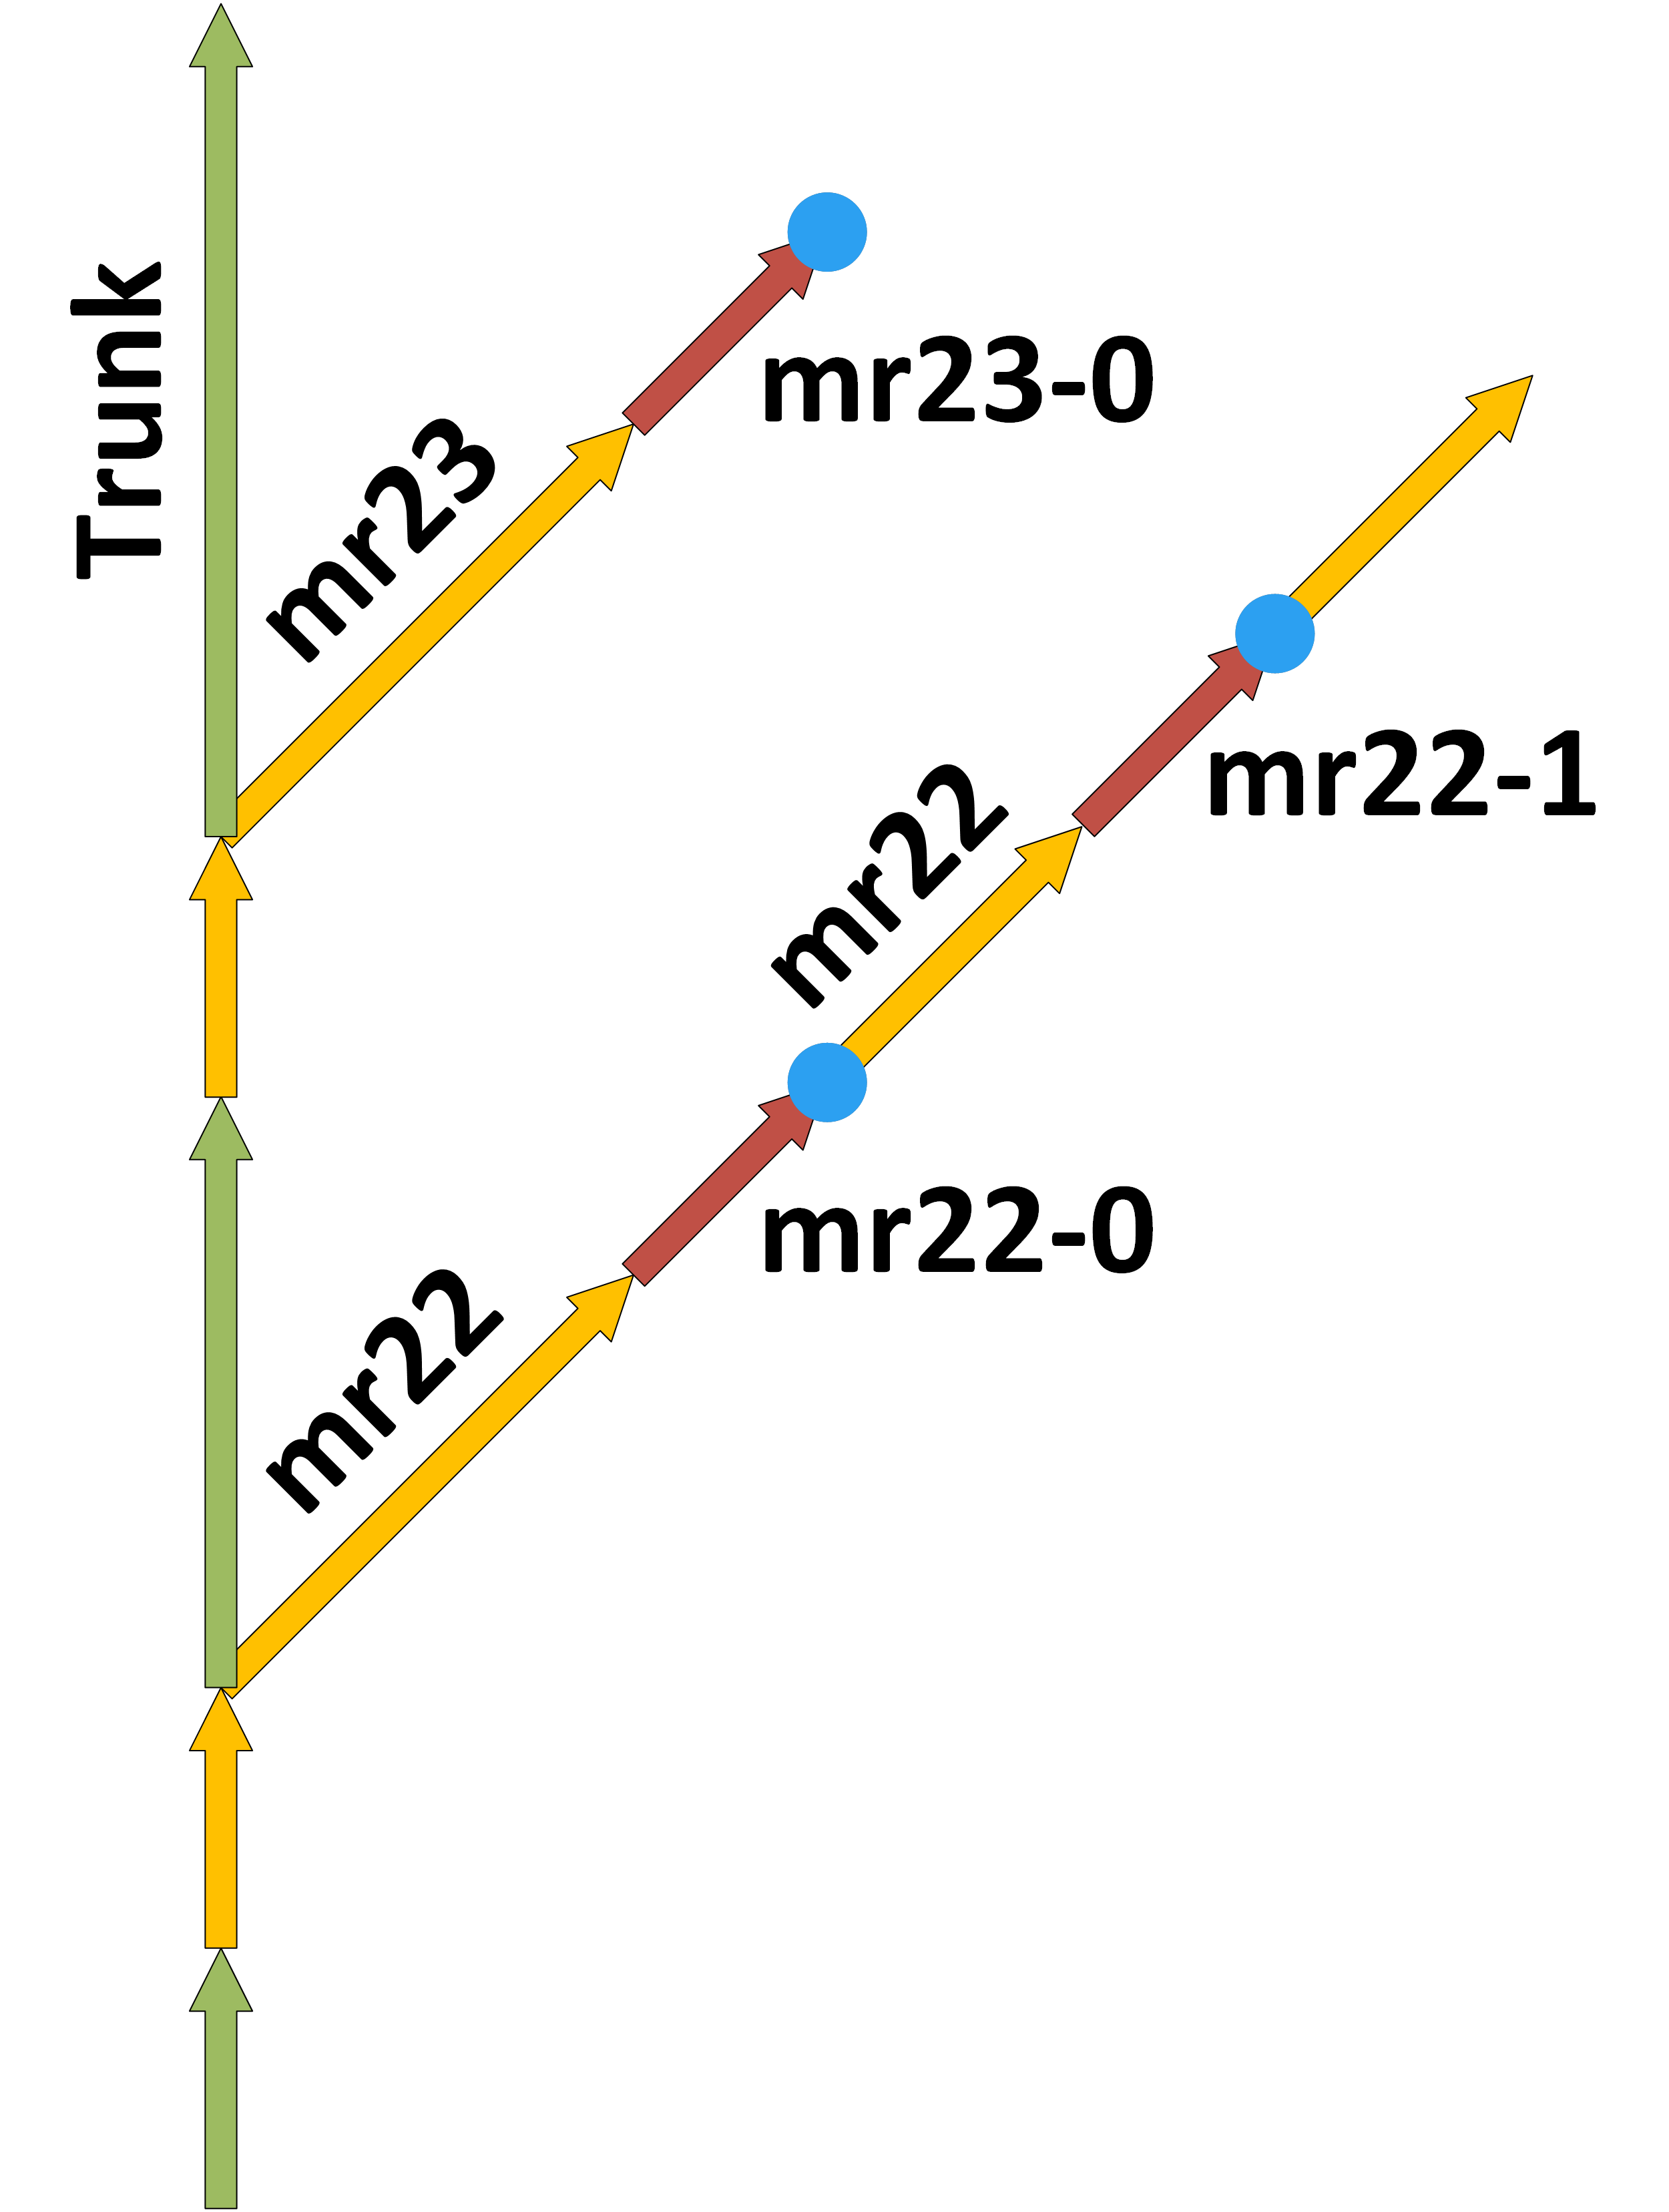
\includegraphics[height=5.5cm]{05_zones_old.png}
\end{figure}



\begin{figure}
  \centering
  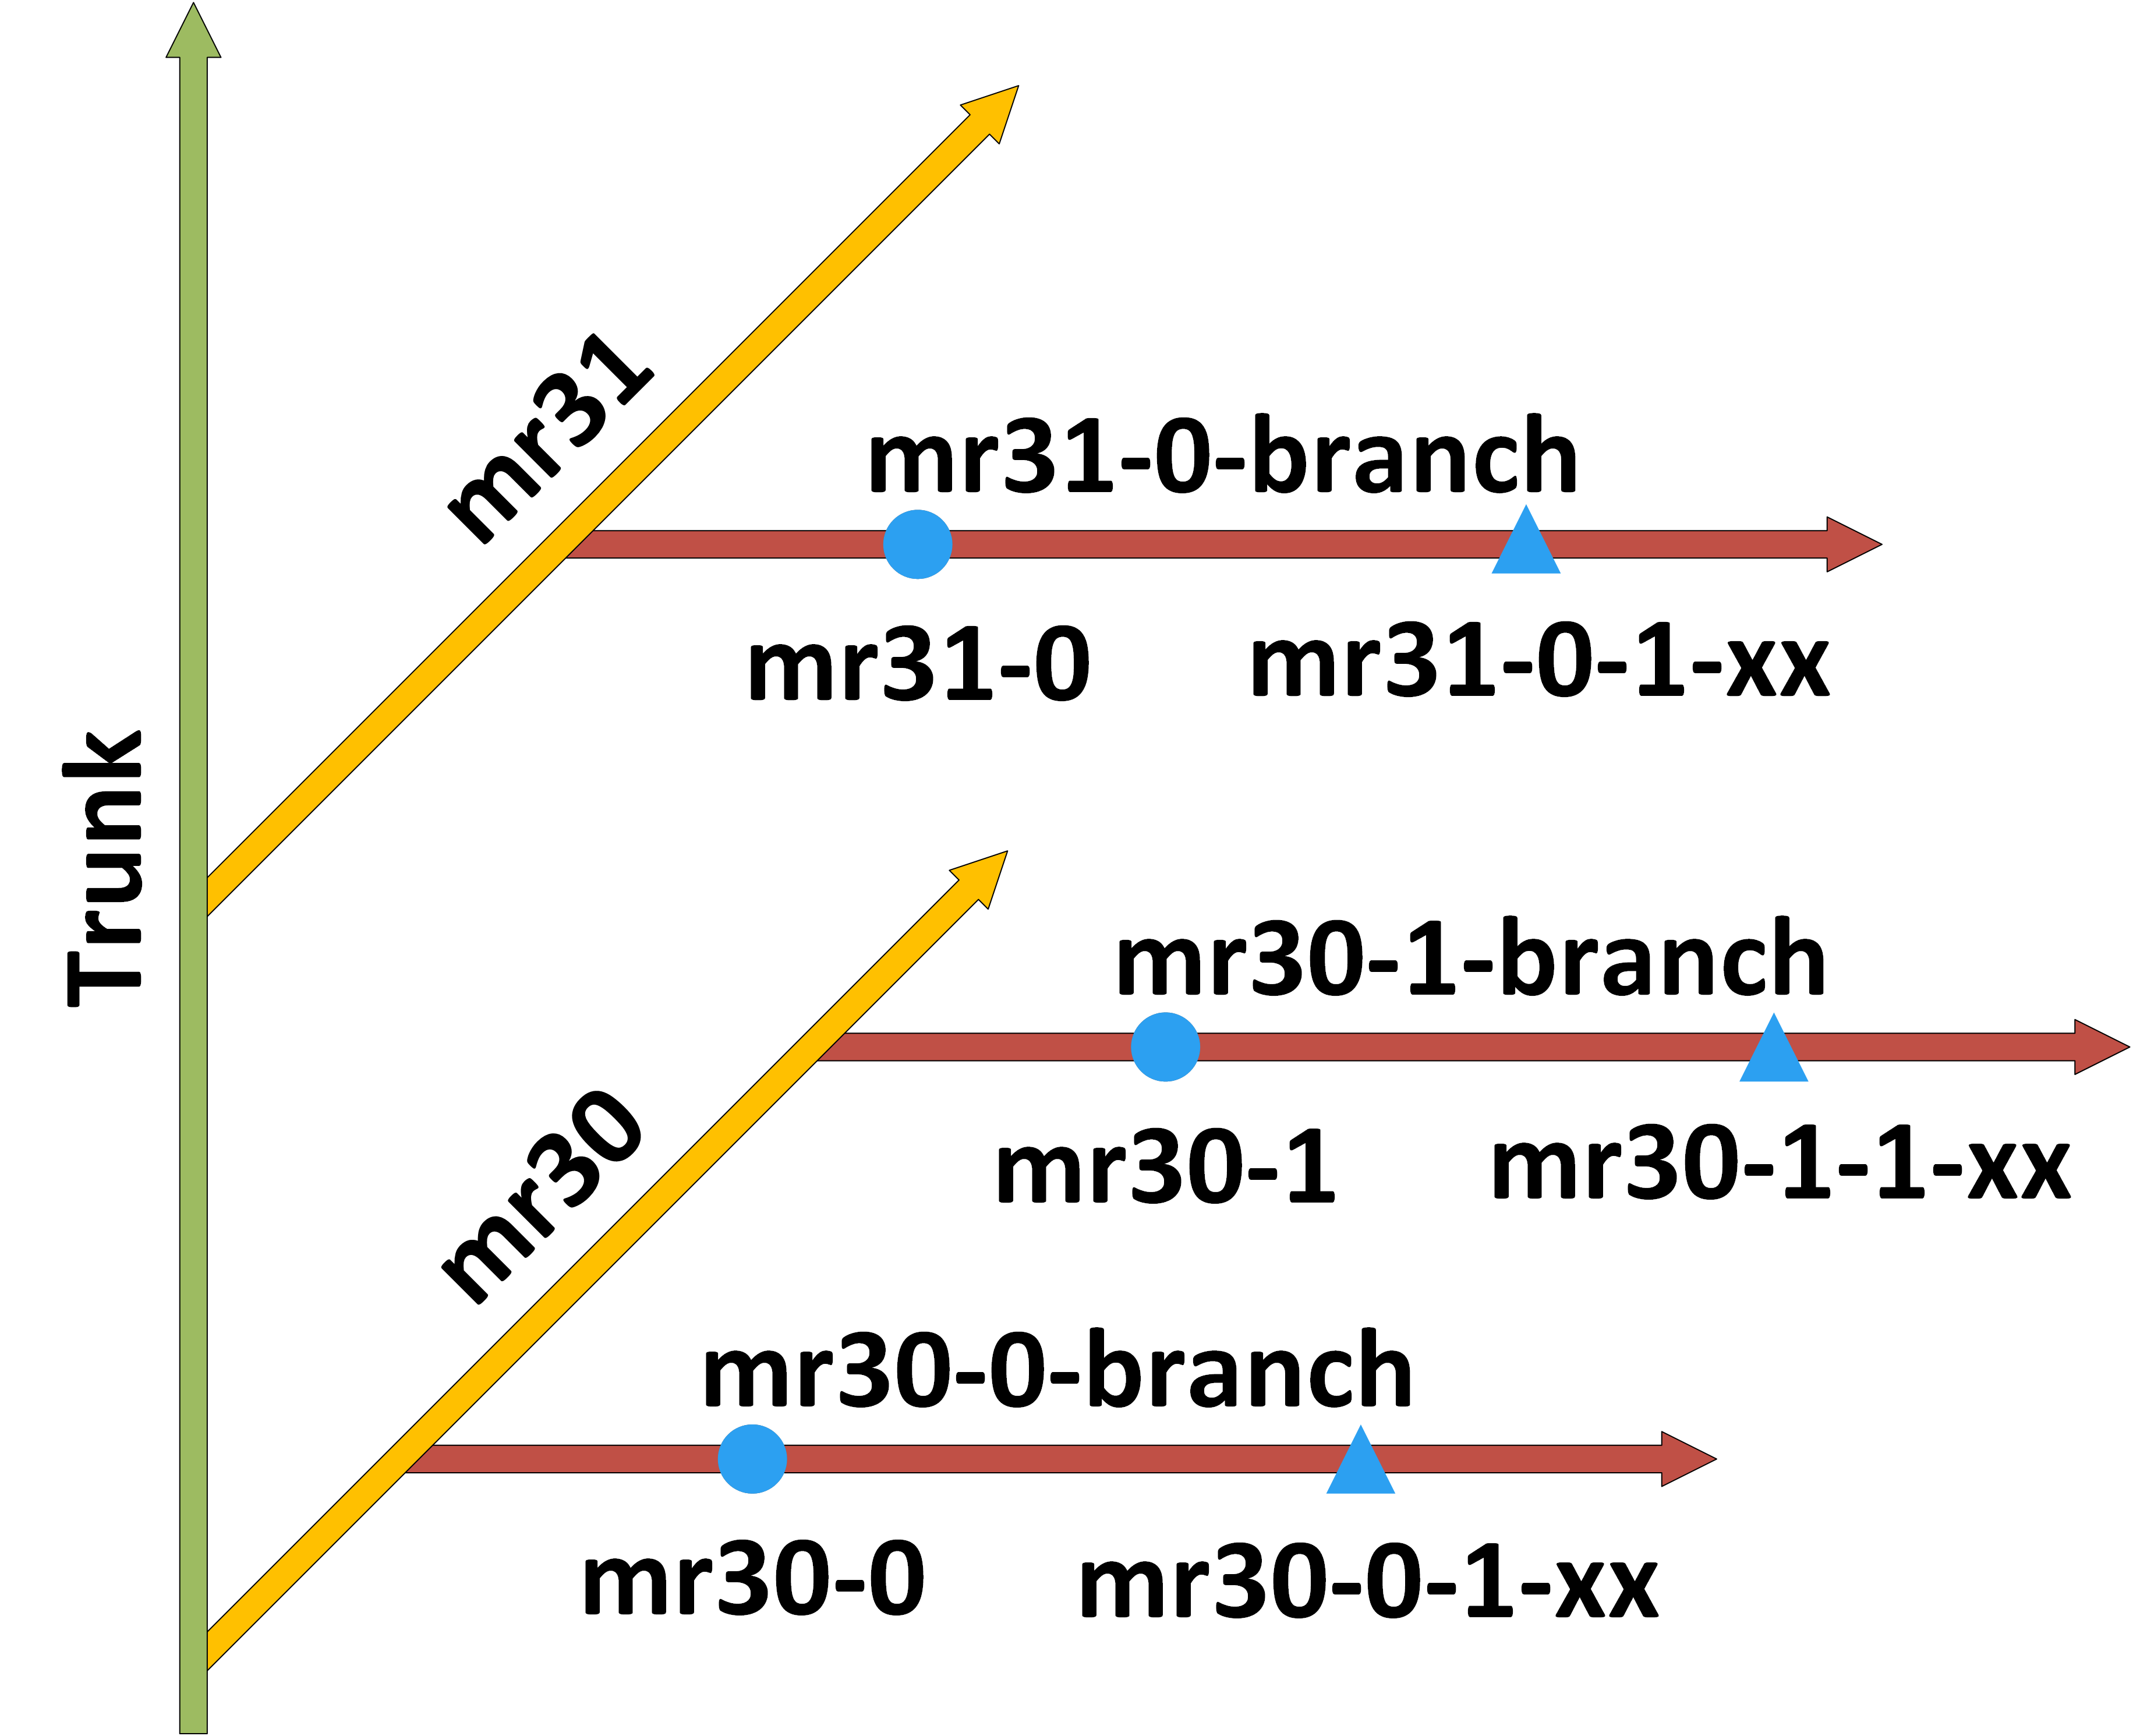
\includegraphics[width=6cm]{05_zones.png}
\end{figure}

Главная ветвь разработки (trunk/master) всегда открыта для приема любых новых функциональных возможностей.

В определенный момент времени (по календарю) от главной ветви <<отщепляется>> новая ветвь, в которой будет проходить стабилизация готовых на тот момент программных возможностей. Эта ветвь сразу становится желтой, т.~е. в неё запрещено добавлять новые возможности, только стабилизировать текущие.

В определенный момент времени от желтой ветви отщепляется красная ветвь. В красную ветвь можно коммитить только по запросу QA отдела.
В определенный момент времени (по календарю), на красной ветви проставляется аннотированная метка (тег) нового релиза.
К этому моменту отдел QA должен завершить тестирование новой версии продукта. Если какие"=то новые программные возможности не готовы и блокируют выпуск новой версии, они должны быть удалены.

Если после проставления аннотированной метки, заказчик или отдел поддержки/эксплуатации находит критический баг, тогда отдел QA запрашивает коммит с исправлением в красную ветвь. После этого на красной ветви проставляется аннотированная метка хотфикса.
Данный подход позволяет разработчикам фиксировать изменения в любой момент времени, потому что главная ветка проекта всегда готова к приему любых изменений, желтые ветки в любой момент готовы к приему исправлений.

\subsection*{Наращивание новых функций и стабильность}

Есть два типа заказчиков: первые хотят стабильности, вторые заказывают новые функциональные возможности и стремятся ими воспользоваться как можно раньше.

Для первого типа заказчиков предлагается раз в год выпускать Long Term Support (LTS) релиз (релиз "--- это нулевой билд, x.0 версия), который будет стабилизироваться в течении года выпуском 6 билдов (версии x.1, x.2 и т.д.) только с исправлениями.
Для второго типа заказчиков предлагается переходить на обычные релизы по мере их выхода. Зачастую в очень сложных проектах новые программные возможности не всегда удовлетворяют заказчика с первого раза. Потому, чаще всего, после сдачи новых возможностей, заказчику нужно немного исправить поведение продукта. Поэтому для каждого обычного релиза выпускается один стабилизационный билд.
Заказчику нужно некоторое время для запуска новой версии продукта в промышленное использование, потому после выхода нового релиза команда разработчиков сразу приступает к выпуску стабилизационного билда к предыдущему релизу. Одновременно с этим разработчики бекпортируют все правки в LTS релиз и выпускают стабилизационный билд для LTS тоже. Т.е. разработчики не ждут отзыва заказчиков, для которых был выпущен новый релиз, а исправляют предыдущий, на который к этому моменту собраны жалобы.

~

\begin{figure}
  \centering
  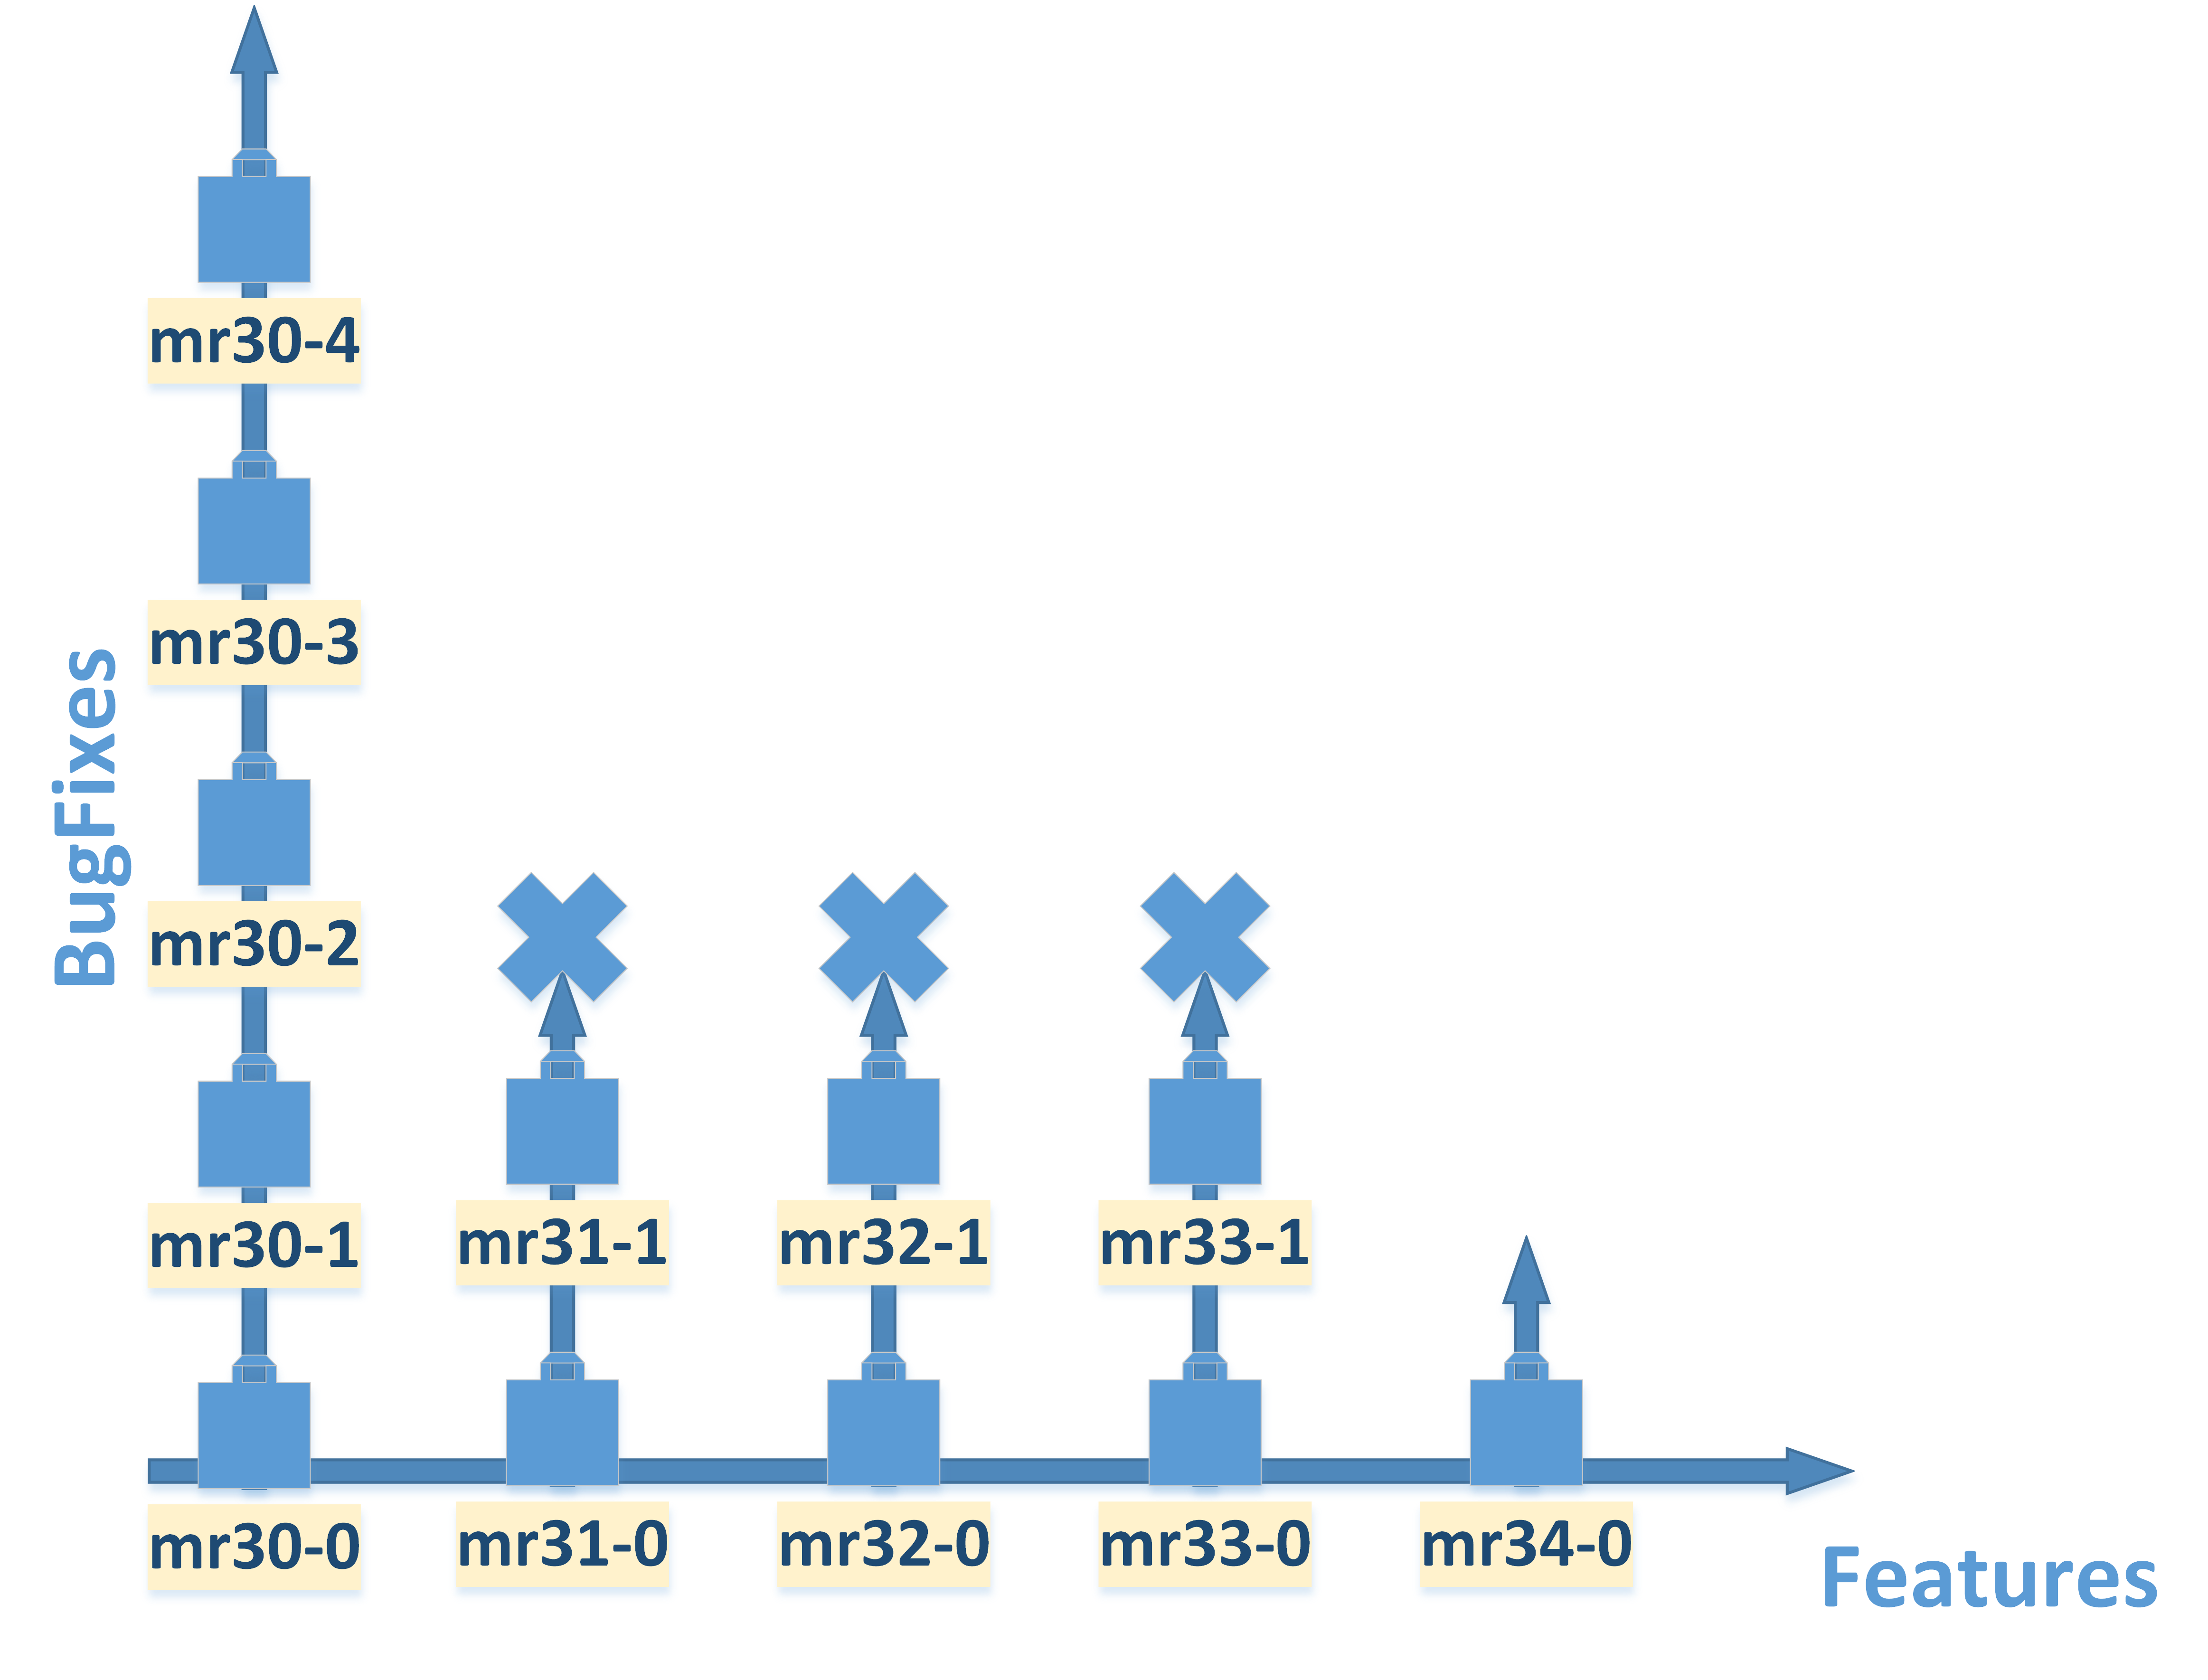
\includegraphics[width=10cm]{05_releases_graph_report.png}
\end{figure}

Данный поход позволяет:

\begin{enumerate}
  \item дать стабильность в LTS релизах;
  \item держать высокий темп выхода новых версий для заказчиков;
  \item продолжать заниматься разработкой, а не ожидать фидбека/багрепортов;
  \item стабилизировать новые версии по мере получения фидбека/багрепортов.
\end{enumerate}

\subsection*{Цикл разработки}

Заказчики хотят получать оплаченные новые возможности точно в срок.
На первый взгляд опыт разработки показывает, что это невозможно. Но это не так. Любые даже самые большие задачи могут быть разбиты на мелкие подзадачи, время на разработку которых возможно подсчитать. При относительно большом цикле (спринте), количество мелких задач, которые могут быть выполнены за определенный срок, стабильно. Не все задачи будут выполнены, но при правильном подсчете этот процент будет мал. В процессе фактической разработки может возникнуть определенное количество новых задач, они тоже должны быть заложены в план. Правильный подсчет времени и количества мелких задач, которые может выполнить отдел разработки в целом,  зависит от грамотности лидеров групп (team lead).

Был предложен следующий цикл разработки:

\begin{figure}[h!]
  \centering
  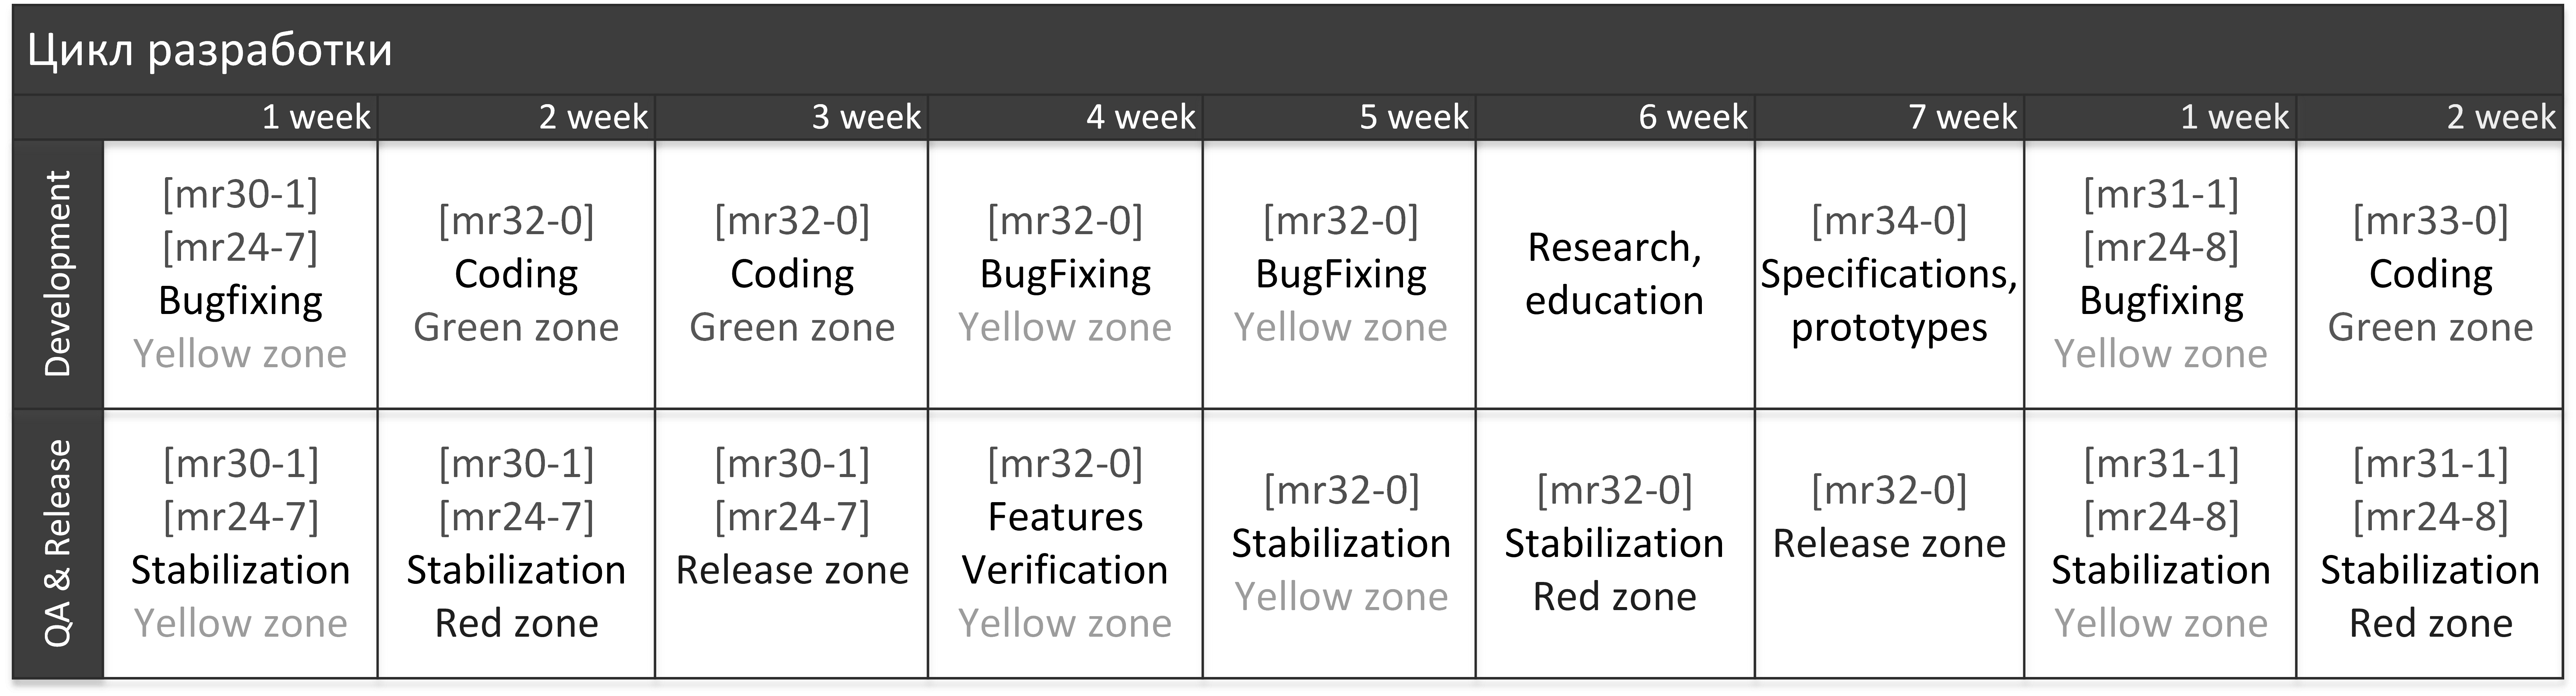
\includegraphics[width=11cm]{05_circle_v3.png}
\end{figure}

\subsection*{Создание спецификаций}

Невозможно гарантировать разработку новых возможностей вовремя, если конечному разработчику не понятны требования заказчика. Потому никакие запросы на новые возможности не будут приняты от заказчика (и не будут названы сроки) пока не будет создана исчерпывающая спецификация, которую примет и заказчик и лидеры групп в отделе разработки. Спецификация должна быть полностью понятна лидерам групп, которые разобьют ее на подзадачи и подсчитают сколько нужно времени на реализацию каждой из них, только после этого заказчику будут названы сроки.

\subsection*{Быстрое развертывание среды разработки}

Используемые OpenSource решения "--- Jenkins, VirtualBox, Vagrant.

Каждому разработчику, что бы начать исправлять ошибку или писать код, нужно иметь личную систему с установленной копией продукта который он разрабатывает. В больших и сложных продуктах довольно долго подготавливать правильно установленный и настроенный продукт (например, базу данных Oracle), это может длиться от нескольких часов до нескольких суток. При высоком темпе выпуска новых версий эта проблема многократно усиливается. Чтобы ускорить процесс развертывания среды разработки был полностью автоматизирован процесс создания образов виртуальных машин для всех версий продукта, для всех платформ с помощью Jenkins CI. Эти образы используются в самом Jenkins для запуска тестов во всех поддерживаемых версиях продукта на всех возможных платформах. С помощью vagrant, гигабитной офисной сети и SSD разработчики могут разворачивать за считанные десятки секунд полностью готовую среду разработки из образа, который имеет актуальный код на нужной платформе.

\subsection*{Автоматизация тестирования}

Используемые OpenSource решения "--- Jenkins.
Код покрыт следующими видами тестов:

\begin{itemize}
  \item Unit test
  \item Functionality test
  \item Performance test
  \item Syntax test
  \item Style test
  \item Code analysis
  \item Compile test
  \item Memory leak test (valgrind)
\end{itemize}

\subsection*{Стабильный транк}

Используемые OpenSource решения "--- Git, Gerrit, gerrit"=tools, Jenkins CI.

~

~

\begin{figure}[b]
  \centering
  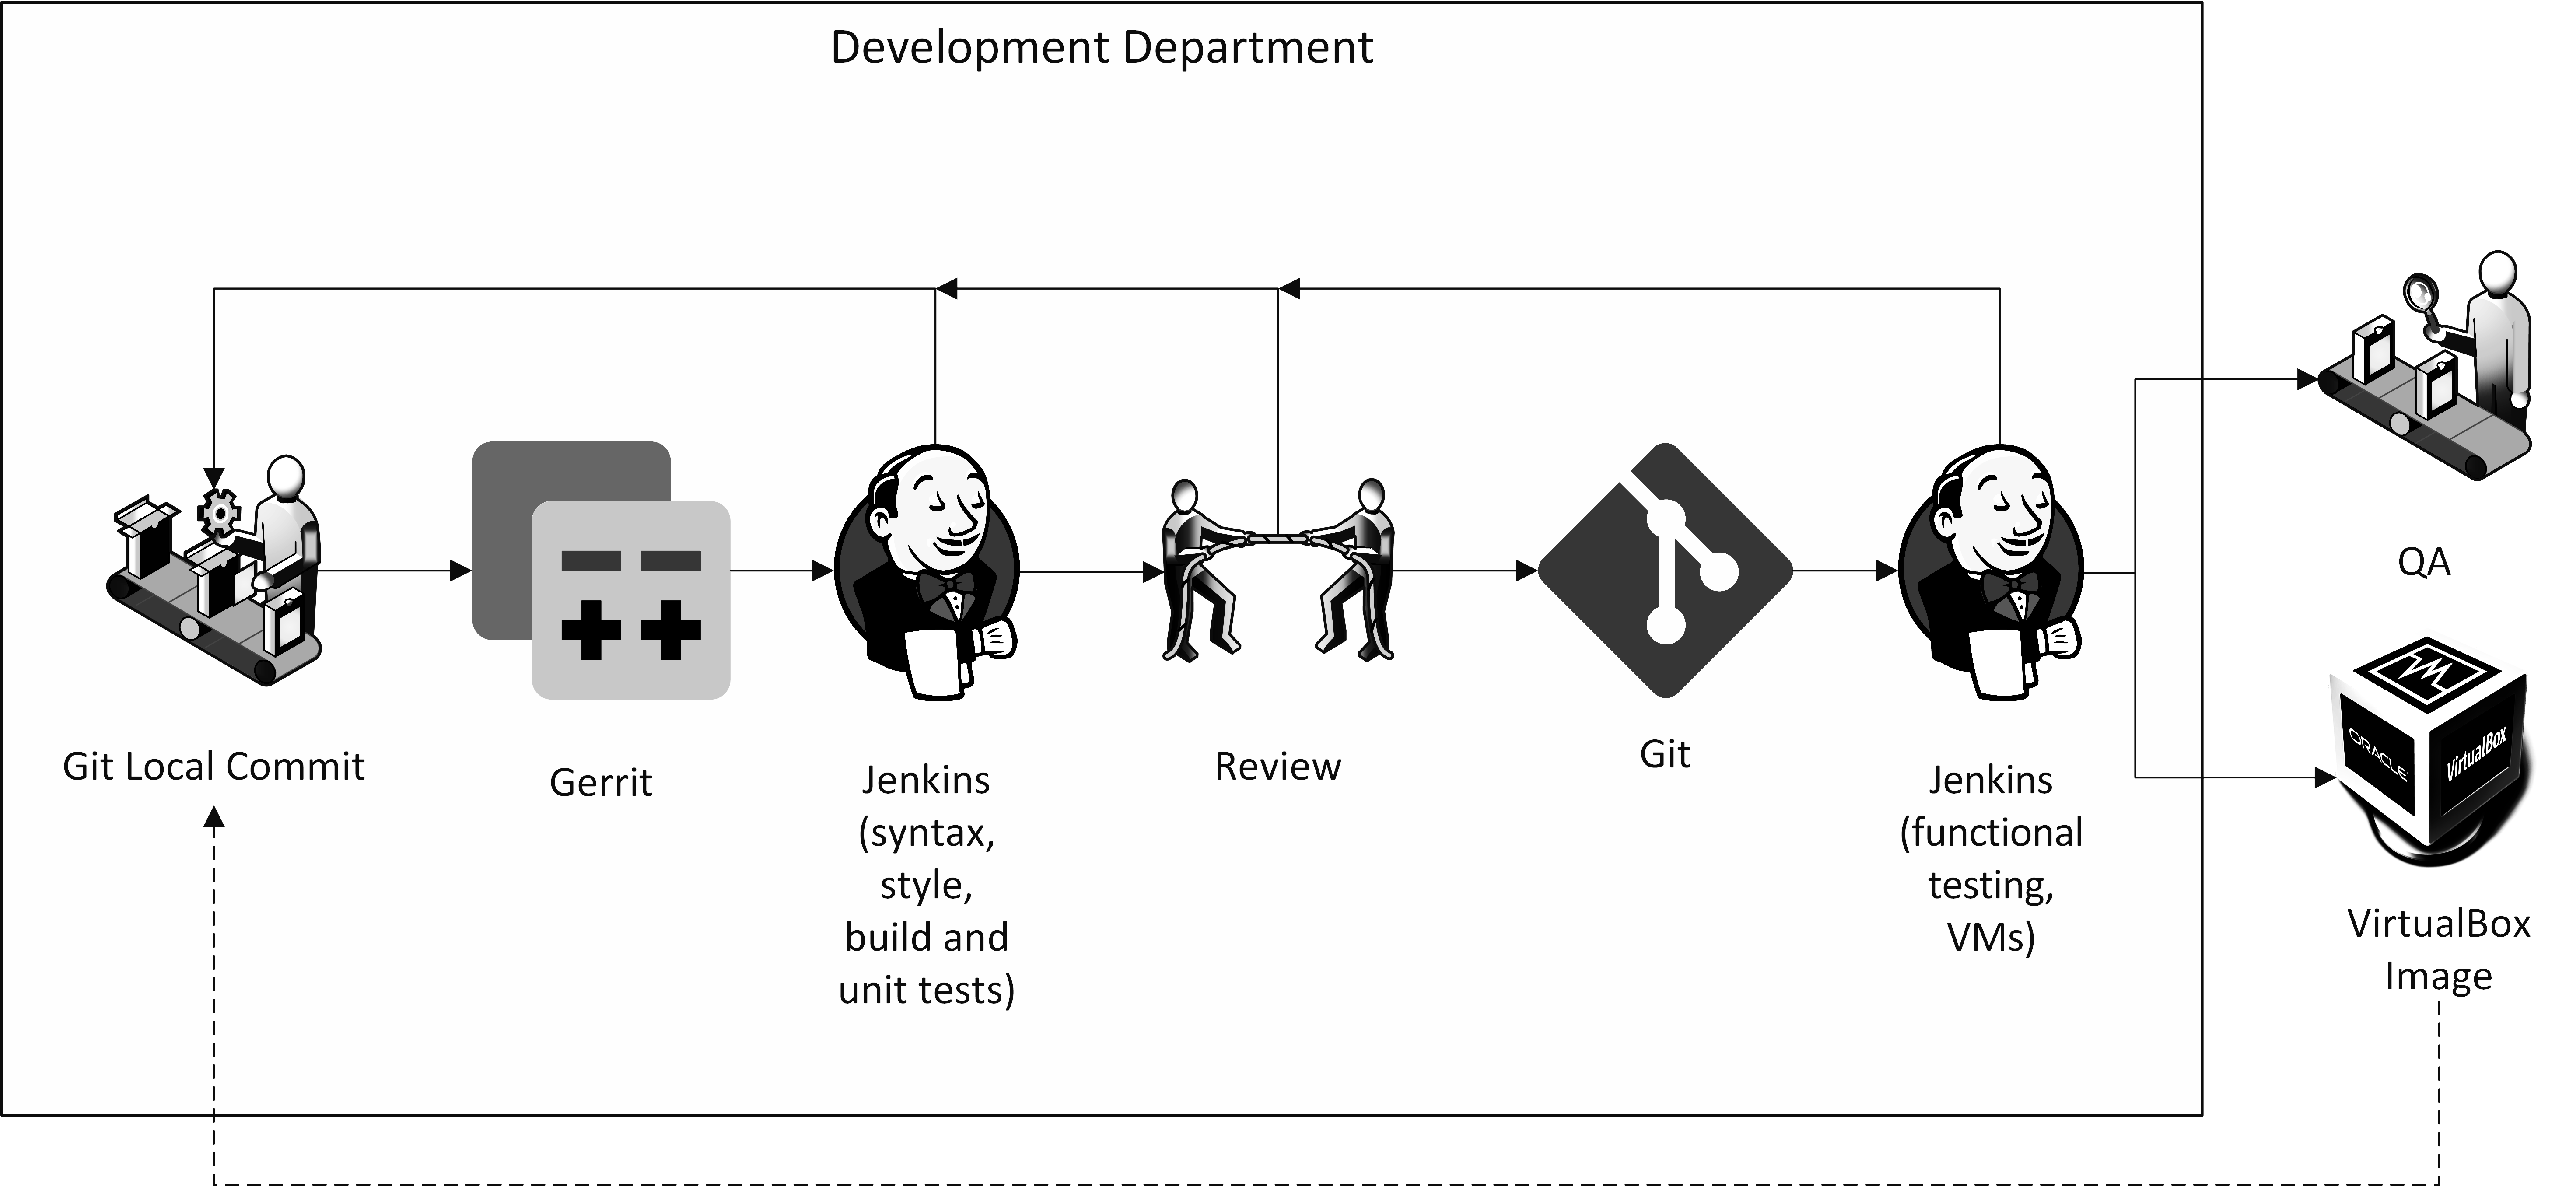
\includegraphics[width=11cm]{05_review.png} 
\end{figure}

Чтобы улучшить стабильность кода, был предложен следующий подход:

\begin{itemize}
  \item разработчик делает фиксацию изменений (коммит) в локальном git репозитории и запускает команду <<git review>>, которая отправляет изменения в gerrit.
  \item Gerrit задерживает изменения, не давая их отправить в центральный репозиторий до тех пор пока изменения не будут проверены рецензентами и автоматическими тестами в Jenkins.
  \item Gerrit тригерит запуск тестов в Jenkins, результат которых выставляется в виде положительной или негативной оценки.
  \item рецензенты могут комментировать код и выставлять оценки от -2 до +2. Код, который не имеет оценки +2 или имеет оценку -2 "--- не может попасть в центральный репозиторий.
  \item когда рецензенты и Jenkins проставили положительные оценки, появляется кнопка <<Submit>> с помощью которой можно пропустить изменения в центральный репозиторий.
  \item раз в день запускаются тяжелые функциональные тесты, которые могут длиться всю ночь.
  \item на основе кода формируются образы виртуальных машин, которые с утра будут загружены разработчиками и QA.
\end{itemize}

\subsection*{Выводы}

Предложенные организационные изменения были проведены в компании PortaOne, Inc. на команде разработчиков из 50 человек и позволили разработчикам больше заниматься любимым делом и выдавать на 30\% больше кода. Отношения с клиентами улучшились благодаря выходу точно в срок новых версий продукта с заказанными функциональными возможностями. Стабильность кода увеличилась за счет введения процедуры review и автоматизации тестирования.


\end{document}





\documentclass[10pt, a5paper]{article}
\usepackage{pdfpages}
\usepackage{parallel}
\usepackage[T2A]{fontenc}
\usepackage{ucs}
\usepackage[utf8x]{inputenc}
\usepackage[polish,english,russian]{babel}
\usepackage{hyperref}
\usepackage{rotating}
\usepackage[inner=2cm,top=1.8cm,outer=2cm,bottom=2.3cm,nohead]{geometry}
\usepackage{listings}
\usepackage{graphicx}
\usepackage{wrapfig}
\usepackage{longtable}
\usepackage{indentfirst}
\usepackage{array}
\newcolumntype{P}[1]{>{\raggedright\arraybackslash}p{#1}}
\frenchspacing
\usepackage{fixltx2e} %text sub- and superscripts
\usepackage{icomma} % коскі ў матэматычным рэжыме
\PreloadUnicodePage{4}

\newcommand{\longpage}{\enlargethispage{\baselineskip}}
\newcommand{\shortpage}{\enlargethispage{-\baselineskip}}

\def\switchlang#1{\expandafter\csname switchlang#1\endcsname}
\def\switchlangbe{
\let\saverefname=\refname%
\def\refname{Літаратура}%
\def\figurename{Іл.}%
}
\def\switchlangen{
\let\saverefname=\refname%
\def\refname{References}%
\def\figurename{Fig.}%
}
\def\switchlangru{
\let\saverefname=\refname%
\let\savefigurename=\figurename%
\def\refname{Литература}%
\def\figurename{Рис.}%
}

\hyphenation{admi-ni-stra-tive}
\hyphenation{ex-pe-ri-ence}
\hyphenation{fle-xi-bi-li-ty}
\hyphenation{Py-thon}
\hyphenation{ma-the-ma-ti-cal}
\hyphenation{re-ported}
\hyphenation{imp-le-menta-tions}
\hyphenation{pro-vides}
\hyphenation{en-gi-neering}
\hyphenation{com-pa-ti-bi-li-ty}
\hyphenation{im-pos-sible}
\hyphenation{desk-top}
\hyphenation{elec-tro-nic}
\hyphenation{com-pa-ny}
\hyphenation{de-ve-lop-ment}
\hyphenation{de-ve-loping}
\hyphenation{de-ve-lop}
\hyphenation{da-ta-ba-se}
\hyphenation{plat-forms}
\hyphenation{or-ga-ni-za-tion}
\hyphenation{pro-gramming}
\hyphenation{in-stru-ments}
\hyphenation{Li-nux}
\hyphenation{sour-ce}
\hyphenation{en-vi-ron-ment}
\hyphenation{Te-le-pathy}
\hyphenation{Li-nux-ov-ka}
\hyphenation{Open-BSD}
\hyphenation{Free-BSD}
\hyphenation{men-ti-on-ed}
\hyphenation{app-li-ca-tion}

\def\progref!#1!{\texttt{#1}}
\renewcommand{\arraystretch}{2} %Іначай формулы ў матрыцы зліпаюцца з лініямі
\usepackage{array}

\def\interview #1 (#2), #3, #4, #5\par{

\section[#1, #3, #4]{#1 -- #3, #4}
\def\qname{LVEE}
\def\aname{#1}
\def\q ##1\par{{\noindent \bf \qname: ##1 }\par}
\def\a{{\noindent \bf \aname: } \def\qname{L}\def\aname{#2}}
}

\def\interview* #1 (#2), #3, #4, #5\par{

\section*{#1\\{\small\rm #3, #4. #5}}

\def\qname{LVEE}
\def\aname{#1}
\def\q ##1\par{{\noindent \bf \qname: ##1 }\par}
\def\a{{\noindent \bf \aname: } \def\qname{L}\def\aname{#2}}
}


\begin{document}

\title{Сеть хранения данных своими руками}%\footnote{Текст данных и последующих тезисов, кроме специально оговоренных случаев, доступен под лицензией Creative Commons Attribution-ShareAlike 3.0}

\author{Роман Шишнев\footnote{Минск, Беларусь; \url{rommer@active.by}}}
\maketitle

\begin{abstract}
There is a small gap in ready solutions between the systems with a local disks and a professional storage systems. The report highlights some technologies and approaches helpful at building personal storage area network of arbitrary size for using in various environments.
\end{abstract}

В настоящее время есть небольшой разрыв между готовыми системами, использующими локальные диски для хранения данных, и профессиональными системами хранения данных. Рассмотрим некоторые современные технологии, которые могут помочь самостоятельно построить сеть хранения данных (СХД) практически любого масштаба для применения в самых различных средах.

На первом шаге постороения личной СХД необходимо определить параметры её производительности и доступность. Ключеными моментами для СХД являются:

\begin{itemize}
  \item объем дискового простанства;
  \item производительность в IOPS (операций ввода-вывода в секунду);
  \item latency (среднее время доступа к данным);
  \item пропускная способность сети;
  \item допустимое время простоя.
\end{itemize}

На обьеме доступного простанства останавливаться не будем, так как тот параметр зависит исключительно от задачи.

Произодительность в количестве операций ввода/вывода в секунду следует рассматривать как ключевой параметр системы. Для примера, один диск SATA с 7200 оборотами в секунду позволяет выполнять около 100 операций при случайном доступе. Именно требуемое количество IOPS для СХД в основном и определяет тип и колическов дисков в нашей системе.

Latency в большей степени также зависит от дисков. Но при достаточно быстрых дисках, например SSD, стоит уже учитывать и задержки, которые возникают в сети при передаче данных.

Пропускная способность сети определяет максимальную скорость, на которой можно будет выполнять операции чтения и записи на системе хранения данных. В зависимости от задачи сеть можно создавать медленном медном гигабитном Ethernet, на 10-ти гигабитной оптике, либо на высокосторостном fiber channel.

Допустимое время простоя определяет количесво дублированных компонентов в сети и системе хранения данных.

Теперь рассмотрим самую простую задачу:

\begin{itemize}
  \item сервер \verb!A!, в котором установлен один SATA"=диск;
  \item сервер \verb!B!, которому нужно получить доступ к этому диску;
  \item гигабитные сетевые карты на каждом из серверов.
\end{itemize}

Для получения доступа к этому диску по сети Ethernet нужно выбрать протокол передачи данных. Самым простым и удобным протоколом в данном случае является iSCSI -- это по сути SCSI"=протокол поверх TCP/IP. На сервер \verb!A! нужно будет установить ПО, которое реализует так называемый iSCSI"=таргет "--- именно он будет осуществлять доступ к диску. На сервере \verb!B! должен быть установлен iSCSI"=инициатор "--- он будет подключаться к дискам. После установки и настройки сервер \verb!B! будет видеть диск сервера \verb!A! так, как будто он локальный.

Добавим в схему сервер \verb!C!, которому также нужен доступ к этому диску.

Для этого схему нужно просто дополнить гигабитным коммутатором, к которому теперь будут подключены все 3 сервера. На сервере \verb!C! достаточно установить / настроить iSCSI"=инициатор и подключить к iSCSI"=таргету на сервере \verb!A!.

После приведенных манипуляций серверы \verb!B! и \verb!C! <<видят>> один и тот же диск.

Имеет смысл предусмотреть также меры по устанению единых точек отказа в системе, и опционально "--- варианты маштабирования системы до десятков и сотен дисков и серверов.

\end{document}





\documentclass[10pt, a5paper]{article}
\usepackage{pdfpages}
\usepackage{parallel}
\usepackage[T2A]{fontenc}
\usepackage{ucs}
\usepackage[utf8x]{inputenc}
\usepackage[polish,english,russian]{babel}
\usepackage{hyperref}
\usepackage{rotating}
\usepackage[inner=2cm,top=1.8cm,outer=2cm,bottom=2.3cm,nohead]{geometry}
\usepackage{listings}
\usepackage{graphicx}
\usepackage{wrapfig}
\usepackage{longtable}
\usepackage{indentfirst}
\usepackage{array}
\newcolumntype{P}[1]{>{\raggedright\arraybackslash}p{#1}}
\frenchspacing
\usepackage{fixltx2e} %text sub- and superscripts
\usepackage{icomma} % коскі ў матэматычным рэжыме
\PreloadUnicodePage{4}

\newcommand{\longpage}{\enlargethispage{\baselineskip}}
\newcommand{\shortpage}{\enlargethispage{-\baselineskip}}

\def\switchlang#1{\expandafter\csname switchlang#1\endcsname}
\def\switchlangbe{
\let\saverefname=\refname%
\def\refname{Літаратура}%
\def\figurename{Іл.}%
}
\def\switchlangen{
\let\saverefname=\refname%
\def\refname{References}%
\def\figurename{Fig.}%
}
\def\switchlangru{
\let\saverefname=\refname%
\let\savefigurename=\figurename%
\def\refname{Литература}%
\def\figurename{Рис.}%
}

\hyphenation{admi-ni-stra-tive}
\hyphenation{ex-pe-ri-ence}
\hyphenation{fle-xi-bi-li-ty}
\hyphenation{Py-thon}
\hyphenation{ma-the-ma-ti-cal}
\hyphenation{re-ported}
\hyphenation{imp-le-menta-tions}
\hyphenation{pro-vides}
\hyphenation{en-gi-neering}
\hyphenation{com-pa-ti-bi-li-ty}
\hyphenation{im-pos-sible}
\hyphenation{desk-top}
\hyphenation{elec-tro-nic}
\hyphenation{com-pa-ny}
\hyphenation{de-ve-lop-ment}
\hyphenation{de-ve-loping}
\hyphenation{de-ve-lop}
\hyphenation{da-ta-ba-se}
\hyphenation{plat-forms}
\hyphenation{or-ga-ni-za-tion}
\hyphenation{pro-gramming}
\hyphenation{in-stru-ments}
\hyphenation{Li-nux}
\hyphenation{sour-ce}
\hyphenation{en-vi-ron-ment}
\hyphenation{Te-le-pathy}
\hyphenation{Li-nux-ov-ka}
\hyphenation{Open-BSD}
\hyphenation{Free-BSD}
\hyphenation{men-ti-on-ed}
\hyphenation{app-li-ca-tion}

\def\progref!#1!{\texttt{#1}}
\renewcommand{\arraystretch}{2} %Іначай формулы ў матрыцы зліпаюцца з лініямі
\usepackage{array}

\def\interview #1 (#2), #3, #4, #5\par{

\section[#1, #3, #4]{#1 -- #3, #4}
\def\qname{LVEE}
\def\aname{#1}
\def\q ##1\par{{\noindent \bf \qname: ##1 }\par}
\def\a{{\noindent \bf \aname: } \def\qname{L}\def\aname{#2}}
}

\def\interview* #1 (#2), #3, #4, #5\par{

\section*{#1\\{\small\rm #3, #4. #5}}

\def\qname{LVEE}
\def\aname{#1}
\def\q ##1\par{{\noindent \bf \qname: ##1 }\par}
\def\a{{\noindent \bf \aname: } \def\qname{L}\def\aname{#2}}
}


\begin{document}

\title{Использование Ejudge для проведения олимпиад по программированию}%\footnote{Текст данных и последующих тезисов, кроме специально оговоренных случаев, доступен под лицензией Creative Commons Attribution-ShareAlike 3.0}

\author{Дмитрий Храбров\footnote{Гомель, Беларусь; ГГТУ им. П.О. Сухого; \url{root@dexp.in}}}
\maketitle

\begin{abstract}
The paper considers usage of open source online programming competitions server ejudge. In addition to technical aspects \linebreak author's personal experience is described, concerning both \linebreak technical and social issues.
\end{abstract}

 Как сказано на официальном сайте, Ejudge "--- это система для проведения различных мероприятий, в которых необходима автоматическая проверка программ. Система может применяться для проведения олимпиад и поддержки учебных курсов. Ejudge распространяется под лицензией GPL, имеет многоязычный веб"=интерфейс и поддерживает защищённое исполнение программ (если установлен патч к ядру Linux). Также система активно используется для проведения олимпиад в различных учебных заведениях, и, по опыту, олимпиады на этой системе проходили успешно.

Для проведения олимпиады необходимо зарегистрировать участников: лично или командно. Далее нужно дать участникам возможность читать условия задач и отправлять решения на тестирование. Перед отсылкой на тестирование участник выбирает компилятор и файл с исходным кодом решения. Далее система на сервере пытается скомпилировать решение с помощью выбранного компилятора. Если произошли ошибки, то участнику выдаётся сообщение. Если компиляция прошла успешно, то происходит непосредственно тестирование. Исполняемому файлу на вход (STDIN или файл) подаются входные данные, заранее сформированные автором задачи. На выполнение обычно ставятся ограничения по времени и по памяти. Если решение участника уложилось в лимиты и выдало ответ, система сверяет этот ответ с авторским. Кроме того система должна вести статистику, показывать положение участников. 

Установка и настройка Ejudge подробно описана на сайте проекта, также есть пошаговые инструкции. Через пакетный менеджер дистрибутива нужно установить необходимые компиляторы, Ejudge при конфигурировании автоматически их подхватит. Так же перед установкой нужно указать пути директорий турниров, веб"=сервера и так далее. После установки надо не забыть запустить демон Ejudge, иначе будет показываться сообщение об ошибке. На случай, если нет желания или возможности выполнять установку и настройку, на официальном сайте лежит готовый и настроенный VirtualBox"=образ.

На официальном сайте Ejudge написано, что она имеет настраиваемый внешний вид. При беглом просмотре такая возможность без перекомпиляции найдена не была. Все страницы свёрстаны абсолютным позиционированием элементов, через CSS трудно поддаются изменениям. Так что мы при использовании системы ограничились заменой логотипа и фона страницы, после чего Ejudge не перестала быть собой в плане не слишком удобного интерфейса, однако стала гораздо более привлекательной.

На текущий момент нами успешно проведена на Ejudge внутривузовская олимпиада по программированию. Наиболее востребованы языки: C\#, Java, C, Pascal. Mono "--- реализация C\# в Linux. Были опасения, что реализация будет отличаться, и студенты будут жаловаться, что C\# не работает. Однако Mono отработало без нареканий. Java поддерживается нативно, однако для этого требуется минимум 512 мегабайт памяти, что необходимо учитывать "--- например, при конфигурировании виртуальной машины. Компиляторов С/С++ нами предоставлялось студентам два: gcc и clang. Студенты периодически путали их и отправляли Си"=программу на тестирование компилятором g++ (для языка С++), однако негативных последствий это не имело. Наибольшее недопонимание вызывало отсутствие заголовочных файлов windows.h и conio.h, которые студенты не задумываясь вставляли в свои программы. Приходилось ходить по аудиториям и повторять, что эти файлы подключать нельзя. Из компиляторов Pascal ограничились Free Pascal, так как этот язык в ВУЗе используется всё меньше; фактически, он был оставлен только для совместимости.

Двое человек спросили о поддержке PHP и Brainfuck. Интерпретатор РНР на сервере установлен и доступен для тестирования приложений. Студенту был предоставлен пример программы, но писать на РНР он не рискнул, так как в аудиториях РНР не установлен. Язык Brainfuck системой Ejudge по умолчанию не поддерживается; студенту пообещали, что язык будет добавлен, если студент гарантирует, что будет на нём писать олимпиаду, после чего вопрос иссяк.

Из неожиданных моментов следует отметить то, что Ejudge по умолчанию считает C\# <<небезопасным>> языком, и он отключен для использования в турнирах. Ещё один тонкий момент был обнаружен после проведения олимпиады "--- система отказалась показать таблицу результатов студентам (пришлось воспользоваться для показа администраторским интерфейсом). Как выяснилось, Ejudge по умолчанию показывает таблицу через 2 часа после завершения олимпиады, однако это настраивается в веб"=интерфейсе.

В целом система тестирования Ejudge показала себя очень неплохо: свою задачу выполняет, поддерживает все современные языки программирования, имеет большое количество настраиваемых возможностей, почти всё доступно через веб"=интерфейс. Из отрицательных черт можно отметить не совсем логичный и удобный интерфейс, причём как турнирный, так и администраторский.


\end{document}





\documentclass[10pt, a5paper]{article}
\usepackage{pdfpages}
\usepackage{parallel}
\usepackage[T2A]{fontenc}
\usepackage{ucs}
\usepackage[utf8x]{inputenc}
\usepackage[polish,english,russian]{babel}
\usepackage{hyperref}
\usepackage{rotating}
\usepackage[inner=2cm,top=1.8cm,outer=2cm,bottom=2.3cm,nohead]{geometry}
\usepackage{listings}
\usepackage{graphicx}
\usepackage{wrapfig}
\usepackage{longtable}
\usepackage{indentfirst}
\usepackage{array}
\newcolumntype{P}[1]{>{\raggedright\arraybackslash}p{#1}}
\frenchspacing
\usepackage{fixltx2e} %text sub- and superscripts
\usepackage{icomma} % коскі ў матэматычным рэжыме
\PreloadUnicodePage{4}

\newcommand{\longpage}{\enlargethispage{\baselineskip}}
\newcommand{\shortpage}{\enlargethispage{-\baselineskip}}

\def\switchlang#1{\expandafter\csname switchlang#1\endcsname}
\def\switchlangbe{
\let\saverefname=\refname%
\def\refname{Літаратура}%
\def\figurename{Іл.}%
}
\def\switchlangen{
\let\saverefname=\refname%
\def\refname{References}%
\def\figurename{Fig.}%
}
\def\switchlangru{
\let\saverefname=\refname%
\let\savefigurename=\figurename%
\def\refname{Литература}%
\def\figurename{Рис.}%
}

\hyphenation{admi-ni-stra-tive}
\hyphenation{ex-pe-ri-ence}
\hyphenation{fle-xi-bi-li-ty}
\hyphenation{Py-thon}
\hyphenation{ma-the-ma-ti-cal}
\hyphenation{re-ported}
\hyphenation{imp-le-menta-tions}
\hyphenation{pro-vides}
\hyphenation{en-gi-neering}
\hyphenation{com-pa-ti-bi-li-ty}
\hyphenation{im-pos-sible}
\hyphenation{desk-top}
\hyphenation{elec-tro-nic}
\hyphenation{com-pa-ny}
\hyphenation{de-ve-lop-ment}
\hyphenation{de-ve-loping}
\hyphenation{de-ve-lop}
\hyphenation{da-ta-ba-se}
\hyphenation{plat-forms}
\hyphenation{or-ga-ni-za-tion}
\hyphenation{pro-gramming}
\hyphenation{in-stru-ments}
\hyphenation{Li-nux}
\hyphenation{sour-ce}
\hyphenation{en-vi-ron-ment}
\hyphenation{Te-le-pathy}
\hyphenation{Li-nux-ov-ka}
\hyphenation{Open-BSD}
\hyphenation{Free-BSD}
\hyphenation{men-ti-on-ed}
\hyphenation{app-li-ca-tion}

\def\progref!#1!{\texttt{#1}}
\renewcommand{\arraystretch}{2} %Іначай формулы ў матрыцы зліпаюцца з лініямі
\usepackage{array}

\def\interview #1 (#2), #3, #4, #5\par{

\section[#1, #3, #4]{#1 -- #3, #4}
\def\qname{LVEE}
\def\aname{#1}
\def\q ##1\par{{\noindent \bf \qname: ##1 }\par}
\def\a{{\noindent \bf \aname: } \def\qname{L}\def\aname{#2}}
}

\def\interview* #1 (#2), #3, #4, #5\par{

\section*{#1\\{\small\rm #3, #4. #5}}

\def\qname{LVEE}
\def\aname{#1}
\def\q ##1\par{{\noindent \bf \qname: ##1 }\par}
\def\a{{\noindent \bf \aname: } \def\qname{L}\def\aname{#2}}
}


\begin{document}

\title{pkgsrc4unix}%\footnote{Текст данных и последующих тезисов, кроме специально оговоренных случаев, доступен под лицензией Creative Commons Attribution-ShareAlike 3.0}

\author{Алексей Чеусов\footnote{Минск, Беларусь;\url{vle@gmx.net}}}
\maketitle

\begin{abstract}
pkgsrc is a cross"=platform packaging system. Besides NetBSD where it was born in 1997, pkgsrc supports Linux, Solaris, all BSDs, Minix, QNX and a lot of others. In total 15 platforms are supported. Pkgsrc has a number of advantages over existing packaging systems: easy packaging, support for many compilers, efficient binary package management and source"=based upgrades but the killer"=feature is a support for diverse operating systems. Adapting pkgsrc for Linux as an additional yum/zypper/apt repository of binary packages is considered here.
\end{abstract}

pkgsrc --- кросс"=платформная пакетная система, созданная в 1997 году как ответвление FreeBSD ports. Несмотря на то, что разрабатывается она в основном разработчиками NetBSD, pkgsrc поддерживает практически все живые операционные системы, существующие на данный момент. Среди них Linux, Solaris, все варианты BSD, QNX, Haiku, AIX, HP"=UX и многие другие. pkgsrc является по сути единственной пакетной системой, поддерживающей на неплохом уровне такой широкий набор операционных систем, что дает пользователю, будь то крупная компания или один человек, возможность на любой платформе использовать один и тот же знакомый набор пакетов для работы. Это очень удобно особенно в тех случаях, когда пользователю необходимо достаточно редкое программное обеспечение, отсутствующее по той или иной причине в типичных, в последнее время Десктоп"=ориентированных, Линукс"=истрибутивах.

В подобных случаях есть два принципиально разных пути решения этой проблемы. Путь первый --- если пакета нет в системе, значит он нам не нужен (однако это неподходящий метод). Второй путь --- самостоятельное пакетирование. Опытный специалист в состоянии самостоятельно запакетировать необходимое ПО под необходимый дистрибутив или систему. В этом случае требуется изучить правила пакетирования для конкретной системы и строго следовать им. На мой взгляд, с этим связан один существенный недостаток. Эти правила часто весьма специфичны, а полученные от их изучения знания лишь отчасти могут быть применены при работе с другими системами. Так, например, диалекты rpm spec и доступный набор макроопределений довольно сильно отличаются в различных дистрибутивах Линукс и практически не используются в других ОС, а правила пакетирования для OpenBSD, FreeBSD, Gentoo или Arch linux вообще мало похожи на остальные системы пакетирования. Другой недостаток, еще более серьезный --- это ориентированность разработанного пакета на одну определенную систему, а чаще всего, дистрибутив. Если выбор ОС и дистрибутива уже сделан, и сделан на всю жизнь, это не представляет большой проблемы, но едва ли найдется достаточно много людей, осознанно использующих одну единственную систему более, скажем, пяти лет. Обычно система подбирается под конкретную решаемую задачу, а не наоборот, поэтому часто складывается ситуация, когда система уже определена, а потому усилия потраченные на самостоятельное пакетирование необходимого ПО под другую систему могут оказаться напрасными. Частично эту проблему решает система OpenBuildService (OBS), разрабатываемая сообществом OpenSuSE. Она позволяет, имея в распоряжении единый язык для описания сценариев пакетирования (rpm spec) создать пакет для различных дистрибутивов Линукс. Но\ldots{} только Линукса! Инфраструктура инфтраструктурой, но для успешного пакетирования тысяч и тысяч пакетов под различные операционные системы и среды необходимо сообщество, в котором уже сложилась традиция разработки переносимого ПО. Едва ли Линукс"=сообщество в целом и сообщество OpenSuSE/OBS в частности на это способно. Скорее наоборот, в последнее время все чаще в мире Linux раздаются призывы отказаться от POSIX и разработывать ПО исключительно под единственно"=верную систему.

К счастью, не все разработчики забыли о пользе переносимости. Одно из сообществ таких разработчиков --- разработчики pkgsrc, где, как уже было сказано, пакеты изначально разрабатываются с расчетом на то, чтобы обеспечить максимально возможное количество поддержиаемых систем. pkgsrc обладает всем необходимым для серьезной работы: удобным механизмом сборки пакетов, включая разработку заплаток для исправления ошибок, поддержкой работы с бинарными пакетами, системой массовой сборки пакетов (bulk builders) и прочим. По ряду параметров pkgsrc превосходит форматы rpm и deb и соответствующие программы (dpkg, yum, apt, zypper и т.д.), наиболее широко используемые в Линукс и считающиеся стандартом de facto. 

Из коробки pkgsrc предоставляет весь необходимый набор инструментов как для разработки и сборки пакетов, так и для управления установленными пакетами в системе. С точки зрения системного администратора pkgsrc в системе будет иметь отдельную базу данных установленных пакетов (pkgdb) параллельно с основной использующейся в системе, например, rpmdb и, соответственно, отдельный набор пакетов и утилит для работы с ними. Будучи небольшой проблемой для профессионала, это может оказаться неудобным для массового пользователя. Один из способов решения данной проблемы --- преобразование <<родных>> пакетов pkgsrc в <<родные>> пакеты системы, формирование на их основе репозитория дополнительного ПО и установка/удаление/поиск/\ldots{} по общим для системы правилам, будь то yum, zypper или aptitude.

Цель моего собственного проекта pkgsrc4unix --- создание регулярно обновляемого полноценного yum"=репозитория пакетов для RHEL"=6 (для начала), создаваемого на основе pkgsrc. Его особенности: 
\begin{itemize}
\item для сборки ПО используется инфраструктура pkgsrc, а не rpm spec; 
\item для массовой сборки пакетов также используются средства pkgsrc; 
\item пакеты в формате pkgsrc преобразуются в .rpm для RHEL"=6 и далее из rpm"=пакетов создается yum"=репозиторий; 
\item для исключения конфликтов на уровне файлов с пакетами RHEL, repoforge, epel и др. все ПО устанавливается в \linebreak /opt/pkgsrc4unix, для исключения конфликтов на уровне названий пакетов каждый пакет имеет префикс <<nb->>; 
\item для управления конфигурационными файлами используется подход pkgsrc; 
\item для старта демонов используется механизм NetBSD/pkgsrc, при этом все необходимое для этого ПО реализуется в виде отдельного rpm"=пакета.
\end{itemize}



\end{document}





\documentclass[10pt, a5paper]{article}
\usepackage{pdfpages}
\usepackage{parallel}
\usepackage[T2A]{fontenc}
\usepackage{ucs}
\usepackage[utf8x]{inputenc}
\usepackage[polish,english,russian]{babel}
\usepackage{hyperref}
\usepackage{rotating}
\usepackage[inner=2cm,top=1.8cm,outer=2cm,bottom=2.3cm,nohead]{geometry}
\usepackage{listings}
\usepackage{graphicx}
\usepackage{wrapfig}
\usepackage{longtable}
\usepackage{indentfirst}
\usepackage{array}
\newcolumntype{P}[1]{>{\raggedright\arraybackslash}p{#1}}
\frenchspacing
\usepackage{fixltx2e} %text sub- and superscripts
\usepackage{icomma} % коскі ў матэматычным рэжыме
\PreloadUnicodePage{4}

\newcommand{\longpage}{\enlargethispage{\baselineskip}}
\newcommand{\shortpage}{\enlargethispage{-\baselineskip}}

\def\switchlang#1{\expandafter\csname switchlang#1\endcsname}
\def\switchlangbe{
\let\saverefname=\refname%
\def\refname{Літаратура}%
\def\figurename{Іл.}%
}
\def\switchlangen{
\let\saverefname=\refname%
\def\refname{References}%
\def\figurename{Fig.}%
}
\def\switchlangru{
\let\saverefname=\refname%
\let\savefigurename=\figurename%
\def\refname{Литература}%
\def\figurename{Рис.}%
}

\hyphenation{admi-ni-stra-tive}
\hyphenation{ex-pe-ri-ence}
\hyphenation{fle-xi-bi-li-ty}
\hyphenation{Py-thon}
\hyphenation{ma-the-ma-ti-cal}
\hyphenation{re-ported}
\hyphenation{imp-le-menta-tions}
\hyphenation{pro-vides}
\hyphenation{en-gi-neering}
\hyphenation{com-pa-ti-bi-li-ty}
\hyphenation{im-pos-sible}
\hyphenation{desk-top}
\hyphenation{elec-tro-nic}
\hyphenation{com-pa-ny}
\hyphenation{de-ve-lop-ment}
\hyphenation{de-ve-loping}
\hyphenation{de-ve-lop}
\hyphenation{da-ta-ba-se}
\hyphenation{plat-forms}
\hyphenation{or-ga-ni-za-tion}
\hyphenation{pro-gramming}
\hyphenation{in-stru-ments}
\hyphenation{Li-nux}
\hyphenation{sour-ce}
\hyphenation{en-vi-ron-ment}
\hyphenation{Te-le-pathy}
\hyphenation{Li-nux-ov-ka}
\hyphenation{Open-BSD}
\hyphenation{Free-BSD}
\hyphenation{men-ti-on-ed}
\hyphenation{app-li-ca-tion}

\def\progref!#1!{\texttt{#1}}
\renewcommand{\arraystretch}{2} %Іначай формулы ў матрыцы зліпаюцца з лініямі
\usepackage{array}

\def\interview #1 (#2), #3, #4, #5\par{

\section[#1, #3, #4]{#1 -- #3, #4}
\def\qname{LVEE}
\def\aname{#1}
\def\q ##1\par{{\noindent \bf \qname: ##1 }\par}
\def\a{{\noindent \bf \aname: } \def\qname{L}\def\aname{#2}}
}

\def\interview* #1 (#2), #3, #4, #5\par{

\section*{#1\\{\small\rm #3, #4. #5}}

\def\qname{LVEE}
\def\aname{#1}
\def\q ##1\par{{\noindent \bf \qname: ##1 }\par}
\def\a{{\noindent \bf \aname: } \def\qname{L}\def\aname{#2}}
}


\begin{document}

\switchlang{be}
\title{Алгарытмы паляпшэння выяваў у ВПЗ: падвышэнне рэзкасці}%\footnote{Текст данных и последующих тезисов, кроме специально оговоренных случаев, доступен под лицензией Creative Commons Attribution-ShareAlike 3.0}

\author{Антон Літвіненка\footnote{Кіеў, Украіна; \url{tenebrosus.scriptor@gmail.com}. Пашыраная версія артыкула з прыкладамі апрацоўкі: \url{http://lvee.org/be/abstracts/76}}}
\maketitle

\begin{abstract}
A review of image sharpening enhancement algorithms devilered by FLOSS projects is provided together with discussion of their end-user characteristics and some theoretical aspects.
\end{abstract}

Крыніцы нярэзкасці ў выяве:
\begin{itemize}
  \item Памылка факусіроўкі;
  \item Нізкая якасць/«мяккасць» аб’ектыва;
  \item Характарыстыкі планшэтных сканэраў;
  \item Дрыжанне рук (у цемры) ці іншыя прычыны руху здымача;
\end{itemize}

Далей будзе разгледжаны шэраг алгарытмаў для выдалення шумоў з выявы і іх рэалізацыю ў вольных праграмных прадуктах: \href{http://www.gimp.org/}{GIMP} (GPL3+), \href{http://www.imagemagick.org/}{ImageMagick} (Apache 2.0), \href{http://gmic.sourceforge.net/}{G’MIC} (CeCILL license), \href{http://krita.org/}{Krita} (GPL2).

\paragraph*{USM.} Unsharp mask, альбо маска нярэзкасці. Алгарытм: змешванне выявы з яе гаўсавым размыццём. Наяўная амаль ва ўсіх рэдактарах, якія заяўляюць магчымасць апрацоўкі выяваў (нават пры аптычным друку здымкаў з плёнак) — {GIMP}, {ImageMagick}, {Krita}, {G'MIC}.

Перавагі:

\begin{itemize}
  \item Універсальнасць і распаўсюджанасць;
  \item Магчымасць застасавання парогу (рэзкасць павялічваецца толькі для тых фрагментаў выявы, якія адрозніваюцца ад навакольных на пэўную парогавую велічыню (застасоўваецца селектыўнае гаўсава размыццё);
\end{itemize}

Недахопы:

\begin{itemize}
  \item Нізкая сэлектыўнасць, не ўлічваецца марфалогія выявы;
  \item Метад накіраваны не на кампенсацыю эфектаў, якія прывялі да нярэзкасці, а на візуальнае успрыняцце здымку як больш рэзкага;
  \item Пры моцным павялічэнні рэзкасці каля краёў выявы з’яўляюцца артэфакты.
\end{itemize}

\paragraph*{Алгарытмы, заснаваныя на аналізе марфалогіі.} Шэраг метадаў, якія шукаюць контуры на выяве і імкнуцца падвысіць рэзкасць контуру, не кранаючы абласцей павольнага пераходу значэнняў пікселаў.

Рэалізацыі:
\begin{itemize}
  \item ImageMagick (складанне выявы з вынікам працы аналізатара марфалогіі LoG (лапласіян гаўсіяна)\cite{litv1})
\texttt{convert 1.png -define convolve:scale='100,100\%' -morphology Convolve 'Log:0x2' 1\_sharpen.png}
\end{itemize}

\begin{itemize}
  \item GIMP-плагін «erosion sharpening» (змешванне выявы з вынікамі застасавання да яе аперацый «dilate» ды «erode»).
\end{itemize}

Перавагі:
\begin{itemize}
  \item Больш селектыўныя ў параўнанні з USM.
\end{itemize}

Недахопы:
\begin{itemize}
  \item Складаней застасаваць парогавае значэнне, таму разам з рэзкасцю павялічваюць шум (патрабуе папярэдняга падаўлення шуму).
\end{itemize}

\paragraph*{Wavelet.} Алгарытм, у нечым падобны на папярэдні, дзе для выдзялення краёў ужываюцца вэйвлеты. Выконваецца вэйвлетны расклад выявы, і ўзмацняюцца некаторыя ягоныя складнікі.

Рэалізацыя: плагін для GIMP.

Перавагі:

\begin{itemize}
  \item Адзін з найбольш эфектыўных метадаў падвышэння рэзкасці;
  \item Можа ўжывацца разам з вэйвлетным падаўленнем шумоў (камбінаванне двух застасаванняў вэйвлетнага раскладу дае неблагія вынікі);
\end{itemize}

Недахопы:

\begin{itemize}
  \item Немагчыма застасаванне парогу.
\end{itemize}

\paragraph*{Алгарытмы, заснаваныя на пошуку ці ўгадванні функцыі распаўсюджання кропкі.}

Прычыны, якія выклікаюць размыццё выявы, маюць як стахастычную частку (якая вызначаецца выпадковымі дэфектамі, разбалансіроўкай частак аптычнае схемы, ці проста ўкладам шумоў) і функцыянальна-заканамерную (напрыклад, у выпадку размыцця рухам ці памылкі факусіроўкі значэнні пікселаў выніковай выявы знаходзяцца ў функцыянальнай залежнасці ад значэнняў пікселаў арыгінальнай). У выпадку, калі функцыянальна-заканамернае размыццё дамінуе (альбо калі такую функцыянальную залежнасць можна знайсці), веданне дакладнай функцыі размеркавання кропкі (PSF, point spread function) тэарэтычна дазваляе цалкам аднавіць арыгінальную выяву (з агаворкамі наконт краёў).

На практыцы ідэальнаму аднаўленню замінае брак ведаў дакладнай PSF і шум. Тым не менш, існуе шэраг рэалізацый, якія тым ці іншым спосабам імкнуцца ацаніць PSF (кіруючыся пэўнымі меркаваннямі наконт прычыны размыцця ці з агульных меркаванняў), і з меншым ці большым поспехам аднавіць выяву.

\begin{itemize}
  \item Deconvolution sharpening у {G'MIC} (алгарытм Рычардсана-Люсі \cite{litv2});
  \item Плагін Refocus у {GIMP} (алгарытм Вінера \cite{litv3}) — расфакусіроўка etc.;
  \item Refocus-it у {GIMP} (нэйронная сетка Хопфілда \cite{litv4}) — расфакусіроўка, размыццё рухам, гаўсава размыццё;
\end{itemize}

Перавагі:

\begin{itemize}
  \item Скіраваныя на тое, каб прыбраць прычыны ўзнікнення нярэзкасці;
  \item Могуць дазволіць выцягнуць інфармацыю з выявы там, дзе іншыя метады няздольныя нават тэарэтычна;
\end{itemize}

Недахопы:

\begin{itemize}
  \item Патрабуюць шмат вылічальных рэсурсаў;
  \item Часта атрымліваюцца выявы са скажэннямі.
\end{itemize}

Паводле асабістага досведу аўтар можа рэкамендаваць выкарыстанне вэйвлетнага алгарытму ў абсалютнай большасці выпадкаў.

Такім чынам, вольнае праграмнае забеспячэнне надае шырокі спектр магутных тэарэтычна абгрунтаваных алгарытмаў падвышэння рэзкасці выяваў, якія грунтуюцца як на візуальным падвышэнні рэзкасці, так і на супрацьдзеянні фізічным прычынам, якія вядуць да яе зніжэння. У адрозненне ад алгарытмаў падаўлення шумоў, алгарытмы падвышэння рэзкасці заўважна адрозніваюцца ад праграмы да праграмы і ў асноўным рэалізаваныя як плагіны альбо скрыпты. Дакладным лідэрам у колькасці рэалізаваных алгарытмаў з’яўляецца {GIMP} (асабліва калі браць да ўвагі {G'MIC} for {GIMP}).

\begin{thebibliography}{9}
\bibitem{litv1} \url{http://www.imagemagick.org/Usage/convolve/#sharpen}
\bibitem{litv2} JOSA, 62, 1, pp. 55-59 (1972); Astronomical Journal, 79, p. 745 (1974).
\bibitem{litv3} N. Wiener. Extrapolation, Interpolation, and Smoothing of Stationary Time Series. New York: Wiley, 1949.
\bibitem{litv4} PNAS, 79, 8, pp. 2554—2558 (1982).
\end{thebibliography}

\end{document}

\documentclass[10pt, a5paper]{article}
\usepackage{pdfpages}
\usepackage{parallel}
\usepackage[T2A]{fontenc}
\usepackage{ucs}
\usepackage[utf8x]{inputenc}
\usepackage[polish,english,russian]{babel}
\usepackage{hyperref}
\usepackage{rotating}
\usepackage[inner=2cm,top=1.8cm,outer=2cm,bottom=2.3cm,nohead]{geometry}
\usepackage{listings}
\usepackage{graphicx}
\usepackage{wrapfig}
\usepackage{longtable}
\usepackage{indentfirst}
\usepackage{array}
\newcolumntype{P}[1]{>{\raggedright\arraybackslash}p{#1}}
\frenchspacing
\usepackage{fixltx2e} %text sub- and superscripts
\usepackage{icomma} % коскі ў матэматычным рэжыме
\PreloadUnicodePage{4}

\newcommand{\longpage}{\enlargethispage{\baselineskip}}
\newcommand{\shortpage}{\enlargethispage{-\baselineskip}}

\def\switchlang#1{\expandafter\csname switchlang#1\endcsname}
\def\switchlangbe{
\let\saverefname=\refname%
\def\refname{Літаратура}%
\def\figurename{Іл.}%
}
\def\switchlangen{
\let\saverefname=\refname%
\def\refname{References}%
\def\figurename{Fig.}%
}
\def\switchlangru{
\let\saverefname=\refname%
\let\savefigurename=\figurename%
\def\refname{Литература}%
\def\figurename{Рис.}%
}

\hyphenation{admi-ni-stra-tive}
\hyphenation{ex-pe-ri-ence}
\hyphenation{fle-xi-bi-li-ty}
\hyphenation{Py-thon}
\hyphenation{ma-the-ma-ti-cal}
\hyphenation{re-ported}
\hyphenation{imp-le-menta-tions}
\hyphenation{pro-vides}
\hyphenation{en-gi-neering}
\hyphenation{com-pa-ti-bi-li-ty}
\hyphenation{im-pos-sible}
\hyphenation{desk-top}
\hyphenation{elec-tro-nic}
\hyphenation{com-pa-ny}
\hyphenation{de-ve-lop-ment}
\hyphenation{de-ve-loping}
\hyphenation{de-ve-lop}
\hyphenation{da-ta-ba-se}
\hyphenation{plat-forms}
\hyphenation{or-ga-ni-za-tion}
\hyphenation{pro-gramming}
\hyphenation{in-stru-ments}
\hyphenation{Li-nux}
\hyphenation{sour-ce}
\hyphenation{en-vi-ron-ment}
\hyphenation{Te-le-pathy}
\hyphenation{Li-nux-ov-ka}
\hyphenation{Open-BSD}
\hyphenation{Free-BSD}
\hyphenation{men-ti-on-ed}
\hyphenation{app-li-ca-tion}

\def\progref!#1!{\texttt{#1}}
\renewcommand{\arraystretch}{2} %Іначай формулы ў матрыцы зліпаюцца з лініямі
\usepackage{array}

\def\interview #1 (#2), #3, #4, #5\par{

\section[#1, #3, #4]{#1 -- #3, #4}
\def\qname{LVEE}
\def\aname{#1}
\def\q ##1\par{{\noindent \bf \qname: ##1 }\par}
\def\a{{\noindent \bf \aname: } \def\qname{L}\def\aname{#2}}
}

\def\interview* #1 (#2), #3, #4, #5\par{

\section*{#1\\{\small\rm #3, #4. #5}}

\def\qname{LVEE}
\def\aname{#1}
\def\q ##1\par{{\noindent \bf \qname: ##1 }\par}
\def\a{{\noindent \bf \aname: } \def\qname{L}\def\aname{#2}}
}


\begin{document}

\title{Camera tracking в Blender }%\footnote{Текст данных и последующих тезисов, кроме специально оговоренных случаев, доступен под лицензией Creative Commons Attribution"=ShareAlike 3.0}

\author{Алексей Бабахин\footnote{Рязань, Россия;\url{tamerlan311@mail.ru}}}
\maketitle

\begin{abstract}
Camera tracking is a technology that helps to combine video from real life with 3D scenes, which are limited only by author's imagination. Currently, Blender allows to perform a simple one"=point 2d tracking and complex reconstruction of the scene with the calculation of the markers and the camera position in 3D space. 
This technology is not limited to creation of visual effects. It allows architects to quickly and visually prototype their designs. It can be  also used in scientific calculations, because the \linebreak reconstruction of 3D scene can be quite accurate. And finally, it is exciting and full of fun.
\end{abstract}

Camera tracking "--- это технология, которая помогает комбинировать видео из реальной жизни с 3D сценами, ограниченными только фантазией автора. В настоящий момент Blender позволяет выполнять как прострой одноточечный 2D"=трекинг, так и сложную реконструкцию сцены с вычислением маркеров и положения камеры в 3D"=пространстве. Данная технология не ограничивается только созданием визуальных эффектов. Она позволяет архитекторам быстро и наглядно прототипировать свои проекты. Может применяться в научных расчётах, так как реконструкция 3D сцены может быть весьма точной. И на конец это увлекательно.

\subsection*{Подготовка материала}

Первое, что требуется, это непосредственно видео, пригодное для обработки. Чтобы сильно облегчить жизнь в дальнейшем и получить достойный результат, необходимо учитывать следующие моменты: видео должно быть снято в большом разрешении (Full HD подходит идеально) и прогрессивной развёрткой; отсутствие посторонних движущихся объектов и «смазанных» движений камеры; чем больше параллакса будет запечатлено, тем лучше; снимаемая сцена должна иметь чёткие хорошо прослеживаемые точки, для этого можно разложить яркие шарики в виде маркеров; вы должны знать параметры оптики, на которую снимаете; фокальное расстояние объектива в момент съёмки должно быть фиксированным и известным. Эти рекомендации не являются обязательными, но, как правило, они прямо связаны с количеством сил и нервов, которые необходимо потратить для получения качественного результата.

\subsection*{Трекинг}

После того, как исходный материал готов и загружен в Blender, необходимо расставить маркеры и выполнить 2D"=трекинг для каждого из них. Чем лучше качество исходного материала, тем меньше ручной работы на этом этапе.

\subsection*{Подготовка к реконструкции}

Перед тем как Blender сможет превратить 2D"=маркеры в 3D"=объекты, понадобится избавиться от оптических искажений (дисторсии) на отснятом видео. Для этого необходимо как можно точнее задать физические параметры объектива: физический размер матрицы, фокусное расстояние, коэффициенты расчёта дисторсии, если есть. Отчасти дисторсия вычисляется при реконструкции 3D"=сцены, но можно и задать их заранее, например подобрав на фотографии специальной мишени.

\subsection*{Реконструкция}

После того, как вся подготовка выполнена, можно запустить расчёт сцены. Для расчёта необходимо минимум 8 маркеров. После окончания расчёта Blender выдаст среднюю ошибку (отклонение реконструированной точки от 2D"=трека в пикселях), и чем она меньше, тем лучше. Отличным результатом считается значение $0.2$, хорошим $\sim 1$, приемлемым до $5$. Если больше, то реконструкция будет дрожать и <<ездить>> во все стороны независимо от реальных движений камеры.

Если результат оказался неудовлетворительным, то <<работа над ошибками>> сводится к поиску самых проблемных маркеров и ошибок в их перемещении, после чего нужно подобрать коэффициенты дисторсии (они очень сильно влияют на ошибку в расчётах), добавить новые маркеры. Процесс длится до тех пор, пока не удастся приблизиться к удобоваримой ошибке.



\end{document}





\documentclass[10pt, a5paper]{article}
\usepackage{pdfpages}
\usepackage{parallel}
\usepackage[T2A]{fontenc}
\usepackage{ucs}
\usepackage[utf8x]{inputenc}
\usepackage[polish,english,russian]{babel}
\usepackage{hyperref}
\usepackage{rotating}
\usepackage[inner=2cm,top=1.8cm,outer=2cm,bottom=2.3cm,nohead]{geometry}
\usepackage{listings}
\usepackage{graphicx}
\usepackage{wrapfig}
\usepackage{longtable}
\usepackage{indentfirst}
\usepackage{array}
\newcolumntype{P}[1]{>{\raggedright\arraybackslash}p{#1}}
\frenchspacing
\usepackage{fixltx2e} %text sub- and superscripts
\usepackage{icomma} % коскі ў матэматычным рэжыме
\PreloadUnicodePage{4}

\newcommand{\longpage}{\enlargethispage{\baselineskip}}
\newcommand{\shortpage}{\enlargethispage{-\baselineskip}}

\def\switchlang#1{\expandafter\csname switchlang#1\endcsname}
\def\switchlangbe{
\let\saverefname=\refname%
\def\refname{Літаратура}%
\def\figurename{Іл.}%
}
\def\switchlangen{
\let\saverefname=\refname%
\def\refname{References}%
\def\figurename{Fig.}%
}
\def\switchlangru{
\let\saverefname=\refname%
\let\savefigurename=\figurename%
\def\refname{Литература}%
\def\figurename{Рис.}%
}

\hyphenation{admi-ni-stra-tive}
\hyphenation{ex-pe-ri-ence}
\hyphenation{fle-xi-bi-li-ty}
\hyphenation{Py-thon}
\hyphenation{ma-the-ma-ti-cal}
\hyphenation{re-ported}
\hyphenation{imp-le-menta-tions}
\hyphenation{pro-vides}
\hyphenation{en-gi-neering}
\hyphenation{com-pa-ti-bi-li-ty}
\hyphenation{im-pos-sible}
\hyphenation{desk-top}
\hyphenation{elec-tro-nic}
\hyphenation{com-pa-ny}
\hyphenation{de-ve-lop-ment}
\hyphenation{de-ve-loping}
\hyphenation{de-ve-lop}
\hyphenation{da-ta-ba-se}
\hyphenation{plat-forms}
\hyphenation{or-ga-ni-za-tion}
\hyphenation{pro-gramming}
\hyphenation{in-stru-ments}
\hyphenation{Li-nux}
\hyphenation{sour-ce}
\hyphenation{en-vi-ron-ment}
\hyphenation{Te-le-pathy}
\hyphenation{Li-nux-ov-ka}
\hyphenation{Open-BSD}
\hyphenation{Free-BSD}
\hyphenation{men-ti-on-ed}
\hyphenation{app-li-ca-tion}

\def\progref!#1!{\texttt{#1}}
\renewcommand{\arraystretch}{2} %Іначай формулы ў матрыцы зліпаюцца з лініямі
\usepackage{array}

\def\interview #1 (#2), #3, #4, #5\par{

\section[#1, #3, #4]{#1 -- #3, #4}
\def\qname{LVEE}
\def\aname{#1}
\def\q ##1\par{{\noindent \bf \qname: ##1 }\par}
\def\a{{\noindent \bf \aname: } \def\qname{L}\def\aname{#2}}
}

\def\interview* #1 (#2), #3, #4, #5\par{

\section*{#1\\{\small\rm #3, #4. #5}}

\def\qname{LVEE}
\def\aname{#1}
\def\q ##1\par{{\noindent \bf \qname: ##1 }\par}
\def\a{{\noindent \bf \aname: } \def\qname{L}\def\aname{#2}}
}


\begin{document}

\title{LINC: Полнофункциональный свитч энтерпрайз"=уровня со свободным кодом, разработанный на Erlang}%\footnote{Текст данных и последующих тезисов, кроме специально оговоренных случаев, доступен под лицензией Creative Commons Attribution"=ShareAlike 3.0}

\author{Дмитрий Орехов\footnote{Минск, Беларусь; \url{Dmitry_Orekhov@epam.com}}}
\maketitle

\begin{abstract}
Software"=Defined Network (SDN) is a new cutting"=edge \linebreak architecture concept, which meets new demands to networks. The main idea is that the network control is decoupled from forwarding and is directly programmable. It allows to build very flexible network topologies, which may be changed in runtime, from a single point of control. OpenFlow "--- is the key standard fully"=implementing the concept of SDN. 

Though OpenFlow is an open standard, the most of existing OF Switches, that might be considered as a real enterprise ones, are proprietary. LINC is the first full"=functional switch, which conforms to the last OpenFlow version, 1.3.1, and made for using in enterprise topologies.
\end{abstract}

\section*{SDN}

За последние несколько лет очень сильно изменились условия использования сетей. Взрывной рост Интернета, повсеместное внедрение облачных сервисов, доступ в Интернет с мобильных устройств буквально из каждой точки Земного шара, BigData "--- все это привело к изменению требований, которые в наше время предъявляются к сетям. Статические топологии уже не удовлетворяют им в полной мере. Теперь топологии должны уметь быстро адаптироваться под постоянно меняющиеся условия: многократное и разнообразное изменение трафика между узлами, непрерывное добавление новых узлов, быстрое реагирование на угрозы безопасности путем добавления новых правил фильтрации трафика т.~д.

Концепция Программно"=управляемых сетей (Software-Defined \linebreak Networks, SDN) \cite{Orekhov1} дает ключ к решению этих задач простым и мощным способом, разделяя собственно пересылку пакетов внутри топологии и управление топологией и делая управление полностью программируемым.

За несколько лет своего существования OpenFlow проделал большой путь от относительно примитивной версии 1.0 с одной таблицей и мало подходящим для встроенных реализаций (опубликован в 2009"=м году) до версии 1.3.1 \cite{Orekhov2} с поддержкой конвейера таблиц и внушительного списка возможных критериев сравнения.

\section*{Архитектура}

Архитектура OpenFlow разработана таким образом, чтобы наилучшим образом удовлетворять требованиям, предъявляемым к \linebreak программно"=управляемым сетям, фактически определяя <<язык низкоуровневого программирования>> и <<язык мета"=программирования>> для управления топологиями.
Определены три основные сущности: OpenFlow"=enable switch (Свитч), OpenFlow"=controller (Контроллер) и OF"=Config (Конфигуратор).

Свитч представляет собой совокупность внутренних логических портов и конвейера для обработки пакетов.

Ключевое понятие для описания свитча --- Flow. Это --- правило, согласно которому свитч обрабатывает входящие пакеты. Эти правила объединены в таблицы, т.н. OpenFlow tables, которые, в свою очередь, объединены в конвейер. Основные составные части любого правила --- критерий для сравнения (Match) и инструкция (Instruction). Любой входящий пакет попадает в нулевую таблицу. Затем его заголовок проверяется на соответствие критериям всех правил (Flows), записанных в нулевой таблице. Если какой"=то из пакетов отвечает критерию, содержащемуся в отдельном правиле, то к нему применяется инструкция из данного критерия: пакет может быть отправлен в другую таблицу, в любой выходной порт или просто отфильтрован (dropped). Пакеты, не отвечающие критериям ни из одного правила, пересылаются по конвейеру в следующую таблицу.

Важно понимать, что свитч отвечает лишь за обработку и пересылку входящих пакетов, но никоим образом не влияет на содержимое своих таблиц.

Контроллер --- это устройство, реализующее т.н. OpenFlow \linebreak protocol, т.е. протокол управления свитчом. Это протокол позволяет устанавливать соединение со свитчом, запрашивать и получать его состояние (содержимое таблиц, состояние портов и т.д.), а также добавлять новые правила.

Конфигуратор, используя протокол, базирующийся на XML, может управлять свойствами свитча (к примеру, назначать соответствие между логическими внутренними портами свитча и реальными портами топологии). Для этого он определяет две основные концепции: OF Capable Switch, представляющий собой совокупность логических свитчей и т.н. Capable ports, т. е. доступные свитчу реальные порты топологии; а также уже упомянутые Logial Switches (логические свитчи), представляющие собой в основном совокупность интерфейсов к доступным портам или Логических портов. Пользователь из точки контроля Конфигуратора может связывать логические порты и доступные порты, перераспределять Логические порты между Логическими свитчами, назначать контроллеры для свитчей и т.д.

Важно отметить, что стандарт OpenFlow не накладывает никаких ограничений на технологии, которые могут быть использованы для реализации свитча, контроллера или конфигуратора.

\subsection*{Контроллер Floodlight \cite{Orekhov3}}

Самый известный на сегодняшний день контроллер OpenFlow – это Floodlight. В настоящий момент он также поддерживает только OpenFlow 1.0. Сообщество ведет работу по реализации поддержки версий 1.x протоколов. Однако в процессе исследования его исходного кода наша команда пришла к выводу, что некоторые изначальные недостатки архитектуры и подхода к описанию протокола OpenFlow, а также уже отмеченные большие различия между версиями 1.0 и 1.2--1.3 делают нецелесообразным реализацию версий выше 1.0 в данном контроллере. Поэтому мы стартовали новый проект контроллера, основанный на библиотеке Apache Avro \cite{Orekhov4}, используемой для описания протоколов и сериализации/десериализации сообщений.

\section*{Свитч LINC \cite{Orekhov5}}

В настоящий момент существует множество подходов к реализации OF свитчей: hardware реализации на базе embedded решений, а так же software реализации на различных платформах и различных языках программирования. Следует заметить, однако, что несмотря на то, что OpenFlow "--- это открытая спецификация, большая часть реализаций OpenFlow  свитчей, претендующих на звание промышленных, являются проприетарными. Пожалуй, единственным исключением из этого правила является LINC "--- полнофункциональный OpenFlow свитч, поддерживающий последнюю версию спецификации, 1.3.1, и выпущенный под лицензией Apache. Автор этого доклада участвовал в совместном тестировании свитчей и контроллеров от различных производителей, и должен сказать, что на общем фоне LINC выглядел весьма достойно, часто даже превосходя своих проприетарных собратьев. Более того, LINC "--- единственный на сегодняшний день полнофункциональный OF Capable свитч.

Что позволило небольшой команде разработчиков LINC за весьма короткие сроки (около одного года) создать \cite{Orekhov6} полнофункциональный, претендующий на звание промышленного, свитч? Ответ прост и сложен одновременно: Erlang.

Erlang "--- это функциональный язык, специально сконструированный для создания многозадачных приложений. Некоторые его особенности, такие как легкость.  Дешевизна создания процессов, раз и навсегда присваиваемые переменные и т.д. делают его превосходным выбором для создания такого приложения, как OF свитч. К тому же код, написанный на Erlang, весьма компактен и, после небольшой тренировки, легко читаем, что делает его легко поддерживаемым. 

\begin{thebibliography}{9}

\bibitem{Orekhov1} \url{https://www.opennetworking.org/images/stories/downloads/white-papers/wp-sdn-newnorm.pdf}
\bibitem{Orekhov2} \url{http://www.opennetworking.org/about/onf-documents}
\bibitem{Orekhov3} \url{http://floodlight.openflowhub.org/}
\bibitem{Orekhov4} \url{http://avro.apache.org/}
\bibitem{Orekhov5} \url{http://www.flowforwarding.org/}
\bibitem{Orekhov6} \url{https://github.com/FlowForwarding/LINC-Switch}
\end{thebibliography}
\end{document}





% -*- coding: utf-8 -*-
\documentclass[a5paper,10pt]{article}
\usepackage{pdfpages}
\usepackage{parallel}
\usepackage[T2A]{fontenc}
\usepackage{ucs}
\usepackage[utf8x]{inputenc}
\usepackage[polish,english,russian]{babel}
\usepackage{hyperref}
\usepackage{rotating}
\usepackage[inner=2cm,top=1.8cm,outer=2cm,bottom=2.3cm,nohead]{geometry}
\usepackage{listings}
\usepackage{graphicx}
\usepackage{wrapfig}
\usepackage{longtable}
\usepackage{indentfirst}
\usepackage{array}
\newcolumntype{P}[1]{>{\raggedright\arraybackslash}p{#1}}
\frenchspacing
\usepackage{fixltx2e} %text sub- and superscripts
\usepackage{icomma} % коскі ў матэматычным рэжыме
\PreloadUnicodePage{4}

\newcommand{\longpage}{\enlargethispage{\baselineskip}}
\newcommand{\shortpage}{\enlargethispage{-\baselineskip}}

\def\switchlang#1{\expandafter\csname switchlang#1\endcsname}
\def\switchlangbe{
\let\saverefname=\refname%
\def\refname{Літаратура}%
\def\figurename{Іл.}%
}
\def\switchlangen{
\let\saverefname=\refname%
\def\refname{References}%
\def\figurename{Fig.}%
}
\def\switchlangru{
\let\saverefname=\refname%
\let\savefigurename=\figurename%
\def\refname{Литература}%
\def\figurename{Рис.}%
}

\hyphenation{admi-ni-stra-tive}
\hyphenation{ex-pe-ri-ence}
\hyphenation{fle-xi-bi-li-ty}
\hyphenation{Py-thon}
\hyphenation{ma-the-ma-ti-cal}
\hyphenation{re-ported}
\hyphenation{imp-le-menta-tions}
\hyphenation{pro-vides}
\hyphenation{en-gi-neering}
\hyphenation{com-pa-ti-bi-li-ty}
\hyphenation{im-pos-sible}
\hyphenation{desk-top}
\hyphenation{elec-tro-nic}
\hyphenation{com-pa-ny}
\hyphenation{de-ve-lop-ment}
\hyphenation{de-ve-loping}
\hyphenation{de-ve-lop}
\hyphenation{da-ta-ba-se}
\hyphenation{plat-forms}
\hyphenation{or-ga-ni-za-tion}
\hyphenation{pro-gramming}
\hyphenation{in-stru-ments}
\hyphenation{Li-nux}
\hyphenation{sour-ce}
\hyphenation{en-vi-ron-ment}
\hyphenation{Te-le-pathy}
\hyphenation{Li-nux-ov-ka}
\hyphenation{Open-BSD}
\hyphenation{Free-BSD}
\hyphenation{men-ti-on-ed}
\hyphenation{app-li-ca-tion}

\def\progref!#1!{\texttt{#1}}
\renewcommand{\arraystretch}{2} %Іначай формулы ў матрыцы зліпаюцца з лініямі
\usepackage{array}

\def\interview #1 (#2), #3, #4, #5\par{

\section[#1, #3, #4]{#1 -- #3, #4}
\def\qname{LVEE}
\def\aname{#1}
\def\q ##1\par{{\noindent \bf \qname: ##1 }\par}
\def\a{{\noindent \bf \aname: } \def\qname{L}\def\aname{#2}}
}

\def\interview* #1 (#2), #3, #4, #5\par{

\section*{#1\\{\small\rm #3, #4. #5}}

\def\qname{LVEE}
\def\aname{#1}
\def\q ##1\par{{\noindent \bf \qname: ##1 }\par}
\def\a{{\noindent \bf \aname: } \def\qname{L}\def\aname{#2}}
}

\bibliographystyle{unsrt}

\begin{document}

\title{Конкатенативный язык программирования Factor}

\author{Алесь Гузик\footnote{Минск, Беларусь, {\tt me@aguzik.net}}}
\date{}
\maketitle

%% \section{Введение}

\begin{abstract}
  Concatenative programming languages is growing in popularity family
  of programming languages. Factor is one of the most mature of them
  and one of the most pragmatic. It has lots of features and is
  greatly extensible. Article gives brief introduction to Factor
  programming language, to its history, features and differences from
  other programming languages.
\end{abstract}

Конкатенативными называются такие языки программирования в которых
композиция фрагментов кода выражается их конкатенацией. Обычно в
таких языках используется стек для передачи данных между функциями без
явного указания аргументов. В функциональных языках программирования
аналогичный подход называется бесточечной нотацией (pointfree style).

Конкатенативные языки используют обратную польскую запись (RPN) для
описания последовательности вычислений. Часто синтаксис таких языков
представляется в виде линейной последовательности токенов, а не в виде
дерева.

Одним из наиболее актуальных конкатенативных языков на данный момент
является язык Factor. Первая версия языка была написана в 2003 году
Святославом Пестовым в качестве скриптового языка для игры и была
реализована на Java. В ходе развития реализация была переписана на
смеси C и Factor и позднее C++ и Factor. Язык доступен для 32 и
64-битных версий Linux, Windows и Mac OS X и распространяется на
условиях лицензии BSD.

Factor "--- динамически"=типизированный конкатенативный язык
программирования с автоматическим управлением памятью, он придерживается
концепций функционального и объектно"=ориентированного
программирования. Язык включает  множество свойств таких языков
как Common Lisp, Smalltalk и Forth. Наследием Forth является
конкатенативная натура языка, постфиксная запись, а так же многие
операторы и встроенные функции. От Common Lisp взята концепция
гомоиконности (код как данные), макросов и reader-макросов как средств
расширения возможностей языка, а так же подход к реализации объектной
системы. Из мира Smalltalk взята концепция хранения состояния
программы в виде образа памяти, который можно сохранить в любой момент
и позднее с того же места продолжить выполнение программы. Так же из
Smalltalk взят подход к организации интерактивной среды разработки,
когда любой объект можно исследовать и изменить, после чего изменения
сразу же вступают в силу.

Factor имеет два компилятора "--- оптимизирующий и
неоптимизирующий. Оптимизирующий компилятор написан на факторе и
используется практически во всех случаях взаимодействия программиста с
языком. Неоптимизирующий компилятор написан на C++ и используется на
стадии бутстрапа среды, поскольку оптимизирующий компилятор не может
быть доступен в этот момент.

Язык содержит развитые средства для двустороннего взаимодействия с
внешним кодом, написаным на C "--- привязки к библиотеке FFI позволяют
вызывать код библиотек, написанных на C и передавать код написанный на
факторе для вызова из библиотек. Так же имеется возможность
автоматической генерации привязок к библиотекам, использующим
технологию GObject Introspection, а синтаксические расширения языка
позволяют сделать описание интерфейса внешних библиотек тривиальным
для тех случаев, когда автоматическая генерация привязок невозможна.

Стандартная библиотека крайне обширна и содержит в себе многие
составляющие языка, которые в других языках не могут быть вынесены в
библиотеки (поддержка локальных переменных и замыканий, синтаксис
регулярных выражений и др.). На данном этапе развития язык не имеет
пакетной системы для поиска и установки сторонних библиотек "---
многие библиотеки просто включаются в директорию {\tt/extra} в
основном дереве проекта. В стандартной библиотеке доступны ленивые
коллекции, монады, опциональная статическая типизация, алгебраические
типы данных, паттерн-матчинг, поддержка literate programming,
обратимые блоки кода (invertible quotations), модели (data-flow
объекты, аналог Cells из Common Lisp), ленивые парсер-комбинаторы,
генератор парсеров для заданых в виде EBNF грамматик, реализации
различных подходов к многопоточности (обмен сообщениями, futures,
promises, параллельные комбинаторы, классические мьютексы/семафоры и
др.), своя GUI-библиотека поверх OpenGL, привязки к GTK, Cocoa,
WinAPI, привязки к базам данных (SQLite, Postgres, MongoDB, CouchDB,
Redis, Tokyo), веб-фреймворк Furnace, обёртки над API сервисов
Twitter, Reddit, xkcd и многое другое.

Несмотря на то что версия 1.0 языка ещё не выпущена (текущая
стабильная версия 0.96) и в данный момент ведётся активная работа по
добавлению новых возможностей, существующие возможности языка
достаточно стабильны и его можно рекомендовать как минимум для быстрой
разработки прототипов приложений различных направлений "--- от игр и
прикладных программ с графическим интерфейсом до серверных приложений
и ведения научных расчётов.

\nocite{pestov2010}
\nocite{HerzbergR09}
\bibliography{bibliography}

\end{document}

\documentclass[10pt, a5paper]{article}
\usepackage{pdfpages}
\usepackage{parallel}
\usepackage[T2A]{fontenc}
\usepackage{ucs}
\usepackage[utf8x]{inputenc}
\usepackage[polish,english,russian]{babel}
\usepackage{hyperref}
\usepackage{rotating}
\usepackage[inner=2cm,top=1.8cm,outer=2cm,bottom=2.3cm,nohead]{geometry}
\usepackage{listings}
\usepackage{graphicx}
\usepackage{wrapfig}
\usepackage{longtable}
\usepackage{indentfirst}
\usepackage{array}
\newcolumntype{P}[1]{>{\raggedright\arraybackslash}p{#1}}
\frenchspacing
\usepackage{fixltx2e} %text sub- and superscripts
\usepackage{icomma} % коскі ў матэматычным рэжыме
\PreloadUnicodePage{4}

\newcommand{\longpage}{\enlargethispage{\baselineskip}}
\newcommand{\shortpage}{\enlargethispage{-\baselineskip}}

\def\switchlang#1{\expandafter\csname switchlang#1\endcsname}
\def\switchlangbe{
\let\saverefname=\refname%
\def\refname{Літаратура}%
\def\figurename{Іл.}%
}
\def\switchlangen{
\let\saverefname=\refname%
\def\refname{References}%
\def\figurename{Fig.}%
}
\def\switchlangru{
\let\saverefname=\refname%
\let\savefigurename=\figurename%
\def\refname{Литература}%
\def\figurename{Рис.}%
}

\hyphenation{admi-ni-stra-tive}
\hyphenation{ex-pe-ri-ence}
\hyphenation{fle-xi-bi-li-ty}
\hyphenation{Py-thon}
\hyphenation{ma-the-ma-ti-cal}
\hyphenation{re-ported}
\hyphenation{imp-le-menta-tions}
\hyphenation{pro-vides}
\hyphenation{en-gi-neering}
\hyphenation{com-pa-ti-bi-li-ty}
\hyphenation{im-pos-sible}
\hyphenation{desk-top}
\hyphenation{elec-tro-nic}
\hyphenation{com-pa-ny}
\hyphenation{de-ve-lop-ment}
\hyphenation{de-ve-loping}
\hyphenation{de-ve-lop}
\hyphenation{da-ta-ba-se}
\hyphenation{plat-forms}
\hyphenation{or-ga-ni-za-tion}
\hyphenation{pro-gramming}
\hyphenation{in-stru-ments}
\hyphenation{Li-nux}
\hyphenation{sour-ce}
\hyphenation{en-vi-ron-ment}
\hyphenation{Te-le-pathy}
\hyphenation{Li-nux-ov-ka}
\hyphenation{Open-BSD}
\hyphenation{Free-BSD}
\hyphenation{men-ti-on-ed}
\hyphenation{app-li-ca-tion}

\def\progref!#1!{\texttt{#1}}
\renewcommand{\arraystretch}{2} %Іначай формулы ў матрыцы зліпаюцца з лініямі
\usepackage{array}

\def\interview #1 (#2), #3, #4, #5\par{

\section[#1, #3, #4]{#1 -- #3, #4}
\def\qname{LVEE}
\def\aname{#1}
\def\q ##1\par{{\noindent \bf \qname: ##1 }\par}
\def\a{{\noindent \bf \aname: } \def\qname{L}\def\aname{#2}}
}

\def\interview* #1 (#2), #3, #4, #5\par{

\section*{#1\\{\small\rm #3, #4. #5}}

\def\qname{LVEE}
\def\aname{#1}
\def\q ##1\par{{\noindent \bf \qname: ##1 }\par}
\def\a{{\noindent \bf \aname: } \def\qname{L}\def\aname{#2}}
}


\begin{document}

\title{Реверс-инжиниринг протокола USB-устройств}%\footnote{Текст данных и последующих тезисов, кроме специально оговоренных случаев, доступен под лицензией Creative Commons Attribution-ShareAlike 3.0}

\author{Василий Хоружик\footnote{Минск, Беларусь; \url{anarsoul@gmail.com}}}
\maketitle

\begin{abstract}
Another reverse"=engineering guide. Guides through USB protocol basics and reverse"=engineering tools for Linux. Generic advises on understanding vendor"=specific USB protocol are presented. 
\end{abstract}

\subsection*{Введение}

Наверное, сегодня нет человека, который никогда не использовал шину USB. USB"=устройства весьма распространены: мышки, клавиатуры, веб"=камеры, принтеры, звуковые карты. Все данные устройства делятся на 2 больших группы: устройства класса определённого в USB"=стандарте и устройства с закрытым протоколом (т.н. vendor"=specific class). Первые, как правило, поддерживаются стандартными драйверами операционной системы (например, в современных операционных системах не требуется установка драйверов для флэшек или USB"=клавиатур). Вторые же требуют специального драйвера от производителя устройства. К сожалению, многие производители ограничиваются поддержкой определённых версий Windows, и при этом не желают открывать описания протокола своего устройства. В этом случае для поддержки устройства в остальных операционных системах требуется <<расшифровать>> протокол устройства. К счастью, особенности USB"=шины позволяют довольно легко перехватывать траффик между устройством и компьютером.

\subsection*{Базовые сведения о USB протоколе}

USB является хост"=ориентированной шиной с топологией многоуровневой звезды. На шине может присутствовать только один хост и до 127 устройств (для поддержки большего количества устройств используется несколько хост"=контроллеров, каждый из которых отвечает за свою шину), каждое устройство на шине идентифицируется уникальным адресом (от 1 до 127). Каждое устройство может иметь до 32 концевых точек (endpoint) "--- 16 на приём и 16 на передачу. Все передачи на шине инициирует только хост "--- устройство может передавать данные только тогда, когда хост запросит их.

На уровне программного обеспечения, минимальная неделимая единица "--- трансфер (на уровне железа это не так, для более глубокого понимания рекомендуется ознакомиться с \cite{Anar1}). Трансферы и концевые точки бывают 4 типов:

\begin{enumerate}
  \item control"=трансферы
  \item bulk"=трансферы
  \item interrupt"=трансферы
  \item isochronous"=трансферы
\end{enumerate}

control"=трансферы это двунаправленные message"=ориентированные трансферы, состоящие из 3 фаз:

\begin{enumerate}
  \item setup"=фаза "--- направление от хоста в девайсу "--- во время данной фазы передаётся setup"=пакет, который по сути является заголовком сообщения
  \item data"=фаза "--- направление зависит от содержимого setup"=пакета "--- во время данной фазы передаётся тело сообщения. Данная фаза опциональна
  \item status"=фаза "--- направление всегда противоположено data"=фазе (при отсутствии data"=фазы "--- от устройства к хосту) "--- подтверждает что сообщение корректно обработано.
\end{enumerate}

Все остальные трансферы являются однонаправленными:

\begin{itemize}
  \item bulk"=трансферы "--- трансферы, для которых гарантируется доставка, но не гарантируется пропускная способность или задержка
  \item interrupt"=трансферы "--- трансферы, для которых гарантируется доставка и задержка, размер передаваемых данных ограничен
  \item isochronous"=трансферы "--- трансферы, для которых гарантируется пропускная способность, но не гарантируется доставка
\end{itemize}

Таким образом для формирования трансфера хост должен знать:

\begin{itemize}
  \item адрес устройства, которому предназначен трансфер
  \item тип, направление и номер концевой точки
\end{itemize}

Для получения более подробной информации рекомендуется\linebreak ознакомиться с \cite{Anar1}.

\subsection*{Краткий обзор инструментария реверс"=инженера}

Особенности USB протокола "--- в частности наличие хост"=контроллера и, соответственно, драйвера хост"=контроллера, через который обязаны общаться драйвера устройств с устройствами "--- позволяют перехватывать траффик, который генерирует драйвер. ОС GNU/Linux содержит штатное средство для перехвата USB"=траффика "--- драйвер usbmon \cite{Anar2}. Для ОС Windows существует драйвер usbpcap \cite{Anar3}.

Для облегчения анализа USB"=траффика лучше использовать сетевой анализатор Wireshark "--- для Linux реализация libpcap, который Wireshark использует для захвата траффика, умеет работать с usbmon, для Windows драйвер usbpcap уже предоставляет перехваченные данные в pcap"=формате.

Драйвер usbmon для Linux позволяет перехватывать траффик сразу на всех USB"=шинах, или на какой"=либо отдельной шине. \linebreak usbpcap для Windows работает только с отдельными устройствами.

\subsection*{Анализ протокола}

Рассмотрим анализ протокола с использованием ОС Linux. Непосредственно перед анализом протокола необходимо определить на какой шине находится устройство:

\begin{verbatim}
$ lsusb
Bus 002 Device 002: ID 04f2:0402 Chicony Electronics Co., L
td Genius LuxeMate i200 Keyboard
Bus 002 Device 004: ID 0a12:0001 Cambridge Silicon Radio, L
td Bluetooth Dongle (HCI mode)
Bus 002 Device 005: ID 1241:1166 Belkin MI-2150 Trust Mouse
Bus 002 Device 008: ID 08ff:2550 AuthenTec, Inc. AES2550 Fi
ngerprint Sensor
Bus 001 Device 001: ID 1d6b:0002 Linux Foundation 2.0 root 
hub
Bus 002 Device 001: ID 1d6b:0001 Linux Foundation 1.1 root 
hub
\end{verbatim}
Нас интересует устройство с ID 08ff:2550, оно находится на шине 2.

Далее необходимо убедиться, что драйвер usbmon загружен, и если он не загружен загрузить его:

\begin{verbatim}
lsmod | grep usbmon || sudo modprobe usbmon
\end{verbatim}
После этого можно отключить устройство, запустить Wireshark, начать захват траффика с нужной шины, и подключить устройство:

\begin{figure}[h!]
  \centering
  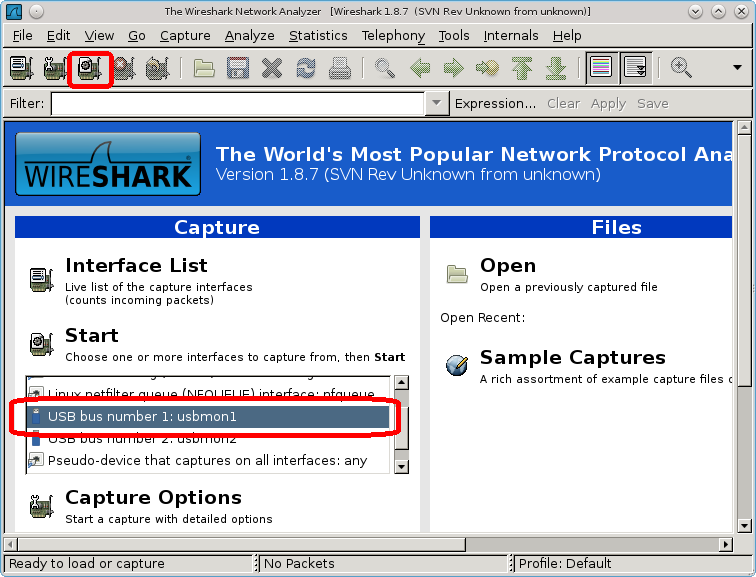
\includegraphics[width=10cm]{12_wireshark.png}
\end{figure}

Для анализа протокола нам необходимо перехватить следующие части генерируемого траффика:

\begin{itemize}
  \item инициализация устройства
  \item начало выполнения какой"=либо функции
  \item окончание выполнения какой"=либо функции
  \item деинициализация устройства
\end{itemize}

Обычно данные части отделены по времени, т.к. инициировать выполнения функции устройством можно в произвольное время (например, подвинуть мышку, нажать кнопку на клавиатуре, начать захват видео с веб"=камеры и т.д.)

Как правило, изучаемые устройства делятся на два типа:

\begin{itemize}
  \item Register"=oriented устройства
  \item Message"=oriented устройства
\end{itemize}

Для первых в перехватываемых трансферах будет чётко прослеживаться следующая структура:

\begin{itemize}
  \item заголовок трансфера (например, размер в байтах)
  \item адрес регистра
  \item значение (несколько значений)
  \item хвост трансфера (например, контрольная сумма)
\end{itemize}

Данные устройства предоставляют некое адресное пространство, в которое мы можем производить запись/чтение с помощью определённых USB"=трансферов.

Пример данного трансфера мы видим на иллюстрации:

\begin{figure}[h!]
  \centering
  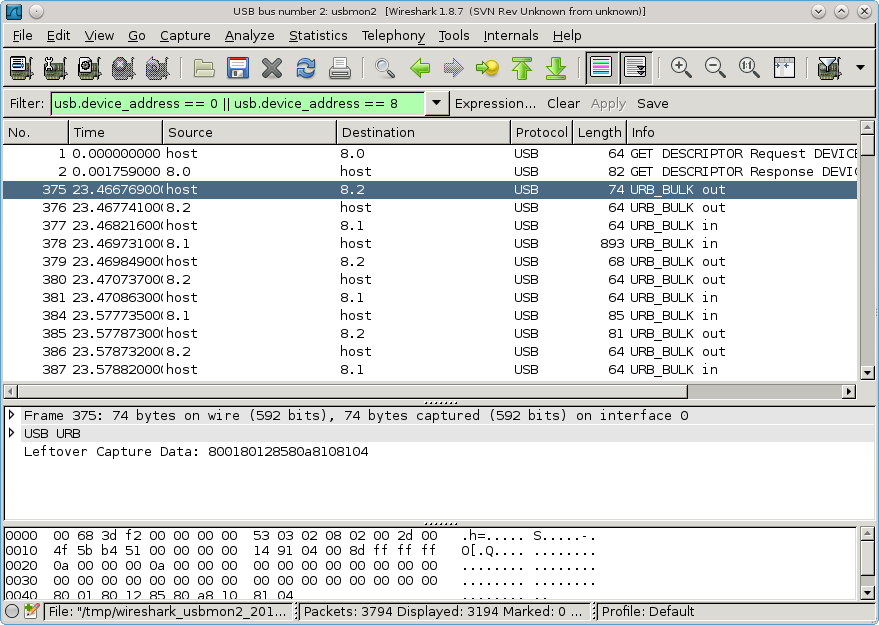
\includegraphics[width=10cm]{12_traffic-sample.png}
\end{figure}

См. трансфер \No 375, поле leftover capture data. В данном случае трансфер содержит пары адрес"=регистра "--- значение. Трансфер №376 является подтверждением, что устройство приняло трансфер. Трансфер \No 377 является запросом от хоста на приём данных от устройства, трансфер №378 "--- ответом устройства. Можно заметить, что любой трансфер в Wireshark виден как пара пакетов вида запрос хоста "--- ответ устройства (надеюсь, читатель еще помнить что все трансферы на USB шине инициирует хост?). Стоит отметить, что не всегда эта пара расположена линейно.

Для второго типа устройств в перехватываемых трансферах будет видна следующая структура:

\begin{itemize}
  \item заголовок трансфера
  \item тип сообщения
  \item тело сообщения
  \item хвост трансфера
\end{itemize}

Данные устройства, как правило, требуют больших усилий по расшифровке протокола.

Как правило, практически невозможно по дампу траффика, без экспериментов с устройством, расшифровать протокол. Для экспериментов удобно будет написать прототип драйвера с использованием библиотеки libusb. Данная библиотека работает в пространстве пользователя, т.о. при падении прототипа не упадёт вся ОС.

В качестве первого прототипа разумно будет повторить ту последовательность, которая записана в дампе. При запуске прототипа стоит записать еще один дамп, и сравнить его с оригинальным. Отличия между дампами сигнализируют о том, что что"=то прототип делает не так. Модификациями прототипа необходимо добиться идентичности дампа (в некоторых случаях это необязательно или невозможно, например при захвате картинки с камеры).

Пример простейших прототипов можно посмотреть в \cite{Anar4} и \cite{Anar5}. Как видно, эти прототипы состоят из следующих частей:

\begin{itemize}
  \item инициализация библиотеки: libusb\_init()
  \item открытие устройства: libusb\_open\_device\_with\_vid\_pid()
  \item выбор нужного интерфейса:  libusb\_claim\_interface()
  \item некоторого количества трансферов: libusb\_bulk\_transfer()/ \linebreak libusb\_control\_transfer()/libusb\_interrupt\_transfer()
  \item разбор ответа от устройства
  \item деинициализация: libusb\_close(); libusb\_exit()
\end{itemize}

\subsection*{Заключение}

Не смотря на то, что разбор протокола USB"=устройства кажется сложной задачей, на самом деле таковым не является "--- необходимо лишь упорство, терпение и желание экспериментировать.

\begin{thebibliography}{9}
\bibitem{Anar1} \url{http://www.beyondlogic.org/usbnutshell/usb1.shtml}
\bibitem{Anar2} \url{https://www.kernel.org/doc/Documentation/usb/usbmon.txt}
\bibitem{Anar3} \url{http://desowin.org/usbpcap/}
\bibitem{Anar4} \url{https://github.com/anarsoul/fprint\_aes1660}
\bibitem{Anar5} \url{https://github.com/anarsoul/fprint\_aes2550}
\end{thebibliography}

\end{document}





\documentclass[10pt, a5paper]{article}
\usepackage{pdfpages}
\usepackage{parallel}
\usepackage[T2A]{fontenc}
\usepackage{ucs}
\usepackage[utf8x]{inputenc}
\usepackage[polish,english,russian]{babel}
\usepackage{hyperref}
\usepackage{rotating}
\usepackage[inner=2cm,top=1.8cm,outer=2cm,bottom=2.3cm,nohead]{geometry}
\usepackage{listings}
\usepackage{graphicx}
\usepackage{wrapfig}
\usepackage{longtable}
\usepackage{indentfirst}
\usepackage{array}
\newcolumntype{P}[1]{>{\raggedright\arraybackslash}p{#1}}
\frenchspacing
\usepackage{fixltx2e} %text sub- and superscripts
\usepackage{icomma} % коскі ў матэматычным рэжыме
\PreloadUnicodePage{4}

\newcommand{\longpage}{\enlargethispage{\baselineskip}}
\newcommand{\shortpage}{\enlargethispage{-\baselineskip}}

\def\switchlang#1{\expandafter\csname switchlang#1\endcsname}
\def\switchlangbe{
\let\saverefname=\refname%
\def\refname{Літаратура}%
\def\figurename{Іл.}%
}
\def\switchlangen{
\let\saverefname=\refname%
\def\refname{References}%
\def\figurename{Fig.}%
}
\def\switchlangru{
\let\saverefname=\refname%
\let\savefigurename=\figurename%
\def\refname{Литература}%
\def\figurename{Рис.}%
}

\hyphenation{admi-ni-stra-tive}
\hyphenation{ex-pe-ri-ence}
\hyphenation{fle-xi-bi-li-ty}
\hyphenation{Py-thon}
\hyphenation{ma-the-ma-ti-cal}
\hyphenation{re-ported}
\hyphenation{imp-le-menta-tions}
\hyphenation{pro-vides}
\hyphenation{en-gi-neering}
\hyphenation{com-pa-ti-bi-li-ty}
\hyphenation{im-pos-sible}
\hyphenation{desk-top}
\hyphenation{elec-tro-nic}
\hyphenation{com-pa-ny}
\hyphenation{de-ve-lop-ment}
\hyphenation{de-ve-loping}
\hyphenation{de-ve-lop}
\hyphenation{da-ta-ba-se}
\hyphenation{plat-forms}
\hyphenation{or-ga-ni-za-tion}
\hyphenation{pro-gramming}
\hyphenation{in-stru-ments}
\hyphenation{Li-nux}
\hyphenation{sour-ce}
\hyphenation{en-vi-ron-ment}
\hyphenation{Te-le-pathy}
\hyphenation{Li-nux-ov-ka}
\hyphenation{Open-BSD}
\hyphenation{Free-BSD}
\hyphenation{men-ti-on-ed}
\hyphenation{app-li-ca-tion}

\def\progref!#1!{\texttt{#1}}
\renewcommand{\arraystretch}{2} %Іначай формулы ў матрыцы зліпаюцца з лініямі
\usepackage{array}

\def\interview #1 (#2), #3, #4, #5\par{

\section[#1, #3, #4]{#1 -- #3, #4}
\def\qname{LVEE}
\def\aname{#1}
\def\q ##1\par{{\noindent \bf \qname: ##1 }\par}
\def\a{{\noindent \bf \aname: } \def\qname{L}\def\aname{#2}}
}

\def\interview* #1 (#2), #3, #4, #5\par{

\section*{#1\\{\small\rm #3, #4. #5}}

\def\qname{LVEE}
\def\aname{#1}
\def\q ##1\par{{\noindent \bf \qname: ##1 }\par}
\def\a{{\noindent \bf \aname: } \def\qname{L}\def\aname{#2}}
}


\begin{document}

\title{Играем взводом или многополозовательские компьютерные системы на базе ОС Linux с поддержкой аппаратного ускорения 3D}

\author{Денис Пынькин\footnote{Минск, Беларусь; \url{Denis_Pynkin@epam.com}}}
\maketitle

\begin{abstract}
	Modern Linux-based distributions are extremely flexible and configurable, so a number of different approaches available on how to setup and use MultiSeat feature. The main idea is to share desktop computer among multiple family members without additional cost and to have a possibility to work or play for some people in the same time.
\end{abstract}

\subsection*{Linux --- современная игровая платформа}

За последний год произошло множество изменений и громких анонсов, которые позволяют
утверждать, что ОС Linux всерьез рассматривается в качестве платформы для запуска 
современных игровых продуктов. 
В проекте Humble Bundle часто фигурируют игры с поддержкой Linux; новые проекты Kickstarter
собирают необходимые суммы на разработку полноценных версий игр для Linux; Valve не только заявила
об официальной поддержке, но и создает игровую консоль на базе ОС Linux.
Не стоит забывать о проекте Wine и его интерфейсов управления, таких как PlayOnLinux --- множество 
программ рассчитанных на работу в альтернативных коммерческих ОС зачастую работают не хуже 
при запуске с помощью Wine, особенно это касается <<устаревших>> программ.
Ну и наконец, нельзя обойти стороной такое явление, как MMO --- нмногопользовательские онлайн"=игры,
в частности World of Tanks и War Thunder, благодаря которым появилась данная статья. 

\subsection*{Домашний компьютер --- поле боя за машинные ресурсы}

По мере взросления дети начинают играть в те же игры, что и родители. 
Первые тревожные звоночки появляются со словами: <<Папа, моя очередь играть в танчики>>,
где вместо <<танчиков>> может быть любая другая требовательная к 3D игра.

Наличие персональных ноутбуков не решает проблемы разделения игровых ресурсов --- ведь
многие мобильные устройства не обладают должной производительностью. 
Покупка отдельного игрового компьютера --- сомнительное и сравнительно дорогое удовольствие, 
не говоря уж об увеличении количества проводов в квартире.

Решением может быть использование Linux-системы в режиме MultiSeat (часто встречается, как 
<<Змей Горыныч>> в русскоязычных источниках): система с одним системным блоком и несколькими 
комплектами устройств ввода-вывода --- монитор-видеокарта-клавиатура-мышь.
Кроме того такая конфигурация может использоваться и в более классическом режиме для организации одного рабочего места с несколькими мониторами.

%\includegraphics[width=1in]{13_multiseat}

В качестве экпериментального стенда использовался далеко не новый компьютер на базе AMD Phenom 8450
с 4 GB оперативной памяти и 2-мя видеокартами на базе NVidia (GTX 650 и GT 440).

\subsection*{Технологии и конфигурации}

В отличие от некоторых коммерческих операционных систем, графический сервер Xorg и его производные
отлично приспособлены для работы в многоместном режиме.
Поэтому главная задача --- это запустить несколько экземпляров Xorg и не запутаться при этом, 
с каким из них необходимо ассоциировать устройства ввода.

Как показали эксперименты, для игр на базе Wine удобно использовать PlayOnLinux, который запускается
вместо Window \linebreak Manager сразу после графического входа --- это упрощает запуск для неопытных
пользователей. Наиболее оптимально для этого завести специальный <<игровой>> логин в системе. 
Кроме того в этом случае зачастую можно использовать один и тот же экземпляр игры, но в 
разных окружениях-контейнерах, что сэкономит десятки гигабайт дискового пространства и 
увеличит эффективность работы дискового кэша.

Еще одна проблема совершенно неожиданного свойства --- зачастую программы запускаемые в wine 
неоптимально используют ресурсы процессора. На самом деле в ряде экспериментов две игры использовали
одно ядро из трех доступных, совершенно игнорируя оставшиеся ядра процессора. Такое поведение 
напомнило, что при совместном использовании одной системы нужно делиться ресурсами, ну а раз
самостоятельно программы не уживаются, то можно это сделать насильно, при помощи механизма
Control Groups ядра Linux и {\tt cpuset} в частности.

\subsubsection*{Xorg и Display Manager}

Задача этой пары --- правильный запуск графического сервера.

В первую очередь необходимо создать конфигурации рабочих мест, для чего используется 
различные конфигурации \linebreak <<ServerLayout>>, для каждого из которых назначается в эксклюзивном режиме
одна видеокарта, а в секции <<Device>> указывается конкретное устройство с помощью <<BusID>>,
а опцией <<ProbeAllGpus>> отключается автоматический поиск других GPU.

Со стороны DM необходимо указать какому рабочему месту соответствует текущий графический сервер, 
например в KDM для этого в секции {\tt [X-:0-Core]} (для :0)  достаточно добавить имя конфигурации 
с использованием опции {\tt -layout} в командной строке вызова графического сервера.

Еще однин вариант работы X сервера --- мультидисплейный в режиме xinerama, когда к каждому выходу
видеокарты подключен монитор, а X сервер формирует общую картинку.

\subsubsection*{Устройства ввода}

По умолчанию все устройства ввода, такие как мышь и клавиатура, назначаются всем графическим серверам
одновременно. Поэтому в первую очередь необходимо правильно назначить соответствующую пару.
Сделать это можно с помощью механизма фильтрации устройств ввода в секции <<InputClass>>, 
опять-таки различными способами:
\begin{itemize}
	\item добавления тэга в правилах udev для устройства и подключения 
		только к соответствующему графическому серверу;
	\item добавить устройства не относящиеся к данному серверу в список игнориуемых.
\end{itemize}

Так как устройства ввода ассоциированы с соответствующим X сервером, а точнее <<ServerLayout>>, 
то в режиме xinerama нет возможности организовать отдельное рабочее место для каждого монитора.

\subsubsection*{Xephyr}

Xephyr \cite{Xephyr} --- это специальный X сервер, работающий в окне уже существующего X сервера.

Соответственно, если на одной видеокарте запустить X сервер в режиме xinerama, а затем поверх
запустить Xephyr по числу сконфигурированных выходов, то можно получить многопользовательскую
систему даже с помощью одной видеокарты. 
С ограничениями и без 3D поддержки, что на первый взгляд делает его бесполезным для данной статьи.

\subsubsection*{VirtualGL}

Проект VirtualGL \cite{VGL} выступает в роли своеобразного прокси для потоков команд OpenGL.
Работает как по сети, так и в локальном режиме, позволяя программам совместно использовать
ресурсы одного GPU.

В свою очередь запуск программ в Xephyr с использованием VirtualGL позволяет организовать 
столько рабочих мест с аппаратной поддержкой 3D, сколько существует аппаратных видеовыходов 
в компьютере!

Так с использованием компьютерной системы, описанной выше, теоретически можно организовать
6 рабочих мест, но на практике проверялись только 4 --- в доме просто не оказалось 
достаточного количества мониторов, клавиатур и мышей для проверки.

\subsubsection*{Звуковая подсистема}

В случае игр зачастую достаточно использования звукового сервера в режиме смешивания и вывода 
звука через одно устройство. Однако при наличии дополнительных звуковых карт, а современные 
видеокарты с поддержкой HDMI рассматриваются как пара GPU + звук, с помощью PulseAudio 
можно назначать отдельным программам вывод на различные звуковые карты \cite{MS2}.

\subsubsection*{logind}

Сервер {\tt logind} (часть systemd) изначально разрабатывался с учетом потребностей MultiSeat-конфигураций 
\cite{MS3}. Так в нем присутствует специальная сущность {\tt seat}, которая объединяет
сессию пользователя и программно-аппаратные ресурсы ассоциированные с этой сессией.

Для корректной работы с logind, необходима поддержка со стороны графического и оконного менеджеров,
которая, к сожалению, на момент подготовки тезисов была еще очень сырая,
а местами и просто нерабачая.

\subsection*{Области применения}

С учетом комбинирования различных технологий создавать многопользовательские системы можно (и нужно!)
под свои задачи --- кому-то хочется совместно поиграть, а кому-то достаточно минимальной аппаратной 
поддержки, но существенна стоимость каждого рабочего места.

Наиболее очевидные области применения:

\begin{itemize}
	\item Семейные игровые и рабочие системы
	\item Учреждения образования
	\item Игровые клубы
	\item Интернет-клубы
\end{itemize}

Отдельно стоит заметить, что такое использование мощностей видеокарты отлично
подходит для работы нескольких пользователей с коммерческими 3D-редакторами и CAD-системами,
которые ограничены лицензиями и привязкой к аппаратной конфигурации.

Ну а автор наслаждается MMO играя в одной команде вместе с подрастающим поколением,
так что теперь вместо фразы: <<Папа, моя очередь играть в танчики>>, теперь можно 
услышать: <<Папа, а давай поиграем в танчики вместе>>.


%=========================
\begin{thebibliography}{9}

\bibitem{MS1} ArchLinux: Xorg multiseat.
\url{https://wiki.archlinux.org/index.php/Xorg_multiseat}

\bibitem{MS2} Gentoo: Multiseat.
\url{http://wiki.gentoo.org/wiki/Multiseat#PulseAudio}


\bibitem{MS3} freedesktop.org: Multi-Seat on Linux
\url{http://www.freedesktop.org/wiki/Software/systemd/multiseat/}

\bibitem{VGL} The VirtualGL project
\url{http://www.virtualgl.org/}

\bibitem{Xephyr} freedesktop.org: Xephyr
\url{http://www.freedesktop.org/wiki/Software/Xephyr/}

\end{thebibliography}

\end{document}




 
\documentclass[10pt, a5paper]{article}
\usepackage{pdfpages}
\usepackage{parallel}
\usepackage[T2A]{fontenc}
\usepackage{ucs}
\usepackage[utf8x]{inputenc}
\usepackage[polish,english,russian]{babel}
\usepackage{hyperref}
\usepackage{rotating}
\usepackage[inner=2cm,top=1.8cm,outer=2cm,bottom=2.3cm,nohead]{geometry}
\usepackage{listings}
\usepackage{graphicx}
\usepackage{wrapfig}
\usepackage{longtable}
\usepackage{indentfirst}
\usepackage{array}
\newcolumntype{P}[1]{>{\raggedright\arraybackslash}p{#1}}
\frenchspacing
\usepackage{fixltx2e} %text sub- and superscripts
\usepackage{icomma} % коскі ў матэматычным рэжыме
\PreloadUnicodePage{4}

\newcommand{\longpage}{\enlargethispage{\baselineskip}}
\newcommand{\shortpage}{\enlargethispage{-\baselineskip}}

\def\switchlang#1{\expandafter\csname switchlang#1\endcsname}
\def\switchlangbe{
\let\saverefname=\refname%
\def\refname{Літаратура}%
\def\figurename{Іл.}%
}
\def\switchlangen{
\let\saverefname=\refname%
\def\refname{References}%
\def\figurename{Fig.}%
}
\def\switchlangru{
\let\saverefname=\refname%
\let\savefigurename=\figurename%
\def\refname{Литература}%
\def\figurename{Рис.}%
}

\hyphenation{admi-ni-stra-tive}
\hyphenation{ex-pe-ri-ence}
\hyphenation{fle-xi-bi-li-ty}
\hyphenation{Py-thon}
\hyphenation{ma-the-ma-ti-cal}
\hyphenation{re-ported}
\hyphenation{imp-le-menta-tions}
\hyphenation{pro-vides}
\hyphenation{en-gi-neering}
\hyphenation{com-pa-ti-bi-li-ty}
\hyphenation{im-pos-sible}
\hyphenation{desk-top}
\hyphenation{elec-tro-nic}
\hyphenation{com-pa-ny}
\hyphenation{de-ve-lop-ment}
\hyphenation{de-ve-loping}
\hyphenation{de-ve-lop}
\hyphenation{da-ta-ba-se}
\hyphenation{plat-forms}
\hyphenation{or-ga-ni-za-tion}
\hyphenation{pro-gramming}
\hyphenation{in-stru-ments}
\hyphenation{Li-nux}
\hyphenation{sour-ce}
\hyphenation{en-vi-ron-ment}
\hyphenation{Te-le-pathy}
\hyphenation{Li-nux-ov-ka}
\hyphenation{Open-BSD}
\hyphenation{Free-BSD}
\hyphenation{men-ti-on-ed}
\hyphenation{app-li-ca-tion}

\def\progref!#1!{\texttt{#1}}
\renewcommand{\arraystretch}{2} %Іначай формулы ў матрыцы зліпаюцца з лініямі
\usepackage{array}

\def\interview #1 (#2), #3, #4, #5\par{

\section[#1, #3, #4]{#1 -- #3, #4}
\def\qname{LVEE}
\def\aname{#1}
\def\q ##1\par{{\noindent \bf \qname: ##1 }\par}
\def\a{{\noindent \bf \aname: } \def\qname{L}\def\aname{#2}}
}

\def\interview* #1 (#2), #3, #4, #5\par{

\section*{#1\\{\small\rm #3, #4. #5}}

\def\qname{LVEE}
\def\aname{#1}
\def\q ##1\par{{\noindent \bf \qname: ##1 }\par}
\def\a{{\noindent \bf \aname: } \def\qname{L}\def\aname{#2}}
}


\begin{document}

\title{<<Долгоиграющие>> базы данных PostgreSQL}%\footnote{Текст данных и последующих тезисов, кроме специально оговоренных случаев, доступен под лицензией Creative Commons Attribution"=ShareAlike 3.0}

\author{Юрий Бушмелев\footnote{Ульяновск, Россия; \url{jay4mail@gmail.com}}}
\maketitle

\begin{abstract}
Big PostgreSQL databases under heavy load require special care. Database administrator should keep eye on amount of\linebreak indexes and tables bloat and use special tools to reduce bloat level. Big databases need extra handling when doing backup as well. Replication management is another special task. This talk describe some solutions how to deal with such databases in production.
\end{abstract}

Когда базы PostgreSQL вырастают до сотен гигабайт, обеспечение их бесперебойной и быстрой работы под высокими нагрузками начинает требовать особых подходов.

Длительный срок эксплуатации при постоянной записи в БД порождает проблему «распухания» индексов и таблиц. Необходимо уметь оценивать степень «опухания», чтобы своевременно проводить обслуживание таблиц и индексов. Для оценки можно использовать запросы, приведенные в wiki\cite{Bush1} или в презентации Michael Glaesemann\cite{Bush2}.

«Распухшие» индексы можно пересоздать штатной конструкцией SQL REINDEX, но это заблокирует таблицу на запись на время пересоздания индекса. Более «либеральный» вариант "--- создать аналогичный индекс конструкцией CREATE INDEX\linebreak CONCURRENTLY, затем удалить старый индекс и переименовать новый.

Для «компактизации» таблиц можно использовать конструкции VACUUM FULL и CLUSTER, но они также блокируют обрабатываемые таблицы. Поэтому были созданы альтернативные инструменты: vacuum\_table.pl \cite{Bush3} /pgcompactor \cite{Bush4} и pg\_repack \cite{Bush5}.

Большой объем БД и постоянная нагрузка создают проблемы с резервным копированием. Здесь нужно соблюсти баланс между длительностью резервного копирования, создаваемой им нагрузкой на сервер БД и занимаемым им объемом. Самый простой способ "--- создать дамп базы с помощью pg\_dump, но он использует конструкцию COPY, которая блокирует таблицы, и создает нагрузку на сервер БД. Альтернативный вариант "--- копирование кластера БД с файловой системы и сохранение WAL-логов. Более интересный вариант "--- использование снапшотов ФС и сохранение WAL-логов. Также есть специализированные решения "--- pg\_rman \cite{Bush6} и WAL-E \cite{Bush7}.

Необходимость постоянной доступности БД требует включения репликации, что также определяет некоторые особенности в обращении с базами. 
Для создания потоковой реплики можно использовать как обычные средства сетевого копирования (scp и rsync), так и специализированные утилиты "--- pg\_basebackup и repmgr \cite{Bush8}.

Переключение ролей по описанному в руководстве способу (с использованием trigger\_file) приводит к необходимости пересоздания подчиненных реплик, что выливается в затраты времени и трафика. Если есть возможность последовательного перезапуска всех узлов кластера репликации, то можно просто переконфигурировать узлы в новую схему и перезапустить их с новыми ролями.

Каждое из решений обозначенных выше проблем имеет как свои плюсы, так и свои минусы. Выбор решений зависит от требований и возможностей каждой конкретной инфраструктуры.

\begin{thebibliography}{9}
\bibitem{Bush1}\url{http://wiki.postgresql.org/wiki/Show\_database\_bloat}
\bibitem{Bush2}\url{http://www.pgcon.org/2009/schedule/attachments/96\_visualizing-postgres-2009-05-21.pdf}
\bibitem{Bush3}\url{http://code.google.com/p/compacttable/}
\bibitem{Bush4}\url{http://code.google.com/p/pgtoolkit/}
\bibitem{Bush5}\url{https://github.com/reorg/pg\_repack}
\bibitem{Bush6}\url{http://code.google.com/p/pg-rman/}
\bibitem{Bush7}\url{https://github.com/heroku/WAL-E}
\bibitem{Bush8}\url{http://www.repmgr.org/}
\end{thebibliography}
\end{document}





\documentclass[10pt, a5paper]{article}
\usepackage{pdfpages}
\usepackage{parallel}
\usepackage[T2A]{fontenc}
\usepackage{ucs}
\usepackage[utf8x]{inputenc}
\usepackage[polish,english,russian]{babel}
\usepackage{hyperref}
\usepackage{rotating}
\usepackage[inner=2cm,top=1.8cm,outer=2cm,bottom=2.3cm,nohead]{geometry}
\usepackage{listings}
\usepackage{graphicx}
\usepackage{wrapfig}
\usepackage{longtable}
\usepackage{indentfirst}
\usepackage{array}
\newcolumntype{P}[1]{>{\raggedright\arraybackslash}p{#1}}
\frenchspacing
\usepackage{fixltx2e} %text sub- and superscripts
\usepackage{icomma} % коскі ў матэматычным рэжыме
\PreloadUnicodePage{4}

\newcommand{\longpage}{\enlargethispage{\baselineskip}}
\newcommand{\shortpage}{\enlargethispage{-\baselineskip}}

\def\switchlang#1{\expandafter\csname switchlang#1\endcsname}
\def\switchlangbe{
\let\saverefname=\refname%
\def\refname{Літаратура}%
\def\figurename{Іл.}%
}
\def\switchlangen{
\let\saverefname=\refname%
\def\refname{References}%
\def\figurename{Fig.}%
}
\def\switchlangru{
\let\saverefname=\refname%
\let\savefigurename=\figurename%
\def\refname{Литература}%
\def\figurename{Рис.}%
}

\hyphenation{admi-ni-stra-tive}
\hyphenation{ex-pe-ri-ence}
\hyphenation{fle-xi-bi-li-ty}
\hyphenation{Py-thon}
\hyphenation{ma-the-ma-ti-cal}
\hyphenation{re-ported}
\hyphenation{imp-le-menta-tions}
\hyphenation{pro-vides}
\hyphenation{en-gi-neering}
\hyphenation{com-pa-ti-bi-li-ty}
\hyphenation{im-pos-sible}
\hyphenation{desk-top}
\hyphenation{elec-tro-nic}
\hyphenation{com-pa-ny}
\hyphenation{de-ve-lop-ment}
\hyphenation{de-ve-loping}
\hyphenation{de-ve-lop}
\hyphenation{da-ta-ba-se}
\hyphenation{plat-forms}
\hyphenation{or-ga-ni-za-tion}
\hyphenation{pro-gramming}
\hyphenation{in-stru-ments}
\hyphenation{Li-nux}
\hyphenation{sour-ce}
\hyphenation{en-vi-ron-ment}
\hyphenation{Te-le-pathy}
\hyphenation{Li-nux-ov-ka}
\hyphenation{Open-BSD}
\hyphenation{Free-BSD}
\hyphenation{men-ti-on-ed}
\hyphenation{app-li-ca-tion}

\def\progref!#1!{\texttt{#1}}
\renewcommand{\arraystretch}{2} %Іначай формулы ў матрыцы зліпаюцца з лініямі
\usepackage{array}

\def\interview #1 (#2), #3, #4, #5\par{

\section[#1, #3, #4]{#1 -- #3, #4}
\def\qname{LVEE}
\def\aname{#1}
\def\q ##1\par{{\noindent \bf \qname: ##1 }\par}
\def\a{{\noindent \bf \aname: } \def\qname{L}\def\aname{#2}}
}

\def\interview* #1 (#2), #3, #4, #5\par{

\section*{#1\\{\small\rm #3, #4. #5}}

\def\qname{LVEE}
\def\aname{#1}
\def\q ##1\par{{\noindent \bf \qname: ##1 }\par}
\def\a{{\noindent \bf \aname: } \def\qname{L}\def\aname{#2}}
}


\begin{document}

\title{Подход к преподаванию десктопных и сетевых возможностей GNU/Linux в университете}%\footnote{Текст данных и последующих тезисов, кроме специально оговоренных случаев, доступен под лицензией Creative Commons Attribution"=ShareAlike 3.0}

\author{Алексей Городилов, Александра Кононова\footnote{Москва, г. Зеленоград, Россия; \url{kaverina@mail.ru}, \url{illinc@bk.ru}}}
\maketitle

\begin{abstract}
An approach to teaching GNU/Linux basics in university is proposed. This program is the result of refactoring of earlier courses taught at MIET. This course's aim is to provide a working knowledge of the operating system, so students could start to use GNU/Linux. This is in contrast with previous course, which lost connection to practice and which was too difficult. The new version proved to be successful as a popular elective course.
\end{abstract}
Курс, посвящённый GNU/Linux, существовал в МИЭТ в течение многих лет. Но в определённый момент сложилась ситуация, при которой этот курс стал крайне непопулярен у студентов. Кроме того, прослушавшие курс студенты оказывались плохо подготовленными к использованию GNU/Linux на практике. Стало очевидно, что данный курс требует существенной переработки и модернизации.

В состав старого курса входило изучение Bash и утилит Unix, таких, как grep, awk, vi. Кроме того, в курс входила разработка программ для Unix с использованием fork-exec.

Хотя теоретически это давало студентам глубокое понимание операционной системы, но на практике студенты, не знакомые с Unix ранее, не могли освоить работу в этой системе. Кроме того, курс совершенно не давал представления о практическом применении Unix или GNU/Linux.

Студентам приходилось изучать три новых языка программирования, а также несколько новых библиотек.  Студентам было непонятно, зачем нужно изучать этот инструментарий. Ответить на вопрос «зачем» можно было только теоретически. Такая сложность  старого курса приводила к тому, что более половины студентов, изучающих его, начинали к концу семестра списывать лабораторные работы. Этот признак непонятного и переусложнённого курса проявляется и в других дисциплинах.

Два года назад было решено полностью модернизировать данный курс. В разработанном нами варианте основная часть курса была посвящена изучению графического интерфейса и прикладных программ.

В состав курса были включены 4 лекции по 2 академических часа и 8 практических занятий по 4 академических часа. 
В курс вошли следующие практические занятия:

\begin{enumerate}
  \item Работа в графических средах KDE и GNOME, на котором студенты получают базовые навыки по работе с системой, такие как доступ и поиск файлов, запуск программ и настройка параметров системы.
  \item Восстановление системы после сбоев и зависаний программ, на котором изучаются способы восстановить работоспособность системы после сбоев различной степени тяжести, от зависания отдельной программы до отключения X-сервера.
  \item Офисные приложения "--- на этом занятии изучается работа в офисных приложениях, которые являются аналогами собственнических офисных приложений, изучаемых студентами в курсе базовой компьютерной подготовки.
  \item Графика: растровые, векторные и 3D-редакторы "--- на этом занятии студенты пробуют работать в gimp, inkscape и blender. Целью этого занятия является знакомство с возможностями редакторов, чтобы студенты могли решить, следует ли изучать эти программы далее.
  \item Работа со звуком: настройка звуковой подсистемы и использование звуковых и midi- редакторов "--- студентам предлагается самостоятельно подключить к компьютеру и настроить микрофон, динамики (наушники), а также midi-клавиатуру, отредактировать записанный звук в audacity, а также запустить jack и перенастроить вывод на него, что позволяет глубже понять работу звуковой подсистемы в ОС, и диагностировать проблемы, связанные с ней.
  \item Работа с интерфейсом командной строки "--- на этом занятии изучаются основы работы с bash, полезность чего уже не вызывает у студентов сомнений.
  \item Настройка сети в GNU/Linux, в том числе маршрутизации и брандмауэра "--- на этом занятии студенты настраивают подключение компьютера к сети, а также маршрутизацию для раздачи интернета другим компьютерам с помощью networkmanager, а также с помощью традиционных средств (ifconfig, iptables), и базовую настройку прокси-сервера squid.
  \item Установка ОС "--- студенты могут установить на виртуальную машину ОС Ubuntu, Fedora или любой другой дистрибутив по их выбору.
\end{enumerate}

Такой курс оказался более успешным. Изначально это подтверждалось только отзывами студентов, но, когда в МИЭТ была введена возможность выбирать курсы, обновлённый курс «Основы \linebreak GNU/Linux» выбрали более 80\% студентов соответствующих специальностей.


\end{document}





\documentclass[10pt, a5paper]{article}
\usepackage{pdfpages}
\usepackage{parallel}
\usepackage[T2A]{fontenc}
\usepackage{ucs}
\usepackage[utf8x]{inputenc}
\usepackage[polish,english,russian]{babel}
\usepackage{hyperref}
\usepackage{rotating}
\usepackage[inner=2cm,top=1.8cm,outer=2cm,bottom=2.3cm,nohead]{geometry}
\usepackage{listings}
\usepackage{graphicx}
\usepackage{wrapfig}
\usepackage{longtable}
\usepackage{indentfirst}
\usepackage{array}
\newcolumntype{P}[1]{>{\raggedright\arraybackslash}p{#1}}
\frenchspacing
\usepackage{fixltx2e} %text sub- and superscripts
\usepackage{icomma} % коскі ў матэматычным рэжыме
\PreloadUnicodePage{4}

\newcommand{\longpage}{\enlargethispage{\baselineskip}}
\newcommand{\shortpage}{\enlargethispage{-\baselineskip}}

\def\switchlang#1{\expandafter\csname switchlang#1\endcsname}
\def\switchlangbe{
\let\saverefname=\refname%
\def\refname{Літаратура}%
\def\figurename{Іл.}%
}
\def\switchlangen{
\let\saverefname=\refname%
\def\refname{References}%
\def\figurename{Fig.}%
}
\def\switchlangru{
\let\saverefname=\refname%
\let\savefigurename=\figurename%
\def\refname{Литература}%
\def\figurename{Рис.}%
}

\hyphenation{admi-ni-stra-tive}
\hyphenation{ex-pe-ri-ence}
\hyphenation{fle-xi-bi-li-ty}
\hyphenation{Py-thon}
\hyphenation{ma-the-ma-ti-cal}
\hyphenation{re-ported}
\hyphenation{imp-le-menta-tions}
\hyphenation{pro-vides}
\hyphenation{en-gi-neering}
\hyphenation{com-pa-ti-bi-li-ty}
\hyphenation{im-pos-sible}
\hyphenation{desk-top}
\hyphenation{elec-tro-nic}
\hyphenation{com-pa-ny}
\hyphenation{de-ve-lop-ment}
\hyphenation{de-ve-loping}
\hyphenation{de-ve-lop}
\hyphenation{da-ta-ba-se}
\hyphenation{plat-forms}
\hyphenation{or-ga-ni-za-tion}
\hyphenation{pro-gramming}
\hyphenation{in-stru-ments}
\hyphenation{Li-nux}
\hyphenation{sour-ce}
\hyphenation{en-vi-ron-ment}
\hyphenation{Te-le-pathy}
\hyphenation{Li-nux-ov-ka}
\hyphenation{Open-BSD}
\hyphenation{Free-BSD}
\hyphenation{men-ti-on-ed}
\hyphenation{app-li-ca-tion}

\def\progref!#1!{\texttt{#1}}
\renewcommand{\arraystretch}{2} %Іначай формулы ў матрыцы зліпаюцца з лініямі
\usepackage{array}

\def\interview #1 (#2), #3, #4, #5\par{

\section[#1, #3, #4]{#1 -- #3, #4}
\def\qname{LVEE}
\def\aname{#1}
\def\q ##1\par{{\noindent \bf \qname: ##1 }\par}
\def\a{{\noindent \bf \aname: } \def\qname{L}\def\aname{#2}}
}

\def\interview* #1 (#2), #3, #4, #5\par{

\section*{#1\\{\small\rm #3, #4. #5}}

\def\qname{LVEE}
\def\aname{#1}
\def\q ##1\par{{\noindent \bf \qname: ##1 }\par}
\def\a{{\noindent \bf \aname: } \def\qname{L}\def\aname{#2}}
}


\begin{document}

\title{Эра post-PC в ВУЗах}%\footnote{Текст данных и последующих тезисов, кроме специально оговоренных случаев, доступен под лицензией Creative Commons Attribution"=ShareAlike 3.0}

\author{Дмитро Ванькевич\footnote{Львов, Украина; \url{dvankevich@gmail.com}}}
\maketitle

\begin{abstract}
Prognoses of Post"=PC era coming are discussed and some real statistics, to determine features of future computer"=based \linebreak workflow in higher education institutions. The «bring"=your"=own"=device» concept is reviewed as a possible infrastructure \linebreak modernization approach.
\end{abstract}

Про наступление эры post"=PC говорят с конца 90"=х годов XX"=века. Ведущие идеологи ИТ того времени "--- Лу Герстнер, Ларри Эллисон, Стив Джобс "--- предрекали скорый закат традиционным ПК. Но уже в 2000"=х годах сторонники <<концепции PostPC>> не отрицали, что компьютеры в смысле вычислительных и управляющих устройств не исчезнут. Имелся в виду лишь конец эры персональных компьютеров, в их Wintel"=воплощении\cite{Vank1}, их доминирования как в смысле технологий, так и (в первую очередь!) в смысле рынка \cite{Vank2}.

Исследования Paul Marsden для конференции Digital Innovation Day 2013 подтверждает правоту предыдущего утверждения\cite{Vank3}. Если в 1998--2005 платформа Wintel доминировала (96\%), то на конец 2012 года её доля составила около 35\%. Будучи одним из ведущих производителей материнских плат, фирма Intel, заявила о прекращении выпуска этого вида продукции \cite{Vank4}. Но несмотря на снижение доли ПК среди всех вычислительных устройств, говорить про их уход с рынка ещё очень рано. Скорее всего произойдёт переопределение термина ПК. Так например на смену традиционным настольным ПК Intel предлагает <<Next Unit of Computing>> "--- ультракомпактный системный блок размером $12\times11\times4$ см на основе процессоров Core i3, i5 \cite{Vank5}.

Скорее можно утверждать, что эра post"=PC "--- это эра многообразия форм компьютерных систем, в которой произойдёт освобождение рабочего места от привязки к конкретному ПК, стоящему на столе. При помощи виртуализации десктопов возможно превратить рабочее место в виртуальное, доступное с любого клиентского устройства \cite{Vank6}.  Виртуализация рабочих мест позволит использовать концепцию BYOD (англ. «bring"=your"=own"=device» "--- «принеси собственное устройство»), которая получила широкое распространение в течение последних нескольких лет. Она подразуемевает использование студентами собственных клиентских устройств в учебных целях. К 2017 году, по прогнозу Gartner, каждый второй работник будет пользоваться собственными гаджетами в рабочих целях \cite{Vank7}. И уже сейчас большинство студентов ВУЗов имеют в своём распоряжении ноутбуки, которые по своим параметрам зачастую превосходят находящиеся в учебном классе ПК. Это стоит учитывать при построеннии ИТ инфраструктуры ВУЗа. В частности, учитывая характерный для вузов развитый компьютерный парк и достаточно мощное подразделение по его обслуживанию, имеет смысл вкладывать ресурсы не столько в обновление ПК, сколько в построение частного облака, предоставляющего студентам необходимые приложения в качестве сервисов.

При формировании комплекса сервисов для ВУЗовской сети и переносе локальных задач в частное облако просматриваются два подхода. Первый заключается в применении технологии web desktops "--- окружений рабочего стола, написанных на основе веб"=технологий (преимущественно, PHP), запускаемых на сервере и взаимодействующих с пользователем через веб"=браузер \cite{Vank8}. Преимуществом такого подхода является нетребовательность к ресурсам, а недостатком "--- ограниченные возможности существующих систем этого типа, в особенности распространяемых под свободными лицензиями. Т.о. подход может быть рекомендован к использованию только совместно с альтернативными решениями.

Альтернативой интранет"=технологиям является использование виртуализации. Помимо поднятия сервера виртуальных машин с нуля, для построения частного облака можно использовать одно из готовых решений. В частности, одно из таких решений "--- дистрибутив Proxmox Virtual Environment \cite{Vank9} \cite{Vank10} "--- успешно использовался для создания учебного полигона при проведении лабораторных работ в рамках курса <<Системное администрирование ОС Linux>> во Львовском национальном университете имени Ивана Франко\cite{Vank11}.



\begin{thebibliography}{9}
\bibitem{Vank1} Wintel "--- маркетинговый термин, сокращение, образованное слиянием слов Windows и Intel, которое обозначает персональный компьютер, использующий центральный процессор с x86"=совместимой микроархитектурой и операционную систему семейства Microsoft Windows. \url{http://ru.wikipedia.org/wiki/Wintel}
\bibitem{Vank2} <<Еще раз о PostPC>> журнал PC Magazine RE август 2000г. \url{http://www.pcmag.ru/issues/detail.php?ID=6682}
\bibitem{Vank3} <<Post"=PC Era by the Numbers: List of Top Post"=PC Stats>> \url{http://socialcommercetoday.com/post-pc-era-by-the-numbers-list-of-top-post-pc-stats/}
\bibitem{Vank4} <<Intel Will Exit Desktop Motherboard Market After Haswell is Released>> \url{http://www.legitreviews.com/news/14994/}
\bibitem{Vank5} <<Intel® NUC>> \url{http://www.intel.com/content/www/us/en/motherboards/desktop-motherboards/nuc.html}
\bibitem{Vank6} <<ПК умер "--- да здравствует ПК!>> «Открытые системы», № 09, 2011 \url{http://www.osp.ru/os/2011/09/13011556/}
\bibitem{Vank7} <<Gartner прогнозирует бум BYOD в 2016 году>> \url{http://www.therunet.com/news/905-gartner-prognoziruet-bum-byod-v-2016-godu}
\bibitem{Vank8} <<Web desktop>> \url{http://en.wikipedia.org/wiki/Web\_desktop}
\bibitem{Vank9} \url{http://pve.proxmox.com}
\bibitem{Vank10} Д.Є.Ванькевич, Г.Г.Злобін. Використання приватної хмари на базі дистрибутиву PROXMOXVE в навчальному процесі, Хмарні технології в освіті: матеріали Всеукраїнського науково"=методичного Інтернет"=семінару (Кривий Ріг "--- Київ "--- Черкаси "--- Харків, 21 грудня 2012р.). "--- Кривий Ріг: Видавничий відділ КМІ, 2012. "--- 173 с.
\bibitem{Vank11} Д.Є.Ванькевич. Навчальний полігон на базі дистрибутиву PROXMOXVE для проведення лабораторних робіт з курсу <<Системне адміністрування ОС LINUX>>, Теорія та методика електронного навчання: збірник наукових праць. Випуск IV. "--- Кривий Ріг: Видавничий відділ КМІ, 2013. "--- 311 с.
\end{thebibliography}
\end{document}





\documentclass[10pt, a5paper]{article}
\usepackage{pdfpages}
\usepackage{parallel}
\usepackage[T2A]{fontenc}
\usepackage{ucs}
\usepackage[utf8x]{inputenc}
\usepackage[polish,english,russian]{babel}
\usepackage{hyperref}
\usepackage{rotating}
\usepackage[inner=2cm,top=1.8cm,outer=2cm,bottom=2.3cm,nohead]{geometry}
\usepackage{listings}
\usepackage{graphicx}
\usepackage{wrapfig}
\usepackage{longtable}
\usepackage{indentfirst}
\usepackage{array}
\newcolumntype{P}[1]{>{\raggedright\arraybackslash}p{#1}}
\frenchspacing
\usepackage{fixltx2e} %text sub- and superscripts
\usepackage{icomma} % коскі ў матэматычным рэжыме
\PreloadUnicodePage{4}

\newcommand{\longpage}{\enlargethispage{\baselineskip}}
\newcommand{\shortpage}{\enlargethispage{-\baselineskip}}

\def\switchlang#1{\expandafter\csname switchlang#1\endcsname}
\def\switchlangbe{
\let\saverefname=\refname%
\def\refname{Літаратура}%
\def\figurename{Іл.}%
}
\def\switchlangen{
\let\saverefname=\refname%
\def\refname{References}%
\def\figurename{Fig.}%
}
\def\switchlangru{
\let\saverefname=\refname%
\let\savefigurename=\figurename%
\def\refname{Литература}%
\def\figurename{Рис.}%
}

\hyphenation{admi-ni-stra-tive}
\hyphenation{ex-pe-ri-ence}
\hyphenation{fle-xi-bi-li-ty}
\hyphenation{Py-thon}
\hyphenation{ma-the-ma-ti-cal}
\hyphenation{re-ported}
\hyphenation{imp-le-menta-tions}
\hyphenation{pro-vides}
\hyphenation{en-gi-neering}
\hyphenation{com-pa-ti-bi-li-ty}
\hyphenation{im-pos-sible}
\hyphenation{desk-top}
\hyphenation{elec-tro-nic}
\hyphenation{com-pa-ny}
\hyphenation{de-ve-lop-ment}
\hyphenation{de-ve-loping}
\hyphenation{de-ve-lop}
\hyphenation{da-ta-ba-se}
\hyphenation{plat-forms}
\hyphenation{or-ga-ni-za-tion}
\hyphenation{pro-gramming}
\hyphenation{in-stru-ments}
\hyphenation{Li-nux}
\hyphenation{sour-ce}
\hyphenation{en-vi-ron-ment}
\hyphenation{Te-le-pathy}
\hyphenation{Li-nux-ov-ka}
\hyphenation{Open-BSD}
\hyphenation{Free-BSD}
\hyphenation{men-ti-on-ed}
\hyphenation{app-li-ca-tion}

\def\progref!#1!{\texttt{#1}}
\renewcommand{\arraystretch}{2} %Іначай формулы ў матрыцы зліпаюцца з лініямі
\usepackage{array}

\def\interview #1 (#2), #3, #4, #5\par{

\section[#1, #3, #4]{#1 -- #3, #4}
\def\qname{LVEE}
\def\aname{#1}
\def\q ##1\par{{\noindent \bf \qname: ##1 }\par}
\def\a{{\noindent \bf \aname: } \def\qname{L}\def\aname{#2}}
}

\def\interview* #1 (#2), #3, #4, #5\par{

\section*{#1\\{\small\rm #3, #4. #5}}

\def\qname{LVEE}
\def\aname{#1}
\def\q ##1\par{{\noindent \bf \qname: ##1 }\par}
\def\a{{\noindent \bf \aname: } \def\qname{L}\def\aname{#2}}
}


\begin{document}

\title{Обзор реализаций поддержки мультиархитектур в дистрибутивах Linux и их сборочных системах}%\footnote{Текст данных и последующих тезисов, кроме специально оговоренных случаев, доступен под лицензией Creative Commons Attribution"=ShareAlike 3.0}

\author{Константин Шевцов\footnote{Минск, Беларусь; EPAM Systems; \url{int3g3r@gmail.com}}}
\maketitle

\begin{abstract}
The world is not ideal that's why some packages can't built under certain architecture (i.e. grub, wine) or some vendors doesn't produce packages (skype, steam). In future it will allow run ancient packages.
For this cases all distributives has multiarch support "--- installing of packages from more then one architecture in one system.
This article is an overview of multiarch realizations in modern GNU/Linux distributives: OpenSUSE, Fedora, Debian/Ubuntu, Gentoo, ArchLinux and describes differences in package lifecycle.
\end{abstract}

\begin{center}\end{center}

По мере появления новых архитектур компьютеров стали появляться дистрибутивы собранные под эти архитектуры. По ряду причин не все программы под GNU/Linux существуют и могут работать под родной архитектурой системы: так например wine и grub не могут быть собраны под архитектуру x86\_64, а некоторые закрытые программы, например skype и steam, поставляются собранные только под x86. Поэтому дистрибутивы начали приспосабливать свои пакетные менеджеры и сборочные системы. Способ совмещения пакетов двух разных архитектур в одной установке называется как multiarch или bi"=arch.

Рассмотрим как эта ситуация решается в ряде наиболее распространенных дистрибутивов. В качестве ярко выраженного примера рассмотрим сборку и установку gcc с поддержкой multilib (-m32 \& -m64 build flags) для x86\_64.

\subsubsection*{OpenSUSE}

Используемая в дистрибутиве сборочная система OBS \cite{Sha1} не позволяет устанавливать пакеты сторонних архитектур в сборочное окружение. Чтобы решить данную проблему создан механизм baselibs \cite{Sha2} --- перепакетировка содержимого пакета одной архитектуры в другую. Например, x86"=пакет с именем foo после сборки дублируется в foo"=32bit с архитектурой x86\_64 (модификация имени и архитектуры в метаинформации пакета). Далее такой пакет копируется в x86\_64"=репозиторий, и этот репозиторий целиком паблишится для пользования конечным пользователем. Пути размещения библиотек "--- /lib32 и /lib64. Дистрибутив использует пакетный менеджер rpm/zypper, а для расчета зависимостей применяется libsolv \cite{Sha3}.

\subsubsection*{Fedora}

Сборочная система Koji \cite{Sha4} также не позволяет смешивать архитектуры в buildroot'e. Для удовлетворения сборки x86\_64 multilib gcc, grub применяется спрятанный пакет"=заглушка glibc32 \cite{Sha5}, который содержит 32"=битные библиотеки. Файлы сборки (.spec) написаны так, чтобы при установке rpm"=пакеты библиотек и заголовочных файлов двух архитектур не конфликтовали в одной системе. Пакетный менеджер Yum понимает архитектуры <<pkgname.arch>>. Для конечного пользователя предоставляется один репозиторий, содержащий выборку пакетов из двух архитектур  (для паблишинга используется утилита mash \cite{Sha6}). Пути укладки библиотек "---  /lib32 и /lib64. Используется пакетный менеджер rpm/yum, а расчет зависимостей выполняется yum <<compare\_providers>> \cite{Sha7}. Существует также экспериментальный проект rpm/Hawkey/DNF с использованием libsolv.

\subsubsection*{Debian / Ubuntu}

В Debian до версии 7 и в Ubuntu до версии 11.04 картина выглядит следующим образом. Большие пакеты ia32-* \cite{Sha8} содержат x86"=библиотеки и имеют архитектуру x86\_64. Их неудобно поддерживать, типичен очень большой размер (порядка 33 МБ), а версия пакета обычно представляет собой дату сборки.

Начиная с версии 7 в Debian и версии 11.04 в Ubuntu добавлена поддержка различия архитектур установки <<pkgname:arch>> для dpkg/apt"=get. Сборка происходит в buildd, добавлено новое поле в сборочных файлах Multi"=arch. Но для сборки по"=прежнему используются  пакеты lib32*. Пути установки имеют вид prefix/lib/triplet (т.е. происходит игнорирование FHS). Пакетный менеджер по"=прежнему dpkg/apt"=get (или aptitude).

\subsubsection*{Gentoo}

В связи с тем, что это source"=based дистрибутив, в нем существует три различных способа решения рассматриваемой задачи\cite{Sha9}:

\begin{enumerate}
  \item Изначальный способ -- это большие пакеты emul-linux-* x86\_64 \cite{Sha10} содержащие файлы с архитектурой x86.
  \item Существует также проект gx86-multilib \cite{Sha11}c eclass'ами, которые добавляют архитектурные USE"=флаги (abi\_x86\_32, abi\_x86\_64), управляющие зависимостями. Использование этого подхода требует изменения текущих ebuild'ов, например wine \cite{Sha12}.
  \item Форк multilib"=portage позволяет собирать пакеты сразу под нужные архитектуры без модификации ebuild'ов.
\end{enumerate}

Во всех случаях используется пакетный менеджер portage.

\subsubsection*{ArchLinux}

Данный дистрибутив имеет отдельный репозиторий multilib \cite{Sha13}, в котором собираются пакеты с архитектурой x86\_64, именем пакета lib32-* и x86"=содержимым. Пакетный менеджер "--- pacman.

\subsubsection*{Выводы}

Таким образом видно, что у большинства дистрибутивов первым этапом поддержки мультиархитектур было простое добавление x86\_64"=пакетов с x86"=содержимым. Однако, наиболее правильным способом на данный момент видится вариант, когда содержимое пакета соответствует метаинформации пакета, а зависимости строятся с учетом архитектур, исключая конфликты путей. В дальнейшем такие улучшения должны помимо более корректного построения пакетной базы позволить миграцию между архитектурами без переустановки и возможность запуска <<древних>> программ старых архитектур в новых версиях дистрибутивов, что на текущий момент является актуальной и нерешенной проблемой.

\begin{thebibliography}{9}
\bibitem{Sha1} \url{https://build.opensuse.org/}
\bibitem{Sha2} \url{https://en.opensuse.org/openSUSE:Build\_Service\_baselibs.conf}
\bibitem{Sha3} \url{https://github.com/openSUSE/libsolv}
\bibitem{Sha4} \url{http://koji.fedoraproject.org/koji/}
\bibitem{Sha5} \url{https://lists.fedoraproject.org/pipermail/buildsys/2011-January/003496.html}
\bibitem{Sha6} \url{https://admin.fedoraproject.org/pkgdb/acls/name/mash}
\bibitem{Sha7} \url{http://yum.baseurl.org/wiki/CompareProviders}
\bibitem{Sha8} \url{http://packages.debian.org/squeeze/ia32-libs}
\bibitem{Sha9} \url{http://wiki.gentoo.org/wiki/Multilib}
\bibitem{Sha10} \url{http://www.gentoo.org/proj/en/base/amd64/emul/emul-linux-x86-20130224.xml}
\bibitem{Sha11} \url{http://wiki.gentoo.org/wiki/Gx86-multilib}
\bibitem{Sha12} \url{http://sources.gentoo.org/cgi-bin/viewvc.cgi/gentoo-x86/app-emulation/wine/wine-1.5.31.ebuild?view=markup\#33}
\bibitem{Sha13} \url{https://wiki.archlinux.org/index.php/Arch64\_FAQ\#Multilib\_Repository\_-\_Multilib\_Project}
\end{thebibliography}
\end{document}





\documentclass[10pt, a5paper]{article}
\usepackage{pdfpages}
\usepackage{parallel}
\usepackage[T2A]{fontenc}
\usepackage{ucs}
\usepackage[utf8x]{inputenc}
\usepackage[polish,english,russian]{babel}
\usepackage{hyperref}
\usepackage{rotating}
\usepackage[inner=2cm,top=1.8cm,outer=2cm,bottom=2.3cm,nohead]{geometry}
\usepackage{listings}
\usepackage{graphicx}
\usepackage{wrapfig}
\usepackage{longtable}
\usepackage{indentfirst}
\usepackage{array}
\newcolumntype{P}[1]{>{\raggedright\arraybackslash}p{#1}}
\frenchspacing
\usepackage{fixltx2e} %text sub- and superscripts
\usepackage{icomma} % коскі ў матэматычным рэжыме
\PreloadUnicodePage{4}

\newcommand{\longpage}{\enlargethispage{\baselineskip}}
\newcommand{\shortpage}{\enlargethispage{-\baselineskip}}

\def\switchlang#1{\expandafter\csname switchlang#1\endcsname}
\def\switchlangbe{
\let\saverefname=\refname%
\def\refname{Літаратура}%
\def\figurename{Іл.}%
}
\def\switchlangen{
\let\saverefname=\refname%
\def\refname{References}%
\def\figurename{Fig.}%
}
\def\switchlangru{
\let\saverefname=\refname%
\let\savefigurename=\figurename%
\def\refname{Литература}%
\def\figurename{Рис.}%
}

\hyphenation{admi-ni-stra-tive}
\hyphenation{ex-pe-ri-ence}
\hyphenation{fle-xi-bi-li-ty}
\hyphenation{Py-thon}
\hyphenation{ma-the-ma-ti-cal}
\hyphenation{re-ported}
\hyphenation{imp-le-menta-tions}
\hyphenation{pro-vides}
\hyphenation{en-gi-neering}
\hyphenation{com-pa-ti-bi-li-ty}
\hyphenation{im-pos-sible}
\hyphenation{desk-top}
\hyphenation{elec-tro-nic}
\hyphenation{com-pa-ny}
\hyphenation{de-ve-lop-ment}
\hyphenation{de-ve-loping}
\hyphenation{de-ve-lop}
\hyphenation{da-ta-ba-se}
\hyphenation{plat-forms}
\hyphenation{or-ga-ni-za-tion}
\hyphenation{pro-gramming}
\hyphenation{in-stru-ments}
\hyphenation{Li-nux}
\hyphenation{sour-ce}
\hyphenation{en-vi-ron-ment}
\hyphenation{Te-le-pathy}
\hyphenation{Li-nux-ov-ka}
\hyphenation{Open-BSD}
\hyphenation{Free-BSD}
\hyphenation{men-ti-on-ed}
\hyphenation{app-li-ca-tion}

\def\progref!#1!{\texttt{#1}}
\renewcommand{\arraystretch}{2} %Іначай формулы ў матрыцы зліпаюцца з лініямі
\usepackage{array}

\def\interview #1 (#2), #3, #4, #5\par{

\section[#1, #3, #4]{#1 -- #3, #4}
\def\qname{LVEE}
\def\aname{#1}
\def\q ##1\par{{\noindent \bf \qname: ##1 }\par}
\def\a{{\noindent \bf \aname: } \def\qname{L}\def\aname{#2}}
}

\def\interview* #1 (#2), #3, #4, #5\par{

\section*{#1\\{\small\rm #3, #4. #5}}

\def\qname{LVEE}
\def\aname{#1}
\def\q ##1\par{{\noindent \bf \qname: ##1 }\par}
\def\a{{\noindent \bf \aname: } \def\qname{L}\def\aname{#2}}
}


\begin{document}

\title{XMPP/Jabber глазами мантейнера jabber.org.by}%\footnote{Текст данных и последующих тезисов, кроме специально оговоренных случаев, доступен под лицензией Creative Commons Attribution"=ShareAlike 3.0}

\author{Влад Шахов\footnote{Лодзь, Польша; \url{lumpen.intellectual@gmail.com}}}
\maketitle

\begin{abstract}
Raise and fall of XMPP technology is analyzed as far as notes are given to the Second IM world war, including Google Talk abolish and protocols incompatibility hell. Brief history and current state of Jabber.org.by, the first public  Jabber/XMPP server in Belarus, is presented as an example of community"=driven XMPP project. 
\end{abstract}

\section{Технология XMPP/Jabber}

\subsection{Общие сведения}

Протокол \textbf{XMPP} (\textbf{Extensible Messaging and Presence Protocol} "--- \emph{расширяемый протокол обмена сообщениями и информацией о присутствии}). Основан на формате XML и изначально спроектирован расширяемым. Стандартизирован в настоящее время в RFC 6120, RFC 6121, и RFC 6122. Плюс расширения (XEP) от \url{http://xmpp.org}.

Существует огромное множество реализаций XMPP, клиентских и серверных, как общего назначения, так и специализированных.

Поддерживаются очевидные для Instant Messenging возможности передачи текстовых сообщений, групповых чатов, серверной истории, передачи голоса и видео, а также файлов.

Существенным отличием от многих других IM является децентрализованность. В XMPP адрес пользователя состоит из двух частей: login@server. Каждый сервер является независимой сущностью, которая договаривается о доставке сообщений с другими серверами посредством протокола XMPP. Этот процесс называется XMPP Federation или XMPP s2s.

\subsection{Наиболее интересные возможности XMPP}

\begin{itemize}
  \item серверные шлюзы (<<транспорты>>) в сети на других технологиях (ICQ, Skype, MSN, SIP, IRC, Email). Включая другие сервера на XMPP. Включая подписку на транспорты других серверов.
  \item Шифрование: канал клиент"=сервер и сервер"=сервер. Также можно шифровать отдельные сообщения открытым ключом.
  \item Удалённая передача команд и мониторинг состояния, в том числе управление клиентами и серверами XMPP.
  \item Инструменты совместной работы (Abiword, Inkscape, LibreOffice, Coccinella, всевозможные whiteboard).
  \item Микроблоггинг.
  \item Различные сетевые распределённые настольные игры.
  \item Геолокация.
  \item Сервисы идентификации : OpenID, OAuth.
  \item Облачные вычисления.
\end{itemize}

\section{XMPP vs. другие IM}

\subsection{Подъём и, одновременно, падение XMPP.}

На настоящий момент технология  XMPP очевидно устоялась и заняла свои позиции на рынке. Многие популярные интернет сервисы имеют XMPP на борту, в частности Facebook, GTalk, Vkontakte, WhatApp. Большинство бизнес"=ориентированных решений или имеют транспорты для подключения к XMPP Federation (Microsft Lync, Cisco Unified Presence), или прямо основаны на XMPP.

С другой стороны, большинство разработчиков корпоративных и открытых решений делает продукты под себя.  Выбрасывая или обрезая штатный функционал протокола и широко распространённые расширения.

С серверной стороны "--- зачастую мы можем видеть отключение s2s (Facebook), невозможность поменять личные данные через VCard (почти все), странное нестандартное поведение аккаунтов и серверов (Google Talk), отключенной server"=side history, нет поддержки групп  и т.д.

С клиентской "--- нет поддержки Service Discovery (imo, im+, xabber), и связанной с ней регистрации на транспортах и выполнения команд, нет поддержки конференций, а иногда даже групп пользователей в ростере (imo). Особенно этим грешат многопротокольные клиенты, где XMPP лишь одна из опций.

Суммируем "--- теоретическое богатство возможностей XMPP, описанных в предыдущем пункте, недоступно в коробочном, простом для использования, продукте. Требует дополнительных ощутимых усилий со стороны оператора сервера и конечного пользователя по настройке окружения.

Таким образом, мы можем смело говорить об протоколах, расширениях  и програмном обеспечении XMPP как о наборе заготовок <<сделай сам>>.

\subsection{Заметки о Первой и Второй Великой Войне среди IM's.}

Первая Великая Война IM началась после взлёта ICQ в конце 90х. Ключевым функционалом того времени являлась передача текста и групповые чаты.  В короткое время были созданы конкурирующие продукты: AIM, Yahoo Messenger, MSN и другие, мало отличающиеся функционалом, но абсолютно несовместимые друг с другом и обладающие закрытыми двоичными протоколами.

Со стороны пользователей практически сразу возник спрос на интеграцию множества несовместимых аккаунтов в одну точку входа.

Сформировалось 2 магистральных подхода:

\begin{enumerate}
  \item Многопротокольные клиенты. Примеры Miranda, Gaim/Pidgin, Trillian, Empathy/Telepathy.
  \item Сервер выступает в роли интегратора, клиент работает по одному протоколу. Примеры: XMPP, MS Lync, Cisco Unified Meeting Place, IMO.
\end{enumerate}

К середине 2000х все  протоколы IM подверглись реверс"=инженерингу, и к ним были написаны реализации XMPP"=транспортов, что позволило использовать свой XMPP"=аккаунт как единую точку входа во все сети, а особенности реализации маскировались.

Вторая Великая Война IM началась после повсеместного внедрения широкополосного доступа в интернет и появившейся возможностью передавать звук (VoIP) и видео. Чуть позже появилась и разрослась ниша мобильных устройств, планшетов и связанные с ними новые операционные системы. Традиционные участники рынка,  с трудом пережившие 1"=ю войну IM, не смогли оперативно среагировать и начался взлёт новых игроков, таких как Skype.

Мы видим снова ту же ситуацию, что и 10 лет назад. Коммерческие вендоры, стремясь наглухо привязать пользователей исключительно к своим сервисам, снова активно выбрасывают на рынок и продвигают полностью закрытые решения, зачастую не имеющие даже внешнего API. В частности отдельным недобрым словом можно отметить Skype, Viber, WhatsApp.  Отмечу однако, что в настоящий момент есть минимум 2 стандартизированных стека протоколов, SIP и XMPP, которые позволили бы обеспечить совместимость решений.  Но вендоры указанных сервисов в совместимости категорически не заинтересованы.

Уже сейчас появились признаки того, что конец 2"=й мировой войны IM будет таким же, как и для первой. Рынок поделят несколько коммерческих решений. Их  протоколы чуть позднее пройдут Reverse Engineering и будут реализованы в СПО как библиотеки. Библиотеки будут подключены  к многопротокольным клиентам и XMPP"=транспортам.

\subsection{Проприеритарные игры в открытый XMPP на примере Facebook.}

Согласно утечкам информации "--- архитектура чата Facebook вообще не основана на XMPP. XMPP"=gate написан дополнительно и имеет предельно ограниченный функционал.

Facebook via XMPP, текущий статус.
есть:

\begin{itemize}
  \item чат с пользователями в Facebook
  \item их статус онлайн/оффлайн
  \item поддерживает несколько соединений одновременно
\end{itemize}

нет:

\begin{itemize}
  \item S2S
  \item сервисов и транспортов
  \item групп и управления группами
  \item видео и аудио
  \item не работает VCard (нельзя публиковать и просмотреть, у пользователей только имя)
  \item запутанная схема подключения
  \item нельзя публиковать материалы в ленту
  \item нельзя подключать новых пользователей
  \item нельзя читать ленту
\end{itemize}

Вывод "--- годится только для подключения через J2J транспорт к вашему основному Jabber"=аккаунту.

\subsection{Былинный отказ Google Talk.}

Попробуем выделить из PR"=шума на тему отказа Google от XMPP факты.

От старта в  2006 и к маю 2013 Google Talk стал крупнейшим сервером XMPP, поддерживающим XMPP Federation. Такой результат мог быть достигнут только за счёт навязывания Google Talk в нагрузку к GMail, Android и другим популярным продуктам компании.  Голос, видео и звонки на телефонные сети в GTalk появились позже чем в Skype, более того их реализация сейчас мало совместима с остальным XMPP. Т.к. стандарт Jingle 1.0, разработанный по мотивам реализации Google Jingle 0.9 "--- сам Google не внедрил.

Google не замечен в активной работе над стандартами XMPP (RFC и XEP) кроме Jingle, выпуске клиентских или серверных реализаций под свободными лицензиями. Также серверная реализация GTalk имеет ряд неприятных особенностей, вынуждающие авторов решений на XMPP вставлять костыли на @gmail.com в свои продукты.

Из ощутимого вклада в развитие XMPP можем отметить только:

\begin{itemize}
  \item публикацию libjingle (voice, video, streaming, file sharing)
  \item программа Google Summer of a Code (GSoC), где регулярно участвует XSF Foundation.
\end{itemize}

Компания \emph{пока} не собирается отключать Google Talk и S2S, но \emph{уже} принудительно производит перевод клиентской базы на Hangout. Путём необратимого обновления GTalk на Hangout на Android и замены функциональности Talk на Hangout во всех своих продуктах (GMail, Google+ и др).

Новый продукт Hangout закрывает пользовательскую базу Google от внешнего мира. И сказка о компании, поддерживающей открытые протоколы, рассеялась. За RSS последовал XMPP.

Детально о произошедшем вы можете прочитать в отличном материале на Habrahabr \footnotemark[3].

\section{Community"=driven XMPP сервер.}

XMPP/Jabber сервера, создаваемые сообществом, составляют становой хребет и, одновременно, передний край технологии XMPP. Им, возможно, не достаёт блёсток и конфети, сыплющихся из коммерческих продуктов. Зато наполнение и функционал зачастую значительно превосходят коммерческие аналоги. И изначально лишены многих из проблем, описанных в предыдущей главе.

Корневое отличие в том, что на развитие Community"=сервера можно повлиять, не покупая целиком компании Google, Viber или Facebook. Влияние через кооперацию с другими участниками: развитие серверного ПО, внедрение и тестирование новых сервисов, диагностику ошибок и проблем.

Сервер jabber.org.by возник и базируется на кадрах из белорусского FOSS"=community, как производное \href{http://mlug.linux.by}{Minsk Linux Users Group}  и сообщества вокруг \href{http://forum.linux.by}{Linux.by}.

В полном соответствии с классическим эссе Эрика Реймонда <<Собор и Базар>> \footnotemark[2]:

\begin{enumerate}
  \item операторы пользуются сами большей частью функционала
  \item стараются делать, что просят пользователи, даже если им самим запрошенные функции не нужны
  \item пользователи привлекаются к тестированию и улучшению  сервисов
  \item по мере сил взаимодействовуют с upstream (spectrum, pyicqt)
  \item время от времени происходит смена личного состава
\end{enumerate}

Важнейшей технической и социальной ролью любого подобного проекта является преобразование разрозненного набора заготовок (а XMPP определённо им является) в готовый к использованию <<коробочный>> продукт, с последующей технической поддержкой пользователей. И сокращение дистанции, вплоть до полного её исчезновения, между пользователями и участниками создания сервиса.

К примеру, автор этой статьи в момент старта сервера был обычным пользователем. С второй половины 2006 "--- постепенно занял позицию резервного администратора, а к 2008 "--- стал основным оператором сервера. И продолжает им пользоваться ежедневно.

Коммерческие поставщики IM"=решений серьёзно ограничены дихотомией <<выгодно>>"=<<невыгодно>>. Тогда как community"=driven проекты могут внедрять даже используемый только одним пользователем функционал.

\section{Сервер jabber.org.by}

Сервер \href{http://jabber.org.by}{jabber.org.by} "--- первый и в настоящее время единственный в Беларуси публичный XMPP/Jabber сервер.

Отличительные особенности:

\begin{enumerate}
  \item открытая регистрация
  \item community"=driven
  \item широкий набор транспортов (ICQ, MSN, AIM, Yahoo, Twitter, MRIM и несколько транспортов в XMPP под разными именами)
  \item физически расположен в Беларуси (провайдер BASNET).
\end{enumerate}

Опыт поддержки и эксплуатации указанного сервера в течении 9 лет и положен в основу  настоящей статьи.

Внутренняя политика: оператор вмешивается в происходящее только тогда, когда деятельность пользователей мешает работать серверу и ставит под угрозу его работоспособность. Всё остальное "--- на полное усмотрение участников.

Физически со времени старта сервиса располагается по адресу г. Минск, ул. Академическая 25, 5й этаж, в сети Национальной академии наук Беларуси \href{http://basnet.by}{BASNET}. Раз в несколько лет перемещается внутри этого здания с сервера на сервер.

Hardware:

\begin{itemize}
  \item Контейнер в OpenVZ
  \item RAM 2GB гарантировно /  до 4GB если другие контейнеры не требуют.
  \item 40 GB HDD
  \item Intel\textregistered{} Xeon\textregistered{} CPU E5506  @ 2.13GHz . 
Software:
  \item Debian GNU/Linux 6.x (oldstable)
  \item \href{http://www.process"=one.net/en/ejabberd}{Ejabberd 2.1.12}
  \item транспорты на основе сервисов \href{http://spectrum.im}{Spectrum2}
\end{itemize}

\subsection{Вехи развития jabber.org.by}

\begin{itemize}
  \item 14 декабря 2004 года. Запуск. Александр Бутенко aka Mr\_Death разместил \href{http://article.gmane.org/gmane.user"=groups.linux.minsk.general/173}{анонс в рассылке Minsk Linux Users Group} .
\end{itemize}

\begin{itemize}
  \item конец 2005. Пользователи во главе с С.Антоничевым (cymrak), И. Гречишко (booxter)  и Е.Калютой (trenka) по своей инициативе собирают деньги и апгрейдят сервер. \href{https://forum.linux.by/viewtopic.php?f=2&t=8455}{Подробности}
\end{itemize}

\begin{itemize}
  \item 14.12.2006 Внутренний hackaton проекта по исправлению утечек памяти в PyICQt.
\end{itemize}

\begin{itemize}
  \item 09.03.2007. Эмиграция Mr\_Death в Доминиканскую Республику и постепенный отход от дел. 
У него всё хорошо:


\end{itemize}

\begin{itemize}
  \item март 2008. Остановка сервиса и далее переезд на FreeBSD 6.2/jail. \href{https://forum.linux.by/viewtopic.php?t=9555}{Подробнее}
\end{itemize}

\begin{itemize}
  \item август 2009. Участие в тестировании под нагрузкой и исправлении утечки памяти в PyICQt 0.8.1.5
\end{itemize}

\begin{itemize}
  \item февраль 2011. Переезд на Debian 6.x/OpenVZ. Переход на сервисы Spectrum.
\end{itemize}

\begin{itemize}
  \item сентябрь 2012"=май 2013. Эпическая Борьба с сирийскими ботами.
\end{itemize}

\begin{itemize}
  \item июнь 2013. Потеря пользовательских паролей (неудачный апдейт)
\end{itemize}

\subsection{Текущее состояние сервера.}

Непосредственно на сервере (учётные записи jabber.org.by и jabber.linux.by) 50"=70 активных пользователей онлайн одновременно. Цифра снизилась в 2 раза за 3 года, в основном за счёт оттока в GTalk и Skype.

Транспорты: ICQ "--- до 150 пользователей онлайн, MSN "--- до 140 пользоватей, различные варианты J2J "--- до 100 пользователей.

Среди внешних пользователей транспортов наибольшее количество пришельцев  c серверов GTalk, jabber.ru и jabber.org, не имеющих собственных транспортов.

S2S (соединения с другими серверами через XMPP Federation) "--- 130--150 одновременно.


\begin{thebibliography}{9}

  \bibitem{Mendoza1} Сервер \url{http://jabber.org.by}
  \bibitem{Mendoza2} Eric S. Raymond. The Cathedral and the Bazaar. \url{http://www.catb.org/esr/writings/homesteading/}
  \bibitem{Mendoza3} Santiago26. Без паники! Про то, что сделал Google с XMPP. \url{http://habrahabr.ru/post/180159/}
  \bibitem{Mendoza4} The XMPP Standarts Foundation. \url{http://xmpp.org}
\end{thebibliography}
\end{document}




 
\documentclass[10pt, a5paper]{article}
\usepackage{pdfpages}
\usepackage{parallel}
\usepackage[T2A]{fontenc}
\usepackage{ucs}
\usepackage[utf8x]{inputenc}
\usepackage[polish,english,russian]{babel}
\usepackage{hyperref}
\usepackage{rotating}
\usepackage[inner=2cm,top=1.8cm,outer=2cm,bottom=2.3cm,nohead]{geometry}
\usepackage{listings}
\usepackage{graphicx}
\usepackage{wrapfig}
\usepackage{longtable}
\usepackage{indentfirst}
\usepackage{array}
\newcolumntype{P}[1]{>{\raggedright\arraybackslash}p{#1}}
\frenchspacing
\usepackage{fixltx2e} %text sub- and superscripts
\usepackage{icomma} % коскі ў матэматычным рэжыме
\PreloadUnicodePage{4}

\newcommand{\longpage}{\enlargethispage{\baselineskip}}
\newcommand{\shortpage}{\enlargethispage{-\baselineskip}}

\def\switchlang#1{\expandafter\csname switchlang#1\endcsname}
\def\switchlangbe{
\let\saverefname=\refname%
\def\refname{Літаратура}%
\def\figurename{Іл.}%
}
\def\switchlangen{
\let\saverefname=\refname%
\def\refname{References}%
\def\figurename{Fig.}%
}
\def\switchlangru{
\let\saverefname=\refname%
\let\savefigurename=\figurename%
\def\refname{Литература}%
\def\figurename{Рис.}%
}

\hyphenation{admi-ni-stra-tive}
\hyphenation{ex-pe-ri-ence}
\hyphenation{fle-xi-bi-li-ty}
\hyphenation{Py-thon}
\hyphenation{ma-the-ma-ti-cal}
\hyphenation{re-ported}
\hyphenation{imp-le-menta-tions}
\hyphenation{pro-vides}
\hyphenation{en-gi-neering}
\hyphenation{com-pa-ti-bi-li-ty}
\hyphenation{im-pos-sible}
\hyphenation{desk-top}
\hyphenation{elec-tro-nic}
\hyphenation{com-pa-ny}
\hyphenation{de-ve-lop-ment}
\hyphenation{de-ve-loping}
\hyphenation{de-ve-lop}
\hyphenation{da-ta-ba-se}
\hyphenation{plat-forms}
\hyphenation{or-ga-ni-za-tion}
\hyphenation{pro-gramming}
\hyphenation{in-stru-ments}
\hyphenation{Li-nux}
\hyphenation{sour-ce}
\hyphenation{en-vi-ron-ment}
\hyphenation{Te-le-pathy}
\hyphenation{Li-nux-ov-ka}
\hyphenation{Open-BSD}
\hyphenation{Free-BSD}
\hyphenation{men-ti-on-ed}
\hyphenation{app-li-ca-tion}

\def\progref!#1!{\texttt{#1}}
\renewcommand{\arraystretch}{2} %Іначай формулы ў матрыцы зліпаюцца з лініямі
\usepackage{array}

\def\interview #1 (#2), #3, #4, #5\par{

\section[#1, #3, #4]{#1 -- #3, #4}
\def\qname{LVEE}
\def\aname{#1}
\def\q ##1\par{{\noindent \bf \qname: ##1 }\par}
\def\a{{\noindent \bf \aname: } \def\qname{L}\def\aname{#2}}
}

\def\interview* #1 (#2), #3, #4, #5\par{

\section*{#1\\{\small\rm #3, #4. #5}}

\def\qname{LVEE}
\def\aname{#1}
\def\q ##1\par{{\noindent \bf \qname: ##1 }\par}
\def\a{{\noindent \bf \aname: } \def\qname{L}\def\aname{#2}}
}

\begin{document}
\title{Сравнение Redis и MySQL на задаче построения игровых рейтингов}
\author{Алексей Романов \footnote{Minsk, Belarus; \url{drednout.by@gmail.com}}}
\maketitle
\begin{abstract}
During development of games often exists the problem of choosing the right tool for storing and processing data. In this paper MySQL and Redis are compared. The main technique of comparison is implementing the part of functionality using each of tool and analysing of obtained solution. The analysis includes both static code and data verification, and also real experiments with measuring all interesting parameters. Then experiment's data are processed and given results are  objectively compared.
\end{abstract}
В процессе разработки игр часто возникает задача построения рейтингов игроков. Особенно актуальна эта задача при разработке MMO-игр(MMO=massively multiplayer online) и игр в социальных сетях, так как игроков в таких играх довольно большое количество, и задача построения и отображения рейтинга становится не такой и простой.

Ключевыми аспектами при разработке подсистемы построения игровых рейтингов являются:

\begin{itemize}
  \item выбор оптимальной схемы хранения и обработки данных
  \item удобство эксплуатации подсистемы и стоимость её поддержки
  \item производительность подсистемы на операциях обновления и получения рейтинга
  \item масштабируемость полученного решения
\end{itemize}

Для более детального сравнения сосредоточим своё внимание на одной из подзадач: построение глобального рейтинга по всем игровым персонажам. Рейтинг будем строить по одному игровому параметру -- количество заработанных игровых денег.

Выбрать оптимальное хранилище данных сейчас не так и просто в связи с огромным обилием различных open-source СУБД, каждая их которых сочетает в себя как достоинства, так и недостатки. MySQL является основной СУБД, используемой в ряде проектов компании и он вышел в финал вне конкурса. В дополнение был проведен анализ имеющейся информации, а также ряд простых тестов производительности(бенчмарков), которые позволили выбрать из всех кандидатов именно Redis(REmote DIctionary Server).

Следующий шаг -- это написание простенькой игровой подсистемы, которая будет решать одну из поставленных подзадач. После этого можно проводить детальный анализ по различным параметрам, как объективным: количество операций в единицу времени, объёмы потребляемой дисковой и оперативной памяти, потребление CPU, объём дискового I/O; так и субъективным:  сложность кода, удобство сопровождения и доработки кода, удобство API, предоставляемой СУБД.

После написания кода можно провести асимптотический анализ, который позволит точно оценить эффективность разработанного алгоритма. Написанная часть подсистемы также позволит оценить пригодность того или иного инструмента к решению дальнейших задач: построение рейтинга среди друзей, рейтинга по уровню, рейтинга с мультисортировкой и других.

Но большая часть объективной информации получается все-таки экспериментальным путём, т.е. нужны хорошие бенчмарки. Для проверки производительности системы нужно  спроектировать и разработать набор тестов, который позволит оценить и сравнить разработанные подсистемы по большинству объективных параметров. Разработанные тесты должны поддерживать запуск с различным уровнем параллелизма(concurrency), что позволит оценить масштабируемость системы.

Кратко о результатах сравнения. Сравнения написанного кода показало, что код работы с рейтингами MySQL и Redis, примерно одинаковой сложности. За исключением того факта, что запросы в MySQL гораздо более сложные, чем в Redis. Асимптотический анализ кода возможен только для Redis-версии, так как для каждой команды Redis можно узнать её стоимость из документации. Оценка алгоритмической сложности MySQL кода может быть только приблизительной, с использованием экспериментальных данных. Результат см. в сводной таблице:

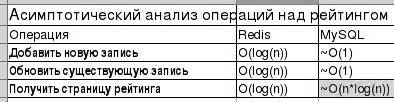
\includegraphics[width=10cm]{19_big_o_small.jpeg}

Как видим, серьёзной проблемой MySQL является очень дорогое получение страницы рейтинга.

Результат запуска бенчмарков отражен в сводной таблице:

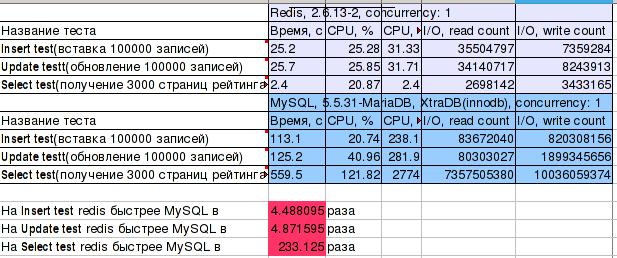
\includegraphics[width=10cm]{19_table_small.jpeg}

Как видно из таблицы, Redis значительно превосходит MySQL по производительности. На операциях вставки и обновления производительность выше почти в 5 раз, на операциях выборки превосходство просто подавляющее: 230 раз. При этом наличие необходимых индексов в MySQL таблице никак не влияет на производительность теста.

Несмотря на впечатляющие цифры на данном тесте, при анализе пригодности Redis к реализации других подзадач был выявлен ряд недостатков Redis: невозможность мультисортировки, избыточность данных при реализации рейтингов по уровню, проблемы с построением рейтинга среди друзей. Поэтому при решении задач построения различных игровых рейтингов оптимальным решением является использование этих двух СУБД в одной связке.

\end{document}
 
\documentclass[10pt, a5paper]{article}
\usepackage{pdfpages}
\usepackage{parallel}
\usepackage[T2A]{fontenc}
\usepackage{ucs}
\usepackage[utf8x]{inputenc}
\usepackage[polish,english,russian]{babel}
\usepackage{hyperref}
\usepackage{rotating}
\usepackage[inner=2cm,top=1.8cm,outer=2cm,bottom=2.3cm,nohead]{geometry}
\usepackage{listings}
\usepackage{graphicx}
\usepackage{wrapfig}
\usepackage{longtable}
\usepackage{indentfirst}
\usepackage{array}
\newcolumntype{P}[1]{>{\raggedright\arraybackslash}p{#1}}
\frenchspacing
\usepackage{fixltx2e} %text sub- and superscripts
\usepackage{icomma} % коскі ў матэматычным рэжыме
\PreloadUnicodePage{4}

\newcommand{\longpage}{\enlargethispage{\baselineskip}}
\newcommand{\shortpage}{\enlargethispage{-\baselineskip}}

\def\switchlang#1{\expandafter\csname switchlang#1\endcsname}
\def\switchlangbe{
\let\saverefname=\refname%
\def\refname{Літаратура}%
\def\figurename{Іл.}%
}
\def\switchlangen{
\let\saverefname=\refname%
\def\refname{References}%
\def\figurename{Fig.}%
}
\def\switchlangru{
\let\saverefname=\refname%
\let\savefigurename=\figurename%
\def\refname{Литература}%
\def\figurename{Рис.}%
}

\hyphenation{admi-ni-stra-tive}
\hyphenation{ex-pe-ri-ence}
\hyphenation{fle-xi-bi-li-ty}
\hyphenation{Py-thon}
\hyphenation{ma-the-ma-ti-cal}
\hyphenation{re-ported}
\hyphenation{imp-le-menta-tions}
\hyphenation{pro-vides}
\hyphenation{en-gi-neering}
\hyphenation{com-pa-ti-bi-li-ty}
\hyphenation{im-pos-sible}
\hyphenation{desk-top}
\hyphenation{elec-tro-nic}
\hyphenation{com-pa-ny}
\hyphenation{de-ve-lop-ment}
\hyphenation{de-ve-loping}
\hyphenation{de-ve-lop}
\hyphenation{da-ta-ba-se}
\hyphenation{plat-forms}
\hyphenation{or-ga-ni-za-tion}
\hyphenation{pro-gramming}
\hyphenation{in-stru-ments}
\hyphenation{Li-nux}
\hyphenation{sour-ce}
\hyphenation{en-vi-ron-ment}
\hyphenation{Te-le-pathy}
\hyphenation{Li-nux-ov-ka}
\hyphenation{Open-BSD}
\hyphenation{Free-BSD}
\hyphenation{men-ti-on-ed}
\hyphenation{app-li-ca-tion}

\def\progref!#1!{\texttt{#1}}
\renewcommand{\arraystretch}{2} %Іначай формулы ў матрыцы зліпаюцца з лініямі
\usepackage{array}

\def\interview #1 (#2), #3, #4, #5\par{

\section[#1, #3, #4]{#1 -- #3, #4}
\def\qname{LVEE}
\def\aname{#1}
\def\q ##1\par{{\noindent \bf \qname: ##1 }\par}
\def\a{{\noindent \bf \aname: } \def\qname{L}\def\aname{#2}}
}

\def\interview* #1 (#2), #3, #4, #5\par{

\section*{#1\\{\small\rm #3, #4. #5}}

\def\qname{LVEE}
\def\aname{#1}
\def\q ##1\par{{\noindent \bf \qname: ##1 }\par}
\def\a{{\noindent \bf \aname: } \def\qname{L}\def\aname{#2}}
}


\begin{document}

\title{<<Долгоиграющие>> базы данных PostgreSQL}%\footnote{Текст данных и последующих тезисов, кроме специально оговоренных случаев, доступен под лицензией Creative Commons Attribution"=ShareAlike 3.0}

\author{Владимир Рубанов\footnote{Москва, Россия; \url{vrub77@gmail.com}}}
\maketitle

\begin{abstract}
The talk presents a set of technologies and tools used at ROSA to develop its products, first of all Linux distributions. These tools are open source and can be used by other distribution developers to automate various tasks, such as checking repository consistency, ABI compatibility analysis, tracking of upstream components evolution, package difference analysis and, finally, the ABF integrated development and build system.
\end{abstract}

Разработка сложного многокомпонентного программного обеспечения, включающего сотни тысяч файлов с исходными кодами и тысячи модулей, требует специальных средств автоматизации.

Для автоматизации разработки продуктов компании ROSA применяется набор инструментов, которые являются свободными и могут быть использованы разработчиками других дистрибутивов для автоматизации следующих задач:

\begin{enumerate}
  \item Проверка замкнутости и непротиворечивости репозиториев.
  \item Тестирование обратной совместимости ABI/API дистрибутива.
  \item Отслеживание эволюции upstream компонентов и поддержка принятия решений по обновлению.
  \item Анализ отличий различных версий пакетов.
  \item Интегрированная система разработки и сборки ABF.
\end{enumerate}

Разработка сложногого многокомпонентного программного обеспечения, включающего сотни тысяч файлов с исходными кодами и тысячи модулей, требует специальных средств автоматизации.

Для автоматизации разработки продуктов компании ROSA применяется набор инструментов, которые являются свободными и могут быть использованы разработчиками других дистрибутивов для автоматизации следующих задач:

\begin{enumerate}
  \item Проверка замкнутости и непротиворечивости репозиториев.
  \item Тестирование обратной совместимости ABI/API дистрибутива.
  \item Отслеживание эволюции upstream компонентов и поддержка принятия решений по обновлению.
  \item Анализ отличий различных версий пакетов.
  \item Интегрированная система разработки и сборки ABF.
\end{enumerate}

\textbf{URPM Repoclosure} (реализация на Perl, распространяется под GPLv2) контролирует замкнутость репозитория по зависимостям и может использоваться как для статического, так и для динамического анализа собранного репозитория. Замкнутость репозитория является необходимым условием корректной установки пакетов. В статическом режиме анализа производится быстрая проверка атрибутов пакетов — предоставляемых (provides) и требуемых (requires и suggests) зависимостей, с целью выявления сломанных зависимостей, т.~е. требуемых пакетами, но не предоставляемых ни одним из них. В динамическом режиме происходит реальная установка всех пакетов и анализ ошибок менеджера пакетов. Регулярные запуски инструмента на стадии активной разработки репозитория позволяют избавиться от большинства проблем с установкой пакетов. Инструмент входит в состав пакета \textbf{URPM Tools}, в котором можно найти много других полезных инструментов для анализа репозитория, такие как \textbf{URPM Repograph} (Python, GPLv2) для визуализации графов зависимостей и поиска кольцевых зависимостей, \textbf{URPM Repodiff} (Python, GPLv2) для сравнения репозиториев и др.

\textbf{ABI Compliance Checker} (Perl, LGPLv2) ориентирован на разработчиков библиотек и мэйнтейнеров пакетов и позволяет проводить анализ обратной совместимости версий системных библиотек. Современные дистрибутивы Linux содержат тысячи библиотек, имеющие огромное число зависимостей между собой. Обновление любой из них может нарушить работу многих других и в итоге привести к некорректной работе пользовательских приложений. Инструмент позволяет выявить опасные изменения в API и ABI библиотеки и помочь мэйнтейнеру адаптировать компоненты дистрибутива к новой версии библиотеки или принять решение по изменению ее soname. Разработчики же библиотек могут использовать инструмент для выпуска обратно совместимых новых версий, чтобы у их пользователей не было проблем с обновлением. Инструмент анализирует либо заголовочные файлы библиотеки путем построения их синтаксического дерева разбора с помощью компилятора GCC, либо ее debug"=информацию с помощью дополнительного инструмента \textbf{ABI Dumper} (Perl, LGPLv2) и состав виртуальных таблиц с помощью инструмента \textbf{Vtable Dumper} (C, GPLv2).

Для мониторинга и анализа библиотек в апстриме применяется \textbf{Upstream Tracker}, что позволяет своевременно отслеживать новые версии и изменения в API/ABI. Инструмент представляет собой online ресурс, предоставляющий в публичный доступ отчеты инструмента ABI Compliance Checker об изменениях в API и ABI новых версий более чем 500 самых популярных библиотек в Linux. В первую очередь инструмент используется мэйнтейнерами для принятия решения об обновлении библиотеки или о выборе более подходящей версии библиотеки для конкретной версии дистрибутива. Также инструмент используется разработчиками библиотек и помогает им выпускать обратно совместимые версии, которые затем легче обновлять мэйнтейнерам дистрибутивов. Новые библиотеки добавляются незамедлительно и безвозмездно по запросу пользователей, заинтересованных в анализе этих библиотек.

Для поддержания актуальности дистрибутива важно иметь свежие, но при этом стабильные версии программ. Поэтому важно отслеживать не только апстрим, но и использование различных версий определенного пакета в других дистрибутивах, что косвенно служит показателем стабильности той или иной версии. Для этого необходимо уметь систематически сравнивать версии пакетов в своем дистрибутиве с версиями у коллег и определять устаревшие. Эта задача выполняется инструментом \textbf{Updates Tracker}.

Визуализация и классификация изменений в пакетах осуществляется с помощью инструмента \textbf{PkgDiff} (Perl, GPLv2). Основной задачей мэйнтейнеров в повседневной работе является обновление пакетов. Чтобы убедиться в безопасности обновления пакета для системы, мэйнтейнеру необходимо просмотреть изменения в определенных файлах пакета. Инструмент разделяет файлы по группам, так чтобы мэйнтейнер мог выбрать нужную ему группу и просмотреть изменения в файлах этой группы с помощью удобного визуального отчета. Инструмент может сравнивать как бинарные пакеты RPM или Deb, так и архивы с исходными кодами. На основе этого инструмента построен также инструмент \textbf{DistDiff} (Perl, GPLv2) для комплексного сравнения различных версий дистрибутива посредством анализа всех его старых и новых пакетов.

Система разработки и сборки \textbf{ROSA ABF} представляет собой систему для хостинга и разработки дистрибутивов на основе Linux и приложений для них, предоставляет безопасную среду, позволяющую собирать пакеты под множество дистрибутивов. В числе возможностей следует уопмянуть встроенный трекер задач, контекстную WIKI, а также интеграцию с системой контроля версий Git. Система также включает функцию централизованной доставки обновлений для клиентских машин (как пользовательских, так и серверных) и может быть использована в качестве сервера непрерывной интеграции.


\end{document}





\documentclass[10pt, a5paper]{article}
\usepackage{pdfpages}
\usepackage{parallel}
\usepackage[T2A]{fontenc}
\usepackage{ucs}
\usepackage[utf8x]{inputenc}
\usepackage[polish,english,russian]{babel}
\usepackage{hyperref}
\usepackage{rotating}
\usepackage[inner=2cm,top=1.8cm,outer=2cm,bottom=2.3cm,nohead]{geometry}
\usepackage{listings}
\usepackage{graphicx}
\usepackage{wrapfig}
\usepackage{longtable}
\usepackage{indentfirst}
\usepackage{array}
\newcolumntype{P}[1]{>{\raggedright\arraybackslash}p{#1}}
\frenchspacing
\usepackage{fixltx2e} %text sub- and superscripts
\usepackage{icomma} % коскі ў матэматычным рэжыме
\PreloadUnicodePage{4}

\newcommand{\longpage}{\enlargethispage{\baselineskip}}
\newcommand{\shortpage}{\enlargethispage{-\baselineskip}}

\def\switchlang#1{\expandafter\csname switchlang#1\endcsname}
\def\switchlangbe{
\let\saverefname=\refname%
\def\refname{Літаратура}%
\def\figurename{Іл.}%
}
\def\switchlangen{
\let\saverefname=\refname%
\def\refname{References}%
\def\figurename{Fig.}%
}
\def\switchlangru{
\let\saverefname=\refname%
\let\savefigurename=\figurename%
\def\refname{Литература}%
\def\figurename{Рис.}%
}

\hyphenation{admi-ni-stra-tive}
\hyphenation{ex-pe-ri-ence}
\hyphenation{fle-xi-bi-li-ty}
\hyphenation{Py-thon}
\hyphenation{ma-the-ma-ti-cal}
\hyphenation{re-ported}
\hyphenation{imp-le-menta-tions}
\hyphenation{pro-vides}
\hyphenation{en-gi-neering}
\hyphenation{com-pa-ti-bi-li-ty}
\hyphenation{im-pos-sible}
\hyphenation{desk-top}
\hyphenation{elec-tro-nic}
\hyphenation{com-pa-ny}
\hyphenation{de-ve-lop-ment}
\hyphenation{de-ve-loping}
\hyphenation{de-ve-lop}
\hyphenation{da-ta-ba-se}
\hyphenation{plat-forms}
\hyphenation{or-ga-ni-za-tion}
\hyphenation{pro-gramming}
\hyphenation{in-stru-ments}
\hyphenation{Li-nux}
\hyphenation{sour-ce}
\hyphenation{en-vi-ron-ment}
\hyphenation{Te-le-pathy}
\hyphenation{Li-nux-ov-ka}
\hyphenation{Open-BSD}
\hyphenation{Free-BSD}
\hyphenation{men-ti-on-ed}
\hyphenation{app-li-ca-tion}

\def\progref!#1!{\texttt{#1}}
\renewcommand{\arraystretch}{2} %Іначай формулы ў матрыцы зліпаюцца з лініямі
\usepackage{array}

\def\interview #1 (#2), #3, #4, #5\par{

\section[#1, #3, #4]{#1 -- #3, #4}
\def\qname{LVEE}
\def\aname{#1}
\def\q ##1\par{{\noindent \bf \qname: ##1 }\par}
\def\a{{\noindent \bf \aname: } \def\qname{L}\def\aname{#2}}
}

\def\interview* #1 (#2), #3, #4, #5\par{

\section*{#1\\{\small\rm #3, #4. #5}}

\def\qname{LVEE}
\def\aname{#1}
\def\q ##1\par{{\noindent \bf \qname: ##1 }\par}
\def\a{{\noindent \bf \aname: } \def\qname{L}\def\aname{#2}}
}

\begin{document}
\title{Introspecting Web Applications with Haskell and Erlang}
\author{Vladimir Kirillov \footnote{Kyiv, Ukraine}}
\maketitle

\begin{abstract}
Web is about queues thus you should use platforms that have lightweight threads because they are easy to write and debug or you die in a trace hell.
\end{abstract}

In production environments knowing what's going on is important: most bugs happen in production which are hard to come up with in lab environments. Thus, the debugging is usually performed by operations team with production binary builds of software, which means that regular profiling and debugger accesses are limited.

The above implies that one must neither disrupt live services in order to obtain required information to fix the issue nor that it is easy to generate the same set of service requests to replicate the issue in a preproduction (whatever) environment due to resource limitations (money, etc).

This means that given the limited set of tools and techniques the engineer should quickly collect any possible state of the world and pass it for analysis.

Modern application workloads, namely concurrent queue processing and long-living connections enforce a specific set of constraints on the runtime environment that are transitively applied to the development environment (VM, app design, libraries, language).

Logging, which is a common practice of leaving bread crumbs through the system, doesn't always help because they usually tend to represent sequences of ongoing events at the specific point of time (aka immediate state) shadowing the waiting queue of events, events that are stuck in the middle of a processing pipeline, simply saying, the big picture (aka entity). As a bonus, logging is often scattered throughout the distributed system which brings challenges like restoring the correct sequence of events (out-of-sync clocks) and simply correctly gathering the log data which is actually relevant to the problem (solutions to this challenge are left out of scope of this article).

So the problem effectively comes down to a problem of having a software platform that lets you effectively observe its state at run time (obviously, the latter excludes the possibility of using a traditional stop-the-world debugger).

A common example of such a software platform is an operating system and its kernel. For example, a Linux kernel exposes multiple interfaces (namely {\tt proc(5)}, {\tt netlink(7)}, {\tt sysfs}) to inspect its internal data structures and sample its runtime (see \href{http://joyent.com/blog/linux-performance-analysis-and-tools-brendan-gregg-s-talk-at-scale-11x}{linuxperf} for more).

However it becomes tempting to the operations engineer to use the system-wide introspection tools instead of the application-specific because many of those are available thus imposing the \href{http://queue.acm.org/detail.cfm?id=2413037}{streetlight anti-method} of debugging.

This brings us to the necessity of an application operating systems that possesses control over the application resources and keeps track of internal processing queues effectively giving introspection abilities.

However rolling such a system on a programmer's own usually demonstrates suffering from \href{http://en.wikipedia.org/wiki/Not_invented_here}{NIH} syndrome. Moreover, this exhibits the effectiveness of \href{http://en.wikipedia.org/wiki/Greenspun's_tenth_rule}{Greenspun}'s tenth rule of programming (substitute any technology for your in the LHS of the statement):

\begin{quote}%
Any sufficiently complicated C or Fortran program contains an ad hoc, informally-specified, bug-ridden, slow implementation of half of Common Lisp.
\end{quote}
Or, applying the rule to modern web-like workloads with high concurrency we end up with \href{http://rvirding.blogspot.com/2008/01/virdings-first-rule-of-programming.html}{Virding}'{}s first rule of programming:

\begin{quote}%
Any sufficiently complicated concurrent program in another language contains an ad hoc informally-specified bug-ridden slow implementation of half of Erlang.

\end{quote}
In practice, it's best to rely on the features that are built-in to the runtime platform, such as Haskell's {\tt GHC RTS} and Erlang's {\tt beam}. Both platforms employ a programming model with lightweight (or green) threads, also commonly known as $ M:N $ model, where $ N < M $ due to the housekeeping cost of OS threads.

It's also worth noting that it's practically inefficient to implement $ M:N $ model in non-functional languages with shared mutable data and complexities of implementing blocking system calls as non-blocking (tracking of this problem can be started from \href{http://www.kegel.com/c10k.html#1:1}{c10kthreading}).

On the contrary, bytecode interpreters that are the default implementations of dynamic languages like Python, Ruby, PHP and runtimes like NodeJS and JVM are inconvenient due to employed programming model of asynchronous callbacks and thread pools that significantly harden debugging because a single processing pipeline is scattered across multiple threads of control with different operation semantics.

The conference talk (and slides) will cover practical aspects of the problem and will demonstrate possible solutions to it.

\documentclass[10pt, a5paper]{article}
\usepackage{pdfpages}
\usepackage{parallel}
\usepackage[T2A]{fontenc}
\usepackage{ucs}
\usepackage[utf8x]{inputenc}
\usepackage[polish,english,russian]{babel}
\usepackage{hyperref}
\usepackage{rotating}
\usepackage[inner=2cm,top=1.8cm,outer=2cm,bottom=2.3cm,nohead]{geometry}
\usepackage{listings}
\usepackage{graphicx}
\usepackage{wrapfig}
\usepackage{longtable}
\usepackage{indentfirst}
\usepackage{array}
\newcolumntype{P}[1]{>{\raggedright\arraybackslash}p{#1}}
\frenchspacing
\usepackage{fixltx2e} %text sub- and superscripts
\usepackage{icomma} % коскі ў матэматычным рэжыме
\PreloadUnicodePage{4}

\newcommand{\longpage}{\enlargethispage{\baselineskip}}
\newcommand{\shortpage}{\enlargethispage{-\baselineskip}}

\def\switchlang#1{\expandafter\csname switchlang#1\endcsname}
\def\switchlangbe{
\let\saverefname=\refname%
\def\refname{Літаратура}%
\def\figurename{Іл.}%
}
\def\switchlangen{
\let\saverefname=\refname%
\def\refname{References}%
\def\figurename{Fig.}%
}
\def\switchlangru{
\let\saverefname=\refname%
\let\savefigurename=\figurename%
\def\refname{Литература}%
\def\figurename{Рис.}%
}

\hyphenation{admi-ni-stra-tive}
\hyphenation{ex-pe-ri-ence}
\hyphenation{fle-xi-bi-li-ty}
\hyphenation{Py-thon}
\hyphenation{ma-the-ma-ti-cal}
\hyphenation{re-ported}
\hyphenation{imp-le-menta-tions}
\hyphenation{pro-vides}
\hyphenation{en-gi-neering}
\hyphenation{com-pa-ti-bi-li-ty}
\hyphenation{im-pos-sible}
\hyphenation{desk-top}
\hyphenation{elec-tro-nic}
\hyphenation{com-pa-ny}
\hyphenation{de-ve-lop-ment}
\hyphenation{de-ve-loping}
\hyphenation{de-ve-lop}
\hyphenation{da-ta-ba-se}
\hyphenation{plat-forms}
\hyphenation{or-ga-ni-za-tion}
\hyphenation{pro-gramming}
\hyphenation{in-stru-ments}
\hyphenation{Li-nux}
\hyphenation{sour-ce}
\hyphenation{en-vi-ron-ment}
\hyphenation{Te-le-pathy}
\hyphenation{Li-nux-ov-ka}
\hyphenation{Open-BSD}
\hyphenation{Free-BSD}
\hyphenation{men-ti-on-ed}
\hyphenation{app-li-ca-tion}

\def\progref!#1!{\texttt{#1}}
\renewcommand{\arraystretch}{2} %Іначай формулы ў матрыцы зліпаюцца з лініямі
\usepackage{array}

\def\interview #1 (#2), #3, #4, #5\par{

\section[#1, #3, #4]{#1 -- #3, #4}
\def\qname{LVEE}
\def\aname{#1}
\def\q ##1\par{{\noindent \bf \qname: ##1 }\par}
\def\a{{\noindent \bf \aname: } \def\qname{L}\def\aname{#2}}
}

\def\interview* #1 (#2), #3, #4, #5\par{

\section*{#1\\{\small\rm #3, #4. #5}}

\def\qname{LVEE}
\def\aname{#1}
\def\q ##1\par{{\noindent \bf \qname: ##1 }\par}
\def\a{{\noindent \bf \aname: } \def\qname{L}\def\aname{#2}}
}

\begin{document}
\title{Пиратское движение в Беларуси}
\author{Михаил Волчек \footnote{Минск, Беларусь}}
\maketitle
\begin{abstract}
This presentation opens belarusian pirates' agenda, describes what they do and ups some actual issues for free software community. Do we ready to comminucate and build bridges for overcoming common challenges?
\end{abstract}
Беларусь не является тихой гаванью и не может считаться полностью избавленной от проблем, которые имеют интернет-пользователи по всему миру: несбалансированное копирайт-законодательство, нелегальный сбор данных коммерческими и правительственными структурами и т.д.

В 2013 году в Беларуси появился Пиратский Центр, имеющий веб-сайт по адресу pirates.by и ориентированный на то, чтобы активно заниматься проблемами беларусских интернет-пользователей (в т.ч. через просветительскую деятельность).
Пиратский центр является полноправным членом Pirate Party International (PPI) -- международной организации, действующей с 2009 года и ставящей своей целью способствовать взаимодействию появляющихся пиратских партий, групп и движений по всему миру.

Пиратские партии концентрируются на цифровых правах, но не только. В этот список входят реформа копирайта (патентной системы), анонимность и приватность в сети, доступный интернет (как право), нейтралитет сети, вовлеченность людей в принятие решений, прозрачность управления в обществе, экономика, ориентированная на человека, а не рост цифр ВВП.

Согласно анонсам на pirates.by, центр на текущий момент занимается:

\begin{enumerate}
  \item Продвижением среди пользователей интернета криптографических
инструментов как средств для приватного и анонимного интернета. Форма популяризации -- криптовечеринки.
  \item Раскрытием темы свободных лицензий как одной из альтернатив копирайту. Форма популяризации -- открытые лекции с различными творческими сообществами и людьми, аудиоконференции, образовательный клуб, просмотры фильмов о сетевых сообществах.
  \item Изучением инструментов, реализованных на открытых платформах для
выработки и принятия решений в больших группах (например,
Liquidfeedback, adhocracy, wikiarguments).
\end{enumerate}

Перечисленный набор активностей направлен на популяризацию знаний о цифровых правах человека, расширение кругозора и повышение уровня сетевой и компьютерной грамотности пользователей.

Следует учитывать, что под цифровыми правами в данном случае понимаются права, описанные во Всеобщей Декларации Прав Человека, применённые в цифровых технологиях (осн. Сеть), а под копирайтом понимается набор законов и международных договоров, регулирующих культуру, медиа, науку и другие сферы общества, связанные с производством, потреблением и распределением продуктов индустрии контента (фильмы, музыка, программы, игры, книги и т.д).

\end{document}

%\chapter{LVEE Winter 2012}
\documentclass[10pt, a5paper]{article}
\usepackage{pdfpages}
\usepackage{parallel}
\usepackage[T2A]{fontenc}
\usepackage{ucs}
\usepackage[utf8x]{inputenc}
\usepackage[polish,english,russian]{babel}
\usepackage{hyperref}
\usepackage{rotating}
\usepackage[inner=2cm,top=1.8cm,outer=2cm,bottom=2.3cm,nohead]{geometry}
\usepackage{listings}
\usepackage{graphicx}
\usepackage{wrapfig}
\usepackage{longtable}
\usepackage{indentfirst}
\usepackage{array}
\newcolumntype{P}[1]{>{\raggedright\arraybackslash}p{#1}}
\frenchspacing
\usepackage{fixltx2e} %text sub- and superscripts
\usepackage{icomma} % коскі ў матэматычным рэжыме
\PreloadUnicodePage{4}

\newcommand{\longpage}{\enlargethispage{\baselineskip}}
\newcommand{\shortpage}{\enlargethispage{-\baselineskip}}

\def\switchlang#1{\expandafter\csname switchlang#1\endcsname}
\def\switchlangbe{
\let\saverefname=\refname%
\def\refname{Літаратура}%
\def\figurename{Іл.}%
}
\def\switchlangen{
\let\saverefname=\refname%
\def\refname{References}%
\def\figurename{Fig.}%
}
\def\switchlangru{
\let\saverefname=\refname%
\let\savefigurename=\figurename%
\def\refname{Литература}%
\def\figurename{Рис.}%
}

\hyphenation{admi-ni-stra-tive}
\hyphenation{ex-pe-ri-ence}
\hyphenation{fle-xi-bi-li-ty}
\hyphenation{Py-thon}
\hyphenation{ma-the-ma-ti-cal}
\hyphenation{re-ported}
\hyphenation{imp-le-menta-tions}
\hyphenation{pro-vides}
\hyphenation{en-gi-neering}
\hyphenation{com-pa-ti-bi-li-ty}
\hyphenation{im-pos-sible}
\hyphenation{desk-top}
\hyphenation{elec-tro-nic}
\hyphenation{com-pa-ny}
\hyphenation{de-ve-lop-ment}
\hyphenation{de-ve-loping}
\hyphenation{de-ve-lop}
\hyphenation{da-ta-ba-se}
\hyphenation{plat-forms}
\hyphenation{or-ga-ni-za-tion}
\hyphenation{pro-gramming}
\hyphenation{in-stru-ments}
\hyphenation{Li-nux}
\hyphenation{sour-ce}
\hyphenation{en-vi-ron-ment}
\hyphenation{Te-le-pathy}
\hyphenation{Li-nux-ov-ka}
\hyphenation{Open-BSD}
\hyphenation{Free-BSD}
\hyphenation{men-ti-on-ed}
\hyphenation{app-li-ca-tion}

\def\progref!#1!{\texttt{#1}}
\renewcommand{\arraystretch}{2} %Іначай формулы ў матрыцы зліпаюцца з лініямі
\usepackage{array}

\def\interview #1 (#2), #3, #4, #5\par{

\section[#1, #3, #4]{#1 -- #3, #4}
\def\qname{LVEE}
\def\aname{#1}
\def\q ##1\par{{\noindent \bf \qname: ##1 }\par}
\def\a{{\noindent \bf \aname: } \def\qname{L}\def\aname{#2}}
}

\def\interview* #1 (#2), #3, #4, #5\par{

\section*{#1\\{\small\rm #3, #4. #5}}

\def\qname{LVEE}
\def\aname{#1}
\def\q ##1\par{{\noindent \bf \qname: ##1 }\par}
\def\a{{\noindent \bf \aname: } \def\qname{L}\def\aname{#2}}
}


\begin{document}

\title{Telepathy-skykit}%\footnote{Текст данных и последующих тезисов, кроме специально оговоренных случаев, доступен под лицензией Creative Commons Attribution-ShareAlike 3.0}

\author{Максим Мельников\footnote{Минск, Беларусь; \url{}}}
\maketitle

\begin{abstract}
Telepathy-skykit, a Telepathy connection manager developed by the author, is presented. It implements Skype protocol support, and is based on Skype SDK for embedded development, known as SkypeKit. The project's goal is to use Skype without a `regular' desktop client, while using all features Telepathy provides: unified UI for all protocols, proper logging subsystem and Telepathy integration with Desktop Environment.
\end{abstract}

\subsection*{Telepathy}

Telepathy — программный каркас, используемый для создания программного обеспечения мгновенного обмена сообщениями, IP-телефонии или видеоконференций. Telepathy позволяет создавать приложения c помощью компонентов через систему межпроцессного взаимодействия D-Bus. При этом, logger, connection manager и UI работают в отдельных процессах.

\begin{figure}[t]
  \centering
  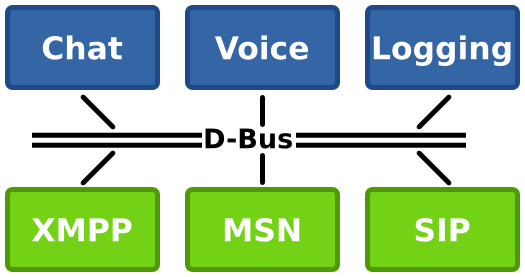
\includegraphics[width=6cm]{101_2013_w_Melnikau_tao}
\end{figure}

Для telepathy уже разработана поддержка основных протоколов:
\begin{itemize}
\item Gabble "--- Jabber/XMPP, включая Jingle;
\item Rakia "--- SIP;
\item Haze "--- обёртка над libpurple, внутренней библиотекой Pidgin; поддерживает все протоколы, с которыми умеет работать сам Pidgin.
\end{itemize}

С точки зрения UI, основными приложениями являются следующие два:
\begin{itemize}
\item Empathy, обладающий хорошей интеграция с Gnome и Evalution Data Server;
\item KDE-Telepathy, предоставляющий аналогичную интеграцию с KDE.
\end{itemize}

Оба приложения поддерживают передачу звука и видео; также есть и другие, менее функциональные.

Также, уже разработаны следующие компоненты:
\begin{itemize}
\item logger "--- сервис отвечающий за хранение и предоставление логов по запросу
\item mission-control "--- управление аккаунтами
\end{itemize}

Таким образом, Telepathy "--- хорошо проработанный, модульный framework, содержащий много готовых унифицированных компонентов, и позволяющий которые легко добавлять новые или расширять существующие.

\subsection*{SkypeKit}
SkypeKit "--- коллекция утилит и API, которые позволяют разработать собственное устройство/приложение с поддержкой skype протокола: чат, аудио и видео. Причём разработан он с возможностью использования на большом количестве различных чипов, операционных систем и устройств, и является «безинтерфейсным».
\begin{figure}[b]
  \centering
  
\includegraphics[width=8cm]{101_2013_w_Melnikau_skypekit}
\end{figure}
Под Linux поддерживаются следующие аппаратные архитектуры: armv5le,
armv6le, armv7le, x86. Разработка может вестись на C++, C\#, java, python. При этом сам SkypeKit-демон не содержит UI, и для интеграции с системой может использовать ALSA, X11 OpenGL, либо GStreamer.

\subsection*{Skype в Telepathy}

Поддержка Skype в Telepathy до этого существовала в единственном виде: skype4pidgin "--- plugin для Pidgin (libpurle), поддерживающий Skype, который подключается как один из libpurple"=протоколов, через telepathy"=haze. Однако у неё существуют большие ограничения: отсутствие поддержки аудио и видео, а также части функциональности чата, vCard и других не базовых возможностей.

Альтернативный вариант, разработанный автором: telepathy"=sky\-kit "--- connection manager, реализующий поддержку Skype для Telepathy. При этом используется embedded-демон SkypeKit, который реализует поддержку протокола Skype, а telepathy"=skypekit при этом представляет собой лишь wrapper.

Для простоты реализации (прототипирования) был выбран Python. А для интеграции с Telepathy используется библиотека telepathy"=python, в которую была добавлена поддержка необходимого функциональности.

В данный момент реализованы:
\begin{itemize}
\item чат "--- самая базовая функциональность, общение один на один;
\item контакт-лист;
\item поддержка аватарок и карточка профиля (vCard).
\end{itemize}

Планы на будущее:
\begin{itemize}
\item конференции "--- очень часто используемая функциональность;
\item интеграция с OS "--- автоматический запуск демона при DBus-запросе и т.~д.;
\item аудио/видео звонки "--- хотя бы на уровне «proof of concept».
\end{itemize}
\begin{figure}[h]
  \centering
  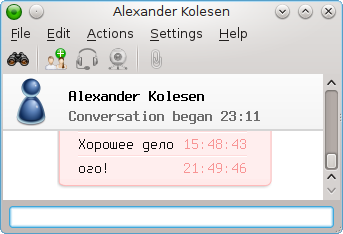
\includegraphics[width=6cm]{101_2013_w_Melnikau_ktpskype}
\end{figure}

\let\saverefname=\refname%
\def\refname{Полезные ссылки}%
\begin{thebibliography}{9}
\bibitem{meln1} \url{http://telepathy.freedesktop.org/wiki/}
\bibitem{meln2} \url{https://developer.skype.com/public/skypekit/}
\bibitem{meln3} \url{https://github.com/max-posedon/telepathy-skykit}
\bibitem{meln4} \url{https://github.com/max-posedon/telepathy-python}
\end{thebibliography}
\let\refname=\saverefname%

\end{document}





\documentclass[10pt, a5paper]{article}
\usepackage{pdfpages}
\usepackage{parallel}
\usepackage[T2A]{fontenc}
\usepackage{ucs}
\usepackage[utf8x]{inputenc}
\usepackage[polish,english,russian]{babel}
\usepackage{hyperref}
\usepackage{rotating}
\usepackage[inner=2cm,top=1.8cm,outer=2cm,bottom=2.3cm,nohead]{geometry}
\usepackage{listings}
\usepackage{graphicx}
\usepackage{wrapfig}
\usepackage{longtable}
\usepackage{indentfirst}
\usepackage{array}
\newcolumntype{P}[1]{>{\raggedright\arraybackslash}p{#1}}
\frenchspacing
\usepackage{fixltx2e} %text sub- and superscripts
\usepackage{icomma} % коскі ў матэматычным рэжыме
\PreloadUnicodePage{4}

\newcommand{\longpage}{\enlargethispage{\baselineskip}}
\newcommand{\shortpage}{\enlargethispage{-\baselineskip}}

\def\switchlang#1{\expandafter\csname switchlang#1\endcsname}
\def\switchlangbe{
\let\saverefname=\refname%
\def\refname{Літаратура}%
\def\figurename{Іл.}%
}
\def\switchlangen{
\let\saverefname=\refname%
\def\refname{References}%
\def\figurename{Fig.}%
}
\def\switchlangru{
\let\saverefname=\refname%
\let\savefigurename=\figurename%
\def\refname{Литература}%
\def\figurename{Рис.}%
}

\hyphenation{admi-ni-stra-tive}
\hyphenation{ex-pe-ri-ence}
\hyphenation{fle-xi-bi-li-ty}
\hyphenation{Py-thon}
\hyphenation{ma-the-ma-ti-cal}
\hyphenation{re-ported}
\hyphenation{imp-le-menta-tions}
\hyphenation{pro-vides}
\hyphenation{en-gi-neering}
\hyphenation{com-pa-ti-bi-li-ty}
\hyphenation{im-pos-sible}
\hyphenation{desk-top}
\hyphenation{elec-tro-nic}
\hyphenation{com-pa-ny}
\hyphenation{de-ve-lop-ment}
\hyphenation{de-ve-loping}
\hyphenation{de-ve-lop}
\hyphenation{da-ta-ba-se}
\hyphenation{plat-forms}
\hyphenation{or-ga-ni-za-tion}
\hyphenation{pro-gramming}
\hyphenation{in-stru-ments}
\hyphenation{Li-nux}
\hyphenation{sour-ce}
\hyphenation{en-vi-ron-ment}
\hyphenation{Te-le-pathy}
\hyphenation{Li-nux-ov-ka}
\hyphenation{Open-BSD}
\hyphenation{Free-BSD}
\hyphenation{men-ti-on-ed}
\hyphenation{app-li-ca-tion}

\def\progref!#1!{\texttt{#1}}
\renewcommand{\arraystretch}{2} %Іначай формулы ў матрыцы зліпаюцца з лініямі
\usepackage{array}

\def\interview #1 (#2), #3, #4, #5\par{

\section[#1, #3, #4]{#1 -- #3, #4}
\def\qname{LVEE}
\def\aname{#1}
\def\q ##1\par{{\noindent \bf \qname: ##1 }\par}
\def\a{{\noindent \bf \aname: } \def\qname{L}\def\aname{#2}}
}

\def\interview* #1 (#2), #3, #4, #5\par{

\section*{#1\\{\small\rm #3, #4. #5}}

\def\qname{LVEE}
\def\aname{#1}
\def\q ##1\par{{\noindent \bf \qname: ##1 }\par}
\def\a{{\noindent \bf \aname: } \def\qname{L}\def\aname{#2}}
}


\def\vv!#1!{\texttt{#1}}
\begin{document}

\switchlang{be}

\title{Лінуксоўка ў новым фармаце, занатоўкі выпадковага ўдзельніка аргкамітэта}%\footnote{Текст данных и последующих тезисов, кроме специально оговоренных случаев, доступен под лицензией Creative Commons Attribution-ShareAlike 3.0}

\author{Андрэй Захарэвіч\footnote{Мінск, Беларусь; \url{andrej@zahar.ws}}}
\maketitle

\begin{abstract}
Minsk LUG monthly meetings. Explaining of new meeting format, giving a to do list of organizational Board and discussing organizational aims which was (or was not) reached.
\end{abstract}

\subsubsection*{Крыху пра гісторыю лінуксовак MLUG}

Безумоўна, лінуксоўкі ў Мінску — з'ява не новая. Яны налічваюць мінімум тры «пакаленні» ўдзельнікаў і мінімум адну спробу афіцыйна аформіць юрыдычную асобу, ад імя якой маглі б праводзіцца афіцыйныя камунікацыі MLUG, калі гэта спатрэбіцца.

Гэта цалкам натуральна, таму што Linux і іншыя Unix-падобныя сістэмы з'явіліся ў Мінску некалькі дзесяцігоддзяў таму, яшчэ ў мінулым стагоддзі і, вядома ж, карыстальнікі і аматары гэтых сістэм мелі патрэбу ў камунікацыі з аднадумцамі не толькі з выкарыстаннем нейкіх сеткавых тэхналогій, але і пры асабістай сустрэчы.

Я не даследваў пытанне глыбока, але першыя тэмы ў раздзеле «Линуксовка» на forum.linux.by датуюцца пачаткам 2002 года. Апошняя версія кіраўніцтва (HOWTO) па правядзенню лінуксовак на Wiki-старонцы \url{http://wiki.linux.by/wiki/Linuxovka\_HOWTO} была створаная 10 ліпеня 2007 года карыстальнікам Mend0za.

\subsubsection*{Інфармацыйныя рэсусы, якія аб'ядноўвалі Linux"=супольнасць на пачатку XXI стагоддзя}

Карыстаючыся толькі прыгаданым вышэй HOWTO, можна зазначыць, што існавалі як мінімум:

\begin{enumerate}
  \item Форум \url{forum.linux.by}. Месца, адносна жывое і зараз, калі значная частка актыўнасці, асабліва ў моладзі (да 25 год) перайшла ў сацыяльныя сеткі. Даволі даўно існуе больш для пачынаючых.
  \item Паштовыя рассылкі. Крыніца прыгадвае наступныя: \textit{«Весьма живая рассылка LVEE. На рассылки mlug-talks@ и mlug-announce@ подписано около 100 человек Подробности про рассылки. Наиболее серьёзная и многочисленная часть из подписчиков форумом пренебрегает, заслуженно считая его песочницей для пионеров.»}
  \item IRC: Каналы \vv!\#unix! і \vv!\#linux! на \vv!irc.bynets.org! і \vv!irc.by!.
  \item Fidonet: Эха \vv!bel.softw.unix!
\end{enumerate}

Такім чынам, магчымасці абвесціць лінуксоідам пра мерапрыемства на пачатку стагоддзя існавалі. І, як мне здаецца, казаць што ў спадзе лінуксовак вінаватая адсутнасць пляцовак для анонсаў і камунікацыі нельга.

\subsubsection*{Спад актыўнасці лінуксовак}

Наколькі ведаю, памяньшэнне актыўнасці лінуксовак гэта з'ява не спецыфічная для Беларусі, такое адбываецца ва ўсім свеце.

На маю думку, гэтак адбываецца таму, што лінуксоўкі ў тым выглядзе, як яны існавалі на той час, маглі прапанаваць усё менш і менш перавагаў у параўнанні з анлайн-камунікацыямі:
\begin{itemize}
  \item З гадамі ўсё больш дасканалая праца пашуковых сістэм дала магчымасць шукаць рэсурсы з адказамі на пытанні мінімальна разумеючы што ты шукаеш без асаблівых навыкаў складання пашуковых запытаў. А пашырэнне папулярнасці Linux дае магчымасць адшукаць адказы на большасць пытанняў, бо нехта ўжо імі цікавіўся.
  \item Пашырэнне выкарыстання камунікацый з дапамогай сацыяльных сетак прыводзіць да таго, што для сустрэчы ў афлайне павінна быць досыць важкая нагода. Проста адшукаць патрэбнага чалавека і абмеркаваць адно нейкае асобнае пытанне збольшага можна ўжо не толькі не ўставаючы з-за кампутара, але нават не ўключаючы яго, з дапамогай смартфона ці планшэта.
\end{itemize}

Безумоўна, адна нейкая праблема не магла пахаваць мерапрыемства, таму я бы яшчэ прыгадаў:
\begin{itemize}
  \item Нерэгулярнасць і непрадказальнасць раскладу. Арганізацыя лінуксовак, не кажучы пра змястоўны ўдзел у іх — гэта праца, якая патрабуе выдаткаваць сілы і час. Не маючы нейкага сур'ёзнага выніка гэтай працы ніхто не захоча займацца гэтым рэгулярна колькі-небуць працягчы час
  \item Фармат лінуксовак не даваў магчымасці расці далей
\end{itemize}

\subsubsection*{Класічны фармат лінуксовак у Мінску}

Безумоўна, не ўсе лінуксоўкі праходзілі так. Часам бывалі нейкія мерапрыемствы з дакладамі ў прыстасаваным для гэтага памяшканні, але большасць праходзіла ў нейкіх грамадскіх месцах, кшталту сквера на плошчы Якуба Коласа, ці на Бульвары Мулявіна.

З пэўнага часу часцей за ўсё выкарыстоўвалася пляцоўка збору «каля фантана», удзельнікі лінуксоўкі сустракаліся каля фантана «Вянок» (1972 год, скульптары А. Анікейчык, Л. Гумілеўскі, А. Заспіцкі) ў парку імя Я. Купалы. Як самае вядомае месца правядзення, «каля фантана» дало назву фармату лінуксовак.

\subsubsection*{Чаму б не адкапаць яшчэ раз «сустрэчы каля фантана»}

З'яўленне новага фармату лінуксовак было выкліканае тым, што класічны фармат «сустрэч з півам каля фантану» не задавальняў найбольш актыўных удзельнікаў з-за яго натуральных абмежаванняў:
\begin{enumerate}
  \item Неканструктыўнасць фармату не дазваляла праводзіць маштабных абмеркаванняў тэхнічных пытанняў і праблем. Цяжка расказваць пра нешта сур'ёзнае групе чалавек ў 10—15 пасярод парка ў цэнтры горада. Апроч таго, што нязручна паказваць нейкія схемы ці скрыншоты, дадаецца яшчэ той факт, што для такой сустрэчы паводле заканадаўства з мінулага года патрэбны дазвол гарадскіх ўлад з доўгім узгадненнем.
  \item Далёка не ўсім падабаўся сам фармат размовы «пад піва». Раней ці пазней лінуксоўка распадаецца на групы і драбіцца. Цытуючы прыгаданы вышэй HOWTO па лінуксоўках, \textit{«Да простят меня начинающие — но им обычно около-линуксовых тем хватает на полчаса-час (чтобы исчерпать круг интересов и личный опыт), потом начинается про бухло, тёлок и за жизнь.»}
  \item Сутракацца пад аткрытым небам зручна толькі пакуль пагода камфортная. То бок паводле самых аптымістычных ацэнак — 3—5 месяцаў на год.
\end{enumerate}

Апошні момант спрабавалі вырашаць, арганізуючы лінуксоўкі, напрыклад, у кафэ (\cite{zack1}). Аднак две першыя праблемы гэта не вырашала. Плюс, паколькі кафэ ў Мінску не хапае, то рэстаратары пачынаюць патрабаваць заказ не менш як на пэўную суму, папярэдні заказ. Магчымасць падсілкавацца пад час мерапрыемства можа быць не лішняй, але мы ж не для таго збіраліся?

Існуе меркаванне, што адной з прычын спаду (ці, нават, галоўнай прычынай ў некаторых інтэрпрэтацыях) было тое, што большасць удзельнікаў пасталелі і былі вельмі занятыя. Незгодны і лічу, што гэта звычайная адгаворка. Пры ўмове папярэдняга анонса даты мерапрыемства мінімум за 3—4 тыдні нават вельмі занятыя асобы знаходзяць час і сілы актыўна паўдзельнічаць. Некалькі прыкладаў (у выпадковым парадку):

\begin{itemize}
  \item {Максім Мельнікаў}, спецыяліст з кампаніі Wargaming, шчаслівы бацька (што не дадае вольнага часу і сіл) рэгулярна робіць цікавыя і змястоўныя даклады
  \item {Аляксей Чэвусаў}, таксама спецыяліст, бацька, FOSS актывіст і распрацоўшчык, што не зашкодзіла яму прыняць удзел у большасці лінуксовак, практычна кожны раз з дакладам, актыўна удзельнічаць у абмеркаваннях чужых дакладаў.
  \item {Уладзімір Шахаў}, зноўку ж, IT-спецыяліст, бацька, трэнер, галоўны сакратар аднаго з самых буйных спаборніцтваў па каратэ версіі WKF не толькі ў краіне, але і ў рэгіёне. Удзельнічае ў падрыхтоўцы лінуксовак ад з'яўлення іх у новым фармаце, рэгулярна робіць даклады, актыўна ўдзельнічае ў абмеркаваннях.
\end{itemize}

\subsubsection*{Што рабіць каб пераадолець спад актыўнасці}

Можа гэта не агульны рэцэпт, але падобна, што наш вопыт не ўнікальны і можа быць выкарыстаны іншымі.

Узяўшы за аснову фармат LVEE, арганізатары паспрабавалі стварыць нешта кшталту «міні-LVEE», які дазваляў бы і выказацца па нейкіх глабальных праблемах, і, пры неабходнасці, камерна абмеркаваць нешта ў кулуарах.

Стварэнне менавіта асобнага мерапрыемства было неабходнае таму, што LVEE праводзіцца раз на год, і далёка не усё будзе сэнс абмяркоўваць праз паўгады і больш. Павінна быць месца, куды не трэба выязджаць, каб задаць пытанні ці абмеркаваць нешта, куды могуць прыехаць і падзяліцца досведам людзі, якія не часта бываюць у Мінску. Снежаньская лінуксоўка традыцыйна з'яўляецца «эмігранцкай», у ёй удзельнічаюць спецыялісты з Мінску і Беларусі, якія зараз не жывуць на радзіме.

\subsubsection*{Што трэба, каб арганізаваць лінуксоўку}

\begin{enumerate}
  \item Патрэбнае памяшканне, якое зможа змясціць усіх ахвотных. У нашым выпадку павінна хапаць месца, каб рассадзіць 2—3 тузіны чалавек, плюс крыху вольнай прасторы, каб можна было рухацца і абмяркоўваць у купках.
  \item Патрэбныя актыўныя удзельнікі якія змогуць і захочуць патраціць час на падрыхтоўку цікавых і змястоўных дакладаў, адпавядаючых тэматыцы мерапрыемства.
  \item Патрэбныя актыўныя удзельнікі, хто зможа і захоча ўдзельнічаць у абмеркаваннях і задаваць пытанні (ці даваць парады) дакладчыкам.
  \item Патрэбнае размяшчэнне інфармацыі пра лінуксоўку на тэматычных пляцоўках (гл. раздзел «Дзе трэба размясціць інфармацыю пра лінуксоўку»).
  \item Месца правядзення павінна быць спланавана такім чынам, каб анонс мог быць змешчаны прыблізна за месяц. Большасць актыўных удзельнікаў мінімум прафесіяналы, шмат сярод іх і бацькоў, якім трэба папярэдне планаваць вольны час.
\end{enumerate}

\subsubsection*{Дзе трэба размясціць інфармацыю пра лінуксоўку}

Усе больш-менш звязаныя з тэматыкай пляцоўкі павінны быць накрытыя. На дадзены момант у мяне склаўся такі спіс пляцовак, на якія варта змясціць навіну пра лінуксоўку MLUG:

\begin{enumerate}
  \item Сайт MLUG. Ствараецца навіна з анонсам. (\cite{mlug}).
  \item Група MLUG на Google+. Эфектыўней за ўсё стварыць падзею у межах групы. (\cite{mlug-gplus}).
  \item Форум на Linux.by. Стварыць новую тэму ў раздзеле пра лінуксоўкі (\cite{mlug-forum}).
  \item Ліст з анонсам у групу рассылкі \vv!mlug-talks@! (\cite{mlug-talks}).
  \item Анонс падзеі на \url{meetup.by}
  \item Падзея ў Facebook, у групе MLUG (\cite{mlug-fb}).
  \item Падзея з анонсам у  Вконтакте MLUG (\cite{mlug-vk-1}) і Linux.by (\cite{mlug-vk-2}).
  \item Скінуць спасылку на анонс у Twitter (хэштэгі \vv!\#mlug! і \vv!\#linux!).
  \item Анонс у ЖЖ, можна ў тэматычных групах.
  \item Ліст з анонсам у LVEE mailing list.
\end{enumerate}

\subsubsection*{Што не атрымалася}

Не атрымалася пляцоўка для абмеркаванняў і навучання пачынаючых. Паколькі арганізатары не фільтруюць тэмы паводле ўзроўню аўдыторыі, а толькі паводле тэматыкі, каб пляцоўка давала магчымасці для пачынаючых яны іх павінны браць. То бок, агульная тэма і накірунак лінуксоўкі вызначаецца самімі ўдзельнікамі. Калі нехта прыйшоў пасядзець моўчкі ў куточку — пасядзіць, але тады на развіццё падзей ён не ўплывае наогул аніяк. Як прымусіць чалавека быць актыўным? Калі нехта параіць, буду ўдзячны.

\subsubsection*{Ці самотныя мы на гэтым свеце?}

Нашчасце, не! Друпал-клуб (falanster.by) праводзіць свае лінуксоўкі і іншыя мерапрыемствы.
Плюсы:

\begin{itemize}
  \item мерапрыемствы праводзяцца на ўзроўні зручным для тых, хто пачынае свой шлях у Лінукс;
  \item лінуксоўка вельмі камерная, менш за 10 чалавек, таму можа быць не так цяжка наважыцца задаць, абмеркаваць пытанні;
  \item большасць удзельнікаў лінуксоўкі рыхтуецца з нейкімі тэмамі, па выніках дакладаў па тэме праходзіць абмеркаванне.
\end{itemize}

І гэта не кажучы пра LVEE, якога з мінулага года стала ў два разы больш штогод.

\subsubsection*{Што рабіць далей?}

Кожны можа прыняць удзел у бліжэйшай рэгіянальнай лінуксоўцы ці стварыць сваю. 

\let\saverefname=\refname%
\def\refname{Спасылкі}%
\begin{thebibliography}{9}
\bibitem{zack1} \url{https://forum.linux.by/viewtopic.php?f=7\&t=9951}
\bibitem{mlug} \url{http://mlug.linux.by/}
\bibitem{mlug-gplus} \url{https://plus.google.com/communities/110681015343287679167}
\bibitem{mlug-forum} \url{https://forum.linux.by/viewforum.php?f=7}
\bibitem{mlug-talks} \url{http://groups.google.com/group/mlug-talks}
\bibitem{mlug-fb} \url{http://www.facebook.com/groups/46184759521/}
\bibitem{mlug-vk-1} \url{http://vk.com/club1271407}
\bibitem{mlug-vk-2} \url{http://vk.com/club8911620}
\end{thebibliography}
\let\refname=\saverefname%

\end{document}





\documentclass[10pt, a5paper]{article}
\usepackage{pdfpages}
\usepackage{parallel}
\usepackage[T2A]{fontenc}
\usepackage{ucs}
\usepackage[utf8x]{inputenc}
\usepackage[polish,english,russian]{babel}
\usepackage{hyperref}
\usepackage{rotating}
\usepackage[inner=2cm,top=1.8cm,outer=2cm,bottom=2.3cm,nohead]{geometry}
\usepackage{listings}
\usepackage{graphicx}
\usepackage{wrapfig}
\usepackage{longtable}
\usepackage{indentfirst}
\usepackage{array}
\newcolumntype{P}[1]{>{\raggedright\arraybackslash}p{#1}}
\frenchspacing
\usepackage{fixltx2e} %text sub- and superscripts
\usepackage{icomma} % коскі ў матэматычным рэжыме
\PreloadUnicodePage{4}

\newcommand{\longpage}{\enlargethispage{\baselineskip}}
\newcommand{\shortpage}{\enlargethispage{-\baselineskip}}

\def\switchlang#1{\expandafter\csname switchlang#1\endcsname}
\def\switchlangbe{
\let\saverefname=\refname%
\def\refname{Літаратура}%
\def\figurename{Іл.}%
}
\def\switchlangen{
\let\saverefname=\refname%
\def\refname{References}%
\def\figurename{Fig.}%
}
\def\switchlangru{
\let\saverefname=\refname%
\let\savefigurename=\figurename%
\def\refname{Литература}%
\def\figurename{Рис.}%
}

\hyphenation{admi-ni-stra-tive}
\hyphenation{ex-pe-ri-ence}
\hyphenation{fle-xi-bi-li-ty}
\hyphenation{Py-thon}
\hyphenation{ma-the-ma-ti-cal}
\hyphenation{re-ported}
\hyphenation{imp-le-menta-tions}
\hyphenation{pro-vides}
\hyphenation{en-gi-neering}
\hyphenation{com-pa-ti-bi-li-ty}
\hyphenation{im-pos-sible}
\hyphenation{desk-top}
\hyphenation{elec-tro-nic}
\hyphenation{com-pa-ny}
\hyphenation{de-ve-lop-ment}
\hyphenation{de-ve-loping}
\hyphenation{de-ve-lop}
\hyphenation{da-ta-ba-se}
\hyphenation{plat-forms}
\hyphenation{or-ga-ni-za-tion}
\hyphenation{pro-gramming}
\hyphenation{in-stru-ments}
\hyphenation{Li-nux}
\hyphenation{sour-ce}
\hyphenation{en-vi-ron-ment}
\hyphenation{Te-le-pathy}
\hyphenation{Li-nux-ov-ka}
\hyphenation{Open-BSD}
\hyphenation{Free-BSD}
\hyphenation{men-ti-on-ed}
\hyphenation{app-li-ca-tion}

\def\progref!#1!{\texttt{#1}}
\renewcommand{\arraystretch}{2} %Іначай формулы ў матрыцы зліпаюцца з лініямі
\usepackage{array}

\def\interview #1 (#2), #3, #4, #5\par{

\section[#1, #3, #4]{#1 -- #3, #4}
\def\qname{LVEE}
\def\aname{#1}
\def\q ##1\par{{\noindent \bf \qname: ##1 }\par}
\def\a{{\noindent \bf \aname: } \def\qname{L}\def\aname{#2}}
}

\def\interview* #1 (#2), #3, #4, #5\par{

\section*{#1\\{\small\rm #3, #4. #5}}

\def\qname{LVEE}
\def\aname{#1}
\def\q ##1\par{{\noindent \bf \qname: ##1 }\par}
\def\a{{\noindent \bf \aname: } \def\qname{L}\def\aname{#2}}
}


\begin{document}

\title{Преобразование документов \LaTeX{} в~формат Word/OpenOffice.org с~использованием Hevea}%\footnote{Текст данных и последующих тезисов, кроме специально оговоренных случаев, доступен под лицензией Creative Commons Attribution-ShareAlike 3.0}

\author{Александра Кононова, Алексей Городилов\footnote{Москва, Зеленоград, РФ}}
\maketitle

\begin{abstract}
\LaTeX $\to$ OpenDocument (ODF) or .doc conversion is a common problem. 
There are tools for such conversion, but the resulting document requires 
substantial manual adjustment. This article proposes set of scripts and 
macroses for automatisation of tedious work, that is needed to convert 
\LaTeX $\to$ HTML and then $\to$ ODF or .doc  using Hevea and subsequent 
adjustment.
\end{abstract}

Издательская система \LaTeX{} весьма удобна для подготовки научных статей и~достаточно популярна в~настоящее время.
Однако редакции многих журналов требуют представлять статьи в~формате «Word for Windows»,
поэтому часто
возникает необходимость иметь один и тот же документ в~разных форматах.
Предлагается автоматизированный инструмент для быстрой конвертации формата \LaTeX $\to$ ODF (\url{git://github.com/illinc/h2o.git}).

В~\cite{h2o:virens:latex-word-openoffice} проведён обзор существующих средств конвертации.
В~этой статье рассматривается использование транслятора Hevea~\cite{h2o:hevea.inria.fr}, редактора sed и~макросов OpenOffice Basic для преобразования \LaTeX $\to$ HTML $\to$ ODF, а~также создание документов, компилирующихся как в~формат PDF, так и~(через HTML) в~формат ODF.
Несмотря на множество недостатков связки Hevea + sed + OpenOffice Basic, с~её помощью нам удалось реализовать комплекс, требующий минимальной ручной доводки полученного документа.

Комплекс разбит на три компонента:
\begin{enumerate}
\item Заголовочный файл \verb!h2o.tex!, содержащий комплекс макросов, используемых в~коде \LaTeX.
\item Скрипт \verb!mkh2o!, содержащий команды трансляции \LaTeX $\to$ HTML, а~также исправление «на лету» промежуточных файлов и~результирующего HTML.
\item Расширение OpenOffice \verb!h2o.oxt!, написанное на OpenOffice Basic и~содержащее макросы для окончательной доводки документа.
\end{enumerate}


\subsection*{Подготовка исходного кода \LaTeX}

Для того, чтобы документ мог быть собран как компиляторами latex, pdflatex, так и~компилятором Hevea, в~его преамбулу и~исходный код необходимо внести некоторые дополнения.

Различный код для различных компиляторов в~такой связке может быть реализован командами условной компиляции Hevea.

Блок, окружённый комментариями \verb!%BEGIN LATEX!...\verb!%END LATEX!, игнорируется Hevea.
Строка комментария, начинающаяся с~\verb!%HEVEA!, выполняется Hevea, но воспринимается любым другим компилятором как комментарий.

Используя такое свойство этих комментариев, можно создать
файл, который можно будет обрабатывать любым из вышеперечисленных компиляторов.
% требуется определить некоторый набор команд.
Все необходимые для этого команды в~кодировке utf8, кроме непосредственно выбора кодировки, помещаются для удобства использования в~файл \verb!h2o.tex!. Тогда этот заголовок можно будет просто вставлять в любой обрабатываемый файл с помощью команды \verb!\input{h2o}!.

\subsubsection*{Кодировка}

Популярная кодировка utf8x не поддерживается Hevea, поэтому для компиляции в~HTML необходимо указать кодировку utf8:
\begin{verbatim}
%BEGIN LATEX
\usepackage[utf8x]{inputenc}
%END LATEX
%HEVEA \usepackage[utf8]{inputenc}
\end{verbatim}

Однобайтовые кодировки воспринимаются компилятором Hevea нормально, но символы, отсутствующие в~таблице кодировки (например, греческие буквы из формул), выглядят неадекватно и~должны преобразовываться в~картинки.

% \subsubsection*{Пакеты}
% 
% Hevea не поддерживает всех возможностей таких популярных пакетов, как \verb!babel!, \verb!caption!, \verb!enumitem!, \verb!tabularx!.
% Однако часть их возможностей может быть реализована макросами вручную.
% 
% Так, русификация заголовков и~подписей может быть выполнена следующим образом:
% \begin{verbatim}
% \renewcommand{\figurename}{Рис.}
% \renewcommand{\tablename}{Таблица }
% \renewcommand{\chaptername}{Глава}
% \renewcommand{\appendixname}{Приложение}
% \end{verbatim}

\subsubsection*{Рисунки и~формулы}
Рисунки результирующего HTML-документа генерируются из страниц создаваемого Hevea файла \verb!<имя документа>.image.tex!.

Рисунки, включаемые командой \verb!\includegraphics!, помещаются в~этот файл автоматически (с~растеризацией векторных рисунков и~сменой разрешения растровых).

Рисунки, выполненные в~системе TikZ/PGF, формулы, которые должны быть преобразованы в~рисунки, и~т.\,п. необходимо поместить в~окружение \verb!toimage!. Для перехода на следующую страницу используется команда \verb!\imageflush!.

Выключные пронумерованные формулы нежелательно помещать в~окружение \verb!toimage! целиком, так как при этом сбивается нумерация и~невозможны ссылки на данную формулу.
Решением может быть помещение внутрь окружения~\verb!equation! окружения, определённого в~файле \verb!h2o.tex! следующим образом:
\begin{verbatim}
\newenvironment{htooeqtoimage}{%
%HEVEA \begin{toimage}\begin{equation*}
}{%
%HEVEA \end{equation*}\end{toimage}\imageflush
}
\end{verbatim}%
не включая в~него метку формулы, т.\,е.:
\begin{verbatim}
\begin{equation}
\label{eq:<метка формулы>}
\begin{htooeqtoimage}
<формула>
\end{htooeqtoimage}
\end{equation}
\end{verbatim}

% \subsubsection*{Действия пользователя}
% 
% Выбор кодировки, подключение пакета \texttt{h2o}


\subsection*{Сборка}
Команда \verb!hevea <имя документа>! формирует HTML-файл, файл рисунков \texttt{<имя документа>.image.tex} и~вспомогательные файлы. 

Файлы библиографии %в~соответствии с~ГОСТ 
формируются утилитой \verb!bibtex!, но для использования их компилятором Hevea они дорабатываются редактором \texttt{sed}.

После окончательного формирования HTML-файла многократным запуском \texttt{hevea} происходит корректировка лигатур с~помощью \texttt{sed}
(всё это выполняет написанный нами скрипт сборки \texttt{mkh2o}, вмешательства пользователя не требуется).

\subsubsection*{Рисунки}
Рисунки результирующего HTML-документа генерируются утилитой \texttt{imagen} из страниц создаваемого Hevea файла рисунков \texttt{<имя документа>.image.tex.}
% При запуске \verb!imagen! можно указать формат рисунков, формат файла рисунков, папку с~рисунками и~масштаб.
% \begin{verbatim}
% imagen -png -pdf  -todir $IMGDIR ${DOCNAME}
% \end{verbatim}

Некоторые команды преамбулы не помещаются в~файл \texttt{<имя документа>.image.tex} автоматически, поэтому перед запуском  \texttt{imagen} преамбула дополняется с~помощью \texttt{sed, echo} и~других стандартных утилит.


\subsection*{Обработка полученного текста в~OpenOffice}

Для преобразования полученного HTML-файла в~формат~ODF нами написано расширение \texttt{h2o.oxt},
содержащее код для внедрения в~текст и~масштабирования рисунков, сносок, размещения текста на странице и~других элементов форматирования, отсутствующих в~HTML.

\subsection*{Последовательность обработки}

\begin{enumerate}
\item Преамбула исходного документа \LaTeX{} дополняется заголовком \texttt{h2o} и~выбором кодировки utf8 для Hevea,
в~тело документа внедряются окружения \texttt{toimage} и~\texttt{htooeqtoimage} и, при необходимости, команды двойной компиляции.
В~каталог документа помещаются файлы  \texttt{h2o.tex} и~\texttt{mkh2o}.

\item Для сборки документа запускается скрипт \texttt{mkh2o}.

\item Текст полученного HTML-файла переносится в~ODF и~запускается головной макрос расширения \texttt{h2o.oxt} "--- \texttt{h2oMain}.
\end{enumerate}



% \bibliography{h2o}
% \bibliographystyle{gost705}


\begin{thebibliography}{9}
\bibitem{h2o:virens:latex-word-openoffice}
{Конник~М.} Перевод документов из LaTeX в Word / OpenOffice.
  \url{http://mydebianblog.blogspot.ru/2007/01/latex-word-openoffice.html}.
 2007.

\bibitem{h2o:hevea.inria.fr}
The HEVEA Home page.
 \url{http://hevea.inria.fr/}.
 2013.

\end{thebibliography}


\end{document}





\documentclass[10pt, a5paper]{article}
\usepackage{pdfpages}
\usepackage{parallel}
\usepackage[T2A]{fontenc}
\usepackage{ucs}
\usepackage[utf8x]{inputenc}
\usepackage[polish,english,russian]{babel}
\usepackage{hyperref}
\usepackage{rotating}
\usepackage[inner=2cm,top=1.8cm,outer=2cm,bottom=2.3cm,nohead]{geometry}
\usepackage{listings}
\usepackage{graphicx}
\usepackage{wrapfig}
\usepackage{longtable}
\usepackage{indentfirst}
\usepackage{array}
\newcolumntype{P}[1]{>{\raggedright\arraybackslash}p{#1}}
\frenchspacing
\usepackage{fixltx2e} %text sub- and superscripts
\usepackage{icomma} % коскі ў матэматычным рэжыме
\PreloadUnicodePage{4}

\newcommand{\longpage}{\enlargethispage{\baselineskip}}
\newcommand{\shortpage}{\enlargethispage{-\baselineskip}}

\def\switchlang#1{\expandafter\csname switchlang#1\endcsname}
\def\switchlangbe{
\let\saverefname=\refname%
\def\refname{Літаратура}%
\def\figurename{Іл.}%
}
\def\switchlangen{
\let\saverefname=\refname%
\def\refname{References}%
\def\figurename{Fig.}%
}
\def\switchlangru{
\let\saverefname=\refname%
\let\savefigurename=\figurename%
\def\refname{Литература}%
\def\figurename{Рис.}%
}

\hyphenation{admi-ni-stra-tive}
\hyphenation{ex-pe-ri-ence}
\hyphenation{fle-xi-bi-li-ty}
\hyphenation{Py-thon}
\hyphenation{ma-the-ma-ti-cal}
\hyphenation{re-ported}
\hyphenation{imp-le-menta-tions}
\hyphenation{pro-vides}
\hyphenation{en-gi-neering}
\hyphenation{com-pa-ti-bi-li-ty}
\hyphenation{im-pos-sible}
\hyphenation{desk-top}
\hyphenation{elec-tro-nic}
\hyphenation{com-pa-ny}
\hyphenation{de-ve-lop-ment}
\hyphenation{de-ve-loping}
\hyphenation{de-ve-lop}
\hyphenation{da-ta-ba-se}
\hyphenation{plat-forms}
\hyphenation{or-ga-ni-za-tion}
\hyphenation{pro-gramming}
\hyphenation{in-stru-ments}
\hyphenation{Li-nux}
\hyphenation{sour-ce}
\hyphenation{en-vi-ron-ment}
\hyphenation{Te-le-pathy}
\hyphenation{Li-nux-ov-ka}
\hyphenation{Open-BSD}
\hyphenation{Free-BSD}
\hyphenation{men-ti-on-ed}
\hyphenation{app-li-ca-tion}

\def\progref!#1!{\texttt{#1}}
\renewcommand{\arraystretch}{2} %Іначай формулы ў матрыцы зліпаюцца з лініямі
\usepackage{array}

\def\interview #1 (#2), #3, #4, #5\par{

\section[#1, #3, #4]{#1 -- #3, #4}
\def\qname{LVEE}
\def\aname{#1}
\def\q ##1\par{{\noindent \bf \qname: ##1 }\par}
\def\a{{\noindent \bf \aname: } \def\qname{L}\def\aname{#2}}
}

\def\interview* #1 (#2), #3, #4, #5\par{

\section*{#1\\{\small\rm #3, #4. #5}}

\def\qname{LVEE}
\def\aname{#1}
\def\q ##1\par{{\noindent \bf \qname: ##1 }\par}
\def\a{{\noindent \bf \aname: } \def\qname{L}\def\aname{#2}}
}

\begin{document}
\switchlang{en}
\title{Berkeley Open Infrastructure for Network Computing — an open distributed computing system}
\author{Łukasz Świerczewski \footnote{Łomża, Poland}}
\maketitle
Each year, the demand on computing resources of scientific and military institutions is increasing significantly. This process is noticeable almost from the very beginning of computers, which were quickly harnessed to complicated calculations. The symbol of advanced technology is TOP500 list. Updated twice a year, ranking presents 500 fastest computers on Earth.

\begin{figure}[b!]
  \centering
  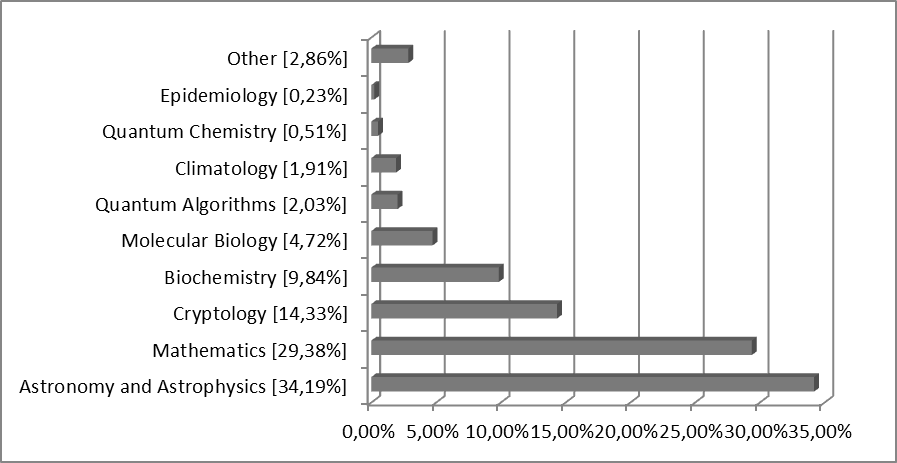
\includegraphics[width=10cm]{104_2013_w_Swierczewski_boinc_1}
  \caption{The division of all credits granted by BOINC in terms of scientific disciplines which concern the calculation.}\label{fig:swier1}
\end{figure}

An interesting alternative to centralized supercomputers is BOINC. BOINC (\cite{swier1}) is a system enabling use of personal computers for scientific research, and so, it can be considered as the the way to crowdsource scientific calculations. It allows to carry out calculations on a large scale incurring minimal costs associated with the purchase of equipment and its operation. In the case of BOINC infrastructure, as administrators we are forced to take care only of servers, which send computing tasks to the computers of individuals who have agreed to use their machines in his spare time to performed calculations for the good of science.

The user attaching to BOINC can choose one or several projects, in which he or she wishes to participate. The choice is very wide and covers many scientific fields from the mathematics and astrophysics to biochemistry. List of the best-known projects includes, among others, World Community Grid (\cite{swier2}). WCG is funded and managed by IBM. By providing the computing power of your PC in this project it contributes into, for example, the development of AIDS research, or into search of treatment for schistosomiasis. The LHC@Home (\cite{swier3}), which supports the project Large Hadron Collider (LHC), is also worth mentioning. One of the CERN department  decided to use BOINC to simulate the behavior of particles orbiting in the accelerator which allows to study the stability of their trajectory. During the test on each machine simulates the most common trip 60 particles around the ring by 100 000 laps.

\begin{figure}[h]
  \centering
  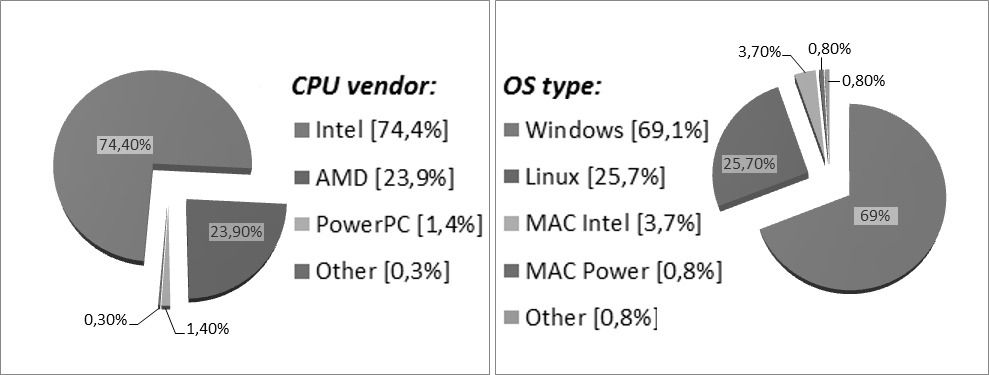
\includegraphics[width=10cm]{104_2013_w_Swierczewski_boinc_2}
  \caption{Operating systems and processors of the BOINC users.}\label{fig:swier2}
\end{figure}


After registration, the BOINC and calculated in the selected pro\-ject's first tasks, you will receive points. They are to some extent paid for their input in the development of science.
Number of points owned by the user should reflect how much time user's computers are dedicated to solving computational tasks. Fig.~\ref{fig:swier1} presents the percentage of all points in the various fields of science. It is seen, that projects for Astronomy and Astrophysics are the most popular ones. Second place belongs to the queen of sciences, i.e. to mathematics. Distribution of points over  nationalities is a special subject of interest. First position in terms of participation in BOINC belongs to Americans, of course, who have a significant advantage over Germans. The top five includes also England, Japan and France. This comparison is presented in Fig.~\ref{fig:swier3}. Fig.~\ref{fig:swier2} presents a summary on used processors and operating systems. Linux operating system has a relatively large group of users here "--- up to 25.70\%.

\begin{figure}[h]
  \centering
  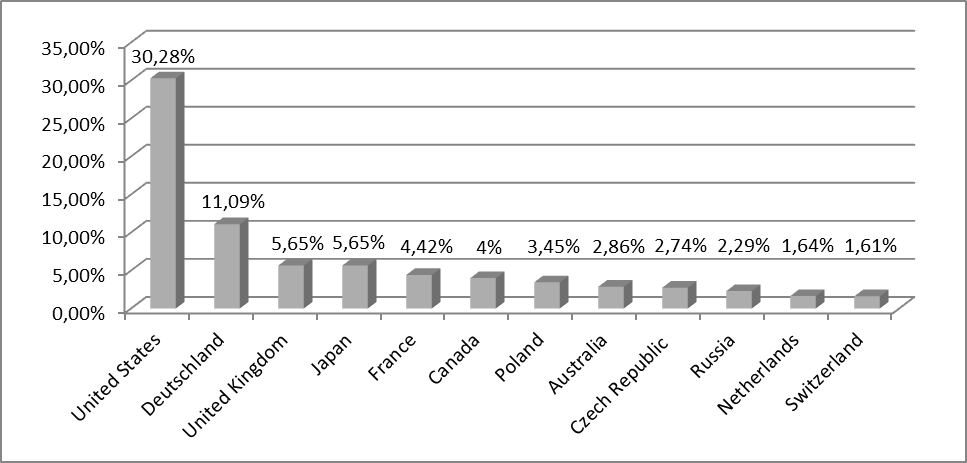
\includegraphics[width=10cm]{104_2013_w_Swierczewski_boinc_3}
  \caption{The country ranking in terms of quantity calculations carried out by members of the appropriate nationality.}\label{fig:swier3}
\end{figure}

Certainly it can be concluded that BOINC platform as a solution is worth of attention even for those who have no connection with science.

With this kind of initiatives we can make something significant for our common civilization.

\begin{thebibliography}{9}
\bibitem{swier1} BOINC homepage: \url{http://boinc.berkeley.edu/}
\bibitem{swier2} World Community Grid website: \url{http://www.worldcommunitygrid.org/}
\bibitem{swier3} LHC@Home website: \url{http://lhcathome.web.cern.ch/LHCathome/}
\end{thebibliography}

\end{document}

\documentclass[10pt, a5paper]{article}
\usepackage{pdfpages}
\usepackage{parallel}
\usepackage[T2A]{fontenc}
\usepackage{ucs}
\usepackage[utf8x]{inputenc}
\usepackage[polish,english,russian]{babel}
\usepackage{hyperref}
\usepackage{rotating}
\usepackage[inner=2cm,top=1.8cm,outer=2cm,bottom=2.3cm,nohead]{geometry}
\usepackage{listings}
\usepackage{graphicx}
\usepackage{wrapfig}
\usepackage{longtable}
\usepackage{indentfirst}
\usepackage{array}
\newcolumntype{P}[1]{>{\raggedright\arraybackslash}p{#1}}
\frenchspacing
\usepackage{fixltx2e} %text sub- and superscripts
\usepackage{icomma} % коскі ў матэматычным рэжыме
\PreloadUnicodePage{4}

\newcommand{\longpage}{\enlargethispage{\baselineskip}}
\newcommand{\shortpage}{\enlargethispage{-\baselineskip}}

\def\switchlang#1{\expandafter\csname switchlang#1\endcsname}
\def\switchlangbe{
\let\saverefname=\refname%
\def\refname{Літаратура}%
\def\figurename{Іл.}%
}
\def\switchlangen{
\let\saverefname=\refname%
\def\refname{References}%
\def\figurename{Fig.}%
}
\def\switchlangru{
\let\saverefname=\refname%
\let\savefigurename=\figurename%
\def\refname{Литература}%
\def\figurename{Рис.}%
}

\hyphenation{admi-ni-stra-tive}
\hyphenation{ex-pe-ri-ence}
\hyphenation{fle-xi-bi-li-ty}
\hyphenation{Py-thon}
\hyphenation{ma-the-ma-ti-cal}
\hyphenation{re-ported}
\hyphenation{imp-le-menta-tions}
\hyphenation{pro-vides}
\hyphenation{en-gi-neering}
\hyphenation{com-pa-ti-bi-li-ty}
\hyphenation{im-pos-sible}
\hyphenation{desk-top}
\hyphenation{elec-tro-nic}
\hyphenation{com-pa-ny}
\hyphenation{de-ve-lop-ment}
\hyphenation{de-ve-loping}
\hyphenation{de-ve-lop}
\hyphenation{da-ta-ba-se}
\hyphenation{plat-forms}
\hyphenation{or-ga-ni-za-tion}
\hyphenation{pro-gramming}
\hyphenation{in-stru-ments}
\hyphenation{Li-nux}
\hyphenation{sour-ce}
\hyphenation{en-vi-ron-ment}
\hyphenation{Te-le-pathy}
\hyphenation{Li-nux-ov-ka}
\hyphenation{Open-BSD}
\hyphenation{Free-BSD}
\hyphenation{men-ti-on-ed}
\hyphenation{app-li-ca-tion}

\def\progref!#1!{\texttt{#1}}
\renewcommand{\arraystretch}{2} %Іначай формулы ў матрыцы зліпаюцца з лініямі
\usepackage{array}

\def\interview #1 (#2), #3, #4, #5\par{

\section[#1, #3, #4]{#1 -- #3, #4}
\def\qname{LVEE}
\def\aname{#1}
\def\q ##1\par{{\noindent \bf \qname: ##1 }\par}
\def\a{{\noindent \bf \aname: } \def\qname{L}\def\aname{#2}}
}

\def\interview* #1 (#2), #3, #4, #5\par{

\section*{#1\\{\small\rm #3, #4. #5}}

\def\qname{LVEE}
\def\aname{#1}
\def\q ##1\par{{\noindent \bf \qname: ##1 }\par}
\def\a{{\noindent \bf \aname: } \def\qname{L}\def\aname{#2}}
}

\begin{document}
\title{Обучение Linux в корпоративном секторе}
\author{Денис Пынькин, Владимир Шахов\footnote{Минск, Беларусь; \url{d4s@t-linux.by}, \url{lumpen.intellectual@gmail.com}}}
\maketitle
\begin{abstract}
Article describes gaps and problems of Linux in high school education and initiatives of commercial companies Epam and SaM Solutions in this area. Different approaches and different local targets but common understanding of problem and \linebreak cooperation in the spirit of Free Software.
\end{abstract}
\subsubsection*{Кризис в отрасли}

ОС Linux устойчиво набирает популярность в качестве платформы для разработки. Соответственно растет и количество коммерческих проектов с использованием этой операционной системы. Примерно в 2010-12 годах стало заметно невооруженным взглядом, что людей, знакомых с полным циклом разработки
для Linux-платформы, в особенности для встраиваемых и серверных ее применений, не так уж много. Хотя более правильным было бы сказать, что таких людей катастрофически не хватает для покрытия нужд белорусских IT компаний.

Основные проблемы обучения в ВУЗах РБ:

\begin{itemize}
  \item существует направленность на изучение закрытого стека технологий на основе ОС Windows, при этом применение Linux зависит исключительно от отдельных лиц, работающих в учебном заведении \cite{bib1};
  \item еще одна проблема прямо заложена в учебных планах, направленных на изучение теории, что приводит к самостоятельному освоению инструментальных средств программирования учащимися, которое, как правило, заканчивается на минимальном уровне владения выбранным (или навязанным) IDE;
  \item “классическое” обучение практически не затрагивает практики командной разработки с выделением в отдельные процессы собственно самой разработки, тестирования и развертывания ПО;
  \item преподавателями, в основной своей массе, совершенно игнорируются подходы, принятые в мире, связанном со Свободным ПО \cite{bib2}.
\end{itemize}

Кроме того отдельно хотелось бы отметить проблему закрытости и кастовости, распространенной в сообществе пользователей и разработчиков Linux, что никак не способствует привлечению новых членов.

Все эти проблемы приводят к тому, что разработчики, тестировщики и, в меньшей степени, администраторы, умеющие работать и знающие ОС Linux “самозарождаются”, что  является сравнительно медленным процессом и совершенно не подходит для коммерческих компаний.

По сути, на данный момент можно говорить, что экосистема вокруг ОС Linux в РБ отсутствует, а небольшие очаги притяжения акцентируются в первую очередь на вопросах администрирования и веб-разработки. Заметным исключением здесь является ежемесячная линуксовка, организованная в рамках Minsk Linux User Group при поддержке SaM Solutions, в рамках которой встречаются и обмениваются опытом наиболее активные представители разработчиков под ОС Linux.

\subsubsection*{EPAM, Embedded Solutions Department}

Принципиальное решение о необходимости дополнительного\linebreak привлечения молодых разработчиков к ОС Linux было принято в рамках департамента в начале 2012 года. Учитывая большой опыт компании по работе с учебными заведениями в РБ и острую необходимость в увеличении количества разработчиков для встраиваемых и серверных применений, уже осенью была оборудована совместная лаборатория Epam и БГУИР на базе кафедры ЭВМ КСиС и прошел первый набор слушателей на курсы по изучению ОС Linux для разработчиков.

Учитывая, что основная целевая аудитория курса --- студенты технических специальностей, была разработана программа, рассчитанная на людей, уже умеющих программировать на каком-либо языке, но желающих получить навыки разработки в среде ОС Linux. В программу курса вошли технологии и знания, помогающие адаптироваться к целевой платформе обучения.
В связи с ориентацией департамента на разработку серверных и встраиваемых решений, было принято решение не затрагивать работу и разработку в графическом окружении, а сконцентрироваться на работе в командной строке.
Сама программа разделена на 3 отдельных модуля:

\begin{itemize}
  \item введение в GNU/Linux --- минимальный набор знаний об архитектуре и особенностях работы в среде ОС Linux;
  \item программирование на bash --- разработчики рано или поздно сталкиваются с необходимостью разбираться в чужих скриптах, создавать свои, а также автоматизировать свою работу;
  \item инструментарий разработчика --- в этот модуль входят принципы разработки в ОС Linux, методы и навыки работы с классическими инструментами, такими как: компилятор, управление сборкой, установкой и распространением приложения, совместная работа с исходным кодом, анализ исполняемого файла и его работы, а также другие средства и подходы применяющиеся при разработке.
\end{itemize}

Курс читается не профессиональными лекторами, а разработчиками департамента, постоянно применяющими многие из изучаемых технологий на практике.

После успешного окончания курса слушателям будут вручены сертификаты о прохождении, а лучшим учащимся будет предложена работа в Epam в качестве разработчиков серверных и встраиваемых решений.

\subsubsection*{SaM Solutions, Linux \& Embedded department}

Внутренняя обучающая программа опирается на бизнес-план развития отдела Linux \& Embedded компании SaM Solutions, разработанный и принятый в 2011 году. Анализ рынка труда дал очень печальную картину крайней нехватки готовых специалистов с одной стороны и увеличения количества заказов с другой стороны. В качестве одной из мер по преодолению кадрового голода была предложена долговременная стратегия подготовки собственных кадров.

В декабре 2012 года был набран первый поток стажёров из 10 человек на специализацию Linux QA. Конкурс составил 3 человека на место. Учебная программа сформирована с учётом задач, решаемых на коммерческих проектах компании и направлена на максимально быстрый старт стажёров в качестве Junior QA Engineer.

Целевая аудитория -- взрослые люди любого возраста. Имеющие как профильное, так и непрофильное образование, желающие далее заниматься Linux в профессиональной сфере.

Как показал наш предшествующий опыт, успешный вход новых сострудников на эту специализацию прямо зависит от владения инструментарием Linux-систем. Никакие предшествующие курсы абстрактного QA в этом не помогают.

Программа обучения разбита на изолированные блоки по темам. Каждый блок может быть прочитан отдельно и заранее предусматривается повторное использование учебного материала. Как для будующих стажировок, так и внутренних занятий повышения квалификации.
Акцент сделан на инструментальной среде Linux в проекции на наши задачи по разработке коммерческих продуктов в части тестирования качества. А именно:

\begin{itemize}
  \item краткое введение в архитектуру
  \item работа в Shell: интерактивная и скриптование
  \item организация файловой системы
  \item подсистема управления процессами
  \item обработка текста (включая регулярные выражения)
  \item инструменты виртуализации
  \item базовые сведения об администрировании
  \item кратко об отладке приложений
\end{itemize}

Помимо стажёров к занятиям привлекаются вольнопосещающие из числа сотрудников компании. Занятия проводятся профильными специалистами отдела.

Есть планы подготовки подобных курсов по Linux Kernel Programming и Linux User-space Programming.

Сертификаты о прохождении пока не вручаются. От сотрудничества с официозными образовательными учреждениями мы отказались, в основном в силу организационных сложностей.

\subsubsection*{Совместная работа}

На данный момент существует общая стратегическая задача, как Linux сообщества, так и корпоративного сектора --- это создание широкой и устойчивой экосистемы, связанной с ОС Linux в среде IT-специалистов и желающих стать таковыми.

В процессе роста сообщества, увеличивается не просто количество технических специалистов, кроме того, увеличивается количество людей знающих и разделяющих ценности, заложенные в принципах Свободного ПО.
Интерес компаний очевиден, ведь  именно из этого сообщества приходят так необходимые для коммерческой разработки профессионалы.

Учитывая специфику области, в профильных департаментах\linebreak независимо друг от друга было принято решение вести максимально возможно открытую политику обучения.
В первую очередь это привело в неформальной договоренности о создании совместных материалов с открытым доступом для обучения.

Таким образом на github появился открытый проект, содержащий на первом этапе лекционные слайды, которые добавляются по мере создания: \url{https://github.com/d4s/linux\_courses/network/members} или \url{https://github.com/SaM-Solutions/linux\_courses/network/members/}. Отдельно хотелось бы отметить, что благодаря такому подходу у любого заинтересованного лица --- будь то представитель другой компании, либо студент, есть возможность участвовать в процессе обучения, корректировать материалы и создавать новые, а также проводить свои собственные курсы, используя уже созданные материалы.

В своем роде --- это уникальный для просторов РБ проект с открытым исходным кодом.

\subsubsection*{Что дальше?}

Поскольку курсы все еще продолжаются, первый итоги первого этапа будут подведены позже, но уже сейчас можно сказать, что потребуется унификация материалов.

Кроме того, авторы очень надеются, что кроме каталогов “epam” и “sam-solutions” в репозитории с исходниками появятся каталоги с названиями других компаний, заинтересованных в развитии экосистемы вокруг ОС Linux.

\begin{thebibliography}{9}
\bibitem{bib1} {Derechennik S.S., Kostiuk D.A., Pynkin D.A. Free/libre software usage in the belarusian system of higher educational institutions // Друга міжнародна науково-практична конференція FOSS Lviv-2012: Збірник наукових праць/ Львів, 26-28 квітня 2012 р.}
\bibitem{bib2} {Д.А. Пынькин, И.И. Глецевич. Открытый подход к обучению студентов технической
специальности ВУЗа // 7-я конференция «СПО в высшей школе»: Тезисы докладов. \url{http://freeschool.altlinux.ru/wp-content/uploads/2012/01/pereslavl-winter-2012.pdf}}\end{thebibliography}
\end{document}

\documentclass[10pt, a5paper]{article}
\usepackage{pdfpages}
\usepackage{parallel}
\usepackage[T2A]{fontenc}
\usepackage{ucs}
\usepackage[utf8x]{inputenc}
\usepackage[polish,english,russian]{babel}
\usepackage{hyperref}
\usepackage{rotating}
\usepackage[inner=2cm,top=1.8cm,outer=2cm,bottom=2.3cm,nohead]{geometry}
\usepackage{listings}
\usepackage{graphicx}
\usepackage{wrapfig}
\usepackage{longtable}
\usepackage{indentfirst}
\usepackage{array}
\newcolumntype{P}[1]{>{\raggedright\arraybackslash}p{#1}}
\frenchspacing
\usepackage{fixltx2e} %text sub- and superscripts
\usepackage{icomma} % коскі ў матэматычным рэжыме
\PreloadUnicodePage{4}

\newcommand{\longpage}{\enlargethispage{\baselineskip}}
\newcommand{\shortpage}{\enlargethispage{-\baselineskip}}

\def\switchlang#1{\expandafter\csname switchlang#1\endcsname}
\def\switchlangbe{
\let\saverefname=\refname%
\def\refname{Літаратура}%
\def\figurename{Іл.}%
}
\def\switchlangen{
\let\saverefname=\refname%
\def\refname{References}%
\def\figurename{Fig.}%
}
\def\switchlangru{
\let\saverefname=\refname%
\let\savefigurename=\figurename%
\def\refname{Литература}%
\def\figurename{Рис.}%
}

\hyphenation{admi-ni-stra-tive}
\hyphenation{ex-pe-ri-ence}
\hyphenation{fle-xi-bi-li-ty}
\hyphenation{Py-thon}
\hyphenation{ma-the-ma-ti-cal}
\hyphenation{re-ported}
\hyphenation{imp-le-menta-tions}
\hyphenation{pro-vides}
\hyphenation{en-gi-neering}
\hyphenation{com-pa-ti-bi-li-ty}
\hyphenation{im-pos-sible}
\hyphenation{desk-top}
\hyphenation{elec-tro-nic}
\hyphenation{com-pa-ny}
\hyphenation{de-ve-lop-ment}
\hyphenation{de-ve-loping}
\hyphenation{de-ve-lop}
\hyphenation{da-ta-ba-se}
\hyphenation{plat-forms}
\hyphenation{or-ga-ni-za-tion}
\hyphenation{pro-gramming}
\hyphenation{in-stru-ments}
\hyphenation{Li-nux}
\hyphenation{sour-ce}
\hyphenation{en-vi-ron-ment}
\hyphenation{Te-le-pathy}
\hyphenation{Li-nux-ov-ka}
\hyphenation{Open-BSD}
\hyphenation{Free-BSD}
\hyphenation{men-ti-on-ed}
\hyphenation{app-li-ca-tion}

\def\progref!#1!{\texttt{#1}}
\renewcommand{\arraystretch}{2} %Іначай формулы ў матрыцы зліпаюцца з лініямі
\usepackage{array}

\def\interview #1 (#2), #3, #4, #5\par{

\section[#1, #3, #4]{#1 -- #3, #4}
\def\qname{LVEE}
\def\aname{#1}
\def\q ##1\par{{\noindent \bf \qname: ##1 }\par}
\def\a{{\noindent \bf \aname: } \def\qname{L}\def\aname{#2}}
}

\def\interview* #1 (#2), #3, #4, #5\par{

\section*{#1\\{\small\rm #3, #4. #5}}

\def\qname{LVEE}
\def\aname{#1}
\def\q ##1\par{{\noindent \bf \qname: ##1 }\par}
\def\a{{\noindent \bf \aname: } \def\qname{L}\def\aname{#2}}
}


\begin{document}
\title{F/LOSS for Open Science: Crystallography Open Database}
\author{Saulius Gražulis \footnote{Vilnius, Lithuania}}
\maketitle
\begin{abstract}
Free and Open Source software serves both as a model of development and as enabling methodology for many other fields of human enterprise. We have applied the Free software and Open source principles to create an open access scientific database in the field of chemical crystallography.
\end{abstract}
The COD project (abbreviated from the `Crystallography Open Database', \url{http://www.crystallography.net/}) aims at collecting in a single open access database all organic, inorganic and metal organic structures \cite{graz1} (except for the structures of biological macromolecules that are available at the PDB \cite{graz2}). The database was founded by Armel Le Bail, Lachlan Cranswick, Michael Berndt, Luca Lutterotti and Robert M. Downs in February 2003 as a response to Michael Berndt’s letter published in the Structure Determination by Powder Diffractometry (SDPD) mailing list \cite{graz3}. Since December 2007 the main database server is maintained and new software is developed in the Vilnius University Institute of Biotechnology by Saulius Gražulis and Andrius Merkys, and has now over 200 thousand records describing structures published in major crystallographic and chemical peer"=reviewed journals \cite{graz4}.

The COD database is implemented using F/LOSS software, on a LAMP platform, with addition of the home made Linux command line software licensed under GPL. The database itself is also governed using open principles: access to data is free (as in freedom) to all who would wish it, and deposition of data is open for all registered users, given the data they provide meet quality criteria accepted in science. In future, we plan to implement a Web based peer-review network, enabling new, open ways of doing science. We expect a considerable synergy from application of open source principles in combination with scientific merits.

\begin{thebibliography}{9}
\bibitem{graz1} Gražulis, S.; Chateigner, D.; Downs, R. T.; Yokochi, A. F. T.; Quirós, M.; Lutterotti, L.; Manakova, E.; Butkus, J.; Moeck, P. \& Le Bail, A. (2009). Crystallography Open Database – an open-access collection of crystal structures, Journal of Applied Crystallography 42: 726--729.
\bibitem{graz2} Berman, H.; Henrick, K. \& Nakamura, H. (2003). Announcing the worldwide Protein Data Bank, Nat Struct Mol Biol 10: 980--980.
\bibitem{graz3} Berndt, M. (2003). Open crystallographic database "--- a role for whom?, \url{http://tech.groups.yahoo.com/group/sdpd/message/1016} (retrieved 2013.01.31).
\bibitem{graz4} Gražulis, S.; Daškevič, A.; Merkys, A.; Chateigner, D.; Lutterotti, L.; Quirós, M.; Serebryanaya, N. R.; Moeck, P.; Downs, R. T. \& Le Bail, A. (2012). Crystallography Open Database (COD): an open-access collection of crystal structures and platform for world-wide collaboration, Nucleic Acids Research 40: D420--D427.
\end{thebibliography}

\end{document}

\documentclass[10pt, a5paper]{article}
\usepackage{pdfpages}
\usepackage{parallel}
\usepackage[T2A]{fontenc}
\usepackage{ucs}
\usepackage[utf8x]{inputenc}
\usepackage[polish,english,russian]{babel}
\usepackage{hyperref}
\usepackage{rotating}
\usepackage[inner=2cm,top=1.8cm,outer=2cm,bottom=2.3cm,nohead]{geometry}
\usepackage{listings}
\usepackage{graphicx}
\usepackage{wrapfig}
\usepackage{longtable}
\usepackage{indentfirst}
\usepackage{array}
\newcolumntype{P}[1]{>{\raggedright\arraybackslash}p{#1}}
\frenchspacing
\usepackage{fixltx2e} %text sub- and superscripts
\usepackage{icomma} % коскі ў матэматычным рэжыме
\PreloadUnicodePage{4}

\newcommand{\longpage}{\enlargethispage{\baselineskip}}
\newcommand{\shortpage}{\enlargethispage{-\baselineskip}}

\def\switchlang#1{\expandafter\csname switchlang#1\endcsname}
\def\switchlangbe{
\let\saverefname=\refname%
\def\refname{Літаратура}%
\def\figurename{Іл.}%
}
\def\switchlangen{
\let\saverefname=\refname%
\def\refname{References}%
\def\figurename{Fig.}%
}
\def\switchlangru{
\let\saverefname=\refname%
\let\savefigurename=\figurename%
\def\refname{Литература}%
\def\figurename{Рис.}%
}

\hyphenation{admi-ni-stra-tive}
\hyphenation{ex-pe-ri-ence}
\hyphenation{fle-xi-bi-li-ty}
\hyphenation{Py-thon}
\hyphenation{ma-the-ma-ti-cal}
\hyphenation{re-ported}
\hyphenation{imp-le-menta-tions}
\hyphenation{pro-vides}
\hyphenation{en-gi-neering}
\hyphenation{com-pa-ti-bi-li-ty}
\hyphenation{im-pos-sible}
\hyphenation{desk-top}
\hyphenation{elec-tro-nic}
\hyphenation{com-pa-ny}
\hyphenation{de-ve-lop-ment}
\hyphenation{de-ve-loping}
\hyphenation{de-ve-lop}
\hyphenation{da-ta-ba-se}
\hyphenation{plat-forms}
\hyphenation{or-ga-ni-za-tion}
\hyphenation{pro-gramming}
\hyphenation{in-stru-ments}
\hyphenation{Li-nux}
\hyphenation{sour-ce}
\hyphenation{en-vi-ron-ment}
\hyphenation{Te-le-pathy}
\hyphenation{Li-nux-ov-ka}
\hyphenation{Open-BSD}
\hyphenation{Free-BSD}
\hyphenation{men-ti-on-ed}
\hyphenation{app-li-ca-tion}

\def\progref!#1!{\texttt{#1}}
\renewcommand{\arraystretch}{2} %Іначай формулы ў матрыцы зліпаюцца з лініямі
\usepackage{array}

\def\interview #1 (#2), #3, #4, #5\par{

\section[#1, #3, #4]{#1 -- #3, #4}
\def\qname{LVEE}
\def\aname{#1}
\def\q ##1\par{{\noindent \bf \qname: ##1 }\par}
\def\a{{\noindent \bf \aname: } \def\qname{L}\def\aname{#2}}
}

\def\interview* #1 (#2), #3, #4, #5\par{

\section*{#1\\{\small\rm #3, #4. #5}}

\def\qname{LVEE}
\def\aname{#1}
\def\q ##1\par{{\noindent \bf \qname: ##1 }\par}
\def\a{{\noindent \bf \aname: } \def\qname{L}\def\aname{#2}}
}

\def\vv!#1!{\texttt{#1}}
\def\fakeparagraph#1{\textbf{#1}}
\begin{document}
\title{Алгарытмы паляпшэння выяваў у ВПЗ: падаўленне шумоў}
\author{Антон Літвіненка \footnote{Кіеў, Ukraine}}
\maketitle
\begin{abstract}
A review of image denoising enhancement algorithms devilered by FLOSS projects is provided together with discussion of their end-user characteristics and some theoretical aspects.
\end{abstract}
Лічбавая апрацоўка выяваў дазваляе паляпшэнне іх якасці, ў прыватнасці ў выпадку, калі тэхнічныя магчымасці фотаапаратуры (ці іншых сродкаў атрымання выявы) не дазваляюць атрымання якаснага выніку адразу, альбо ж з любых іншых прычынаў не атрымалася стварыць выяву належнае якасці.

Тэарэтычныя засады працэсу паляпшэння выяваў грунтуюцца на тэорыі хібнасцяў, тэорыі інфармацыі ды тэорыях чалавечаскага зроку. Варта мець на ўвазе наступныя палажэнні:

\begin{enumerate}
  \item Канчатковай мэтай працэсу паляпшэння якасці з’яўляецца атрыманне выявы, якая ўспрымалася б чалавечым зрокам як больш дасканалая ў параўнанні з арыгіналам. Такім чынам, фармальныя крытэры (зашумленасць, наяўнасць артэфактаў ці скажэнняў і г.~д.) з’яўляюцца выключна дапаможнымі (і выяўленне іх сувязі з успрыйняццём чалавечаскім зрокам з’яўляецца нетрывіяльнай задачай навукі і мастацтва). Напрыклад, празмернае падаўленне шуму можа прывесці да горшага выніку  («пластмасавы твар»), чым частковае.
  \item Недахопы выявы, як правіла, маюць пэўны ўзор, які дазваляе адрозніць іх ад карыснай інфармацыі паводле фармальных крытэраў, якія могуць вылічацца праграмна ў аўтаматычным ці напаўаўтаматычным рэжыме. Напрыклад, г.~зв. «гарачыя пікселы» (дэфектныя элементы матрыцы) рэзка адрозніваюцца ад суседзяў "--- як правіла, маюць максімальнае значэнне ў адным канале RGB (ці ў некалькіх).
  \item Алгарытмы паляпшэння бяруць усю неабходную інфармацыю для пабудовы выніковага здымку выключна з арыгінальнай выявы. Калі гэтая інфармацыя фізічна адсутнічае, паляпшэнне немагчымае (з выявы $100\times100$ немагчыма зрабіць стэнд А0).
  \item Тым не менш, пэўная колькасць карыснай інфармацыі заўсёды губляецца ў працэсе паляпшэння.
\end{enumerate}

\subsection*{Выдаленне шумоў}

У сучаснай фатаграфіі асноўным аб’ектам выдалення шумоў з’яўляецца цеплавы шум сенсара (лічбавых камер альбо сканераў). Выкарыстанне высокіх значэнняў святлоадчувальнасці ды неабходнасць асвятляць цёмныя фрагменты выявы робяць шумы даволі заўважнымі. Узор такога шуму "--- невялікія выпадковыя адхіленні ад «правільных» значэнняў з пэўным статыстычным размеркаваннем.

\begin{itemize}
  \item Лічбавы шум з’яўляецца каляровым і даволі непрыемным на выгляд;
  \item У кампактных камерах з няпоўным (\emph{cropped}) кадрам заўважны шум можа пачынацца на ISO 200, а ў найпрасцейшых "--- нават на ISO 100.
  \item Для чалавечаскага вока монахромны шум выглядае прыемней каляровага, таму падаўленне шума можа прымяняцца толькі да інфармацыі пра колер піксела (як правіла, ў каляровай прасторы LAB), пакідаючы некранутай інфармацыю пра яркасць.
  \item Часам карыстальнікі блытаюць лічбавы шум і зярно плёнкі, з якім зараз амаль не даводзіцца мець справу праз высокую якасць сучаснай плёнкі (шумы сканера мацнейшыя) і эстэтычны выгляд самаго зярна (для прыгажосці здымку прыбраць шум важней, чым зярно).
  \item Любая інфармацыя, якая абмяжоўвае агульнасць ўзору шумоў, можа і мусіць выкарыстоўвацца. Напрыклад, у сканах каляровых негатываў C-41  большасць шумоў хаваецца ў сінім канале схемы RGB (шмат сканэраў, у прыватнасці планшэтных, маюць праблемы з «выцягваннем» дадзеных сіняга каналу праз інтэнсіўную аранжавую маску на негатывах C-41) "--- мэтазгодна прыбіраць шумы ў першую чаргу ў ім.
\end{itemize}

Далей будзе разглянуты шэраг алгарытмаў для выдалення шумоў з выявы і іх рэалізацыю ў вольных праграмных прадуктах: \href{http://www.gimp.org/}{GIMP} (GPL3+), \href{http://www.imagemagick.org/}{ImageMagick} (Apache 2.0), \href{http://gmic.sourceforge.net/}{G'MIC} (+ранейшая\linebreak {GREYCStoration}, CeCILL license), \href{http://krita.org/}{Krita} (GPL2), \href{http://ufraw.sourceforge.net/}{ufraw} (GPL).

\subsubsection*{Алгарытмы (для цеплавога шуму без «гарачых пікселаў» ды плямаў)}

\fakeparagraph{Размыццё (прымітыўны).}
Гаўсава размыццё + памяншэнне памеру. Вельмі просты, але губляецца шмат інфармацыі. Можа быць карысны пры нестандартных узорах шумоў, калі падабраць больш прасунуты спосаб падаўлення не атрымліваецца. Даступны ў любым рэдактары.

Прыклад для {ImageMagick}:\\
\texttt{newsize=`convert src.tif -format "\%[fx:w/4]x\%[fx:h/4]" info:`}
\texttt{convert src.tif -blur 4x4 -resize \$newsize dst.tif}

\fakeparagraph{Dechroma.}
Гаўсава размыццё каляровых каналаў A і B у схеме LAB з вялікім радыюсам (15--100). Робіць шум монахраматычным. Змяшчае каляровую гаму выявы (як правіла, пасля апрацоўкі даводзіцца дадаць чырвані). Можа быць карысны як адзін з пунктаў апрацоўкі пры моцнай зашумленасці выявы альбо як адзіны пры невялікім каляровым шуме (калі з нейкіх прычынаў непажадана кранаць канал яркасці). Даступны ў любым рэдактары, здольным працаваць са схемай LAB (у {GIMP} рэалізаваны як асобны плагін {dechroma}).

\fakeparagraph{GREYCStoration (анізатропнае згладжванне).}
Алгарытм, \linebreak заснаваны на выкарыстанні дыфэренцыяльных ураўненняў у частковых вытворных для анізатропнага (з марфалагічным аналізам і захаваннем контураў) згладжвання (\cite{litvw1},\cite{litvw2}). Апрача падаўлення шумоў, можа выкарыстоўвацца для павялічэння памеру выявы (з аналізам марфалогіі ды тэкстурным сінтэзам для дадатковых пікселаў), а таксама для інтэрпаляцыі выявы (для выдалення пылу, надпісаў і г.~д.). У той жа час, не вельмі добра спраўляецца з моцна зашумленымі выявамі (атрымліваецца альбо «пластмасавая» выява, альбо застаюцца вялікія і хімерна пакручаныя (хаця і «выраўненыя») плямы).  Рэалізаваны як асобная праграма {GREYCStoration} (пазней увайшла у склад праэкту {G'MIC} як «anisotropic smoothing»)  і плагін для {GIMP} (як у межах {G'MIC для GIMP}, так і асобна).

\fakeparagraph{Wavelet denoise.}
Алгарытм, заснаваны на выкарыстанні вэйвлетнай апрацоўкі дадзеных. Выдзяляе элементы выявы розных характэрыстычных памераў, некаторыя аслабляючы (падаўленне шумоў), а некаторыя узмацняючы (падвышэнне рэзкасці).  Добра спраўляецца з шумамі рознай моцнасці. У той жа час, на моцна зашумленых выявах пакідае частку дэфектаў у выглядзе плямаў, падобных на вынік застасавання пудры. Апрача таго, троху мацней за GREYCStoration размывае выяву. Аптымальным з’яўляецца выкарыстанне на як мага ранейшым этапе апрацоўкі (напрыклад, выкарыстанне пры канверсіі RAW лепей ад выкарыстання пры апрацоўцы выніку канверсіі). Рэалізаваны ў {GIMP} (плагін), {Krita}, {ufraw}. Не рэалізаваны ў {ImageMagick} і {G'MIC}.

{Асабісты досвед аўтара ў большасці выпадкаў рэкамендуе выкарыстанне фільтра wavelet denoise з пошукам аптымальных наладак (магчыма, разам з падвышэннем рэзкасці выявы), у выпадках не вельмі зашумленых кадраў "--- таксама GREYCStoration.}

\subsubsection*{Плямы}
Гэты тып шумоў характэрызуецца тым, што значэнні пікселаў у іх цалкам выбіваюцца з шэрагу суседніх пікселаў і фрагментаў выявы, а пры тым ніяк не залежаць ад іх «правільных» значэнняў. Іх прычынай могуць быць, напрыклад: пыл і бруд на матрыцы ды оптыцы, «бітыя» і «гарачыя» пікселы (сапсаваныя элементы матрыцы), пыл і драпіны на плёнках, надпісы і «вадзяныя знакі» на выяве і г.~д. Агульны падыход да іх выдалення заключаецца ў знаходжанні закранутых плямай пікселаў ды іх заменай на пікселы, значэнні каторых пэўным чынам сінтэзаваныя з атачэння (гаўсавым размыццём ці метадамі аналізу марфалогіі). Галоўнай праблемай з’яўляецца правільны пошук і вызначэнне межаў плям (а таксама іх адрозненне ад «карысных» элементаў выявы). З гэтай мэтай ужываецца шмат спецыфічных падыходаў.

\fakeparagraph{Пошук крытычных значэнняў пікселаў.}
Крытычныя значэнні (блізкія да мінімальных ці максімальных) пікселаў нехарактэрныя для тыповай фатаграфіі ці малюнка (тыповы максімальны белы колер на фатаграфіі будзе не \vv!\#ffffff!, а нешта накшталт \vv!\#e5e5e5!), бо іначай фрагменты выявы могуць выглядаць як плямы перасветаў ці недасветаў. Таму пікселы са значэннямі вышэй і ніжэй пэўных гранічных разглядаюцца як ненатуральныя. Так працуе плагін «прыбраць плямы» ({despeckle}) для {GIMP}, прыбіранне «гарачых» пікселаў ва {ufraw} і {G'MIC}. У {Krita} ды {ImageMagick} непасрэдная рэалізацыя адсутнічае (хаця ўручную можна рэалізаваць падобны алгарытм у шматлікіх рэдактарах).

\fakeparagraph{Медыянныя фільтры.}
Базуюцца на ізаляванасці шуму і тым, што зашумленыя пікселы выбіваюцца з агульнага шэрагу. Для фрагмента пэўнага памеру вакол піксела вылічаецца медыяннае значэнне, якое замяшчае першаснае значэнне гэтага піксела. Пасля атрыманы вынік можа пэўным чынам змешвацца із зыходнай выявай. Рэалізавана ў {G'MIC} (ў тым ліку {G'MIC для Gimp}), у скрыпце {isonoise} \cite{litvw3} на базе {ImageMagick}.

\fakeparagraph{Чорны кадр.}
Застасоўваецца збольшага для апрацоўкі RAW. Праграме акрамя асноўнае выявы перадаецца выява, знятая пры тых жа ўсталяваннях, але ў поўнай цемры. Дазваляе вылучыць «бітыя» і «гарачыя» пікселы. Рэалізаваны ва {ufraw}.

\fakeparagraph{Інфрачырвоная падсветка.}
Пры сканаванні каляровых C-41 негатываў ці E-6 слайдаў робіцца дадатковы праход сканера з інфрачырвонай лампай, у святле якой праяўляюцца дэфекты плёнкі (пыл, драпіны). Рэалізавана ў шматлікіх праграмах для сканавання плёнкі (збольшага прапрыетарных). Не працуе для класічных (срэбных) чорна-белых плёнак.

\fakeparagraph{Штамп і healing brush.}
Павольны, але высакаякасны біямеханічны спосаб пошуку і выдалення плямаў. Рэалізаваны ў {GIMP}.\\

Нажаль, абмежаваныя досвед і поспехі аўтара на ніве ачысткі выяваў ад плям пакуль не дазваляюць надаць больш-менш агульныя рэкамендацыі на гэты конт.

Такім чынам, вольнае праграмнае забеспячэнне рэалізуе шырокі спектр магутных тэарэтычна абгрунтаваных алгарытмаў прыбірання шумоў з лічбавых выяваў, якія даюць карыстальніку вялікі выбар інструментаў для паляпшэння якасці выяваў, першасная якасць якіх з нейкай прычыны з’яўляецца недастатковай.

\begin{thebibliography}{9}
\bibitem{litvw1} D. Tschumperlé. Fast Anisotropic Smoothing of Multi-Valued Images using Curvature-Preserving PDE's, International Journal of Computer Vision, May 2006;
\bibitem{litvw2} D. Tschumperlé, R. Deriche. Vector-Valued Image Regularization with PDE's : A Common Framework for Different Applications. IEEE Transactions on Pattern Analysis and Machine Intelligence, Vol 27, No 4, pp 506-517, April 2005.
\bibitem{litvw3} Fred's ImageMagick Scripts: Isonoise. \url{http://www.fmwconcepts.com/imagemagick/isonoise/index.php}
\end{thebibliography}
\end{document}

\documentclass[10pt, a5paper]{article}
\usepackage{pdfpages}
\usepackage{parallel}
\usepackage[T2A]{fontenc}
\usepackage{ucs}
\usepackage[utf8x]{inputenc}
\usepackage[polish,english,russian]{babel}
\usepackage{hyperref}
\usepackage{rotating}
\usepackage[inner=2cm,top=1.8cm,outer=2cm,bottom=2.3cm,nohead]{geometry}
\usepackage{listings}
\usepackage{graphicx}
\usepackage{wrapfig}
\usepackage{longtable}
\usepackage{indentfirst}
\usepackage{array}
\newcolumntype{P}[1]{>{\raggedright\arraybackslash}p{#1}}
\frenchspacing
\usepackage{fixltx2e} %text sub- and superscripts
\usepackage{icomma} % коскі ў матэматычным рэжыме
\PreloadUnicodePage{4}

\newcommand{\longpage}{\enlargethispage{\baselineskip}}
\newcommand{\shortpage}{\enlargethispage{-\baselineskip}}

\def\switchlang#1{\expandafter\csname switchlang#1\endcsname}
\def\switchlangbe{
\let\saverefname=\refname%
\def\refname{Літаратура}%
\def\figurename{Іл.}%
}
\def\switchlangen{
\let\saverefname=\refname%
\def\refname{References}%
\def\figurename{Fig.}%
}
\def\switchlangru{
\let\saverefname=\refname%
\let\savefigurename=\figurename%
\def\refname{Литература}%
\def\figurename{Рис.}%
}

\hyphenation{admi-ni-stra-tive}
\hyphenation{ex-pe-ri-ence}
\hyphenation{fle-xi-bi-li-ty}
\hyphenation{Py-thon}
\hyphenation{ma-the-ma-ti-cal}
\hyphenation{re-ported}
\hyphenation{imp-le-menta-tions}
\hyphenation{pro-vides}
\hyphenation{en-gi-neering}
\hyphenation{com-pa-ti-bi-li-ty}
\hyphenation{im-pos-sible}
\hyphenation{desk-top}
\hyphenation{elec-tro-nic}
\hyphenation{com-pa-ny}
\hyphenation{de-ve-lop-ment}
\hyphenation{de-ve-loping}
\hyphenation{de-ve-lop}
\hyphenation{da-ta-ba-se}
\hyphenation{plat-forms}
\hyphenation{or-ga-ni-za-tion}
\hyphenation{pro-gramming}
\hyphenation{in-stru-ments}
\hyphenation{Li-nux}
\hyphenation{sour-ce}
\hyphenation{en-vi-ron-ment}
\hyphenation{Te-le-pathy}
\hyphenation{Li-nux-ov-ka}
\hyphenation{Open-BSD}
\hyphenation{Free-BSD}
\hyphenation{men-ti-on-ed}
\hyphenation{app-li-ca-tion}

\def\progref!#1!{\texttt{#1}}
\renewcommand{\arraystretch}{2} %Іначай формулы ў матрыцы зліпаюцца з лініямі
\usepackage{array}

\def\interview #1 (#2), #3, #4, #5\par{

\section[#1, #3, #4]{#1 -- #3, #4}
\def\qname{LVEE}
\def\aname{#1}
\def\q ##1\par{{\noindent \bf \qname: ##1 }\par}
\def\a{{\noindent \bf \aname: } \def\qname{L}\def\aname{#2}}
}

\def\interview* #1 (#2), #3, #4, #5\par{

\section*{#1\\{\small\rm #3, #4. #5}}

\def\qname{LVEE}
\def\aname{#1}
\def\q ##1\par{{\noindent \bf \qname: ##1 }\par}
\def\a{{\noindent \bf \aname: } \def\qname{L}\def\aname{#2}}
}


\def\vv!#1!{\texttt{#1}}
\begin{document}

\title{Etersoft Epm — универсальная оболочка управления пакетами}%\footnote{Текст данных и последующих тезисов, кроме специально оговоренных случаев, доступен под лицензией Creative Commons Attribution-ShareAlike 3.0}

\author{Даниил Михайлов, Виталий Липатов\footnote{Санкт-Петербург, Россия; \url{baraka@etersoft.ru}, url{lav@etersoft.ru}}}
\maketitle

\begin{abstract}
Epm is universal package manager for different Linux distributions and operating systems. Application and implementation details, which at the interface, similar to the rpm and apt at the same time, allows to perform necessary operations in a similar way on any platform.
\end{abstract}

EPM — универсальный пакетный менеджер, работающий на любых Linux"=платформах. Он позволяет решать основные задачи управления пакетами (установка, удаление, поиск) с помощью унифицированных команд. Для выполнения реальных действий выполняет команды пакетного менеджера, присущего конкретной системе.
Пример наиболее используемых команд:

%\begin{table}[t!]
%  \centering
  \begin{tabular}{l|p{2cm}|l|l}
    \hline
    Операция   & Нативная команда  & Команда epm & Сокращение \\
    \hline
    Установка  & \vv!apt-get install! \par \vv!urpmi! \par \vv!pacman -S! \par \vv!yum install! & \vv!epm install! & \vv!epmi! \\
    %\hline
    Удаление   & \vv!apt-get remove! \par \vv!urpme! \par \vv!pacman -R! \par yum remove! & \vv!epm remove! & \vv!epme! \\
    %\hline
    Поиск      & \vv!apt-cache search! \par \vv!urpmq -y! \par \vv!pacman -Ss! \par you search! & \vv!epm search! & \vv!epms! \\
    \hline
  \end{tabular}\\
%\end{table}

Управление пакетами тесно связано с управлением репозиториями пакетов (добавление, удаление, просмотр списка) и включением/выключением системных сервисов (так же устанавливаемых из пакетов). Эти действия так же унифицированы. Несколько команд для управления репозиториями на примере Mandriva:

%\begin{table}[h]
%  \centering
  \begin{tabular}{l|l|l}
    \hline
    Операция & Команда Mandriva & Команда epm \\
    \hline
    Список репозиториев & \vv!urpmq --list-url! & \vv!epm repolist! \\
    Добавить репозиторий & \vv!urpmi.addmedia! & \vv!epm addrepo! \\
    \hline
  \end{tabular}\\
%\end{table}

\pagebreak Примеры управления сервисами:

%\begin{table}[h]
%  \centering
  \begin{tabular}{l|l|l}
    \hline
    Операция & Команда Mandriva & Команда epm \\
    \hline
    Статус сервиса & \vv!service status! & \vv!cerv status! \\
    Старт сервиса & \vv!service start! & \vv!cerv addrepo! \\
    Автостарт & \vv!chkconfig on! & \vv!cerv on! \\
    \hline
  \end{tabular}\\
%\end{table}

EPM может использоваться при повседневном администрировании различных машин, в скриптах и средствах работы с пакетами. Скрипт, написанный с использованием epm, будет более гибким, сможет использоваться на разных системах производя установку пакетов и настройку сервисов.

EPM заменяет собой длинные справочники по командам различных пакетных менеджеров, обеспечивая администратору весь необходимый функционал управления пакетами даже для незнакомой системы, используя там команды с привычным синтаксисом: как apt в Debian, как rpm в Fedora, как urpm в Mandriva.

EPM уже сейчас поддерживает большое количество дистрибутивов: ALT Linux, Debian, Ubuntu, Mandriva, FreeBSD, Gentoo,\linebreak ArchLinux, Fedora, SUSE, Slackware. Большим преимуществом epm является простота расширения функционала и добавления поддерживаемых  дистрибутивов, с этой задачей справится любой желающий, знакомый с shell. Для добавления новой команды придется лишь найти файл, отвечающий за неё и дописать несколько строк на шелле.
Разумеется, возможность задания команд epm в синтаксисе любого из поддерживаемых дистрибутивов ограничена пересечениями (иногда две различные по смыслу команды из разных дистрибутивов имеют одинаковый синтаксис); в настоящий момент наиболее востребованные команды добавляются в epm по запросам пользователей в случае синтаксической совместимости с уже имеющимся функционалом.



\end{document}





\documentclass[10pt, a5paper]{article}
\usepackage{pdfpages}
\usepackage{parallel}
\usepackage[T2A]{fontenc}
\usepackage{ucs}
\usepackage[utf8x]{inputenc}
\usepackage[polish,english,russian]{babel}
\usepackage{hyperref}
\usepackage{rotating}
\usepackage[inner=2cm,top=1.8cm,outer=2cm,bottom=2.3cm,nohead]{geometry}
\usepackage{listings}
\usepackage{graphicx}
\usepackage{wrapfig}
\usepackage{longtable}
\usepackage{indentfirst}
\usepackage{array}
\newcolumntype{P}[1]{>{\raggedright\arraybackslash}p{#1}}
\frenchspacing
\usepackage{fixltx2e} %text sub- and superscripts
\usepackage{icomma} % коскі ў матэматычным рэжыме
\PreloadUnicodePage{4}

\newcommand{\longpage}{\enlargethispage{\baselineskip}}
\newcommand{\shortpage}{\enlargethispage{-\baselineskip}}

\def\switchlang#1{\expandafter\csname switchlang#1\endcsname}
\def\switchlangbe{
\let\saverefname=\refname%
\def\refname{Літаратура}%
\def\figurename{Іл.}%
}
\def\switchlangen{
\let\saverefname=\refname%
\def\refname{References}%
\def\figurename{Fig.}%
}
\def\switchlangru{
\let\saverefname=\refname%
\let\savefigurename=\figurename%
\def\refname{Литература}%
\def\figurename{Рис.}%
}

\hyphenation{admi-ni-stra-tive}
\hyphenation{ex-pe-ri-ence}
\hyphenation{fle-xi-bi-li-ty}
\hyphenation{Py-thon}
\hyphenation{ma-the-ma-ti-cal}
\hyphenation{re-ported}
\hyphenation{imp-le-menta-tions}
\hyphenation{pro-vides}
\hyphenation{en-gi-neering}
\hyphenation{com-pa-ti-bi-li-ty}
\hyphenation{im-pos-sible}
\hyphenation{desk-top}
\hyphenation{elec-tro-nic}
\hyphenation{com-pa-ny}
\hyphenation{de-ve-lop-ment}
\hyphenation{de-ve-loping}
\hyphenation{de-ve-lop}
\hyphenation{da-ta-ba-se}
\hyphenation{plat-forms}
\hyphenation{or-ga-ni-za-tion}
\hyphenation{pro-gramming}
\hyphenation{in-stru-ments}
\hyphenation{Li-nux}
\hyphenation{sour-ce}
\hyphenation{en-vi-ron-ment}
\hyphenation{Te-le-pathy}
\hyphenation{Li-nux-ov-ka}
\hyphenation{Open-BSD}
\hyphenation{Free-BSD}
\hyphenation{men-ti-on-ed}
\hyphenation{app-li-ca-tion}

\def\progref!#1!{\texttt{#1}}
\renewcommand{\arraystretch}{2} %Іначай формулы ў матрыцы зліпаюцца з лініямі
\usepackage{array}

\def\interview #1 (#2), #3, #4, #5\par{

\section[#1, #3, #4]{#1 -- #3, #4}
\def\qname{LVEE}
\def\aname{#1}
\def\q ##1\par{{\noindent \bf \qname: ##1 }\par}
\def\a{{\noindent \bf \aname: } \def\qname{L}\def\aname{#2}}
}

\def\interview* #1 (#2), #3, #4, #5\par{

\section*{#1\\{\small\rm #3, #4. #5}}

\def\qname{LVEE}
\def\aname{#1}
\def\q ##1\par{{\noindent \bf \qname: ##1 }\par}
\def\a{{\noindent \bf \aname: } \def\qname{L}\def\aname{#2}}
}


\begin{document}

\title{mkimage-profiles: долгая дорога в 0.9.x}%\footnote{Текст данных и последующих тезисов, кроме специально оговоренных случаев, доступен под лицензией Creative Commons Attribution-ShareAlike 3.0}

\author{Михаил Шигорин\footnote{Киев, Украина; \url{shigorin@gmail.com}}}
\maketitle

\begin{abstract}
The further development is discussed for mkimage-profiles, the tool that started as a research project to reduce configuration and code duplication while still being useful to those working on distribution images and virtual environments/machines. The overview of changes happening within and around mkimage"=profiles is presented for the period of about half a year while it is being prepared for production.
\end{abstract}

mkimage"=profiles изначально был <<домашним>> проектом по исследованию возможности уменьшения излишнего дублирования общей части конфигурации и вспомогательного кода, необходимого для формирования образов дистрибутивов и виртуальных окружений/машин \cite{Shigorinw1}.

Проект родился, подрос и начал выходить в мир. Ниже представлена попытка оценить характер и степень влияния изменений, происшедших в и около mkimage"=profiles за последние полгода при выведении его на начало реального применения.

За прошедшее время расширился список задач, усложнилась аппаратная часть, не стояла на месте подлежащая и соседняя инфраструктура, подключились новые люди. У проекта добавились документация в PDF, поддержка UEFI и первая боевая задача.

Из появившихся задач наиболее сложной, как ни странно, оказалась изначальная: облегчить жизнь релиз"=менеджеров и улучшить качество результата их труда. Обнаружилось, что коллегам нужны не только предусмотренные ранее и достаточно реализованные возможности, но и не совсем предполагавшиеся изначально или такие, которые сами по себе понятны, но нетривиальны в <<честной>> реализации.  Тем не менее спектр наработок, которые делают другие участники проекта, постепенно ширится, а в размышлениях над наиболее концептуально сложными моментами немало помог советом Н.Н. Непейвода.

К концу осени 2012 года была реализована начальная поддержка сборки UEFI"=совместимых образов, причём трудами Matthew Garrett получилось сделать их гибридными в квадрате --- usbflash/ \linebreak cdrom, BIOS/UEFI.  Из менее радикальных добавлений можно упомянуть поддержку APU и архитектуры armh (Sisyphus для ARM v7hf), а также добавление наборов firmware после ряда столкновений с реальным железом помимо тестовых виртуальных машин.

Набор функциональных <<кирпичиков>> также пополнился поддержкой основных DE и их форков.

Среди внешних изменений запомнились GNU Make 3.82, systemd"=197 и более локальные диверсии, производимые неизменно дружественными апстримами и коллегами по сизифу.

Документация оказалась в сложном положении: накопилось довольно много отдельных README"=файлов, разложенных по соответствующим <<закоулкам>> профиля и порой обновляемых (иногда даже внёсшим функциональность коммитом). Окинуть их все одним взглядом стало уже непросто. Выходом оказался некоторый race condition: из двух присланных альтернативных вариантов патчей после обсуждения был принят несколько более проработанный и минималистичный, превративший уже существующую документацию в asciidoc и добавивший её сборку в PDF и HTML.

Не обошлось и без разочарований: двое коллег из релиз"=менеджеров, более или менее плотно поработав с mkimage"=profiles \cite{Shigorinw2}, вернулись для текущих задач на привычные и тщательнее проработанные по критичным для них моментам mkimage"=profiles"=desktop, с доработки и рефакторинга которых собственно и начался этот проект.  Препятствием оказались две конкретные особенности (cleanup и i18n), недостатки по которым были уже известны и попытки решения которых прорабатывались, но на сей момент не приведены в приличный вид и, соответственно, не включены в основное дерево.

С другой стороны, для людей с более специфическими задачами mkimage"=profiles неожиданно оказался удобней: например, начальное портирование дистрибутива с озвучиванием ALT Linux Homeros было выполнено в течение одного"=двух дней.

Потенциал развития проекта далеко не исчерпан и списки todo полны как никогда, но при этом уже начинает просматриваться следующее поколение систем сборки, которому придёт время воплощаться через несколько лет.

Тем временем оказались полезными даже начальные результаты по первой <<настоящей>> задаче \cite{Shigorinw3}: в автоматическом режиме создан и опубликован набор из 18 <<живых>> установочных ISO"=образов (8 DE и icewm, i586/x86\_64±UEFI), позволивший разработчикам уже в процессе подготовки отловить ряд апстримных багов и межглючных взаимодействий и имеющий как минимум ещё одного настоящего пользователя со слишком новым ноутбуком, кроме вашего покорного слуги.  Эти сборки предполагается обновлять еженедельно, а при запросах майнтейнеров --- хоть ежедневно.

При проектировании mkimage-profiles было решено организовать инкрементальное построение конфигурации целевых образов на основе базовых дистрибутивов --- <<пустых>> инсталятора, livecd и т.д. Это неплохо работало и даже не сломалось, когда была добавлена поддержка сборки шаблонов виртуальных окружений OpenVZ --- они достаточно сильно отличались от дистрибутивов, чтобы беду особо не предвещать. Сложности наметились после реализации сборки образов дисков виртуальных машин; однако в полной мере проблема выявилась при добавлении chroot"=ов и образов ФС для загрузки ARM"=систем: чтобы сделать то же самое, только уже развёрнутое и завёрнутое в tarball или образ для flash"=памяти, потребовалось построение параллельной конфигурации от другого <<корня>>.

\begin{thebibliography}{99}
\bibitem{Shigorinw1} Michael Shigorin. Макраме из дистрибутивов: mkimage"=profiles. // LVEE 2012. \url{http://lvee.org/en/articles/268}
\bibitem{Shigorinw2} \url{http://altlinux.org/m-p}
\bibitem{Shigorinw3} \url{http://nightly.altlinux.org}
\end{thebibliography}

\end{document}





\documentclass[10pt, a5paper]{article}
\usepackage{pdfpages}
\usepackage{parallel}
\usepackage[T2A]{fontenc}
\usepackage{ucs}
\usepackage[utf8x]{inputenc}
\usepackage[polish,english,russian]{babel}
\usepackage{hyperref}
\usepackage{rotating}
\usepackage[inner=2cm,top=1.8cm,outer=2cm,bottom=2.3cm,nohead]{geometry}
\usepackage{listings}
\usepackage{graphicx}
\usepackage{wrapfig}
\usepackage{longtable}
\usepackage{indentfirst}
\usepackage{array}
\newcolumntype{P}[1]{>{\raggedright\arraybackslash}p{#1}}
\frenchspacing
\usepackage{fixltx2e} %text sub- and superscripts
\usepackage{icomma} % коскі ў матэматычным рэжыме
\PreloadUnicodePage{4}

\newcommand{\longpage}{\enlargethispage{\baselineskip}}
\newcommand{\shortpage}{\enlargethispage{-\baselineskip}}

\def\switchlang#1{\expandafter\csname switchlang#1\endcsname}
\def\switchlangbe{
\let\saverefname=\refname%
\def\refname{Літаратура}%
\def\figurename{Іл.}%
}
\def\switchlangen{
\let\saverefname=\refname%
\def\refname{References}%
\def\figurename{Fig.}%
}
\def\switchlangru{
\let\saverefname=\refname%
\let\savefigurename=\figurename%
\def\refname{Литература}%
\def\figurename{Рис.}%
}

\hyphenation{admi-ni-stra-tive}
\hyphenation{ex-pe-ri-ence}
\hyphenation{fle-xi-bi-li-ty}
\hyphenation{Py-thon}
\hyphenation{ma-the-ma-ti-cal}
\hyphenation{re-ported}
\hyphenation{imp-le-menta-tions}
\hyphenation{pro-vides}
\hyphenation{en-gi-neering}
\hyphenation{com-pa-ti-bi-li-ty}
\hyphenation{im-pos-sible}
\hyphenation{desk-top}
\hyphenation{elec-tro-nic}
\hyphenation{com-pa-ny}
\hyphenation{de-ve-lop-ment}
\hyphenation{de-ve-loping}
\hyphenation{de-ve-lop}
\hyphenation{da-ta-ba-se}
\hyphenation{plat-forms}
\hyphenation{or-ga-ni-za-tion}
\hyphenation{pro-gramming}
\hyphenation{in-stru-ments}
\hyphenation{Li-nux}
\hyphenation{sour-ce}
\hyphenation{en-vi-ron-ment}
\hyphenation{Te-le-pathy}
\hyphenation{Li-nux-ov-ka}
\hyphenation{Open-BSD}
\hyphenation{Free-BSD}
\hyphenation{men-ti-on-ed}
\hyphenation{app-li-ca-tion}

\def\progref!#1!{\texttt{#1}}
\renewcommand{\arraystretch}{2} %Іначай формулы ў матрыцы зліпаюцца з лініямі
\usepackage{array}

\def\interview #1 (#2), #3, #4, #5\par{

\section[#1, #3, #4]{#1 -- #3, #4}
\def\qname{LVEE}
\def\aname{#1}
\def\q ##1\par{{\noindent \bf \qname: ##1 }\par}
\def\a{{\noindent \bf \aname: } \def\qname{L}\def\aname{#2}}
}

\def\interview* #1 (#2), #3, #4, #5\par{

\section*{#1\\{\small\rm #3, #4. #5}}

\def\qname{LVEE}
\def\aname{#1}
\def\q ##1\par{{\noindent \bf \qname: ##1 }\par}
\def\a{{\noindent \bf \aname: } \def\qname{L}\def\aname{#2}}
}


\begin{document}

\title{Jenkins как средство автоматизации}%\footnote{Текст данных и последующих тезисов, кроме специально оговоренных случаев, доступен под лицензией Creative Commons Attribution-ShareAlike 3.0}

\author{Константин Шевцов\footnote{Минск, Беларусь; EPAM Systems; \url{int3g3r@gmail.com}}}
\maketitle

\begin{abstract}
Jenkins is open source continuous integration (CI) tool written in Java. In CI it helps automate various tasks with code/product manipulation, such as fetch sources from SCM, build sources, run tests, various scenarios, send reports. Jenkins has 42400 active installation, more then 636 plugins that extend base functionality. New version releases almost every week.
\end{abstract}

История развития уходит корнями в проект Hudson, который был форкнут после приобретения компании Oracle компании Sun. Часть основных разработчиков ушло из Sun и продолжило развивать как полностью свободный проект, назвав его Jenkins. Согласно статистике, в код jenkins вносят изменениния около 50 различных человек в месяц. На данный момент основной разработчик Kohsuke Kawaguchi работает в компании CloudBees, которая поддерживает и предлагает SaaS/PaaS решения на базе Jenkins. Существуют платные аналоги Bamboo (Atlassian,Inc), TeamCity (JetBrains).



Jenkins применяется для сборки проектов на Java, C/C++, JS, python, groovy, C\# и других языках. Содержит: встроенный планировщик запуска задач; возможность запуска задач на подчиненных (slave) агентах под ОС MacOS/Linux/Windows/*BSD; возможность запуска заданий по-цепочке (build pipeline), сохранение истории сборок.

Из практики можно выделить следующие способы применения Jenkins:

\begin{itemize}
  \item cборка "--- непосредственно сборка кода на различных языках;
  \item тестирование "--- запуск интеграционных/нагрузочных тестов с построением графиков и отчетов;
  \item deployment "--- на простых инфраструктурах доставка/установка приложений на серверах;
  \item экстремальные "--- применение там, где не нужно, например создание нагрузочных тестов, замена cron для системных задач и др.
\end{itemize}

Все действия настраиваются в задачах (Jobs). Задачи строятся из последовательных шагов, например, собрать код, запустить тесты, опубликовать отчеты, отправить уведомления. Задачи можно вызывать последовательно и с условиями, тем самым строя сборочную линию (build pipeline) (например: сборка $\rightarrow{}$ установка $\rightarrow{}$ интеграционные тесты).

Встроенные виды задач:  <<free"=style>> "--- основной тип, позволяет забирать, собирать, тестировать код, строить упрощенный и расширенный вариант free"=style для сборок при помощи maven, умеет отслеживать дерево зависимостей, по"=особому осуществляет вызов maven процесса; <<matrix job>>  "--- позволяет задать матрицу значений параметров с которыми нужно производить сборку. Каждый набор параметров запускается отдельной сборкой; <<monitor external job>> "--- ничего сам не выполняет, позволяет аккумулировать журналы от действий выполненных  в неинтерактивном режиме на другом сервере.

Результаты запуска задач отображается в сборках (build). Сборка содержит последовательный номер, журнал сборки, возможно графики, тенденции и другую информацию.

Благодаря большому количеству плагинов у конечных пользователей получаются множественные уникальные наборы конфигураций, которые периодически ломаются в связи с исправлением/добавлением новой функциональности. Для таких случаев предустроены встроенные средства: менеджер логирования, groovy script console и java threadDump.


\end{document}





\documentclass[10pt, a5paper]{article}
\usepackage{pdfpages}
\usepackage{parallel}
\usepackage[T2A]{fontenc}
\usepackage{ucs}
\usepackage[utf8x]{inputenc}
\usepackage[polish,english,russian]{babel}
\usepackage{hyperref}
\usepackage{rotating}
\usepackage[inner=2cm,top=1.8cm,outer=2cm,bottom=2.3cm,nohead]{geometry}
\usepackage{listings}
\usepackage{graphicx}
\usepackage{wrapfig}
\usepackage{longtable}
\usepackage{indentfirst}
\usepackage{array}
\newcolumntype{P}[1]{>{\raggedright\arraybackslash}p{#1}}
\frenchspacing
\usepackage{fixltx2e} %text sub- and superscripts
\usepackage{icomma} % коскі ў матэматычным рэжыме
\PreloadUnicodePage{4}

\newcommand{\longpage}{\enlargethispage{\baselineskip}}
\newcommand{\shortpage}{\enlargethispage{-\baselineskip}}

\def\switchlang#1{\expandafter\csname switchlang#1\endcsname}
\def\switchlangbe{
\let\saverefname=\refname%
\def\refname{Літаратура}%
\def\figurename{Іл.}%
}
\def\switchlangen{
\let\saverefname=\refname%
\def\refname{References}%
\def\figurename{Fig.}%
}
\def\switchlangru{
\let\saverefname=\refname%
\let\savefigurename=\figurename%
\def\refname{Литература}%
\def\figurename{Рис.}%
}

\hyphenation{admi-ni-stra-tive}
\hyphenation{ex-pe-ri-ence}
\hyphenation{fle-xi-bi-li-ty}
\hyphenation{Py-thon}
\hyphenation{ma-the-ma-ti-cal}
\hyphenation{re-ported}
\hyphenation{imp-le-menta-tions}
\hyphenation{pro-vides}
\hyphenation{en-gi-neering}
\hyphenation{com-pa-ti-bi-li-ty}
\hyphenation{im-pos-sible}
\hyphenation{desk-top}
\hyphenation{elec-tro-nic}
\hyphenation{com-pa-ny}
\hyphenation{de-ve-lop-ment}
\hyphenation{de-ve-loping}
\hyphenation{de-ve-lop}
\hyphenation{da-ta-ba-se}
\hyphenation{plat-forms}
\hyphenation{or-ga-ni-za-tion}
\hyphenation{pro-gramming}
\hyphenation{in-stru-ments}
\hyphenation{Li-nux}
\hyphenation{sour-ce}
\hyphenation{en-vi-ron-ment}
\hyphenation{Te-le-pathy}
\hyphenation{Li-nux-ov-ka}
\hyphenation{Open-BSD}
\hyphenation{Free-BSD}
\hyphenation{men-ti-on-ed}
\hyphenation{app-li-ca-tion}

\def\progref!#1!{\texttt{#1}}
\renewcommand{\arraystretch}{2} %Іначай формулы ў матрыцы зліпаюцца з лініямі
\usepackage{array}

\def\interview #1 (#2), #3, #4, #5\par{

\section[#1, #3, #4]{#1 -- #3, #4}
\def\qname{LVEE}
\def\aname{#1}
\def\q ##1\par{{\noindent \bf \qname: ##1 }\par}
\def\a{{\noindent \bf \aname: } \def\qname{L}\def\aname{#2}}
}

\def\interview* #1 (#2), #3, #4, #5\par{

\section*{#1\\{\small\rm #3, #4. #5}}

\def\qname{LVEE}
\def\aname{#1}
\def\q ##1\par{{\noindent \bf \qname: ##1 }\par}
\def\a{{\noindent \bf \aname: } \def\qname{L}\def\aname{#2}}
}


\begin{document}

\title{Применение Clojure в web-разработке}%\footnote{Текст данных и последующих тезисов, кроме специально оговоренных случаев, доступен под лицензией Creative Commons Attribution-ShareAlike 3.0}

\author{Дмитрий Бушенко\footnote{Минск, Беларусь; \url{nop@list.ru}}}
\maketitle

\begin{abstract}
Clojure is a modern dialect of Lisp intentionally designed for seamless integration with  JVM-platform. Due to its functional nature and Lisp flexibility, Clojure suits well for web-applications development. A lot of of libraries written in functional style make web-development with Clojure really simple.
\end{abstract}

В 2007 году был представлен язык программирования Clojure \cite{Bushenko1}, быстро завоевавший популярность в кругах любителей Lisp"=а и функциональнй парадигмы. Автор языка, Рич Хикки, был недоволен существовавшими на то время реализациями Lisp"=а в основном из"=за того, что они плохо интегрировались с существующими платформами. Кроме того, в диалектах Lisp"=а, стандартизированных несколько десятков лет назад, содержится много устаревших технологий и синтаксиса.

Язык Clojure создавался для того, чтобы преодолеть указанные недостатки. Clojure обладает более удобным и современным синтаксисом, максимально ориентирующим пользователя на функциональную парадигму. Несмотря на динамическую типизацию языка, программы на Clojure компилируются в jvm"=байткод и бесшовно интегрируются с существующими java"=программами. Сейчас Clojure реализован уже для нескольких платформ, наиболее заметные из которых: JVM, .NET и JavaScript.

Язык Clojure является также и выражением идей Рича Хикки о том, насколько простым должен быть инструмент разработчика. В Clojure обычно используются всего четыре структуры данных (список, вектор, отображение и множество), вокруг которых построен основной API. Основная абстракция языка Clojure "--- это чистая функция, не имеющая побочных эффектов и, таким образом, гораздо больше приспособленная для повторного использования.

На сегодняшний день для Clojure написано большое количество библиотек \cite{Bushenko2}, в том числе и для разработки веб"=приложений. Они пропитаны духом Clojure, философией простоты и модульности. В мире Clojure не приветствуются фреймворки, ведь конкурирующие фреймворки отвратительно сочетаются вместе в одном приложении. Программа на Clojure "--- это конструктор с открытой архитектурой, в которой никто не навязывает вам  выбор каких"=то библиотек только из"=за того, что вы прежде выбрали уже другие. Например, Java"=программисты с трудом связывают вместе Spring, Guice и JEE, если вообще берутся за такое. Но что если вам нравится какая"=то часть одного фреймворка, и какая"=то другого? Разве вам не хотелось бы использовать их оба вместе?

В Clojure для каждого архитектурного уровня есть множество альтернатив, среди которых вы можете выбрать одну или несколько библиотек сразу (рис. \ref{fig:Bushenko1}).

\begin{figure} [h]
  \centering
  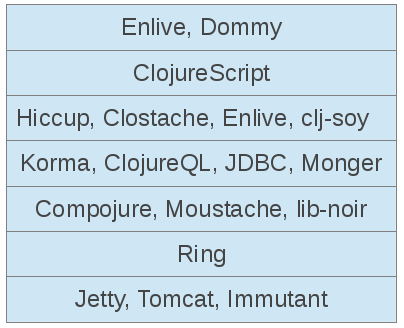
\includegraphics[height=4cm]{119_2013_w_figure1}
\caption{Библиотеки Сlojure для различных модулей архитектуры веб"=приложения}\label{fig:Bushenko1}
\end{figure}


\begin{figure}[h]
  \centering
  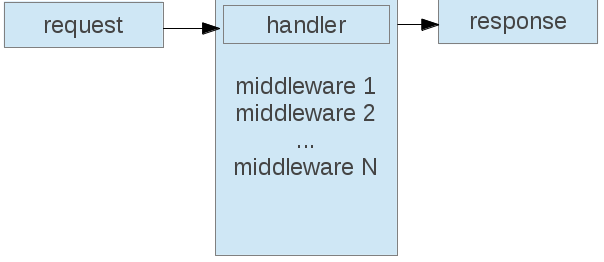
\includegraphics[height=3cm]{119_2013_w_figure2}
\caption{Ring}\label{fig:Bushenko2}
\end{figure}


Уровень маршрутизатора реализуют библиотеки Ring, \linebreak Compojure и Moustache.

Ring "--- это практически голый сервлет, каким он был бы, если бы его написали в функциональном стиле \cite{Bushenko3}. Центральная абстракция этой библиотеки "--- handler, который обрабатывает request и создает response (рис. \ref{fig:Bushenko2}). И request, и response "--- это обычные структуры данных Clojure "--- отображения. Композиция из функций"=middleware и handler"=ов задают бизнес"=логику обработки запроса. Как видите, это строгий функциональный подход.



Mustache и Compojure "--- это небольшие надстройки над Ring, каждый из которых по"=своему упрощает отображение маршрутов на функции, их обрабатывающие.

Уровень доступа к данным представлен несколькими интересными библиотеками, наиболее заметные из которых "--- это Korma и ClojureQL.
Korma "--- это библиотека, декларирующая, что она все"=таки не ORM \cite{Bushenko4}. Учитывая функциональную природу программ на Clojure, Object"=Relational Mapping"=у здесь и впрямь взяться неоткуда. Результаты запросов к БД представлены в виде векторов и отображений, а сами запросы записываются на удобном предметно"=ориентированном языке, внешне сильно напоминающем SQL.

ClojureQL схожа с Korma в том, что это предметно"=ориентированный язык \cite{Bushenko5}. Но, в отличие от Korma, семантика ClojureQL ближе к чистой реляционной алгебре, нежели к SQL.

Уровень представления реализуется целым рядом библиотек, соответствующих современным тенденциям. Hiccup "--- это то, как выглядел бы Haml, если бы его изначально написали на Clojure \cite{Bushenko6}. Clostache "--- это порт Mustache на Clojure, а clj"=soy "--- порт Google Closure Templates. Особенного внимания заслуживает библиотека Enlive, аналогов которой по сути и нету \cite{Bushenko7}. Она сильно напоминает XSLT т.к. занимается преобразованием исходного html"=файла по заданным правилам. Но, в отличие от XSLT, у которого громоздкий, неудобный синтаксис, Enlive делает все кратко и элегантно.
Важной частью инфраструктуры программ на Clojure является ClojureScript "--- реализация Clojure, компилирующегося в JavaScript \cite{Bushenko8}. Для ClojureScript также существует несколько шаблонизаторов, самые заметные из которых "--- Dommy \cite{Bushenko9} и Enfocus \cite{Bushenko10} (порт Hiccup и Enlive на ClojureScript). Использование Clojure на всех уровнях, начиная от доступа к БД, заканчивая UI"=логикой, позволяет отказаться от целого ряда лишних действий. Например, нет нужды генерировать ORM"=привязки к таблицам БД, очень упрощается передача данных с сервера на клиент, отпадает необходимость во всех промежуточных протоколах вроде SOAP или JSON.

Применение Clojure в web"=разработке позволяет также использовать всю гибкость Lisp"=а для построения предметно"=ориентированных языков. На примере библиотек доступа к данным мы видели, насколько удобно бывает разработать маленький, сфокусированный на определенном типе задач язык и решать задачи именно на нем. Clojure позволяет создавать такие языки с минимальными усилиями.

Таким образом, язык Clojure очень хорошо подходит для разработки web"=приложений. Он обладает отличной инфраструктурой, бесшовно интегрируется с любым java"=кодом и может деплоиться на стандартных серверах приложений java. Гибкость языка Clojure и его потрясающая выразительность позволяют создавать web"=приложения за минимальное время.

\begin{thebibliography}{99}

\bibitem{Bushenko1} Clojure, \url{http://clojure.org}
\bibitem{Bushenko2} Clojure Toolbox, \url{http://www.clojure-toolbox.com}
\bibitem{Bushenko3} Ring, \url{https://github.com/ring-clojure/ring}
\bibitem{Bushenko4} Korma, \url{http://sqlkorma.com}
\bibitem{Bushenko5} ClojureQL, \url{http://www.clojureql.org}
\bibitem{Bushenko6} Hiccup, \url{https://github.com/weavejester/hiccup}
\bibitem{Bushenko7} Enlive, \url{https://github.com/cgrand/enlive}
\bibitem{Bushenko8} ClojureScript, \url{https://github.com/clojure/clojurescript}
\bibitem{Bushenko9} Dommy, \url{https://github.com/Prismatic/dommy}
\bibitem{Bushenko10} Enfocus, \url{http://ckirkendall.github.com/enfocus-site}
\end{thebibliography}

\end{document}





\documentclass[10pt, a5paper]{article}
\usepackage{pdfpages}
\usepackage{parallel}
\usepackage[T2A]{fontenc}
\usepackage{ucs}
\usepackage[utf8x]{inputenc}
\usepackage[polish,english,russian]{babel}
\usepackage{hyperref}
\usepackage{rotating}
\usepackage[inner=2cm,top=1.8cm,outer=2cm,bottom=2.3cm,nohead]{geometry}
\usepackage{listings}
\usepackage{graphicx}
\usepackage{wrapfig}
\usepackage{longtable}
\usepackage{indentfirst}
\usepackage{array}
\newcolumntype{P}[1]{>{\raggedright\arraybackslash}p{#1}}
\frenchspacing
\usepackage{fixltx2e} %text sub- and superscripts
\usepackage{icomma} % коскі ў матэматычным рэжыме
\PreloadUnicodePage{4}

\newcommand{\longpage}{\enlargethispage{\baselineskip}}
\newcommand{\shortpage}{\enlargethispage{-\baselineskip}}

\def\switchlang#1{\expandafter\csname switchlang#1\endcsname}
\def\switchlangbe{
\let\saverefname=\refname%
\def\refname{Літаратура}%
\def\figurename{Іл.}%
}
\def\switchlangen{
\let\saverefname=\refname%
\def\refname{References}%
\def\figurename{Fig.}%
}
\def\switchlangru{
\let\saverefname=\refname%
\let\savefigurename=\figurename%
\def\refname{Литература}%
\def\figurename{Рис.}%
}

\hyphenation{admi-ni-stra-tive}
\hyphenation{ex-pe-ri-ence}
\hyphenation{fle-xi-bi-li-ty}
\hyphenation{Py-thon}
\hyphenation{ma-the-ma-ti-cal}
\hyphenation{re-ported}
\hyphenation{imp-le-menta-tions}
\hyphenation{pro-vides}
\hyphenation{en-gi-neering}
\hyphenation{com-pa-ti-bi-li-ty}
\hyphenation{im-pos-sible}
\hyphenation{desk-top}
\hyphenation{elec-tro-nic}
\hyphenation{com-pa-ny}
\hyphenation{de-ve-lop-ment}
\hyphenation{de-ve-loping}
\hyphenation{de-ve-lop}
\hyphenation{da-ta-ba-se}
\hyphenation{plat-forms}
\hyphenation{or-ga-ni-za-tion}
\hyphenation{pro-gramming}
\hyphenation{in-stru-ments}
\hyphenation{Li-nux}
\hyphenation{sour-ce}
\hyphenation{en-vi-ron-ment}
\hyphenation{Te-le-pathy}
\hyphenation{Li-nux-ov-ka}
\hyphenation{Open-BSD}
\hyphenation{Free-BSD}
\hyphenation{men-ti-on-ed}
\hyphenation{app-li-ca-tion}

\def\progref!#1!{\texttt{#1}}
\renewcommand{\arraystretch}{2} %Іначай формулы ў матрыцы зліпаюцца з лініямі
\usepackage{array}

\def\interview #1 (#2), #3, #4, #5\par{

\section[#1, #3, #4]{#1 -- #3, #4}
\def\qname{LVEE}
\def\aname{#1}
\def\q ##1\par{{\noindent \bf \qname: ##1 }\par}
\def\a{{\noindent \bf \aname: } \def\qname{L}\def\aname{#2}}
}

\def\interview* #1 (#2), #3, #4, #5\par{

\section*{#1\\{\small\rm #3, #4. #5}}

\def\qname{LVEE}
\def\aname{#1}
\def\q ##1\par{{\noindent \bf \qname: ##1 }\par}
\def\a{{\noindent \bf \aname: } \def\qname{L}\def\aname{#2}}
}


\begin{document}

\title{Ускорение загрузки Linux на ARM"=процессоре}%\footnote{Текст данных и последующих тезисов, кроме специально оговоренных случаев, доступен под лицензией Creative Commons Attribution-ShareAlike 3.0}

\author{Андрей Пушкин\footnote{Минск, Беларусь; \url{andrew.pushkin@gmail.com}}}
\maketitle

\begin{abstract}
Speeding up Linux loading on ARM SOC is considered. Steps to speed up loading Linux on ARM board: review boot scheme (initramfs, no initramfs, filesystems, user space soft) and check loading time of all booting parts; customize pre"=bootloader (on ARM TI AM3517 CPU is X"=Load), turn off any console output, customize memory timings; customize bootloader (U"=Boot), turn off any unused peripheral, rewrite some slow places; customize Linux kernel, turn off all unused options, move everything else to modules that come later; customize user space soft, loading GUI prior to other soft.
\end{abstract}

Перед автором была поставлена задача максимально ускорить процесс загрузки устройства с embedded Linux. Был предложен следующий план работы:

\begin{enumerate}
  \item Изучение работы системы и разбиениее ее на отдельные части для последующей оптимизации.
  \item Измерение времени загрузки каждого компонента системы. Для измерения использовались вывод отладочных сообщений в UART с засеканием времени их появления на Host"=PC.
  \item Оптимизация времени загрузки каждого компонента.
  \item Измерение времени работы оптимизированной системы, фиксация результатов.
Изначальное время загрузки устройства составляло 48 секунд. Исходным требованием было сократить время загрузки минимум до 5 секунд.
\end{enumerate}

Устройство имело следующую конфигурацию:

\begin{enumerate}
  \item Процессор Texas Instruments AM3505 (600 Mhz Cortex"=A8)
  \item 128 MB LPDDR2 RAM
  \item 256 MB NAND
  \item Touchscreen $320\times240$
  \item USB Host, USB Device, MMC, Bluetooth
\end{enumerate}

В начале работы система была разбита на модули и было измерено время загрузки каждого из них. Данные оказались следующими:

\begin{enumerate}
  \item X"=Load	- 200 миллисекунд
  \item U"=Boot	- 15050 миллисекунд
  \item Linux	- 9200 миллисекунд
  \item User Space Soft "--- 22000 миллисекунд
\end{enumerate}

\textbf{X"=Load "--- предварительный загрузчик}

В момент разработки проекта был актуален, сейчас x"=load интегрирован в U"=Boot и называется SPL.
Из X"=Load было вырезано всё, что связано с отладочным UART. Это дало выигрыш в 150 миллисекунд.

\textbf{U"=Boot "--- загрузчик ядра операционной системы}

В U"=Boot были сделаны следующие оптимизации:

\begin{enumerate}
  \item Изменение алгоритма загрузки
  -- Отказ от Initramfs. Суть Initramfs заключается что что Linux + rootfs читаются из NAND одним образом.
  -- Возврат к классической схеме загрузки, когда u"=boot читает только маленький образ ядра операционной системы без rootfs"=программ.
  Это дало выигрыш в 7300 миллисекунд.
  \item Отказ от подсчёта CRC в образе ядра Linux (в файле uImage). По"=умолчанию U"=boot считает контрольную сумму, и если она не совпадает с тем, что записано в uImage "--- не загружает его. Отказ от этой схемы привел к тому, что u"=boot всегда загружает ядро Linux, и дал выигрыш в 1200 миллисекунд.
  \item Уменьшение размера ядра Linux путём вынесения всего, что можно, в модули, которые загружаются позже. Это позволило уменьшить ядро Linux и значительно ускорить его чтение. Выигрыш составил 600 миллисекунд.
  \item Включение аппаратного NAND ECC дало выигрыш в 200 миллисекунд.
  \item Удаление инициализации из U"=Boot неиспользуемых частей: I²C, SPI, USB Host, USB device, MMC, драйверов ext2"=3, VFAT дало выигрыш в 700 миллисекунд.
  \item Встраивание картинки «Loading» (чтобы показать, что прибор загружается) в образ U"=boot взамен считывания ее картинки с NAND"=памяти дало выигрыш в 100 миллисекунд.
  \item Переписывание memmove под Cortex"=A8. Это дало выигрыш в 2250 миллисекунд
Всё в сумме привело к времени загрузки в 3000 миллисекунд вместо 15050.
\end{enumerate}

\textbf{Оптимизация Linux}

Были сделаны следующие оптимизации:

\begin{enumerate}
  \item Удаление из конфига ядра инициализации всего «лишнего» (ненужные драйвера, отладочные опции и так далее). Это дало выигрыш в 100 миллисекунд
  \item Вынесение всего, что возможно, в модули, которые загружаются позже. Это дало выигрыш в 8150 миллисекунд.
Всё в сумме дало время загрузки в 1050 миллисекунд вместо 9200.
\end{enumerate}

\textbf{Оптимизация User Space}

Схема загрузки до оптимизации включала следующие этапы:

\begin{enumerate}
  \item Ядро Linux
  \item Init скрипты
  \item Монтирование раздела с настройками
  \item Монтирование раздела с данными
  \item Запуск Qt4 GUI программы.
\end{enumerate}

В ходе оптимизации был убран раздел с настройками, которые стали хранится на основном разделе. Графическая программа на Qt4 начала запускаться как можно раньше чтобы показать меню программы как можно раньше, а остальные части загружать позднее.

В результате получилась следующая схема загрузки:

\begin{enumerate}
  \item Ядро Linux
  \item Qt4 GUI (не блокирующий запуск)
  \item Init скрипты
  \item Загрузка модулей ядра Linux
  \item Монтирование раздела с данными
  \item запуск Qt4 GUI программы
\end{enumerate}

Также в ходе оптимизации было сделано следующее:

\begin{enumerate}
  \item Перед запуском графической Qt4"=программы ставится её скриношот. Сама программа запускается 1500 миллисекунд.
  \item Файловая система заменена с JFFS2 на UBI, что дало выигрыш 5--10 секунд на монтировании
  \item Графическая Qt4"=программа переписана таким образом, чтобы сначала загружались те её части, которые отвечают за главное меню, и лишь потом "--- всё остальное
\end{enumerate}

В ходе работы были получены результаты:

\begin{enumerate}
  \item Показ меню прибора за 5 секунд
  \item Показ графического ПО за 6.5 секунд
  \item Полная загрузка прибора за 27 секунд
\end{enumerate}


\end{document}





\documentclass[10pt, a5paper]{article}
\usepackage{pdfpages}
\usepackage{parallel}
\usepackage[T2A]{fontenc}
\usepackage{ucs}
\usepackage[utf8x]{inputenc}
\usepackage[polish,english,russian]{babel}
\usepackage{hyperref}
\usepackage{rotating}
\usepackage[inner=2cm,top=1.8cm,outer=2cm,bottom=2.3cm,nohead]{geometry}
\usepackage{listings}
\usepackage{graphicx}
\usepackage{wrapfig}
\usepackage{longtable}
\usepackage{indentfirst}
\usepackage{array}
\newcolumntype{P}[1]{>{\raggedright\arraybackslash}p{#1}}
\frenchspacing
\usepackage{fixltx2e} %text sub- and superscripts
\usepackage{icomma} % коскі ў матэматычным рэжыме
\PreloadUnicodePage{4}

\newcommand{\longpage}{\enlargethispage{\baselineskip}}
\newcommand{\shortpage}{\enlargethispage{-\baselineskip}}

\def\switchlang#1{\expandafter\csname switchlang#1\endcsname}
\def\switchlangbe{
\let\saverefname=\refname%
\def\refname{Літаратура}%
\def\figurename{Іл.}%
}
\def\switchlangen{
\let\saverefname=\refname%
\def\refname{References}%
\def\figurename{Fig.}%
}
\def\switchlangru{
\let\saverefname=\refname%
\let\savefigurename=\figurename%
\def\refname{Литература}%
\def\figurename{Рис.}%
}

\hyphenation{admi-ni-stra-tive}
\hyphenation{ex-pe-ri-ence}
\hyphenation{fle-xi-bi-li-ty}
\hyphenation{Py-thon}
\hyphenation{ma-the-ma-ti-cal}
\hyphenation{re-ported}
\hyphenation{imp-le-menta-tions}
\hyphenation{pro-vides}
\hyphenation{en-gi-neering}
\hyphenation{com-pa-ti-bi-li-ty}
\hyphenation{im-pos-sible}
\hyphenation{desk-top}
\hyphenation{elec-tro-nic}
\hyphenation{com-pa-ny}
\hyphenation{de-ve-lop-ment}
\hyphenation{de-ve-loping}
\hyphenation{de-ve-lop}
\hyphenation{da-ta-ba-se}
\hyphenation{plat-forms}
\hyphenation{or-ga-ni-za-tion}
\hyphenation{pro-gramming}
\hyphenation{in-stru-ments}
\hyphenation{Li-nux}
\hyphenation{sour-ce}
\hyphenation{en-vi-ron-ment}
\hyphenation{Te-le-pathy}
\hyphenation{Li-nux-ov-ka}
\hyphenation{Open-BSD}
\hyphenation{Free-BSD}
\hyphenation{men-ti-on-ed}
\hyphenation{app-li-ca-tion}

\def\progref!#1!{\texttt{#1}}
\renewcommand{\arraystretch}{2} %Іначай формулы ў матрыцы зліпаюцца з лініямі
\usepackage{array}

\def\interview #1 (#2), #3, #4, #5\par{

\section[#1, #3, #4]{#1 -- #3, #4}
\def\qname{LVEE}
\def\aname{#1}
\def\q ##1\par{{\noindent \bf \qname: ##1 }\par}
\def\a{{\noindent \bf \aname: } \def\qname{L}\def\aname{#2}}
}

\def\interview* #1 (#2), #3, #4, #5\par{

\section*{#1\\{\small\rm #3, #4. #5}}

\def\qname{LVEE}
\def\aname{#1}
\def\q ##1\par{{\noindent \bf \qname: ##1 }\par}
\def\a{{\noindent \bf \aname: } \def\qname{L}\def\aname{#2}}
}


\begin{document}

\title{Поддержка шины TDM в ядре Linux}%\footnote{Текст данных и последующих тезисов, кроме специально оговоренных случаев, доступен под лицензией Creative Commons Attribution-ShareAlike 3.0}

\author{Михаил Курочкин, Александр Городинский\footnote{Минск, Беларусь; \url{stelhs@ya.ru}, \url{testor@zazoid.com}}}
\maketitle

\begin{abstract}
Because of the lack of support for TDM bus in the Linux kernel we decided to implement such driver and commit it the mainline. This thesis describes the TDM technology, its scope, and some of the nuances of implementation. Also it describes the possible prospects of its development, and development of the VoIP on Linux in general.
\end{abstract}

\subsection*{Telepathy}

Поводом для написания данного тезиса послужила наша работа по реализации
поддержки стандарта TDM в ядре Linux. Мы хотим рассказать вам об этом
стандарте, о том, почему мы решили реализовать его поддержку и какие это
открывает перспективы для других разработчиков и рядовых пользователей
ядра Linux.

Вообще говоря, TDM "--- это не совсем стандарт, это скорее принцип,
подразумевающий временное разделение информационного пространства канала.
TDM расшифровывается как Time Division \linebreak Multiplexing, что следует понимать
примерно как мультиплексирование посредством разделения во времени. Все
просто: ряд устройств висят на одной шине и каждое из них ждет своей
очереди для отправки данных. В отличие от некоторых других реализаций
общей шины, эти устройства никогда не пытаются и в принципе не могут
пытаться передать свои данные одновременно, потому что у каждого
устройства есть свой так называемый time slot, и каждое конкретное
устройство может принимать или передавать данные только в пределах данного
тайм"=слота, то есть некого промежутка времени.

Кроме тайм"=слота, в рамках данной концепции существует более общая
временная велечина назывемая кадром или фрэймом. Фрэйм "--- это то, что
объединяет все тайм"=слоты, т.е. за период в один фрэйм все устройства
зарегистрированные на шине имеют свои промежутки времени для обмена
данными, и принцип TDM гарантирует, что в каждый конкретный момент вермени
только одно устройство имеет право работать с шиной.

Фрэймы и тайм"=слоты отсчитываются при помощи специальных сигналов, которые
обычно передаются по специально выделенным для этого физическим линиям. За
формирование этих сигналов отвечает контроллер шины, которым обычно
является одно из устройств висящих на шине, хотя в принципе это не
обязательно.

Что это означает на практике? На практике данный подход имеет свои
преимущества и конечно же недостатки. Преимущества, это в первую очередь
соответствие требованиям realtime, то есть данная шина обеспечивает
нулевую задержку и стопроцентную гарантию передачи данных, даже в том
случае, если одновременно с этой шиной работают все имеющиеся в наличии
устройства. Достигается это за счет того, что тактовая частота TDM шины
оказывается достаточной для передачи данных генерируемых всеми
устройствами, которые на ней находятся. В случае если речь идет о
аудио"=устройствах "--- это не представляет никакой проблемы, поскольку объем
генерируемых ими данных очень невелик.

Недостатком TDM как принципа передачи данных является то, что если
какие"=то устройства неактивны в течение нескольких кадров, то устройства
которые выполняют передачу данных в этот момент не могут использовать
освободившиеся тайм"=слоты. Таким образом, если активны не все устройства,
то физический канал передачи данных используется лишь частично.

Однако следует понимать, что данная шина обычно используется для
реализации аудио"=подсистемы некого устройства, а в этом случае необходимо
гарантировать возможность одновременной работы всех компонентов системы,
т.е. всех устройств на шине. Как раз в этом случае, концепция TDM является
не только приемлемой, но даже оптимальной, поскольку она полностью
исключает оверхэд на обработку коллизий и гарантирует, что пропускная
способность канала передачи данных в принципе не может быть превышена. То
есть это значит, что все устройства будут работать одновременно и
стабильно, что и требуется.

Вообще говоря, стандарт TDM очень старый и возможно тем, кто был знаком с
ним раньше покажется странным, что его реализация внезапно появляется во
вполне современных устройствах, а его поддержка находится на стадии
аппрува перед добавлением его в ядро Linux. По"=видимому, это как раз тот
случай, когда некий стандарт или концепция прижившись в одной сфере,
оказывается более чем востребованной уровнем ниже. Когда"=то очень давно, в
80"=х годах двадцатого века, TDM нашел широкое применение для соединения
телефонных станций между собой, а теперь тот же принцип используется для
соединение динамика и микрофона с процессором мобильного телефона.
Забавно, правда? На самом деле, подобных примеров очень много, но к
сожалению, объем статьи не позволяет мне рассказать даже о самых
примечательных из них.

С другой стороны, в каком"=то смысле, поддержка TDM существует в ядре Linux
довольно давно, но никогда прежде никто не пытался вынести поддержку этой
концепции в отдельный фрэймворк, по аналогии с тем, как это сделано для
других шин и стандартов. Теперь же, когда данная реализация пройдет все
необходимые проверки и будет добавлена в код ядра, у других разработчиков
появиться прекрасная возможность не изобретать велосипед каждый раз при
написании драйвера для своего устройства, а использовать API
предоставляемый TDM фрэймворком.

Данный фрэймворк позволяет абстрагировать взаимодействие с шиной TDM и
привести это взаимодействие к некому единому стандарту, лишь по мере
необходимости добавляя поддержку конкретных контроллеров, а так же прочих
устройств, которые могут быть к данной шине подключены. То есть
использование данной реализации, является практикой повторного
использования кода, которая является одним из базовых механизмов
экосистемы OpenSource.

Что бы внести немного конкретики, приведу такую аналогию: отдаленного это
напоминает подсистему работы с последовательными портами. Так вот, наш TDM
"--- это как поддержка последовательного порта в прицнипе, в то время как для
работы с конкретной реализацией TDM требуется поддержка соответствующего
оборудования, примерно как для реальной работы с UART требуется поддержка
конкретной микросхемы.

Продолжая аналогию, считаю необходимым отметить, что шина TDM, точно так
же как и последовательная шина, никоим образом не регламентирует тайминги,
напряжения, назначение линий и прочее, все это определяется конкретной
реализацией от конкретного производителя. Тем не менее, реализация
универсального фрэймворка на уровне ядра, позволяет нам унифицировать
взаимодействие с устройствами висящими на данной шине, по аналогии с тем,
как это сделано в случае последовательного порта.

Говоря о существующих стандартах, было бы уместно привести примеры того,
как именно данная концепция используется в реально существующих
устройствах. А используется она очень широко: преимущественно это
устройства ориентированные на работу со звуком или содержащие работу со
звуком в своем функционале. Как правило, применение данного стандарта
особенно оправданно там, где нужно работать с большим количеством
относительно медленных сигналов, т.е. идеальным примером является звуковая
карта с большим количеством входов и выходов. Использование TDM позволяет
обойтись одной единственной шиной даже для весьма внушительного кличества
входов и выходов. И это не голая теория, в реальности очень многие
звуковые карты действительно содержат в своем устройстве такого рода шину.
Еще одним, не менее уместным применением данной шины являются DAQ boards,
т.е. платы захвата аналоговых данных, содержащие большое или даже огромное
количество входов. Данные платы являются узкоспециализированными и как
правило проприетарными устройствами, поэтому нам мало известно о том, как
именно они устроены, но если сигналы ими отрабатываемые слишком быстрые
для расширения количества входов простым мультиплексированием, то шина TDM
может быть одинм из самых оптимальных решений.

Ну и конечно нам хотелось бы рассказать о нашем устройстве, в работе
которого так же участвует шина TDM. Данное устройство относится к классу
CPE, что расшифровывается как Costumer Premise Equipment. На деле эта
формулировка означает, что часть функционала, который мог бы располагаться
на стороне провайдера, ATC или оператора кабельного телевидения, может
быть перенесена на сторону абонента, причем со значительной выгодой как
для для абонента, так и для всех перечисленных поставщиков услуг. Выгода
это выражается в совокупном удешевлении оборудования, в упрощении
принципов доставки контента и конечно же в расширении доступного
пользователю функционала. Одним из ключевых компонентов данного
функционала является конечно же телефония, а точнее "--- IP"=телефония. В
качестве основы для реализации VoIP подсистемы мы выбрали широко
распространенное, стабильное и функционально развитое решение "--- PBX
Asterisk. Наша система построена на базе Linux"=дистрибутива OperWRT,
поэтому в плане интеграции в программную платформу никаких проблем не
возникло "--- asterisk есть в репозитории данного дистрибутива.

А вот с поддержкой наших аппаратных средств возникли определенные
трудности. В качестве аппаратной платформы наша система использует SoC
Marvell Kirkwood, в составе которого есть ряд подсистем, драйверы для
которых реализованы исключительно в рамках поставляемого с данным чипом
SDK. Часть драйверов нам удалось перенести из данной SDK в инфарструктуру
OpenWRT и это было вполне оправданно, однако поддержка существующего на
чипе TDM на тот момент отсутствовала даже в составе SDK, не говоря уже про
mainline kernel. В свете этих фактов нами было принято решение начать
разработку собственного драйвера. В процессе работы над драйвером
выяснилось, что в новой версии SDK внезапно появилась поддержка данного
функционала, причем поддерживалась не только сама шина TDM, но и SLIC,
который был уже установлен на нашу плату и висел на этой шине. SLIC, это
subscriber line interface card, т.е. в сущности то самое аудио"=устройство
использующее шину TDM "--- еще один удачный пример из жизни, где TDM
оказывается полезным.

Таким образом, мы стали перед выбором, использовать предлагаемый
поставщиком драйвер, или заканчивать работу над собственным. В итоге было
принято решение завершить работу над нашим драйвером, в результате чего мы
сейчас имеем предмет для написания данной статьи, а сообщество имеет живой
и работающий пример того, как должно выглядеть повторное использование
кода и разделение уровней абстракции в процессе реализации поддержки
сложных аппаратных систем.

Выглядит это примерно так: TDM фрэймворк обеспечивает поддержку некой
абстракции, а в рамках этой абстракции поддерживается конкретная
реализация TDM от Marvell и микросхема SLIC. Данное решение прекрасно
работает в нашем устройстве, а при желании можно без особых проблем
добавить поддержку любых других реализаций TDM и любых устройств,
совместимых с этой шиной.

Существование нашего фрэйморка в mainline kernel может существенно ускорить
дальнейшее развитие IP"=телефонии на платформе Linux, а также даст нам
много других существенных бонусов, в виде более быстрой и качественной
разработки новых драйверов для звуковых карт, гарнитур, плат захвата
данных и многих других устройств, в которых используется эта простая,
надежная и крайне эффективная шина.


\end{document}





\documentclass[10pt, a5paper]{article}
\usepackage{pdfpages}
\usepackage{parallel}
\usepackage[T2A]{fontenc}
\usepackage{ucs}
\usepackage[utf8x]{inputenc}
\usepackage[polish,english,russian]{babel}
\usepackage{hyperref}
\usepackage{rotating}
\usepackage[inner=2cm,top=1.8cm,outer=2cm,bottom=2.3cm,nohead]{geometry}
\usepackage{listings}
\usepackage{graphicx}
\usepackage{wrapfig}
\usepackage{longtable}
\usepackage{indentfirst}
\usepackage{array}
\newcolumntype{P}[1]{>{\raggedright\arraybackslash}p{#1}}
\frenchspacing
\usepackage{fixltx2e} %text sub- and superscripts
\usepackage{icomma} % коскі ў матэматычным рэжыме
\PreloadUnicodePage{4}

\newcommand{\longpage}{\enlargethispage{\baselineskip}}
\newcommand{\shortpage}{\enlargethispage{-\baselineskip}}

\def\switchlang#1{\expandafter\csname switchlang#1\endcsname}
\def\switchlangbe{
\let\saverefname=\refname%
\def\refname{Літаратура}%
\def\figurename{Іл.}%
}
\def\switchlangen{
\let\saverefname=\refname%
\def\refname{References}%
\def\figurename{Fig.}%
}
\def\switchlangru{
\let\saverefname=\refname%
\let\savefigurename=\figurename%
\def\refname{Литература}%
\def\figurename{Рис.}%
}

\hyphenation{admi-ni-stra-tive}
\hyphenation{ex-pe-ri-ence}
\hyphenation{fle-xi-bi-li-ty}
\hyphenation{Py-thon}
\hyphenation{ma-the-ma-ti-cal}
\hyphenation{re-ported}
\hyphenation{imp-le-menta-tions}
\hyphenation{pro-vides}
\hyphenation{en-gi-neering}
\hyphenation{com-pa-ti-bi-li-ty}
\hyphenation{im-pos-sible}
\hyphenation{desk-top}
\hyphenation{elec-tro-nic}
\hyphenation{com-pa-ny}
\hyphenation{de-ve-lop-ment}
\hyphenation{de-ve-loping}
\hyphenation{de-ve-lop}
\hyphenation{da-ta-ba-se}
\hyphenation{plat-forms}
\hyphenation{or-ga-ni-za-tion}
\hyphenation{pro-gramming}
\hyphenation{in-stru-ments}
\hyphenation{Li-nux}
\hyphenation{sour-ce}
\hyphenation{en-vi-ron-ment}
\hyphenation{Te-le-pathy}
\hyphenation{Li-nux-ov-ka}
\hyphenation{Open-BSD}
\hyphenation{Free-BSD}
\hyphenation{men-ti-on-ed}
\hyphenation{app-li-ca-tion}

\def\progref!#1!{\texttt{#1}}
\renewcommand{\arraystretch}{2} %Іначай формулы ў матрыцы зліпаюцца з лініямі
\usepackage{array}

\def\interview #1 (#2), #3, #4, #5\par{

\section[#1, #3, #4]{#1 -- #3, #4}
\def\qname{LVEE}
\def\aname{#1}
\def\q ##1\par{{\noindent \bf \qname: ##1 }\par}
\def\a{{\noindent \bf \aname: } \def\qname{L}\def\aname{#2}}
}

\def\interview* #1 (#2), #3, #4, #5\par{

\section*{#1\\{\small\rm #3, #4. #5}}

\def\qname{LVEE}
\def\aname{#1}
\def\q ##1\par{{\noindent \bf \qname: ##1 }\par}
\def\a{{\noindent \bf \aname: } \def\qname{L}\def\aname{#2}}
}

\begin{document}
\title{Introduction to distributed file systems. OrangeFS experience}
\author{Andrew Savchenko\footnote{Moscow, Russia; NRNU MEPhI; \url{bircoph@gmail.com}}}
\maketitle
\begin{abstract}
An introduction to the world of distributed file systems is presen\-ted with a humble attempt to categorize them. A problem of choice is
considered from the workload profile point of view, and some common issues and pitfalls are discussed. A practical OrangeFS experience is
given with tips and tricks for better performance.
\end{abstract}
\section*{Preface}

Why one needs a non-local file system? Goals may vary, but usually they arise from the need of:

\begin{itemize}
  \item a \emph{large} data storage;
  \item a \emph{high performance} data storage;
  \item \emph{redundant} and highly available solutions.
\end{itemize}

There are dozens of solutions available\cite{bib1}, and many of them are open source. But how to choose one you need? There is a lot of ambiguity and vagueness in this field, but let's try to sort it out.

Focusing on open source solutions, one can see they are usually sufficient for any needs and are used on the most high performance systems from Top-500\cite{bib2} list, especially in the top 50 of them.

\section*{Species of distributed file systems}

Even the term ``distributed'' is ambiguous itself. It may mean all kinds of file systems running on more than a single host (sense used in a title of this article), but it also means a subset of this common sense discussed below. It should be understandable, that there is no canonical definitions in this field, so terminology found in different sources may vary.

Every non-local file system (except for few exotic cases) may be roughly related to one of the following classes:

\begin{itemize}
  \item network file systems;
  \item clustered file systems;
  \item distributed file systems.
\end{itemize}

Of course, there is a large intersection between these sets. See fig. \ref{fig:Sav1} for details.

\begin{figure}[h]
  \centering
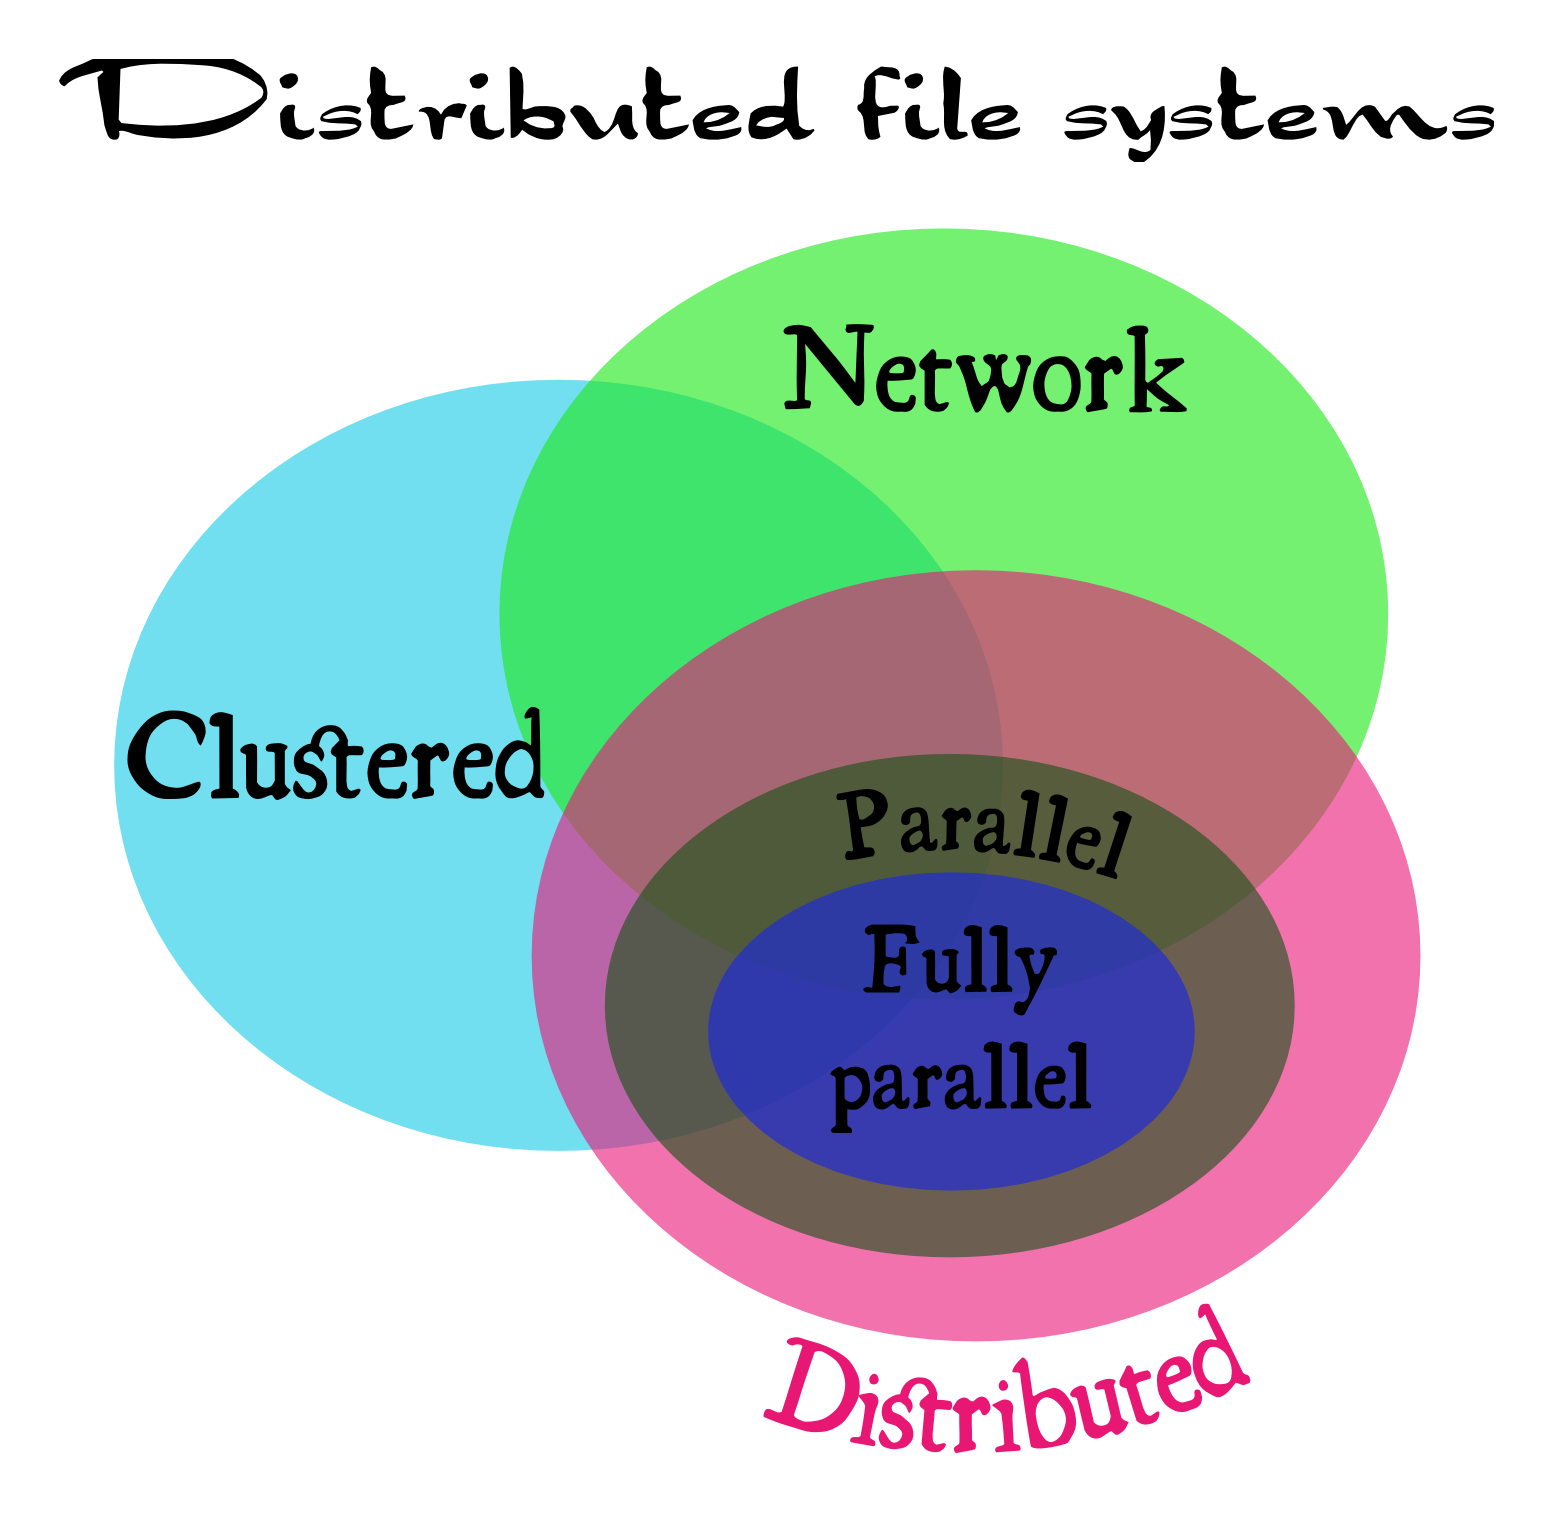
\includegraphics[height=4cm]{123_genesis.png}
\caption{Distributed flesystems}\label{fig:Sav1}
\end{figure}

\subsection*{Network file systems}

Network file system usually means one with a single server (or at least an appearance of a single server) and several remotely connected clients. Classical NFS\cite{bib3} is a good example (but not with pNFS\cite{bib4} extension).

\subsection*{Clustered file systems}

Clustered file system is a file system simultaneously mounted on several local servers sharing the same data storage on a block level (usually the SAN\cite{bib5} model is used). These kind of setups is called \emph{shared disk} file systems often. Well known examples are OCFS2\cite{bib6} and GFS2\cite{bib7} file systems.

\subsection*{Distributed file systems}

Distributed (in a narrow sense) file systems are setups with multiple data servers sharing nothing between them, for each active server its own data storage is private to it. This systems usually are not geographi\-cally distributed and are local in their location due to demands of high performance interconnect (e.g. pNFS\cite{bib3} extension of NFS\cite{bib2} falls here). But there are solutions present for geographically distributed systems, even for setups distributed across different continents. Andrew File System (AFS\cite{bib8}) is a good and widely used example.

\subsection*{Parallel file systems}

Whenever file system is called parallel, this means it provides a parallel access to (usually all of) its storage hosts for each of its clients. This allows to avoid a bottleneck of a single host in terms of both network and I/O bandwidth, latency; CPU and cache limitations. These file systems are usually used in the High Performance Computing \linebreak (HPC\cite{bib2}\cite{bib9}) and high-end business applications like stock exchange information systems. Prominent open source examples are Lustre\cite{bib10}, OrangeFS\cite{bib11} and Ceph\cite{bib12}.

\subsubsection*{Fully parallel file systems}

Parallel file systems are fully parallel when not only data, but meta\-data are also distributed on multiple servers and are accessible in parallel by clients. This is quite important for high-end performance as single metadata server will eventually become a bottleneck, especially when dealing with large directories. For example, OrangeFS\cite{bib11} and Ceph\cite{bib12} are fully parallel distributed file systems, but pNFS\cite{bib4} ad Lustre\cite{bib10} are not.

\subsection*{Highly Available (HA) solutions}

Each class described above may contain an HA solution. Usually this is done by either a data replication (as in Ceph\cite{bib12}) or by a disk level redundancy (RAID5/6) together with a server level redundancy (heartbeat/pacemaker) as in Lustre\cite{bib10} or OrangeFS\cite{bib11}.

\subsection*{MPI support}

If you're working in the HPC\cite{bib9} field, you'll be definitely interested in the MPI\cite{bib13} I/O support. ROMIO\cite{bib14} implements just that and is supported by many file systems, e.g. NFS\cite{bib3}, Lustre\cite{bib10}, OrangeFS\cite{bib11}.

\section*{Setup considerations}

Final choise should be made based on targeted applications for your setup:

\begin{itemize}
  \item is POSIX compliance setup required? Especially POSIX file locking, it hinders greatly distributed file system performance (and is not available on many file systems at all), but may be required by some applications;
  \item is MPI\cite{bib13} needed?
  \item is HA needed?
  \item what kind of locality are you targeted on?
  \item are your data servers exclusive for your storage tasks?
  \item are you working in trusted environment?
  \item and many more\ldots{}
\end{itemize}

\emph{Optimize} your software:

\begin{itemize}
  \item prefer a small number of large files over a large number of small files, as large directories hinder metadata servers greatly;
  \item prefer large data chunks over a large number of small network packets — they hinder TCP/IP stack greatly.
\end{itemize}

\section*{OrangeFS experience}

At our university we selected OrangeFS because of the following:

\begin{itemize}
  \item parallel distributed FS with good MPI support;
  \item reasonable performance on large directories;
  \item optional HA support;
  \item low CPU load;
  \item high network I/O performance (limited only by physical 1 Gbit/s bandwidth);
  \item native InfiniBand\cite{bib15} support.
\end{itemize}

Though, high performance means non full POSIX compliance, so:

\begin{itemize}
  \item no hardlinks;
  \item no special files;
  \item no unlink(): if file is gone, then it is gone immediately and forever.
  \item OrangeFS should not be used for \$HOME.
\end{itemize}

Setup hints:

\begin{itemize}
  \item use as many data \emph{and} metadata servers as possible;
  \item use large stip\_size, 1 MB is a good idea to start with;
  \item TroveSync may be disabled to improve speed at the cost of possible data loss when server dies;
  \item on ethernet use jumbo frames.
\end{itemize}

This software is a good example of how ordinary user sends patches made due to daily needs and became a project contributor :)

\section*{Summary}

There is no perfect distributed filesystem: to achieve the best in one aspect some others must be sacrificed. But if you understand your workload, you'll be able to pick up a few solutions, study them to your best and have fun!

In my humble opinion the most interesting and promising solutions for their fields are: Lustre\cite{bib10}, OrangeFS\cite{bib11}, Ceph\cite{bib12} and pNFS\cite{bib4}.

P.S. Always send your patches!

\begin{thebibliography}{9}
\bibitem{bib1} {\href{http://en.wikipedia.org/wiki/List_of_file_systems}{http://en.wikipedia.org/wiki/List\_of\_file\_systems}}
\bibitem{bib2} {\href{http://www.top500.org/}{http://www.top500.org/}}
\bibitem{bib3} {\href{http://linux-nfs.org/}{http://linux-nfs.org/}}
\bibitem{bib4} {\href{http://www.pnfs.com/}{http://www.pnfs.com/}}
\bibitem{bib5} {\href{http://en.wikipedia.org/wiki/Storage_area_network}{http://en.wikipedia.org/wiki/Storage\_area\_network}}
\bibitem{bib6} {\href{https://oss.oracle.com/projects/ocfs2/}{https://oss.oracle.com/projects/ocfs2/}}
\bibitem{bib7} {\href{https://access.redhat.com/knowledge/docs/en-US/Red_Hat_Enterprise_Linux/6/html/Global_File_System_2/ch-overview-GFS2.html}{https://access.redhat.com/knowledge/docs/en-US/Red\_Hat\_Enterprise\_Linux/6/html/Global\_File\_System\_2/ch-overview-GFS2.html}}
\bibitem{bib8} {\href{http://www.openafs.org/}{http://www.openafs.org/}}
\bibitem{bib9} {\href{http://en.wikipedia.org/wiki/Supercomputer}{http://en.wikipedia.org/wiki/Supercomputer}}
\bibitem{bib10} {\href{http://lustre.org/}{http://lustre.org}}
\bibitem{bib11} {\href{http://www.orangefs.org/}{http://www.orangefs.org/}}
\bibitem{bib12} {\href{http://ceph.com/}{http://ceph.com/}}
\bibitem{bib13} {\href{http://en.wikipedia.org/wiki/Message_Passing_Interface}{http://en.wikipedia.org/wiki/Message\_Passing\_Interface}}
\bibitem{bib14} {\href{http://www.mcs.anl.gov/research/projects/romio/}{http://www.mcs.anl.gov/research/projects/romio/}}
\bibitem{bib15} {\href{http://en.wikipedia.org/wiki/InfiniBand}{http://en.wikipedia.org/wiki/InfiniBand}}\end{thebibliography}
\end{document}

\documentclass[10pt, a5paper]{article}
\usepackage{pdfpages}
\usepackage{parallel}
\usepackage[T2A]{fontenc}
\usepackage{ucs}
\usepackage[utf8x]{inputenc}
\usepackage[polish,english,russian]{babel}
\usepackage{hyperref}
\usepackage{rotating}
\usepackage[inner=2cm,top=1.8cm,outer=2cm,bottom=2.3cm,nohead]{geometry}
\usepackage{listings}
\usepackage{graphicx}
\usepackage{wrapfig}
\usepackage{longtable}
\usepackage{indentfirst}
\usepackage{array}
\newcolumntype{P}[1]{>{\raggedright\arraybackslash}p{#1}}
\frenchspacing
\usepackage{fixltx2e} %text sub- and superscripts
\usepackage{icomma} % коскі ў матэматычным рэжыме
\PreloadUnicodePage{4}

\newcommand{\longpage}{\enlargethispage{\baselineskip}}
\newcommand{\shortpage}{\enlargethispage{-\baselineskip}}

\def\switchlang#1{\expandafter\csname switchlang#1\endcsname}
\def\switchlangbe{
\let\saverefname=\refname%
\def\refname{Літаратура}%
\def\figurename{Іл.}%
}
\def\switchlangen{
\let\saverefname=\refname%
\def\refname{References}%
\def\figurename{Fig.}%
}
\def\switchlangru{
\let\saverefname=\refname%
\let\savefigurename=\figurename%
\def\refname{Литература}%
\def\figurename{Рис.}%
}

\hyphenation{admi-ni-stra-tive}
\hyphenation{ex-pe-ri-ence}
\hyphenation{fle-xi-bi-li-ty}
\hyphenation{Py-thon}
\hyphenation{ma-the-ma-ti-cal}
\hyphenation{re-ported}
\hyphenation{imp-le-menta-tions}
\hyphenation{pro-vides}
\hyphenation{en-gi-neering}
\hyphenation{com-pa-ti-bi-li-ty}
\hyphenation{im-pos-sible}
\hyphenation{desk-top}
\hyphenation{elec-tro-nic}
\hyphenation{com-pa-ny}
\hyphenation{de-ve-lop-ment}
\hyphenation{de-ve-loping}
\hyphenation{de-ve-lop}
\hyphenation{da-ta-ba-se}
\hyphenation{plat-forms}
\hyphenation{or-ga-ni-za-tion}
\hyphenation{pro-gramming}
\hyphenation{in-stru-ments}
\hyphenation{Li-nux}
\hyphenation{sour-ce}
\hyphenation{en-vi-ron-ment}
\hyphenation{Te-le-pathy}
\hyphenation{Li-nux-ov-ka}
\hyphenation{Open-BSD}
\hyphenation{Free-BSD}
\hyphenation{men-ti-on-ed}
\hyphenation{app-li-ca-tion}

\def\progref!#1!{\texttt{#1}}
\renewcommand{\arraystretch}{2} %Іначай формулы ў матрыцы зліпаюцца з лініямі
\usepackage{array}

\def\interview #1 (#2), #3, #4, #5\par{

\section[#1, #3, #4]{#1 -- #3, #4}
\def\qname{LVEE}
\def\aname{#1}
\def\q ##1\par{{\noindent \bf \qname: ##1 }\par}
\def\a{{\noindent \bf \aname: } \def\qname{L}\def\aname{#2}}
}

\def\interview* #1 (#2), #3, #4, #5\par{

\section*{#1\\{\small\rm #3, #4. #5}}

\def\qname{LVEE}
\def\aname{#1}
\def\q ##1\par{{\noindent \bf \qname: ##1 }\par}
\def\a{{\noindent \bf \aname: } \def\qname{L}\def\aname{#2}}
}

\begin{document}
\title{Luwrain — адаптированная ОС с речевым интерфейсом}
\author{Михаил Пожидаев \footnote{Томск, Россия, \url{msp@altlinux.ru}}}
\maketitle
\begin{abstract}
The report covers new design of operating system for blind and visual impaired persons offered by the Luwrain project. Suggested conception includes text-based user interface without GUI elements as well as a number of system services managed through D-Bus. New approach to user interface implies\linebreak implementation with Java virtual machine. The project is based on conclusions of ALT Linux Homeros distribution respecting all positive parts of its experience.
\end{abstract}
Наиболее распространённый подход к использованию персонального компьютера людьми с проблемами зрения заключается в установке так называемых экранных чтецов, которые в виде речи описывают каждое действие пользователя и связанные с ним изменения на экране. Использование мыши обычно невозможно, и все манипуляции выполняются только при помощи клавиатуры. Графический пользовательский интерфейс (GUI) ориентирован главным образом на взаимодействие при помощи мыши, и в такой ситуации применение клавиатуры приводит к существенному увеличению времени работы. Обычно при работе дома или в тихом офисе дополнительные затраты времени несущественны, но в шумной и напряжённой обстановке крупного аэропорта или конференции навигация по элементам GUI с использованием клавиатуры становится утомительной и некомфортной.

Функции экранных чтецов позволяют организовать доступ к огромному числу приложений, но для людей с проблемами зрения круг необходимых задач намного уже, поскольку в него не входят решения, связанные с обработкой растровой и векторной графики, визуальным проектированием, видеомонтажом и пр. Закон Парето, согласно которому 80\% потребностей пользователей удовлетворяется 20\% функций приложений, приобретает более выраженный вид, что делает большое количество ПО на традиционных компьютерах незрячих пользователей невостребованным.

Проект Luwrain, проходящий в настоящий момент фазу подготовки первых демонстрационных прототипов, занимается разработкой новой среды для незрячих и слабовидящих пользователей, ориентированной на представление всех рабочих объектов только в текстовом виде. Главное требование, которому должен удовлетворять продукт, — предельно высокая скорость работы, а также хороший уровень комфорта и удобства пользователя даже в шумном и многолюдном помещении.

Среда функционирует внутри виртуальной машины Java с задействованием доступных библиотек для решения конкретных прикладных задач (JavaMail для чтения почты, Rome для чтения новостей, Apache POI для работы с форматами офисных документов и т. д.). Экран разделяется на фрагменты, расположенные в виде тайлов, которые условно называются ``области''. Каждая область позволяет выводить некоторую текстовую информацию, отображая её моноширинным шрифтом. Размер шрифта и его цвет можно менять в зависимости от уровня зрения слабовидящего человека. Пользователь имеет возможность свободной навигации по каждой области с получением соответствующих голосовых оповещений аналогично тому, как он перемещается внутри текстового файла. Содержание и поведение каждой области зависит от типа решаемой задачи. Например, если требуется составить электронное сообщение, то на первой строке под специальным заголовком указывается получатель, строкой ниже — тема сообщения и далее текст. Как показывает опыт, большинство необходимых задач может быть пересмотрено в описанном виде. В качестве экспериментальной платформы выступает дистрибутив ALT Linux Homeros, предлагающий похожую концепцию на базе текстового редактора GNU Emacs, но из-за ограничений среды неспособного стать продуктом для массового пользователя.

Виртуальная машина Java должна функционировать в\linebreak GNU/Linux, которая обеспечивает все необходимые системные компоненты. Особенное внимание планируется уделить сервисам, доступ к которым осуществляется через системную шину D-Bus. Примером таких сервисов может служить Network Manager, обеспечивающий управление сетевыми интерфейсами, Udisks, обеспечивающий управление носителями информации и пр. Особенно перспективным выглядит задействование службы Systemd, которая находится в активной разработке. Все указанные сервисы, управляемые централизованно при помощи D-Bus, позволяют сделать среду целостной и интегрированной, предоставляя пользователю удобные инструменты взаимодействия со всеми компонентами. Программа установки может быть выполнена при помощи технологии клонирования LiveCD.

Некоторые сервисы предполагается реализовать отдельно вне виртуальной машины Java. К ним относятся речевой сервер и служба управления медиапроигрывателем. Речевой сервер получает команды на воспроизведение фрагментов текста и управляет вызовом речевых синтезаторов для  генерации звукового сигнала и посылки его в аудио-устройство в режиме реального времени. Назначение службы управления медиапроигрывателем очень близко к функциям привычного проигрывателя, но требуется добавление особого механизма закладок, нужных для чтения ``говорящих книг''. Помимо этого, существует специализированный формат книг для незрячих людей — Daisy, который также должен обслуживаться описанным сервисом.

Некоторые задачи не могут быть решены в рамках приведённой концепции. Это прежде всего справедливо для веб-браузера, природа которого не позволяет представлять содержимое страниц в текстовом виде, и для закрытых коммерческих приложений, таких как, например, Skype. Для их работы можно воспользоваться готовой службой AT-SPI, запуская приложения без какой-либо модификации, но внутри специального оконного менеджера, оснащённого речевыми оповещениями и управляемого при помощи комбинаций ``горячих'' клавиш.

\end{document}

\documentclass[10pt, a5paper]{article}
\usepackage{pdfpages}
\usepackage{parallel}
\usepackage[T2A]{fontenc}
\usepackage{ucs}
\usepackage[utf8x]{inputenc}
\usepackage[polish,english,russian]{babel}
\usepackage{hyperref}
\usepackage{rotating}
\usepackage[inner=2cm,top=1.8cm,outer=2cm,bottom=2.3cm,nohead]{geometry}
\usepackage{listings}
\usepackage{graphicx}
\usepackage{wrapfig}
\usepackage{longtable}
\usepackage{indentfirst}
\usepackage{array}
\newcolumntype{P}[1]{>{\raggedright\arraybackslash}p{#1}}
\frenchspacing
\usepackage{fixltx2e} %text sub- and superscripts
\usepackage{icomma} % коскі ў матэматычным рэжыме
\PreloadUnicodePage{4}

\newcommand{\longpage}{\enlargethispage{\baselineskip}}
\newcommand{\shortpage}{\enlargethispage{-\baselineskip}}

\def\switchlang#1{\expandafter\csname switchlang#1\endcsname}
\def\switchlangbe{
\let\saverefname=\refname%
\def\refname{Літаратура}%
\def\figurename{Іл.}%
}
\def\switchlangen{
\let\saverefname=\refname%
\def\refname{References}%
\def\figurename{Fig.}%
}
\def\switchlangru{
\let\saverefname=\refname%
\let\savefigurename=\figurename%
\def\refname{Литература}%
\def\figurename{Рис.}%
}

\hyphenation{admi-ni-stra-tive}
\hyphenation{ex-pe-ri-ence}
\hyphenation{fle-xi-bi-li-ty}
\hyphenation{Py-thon}
\hyphenation{ma-the-ma-ti-cal}
\hyphenation{re-ported}
\hyphenation{imp-le-menta-tions}
\hyphenation{pro-vides}
\hyphenation{en-gi-neering}
\hyphenation{com-pa-ti-bi-li-ty}
\hyphenation{im-pos-sible}
\hyphenation{desk-top}
\hyphenation{elec-tro-nic}
\hyphenation{com-pa-ny}
\hyphenation{de-ve-lop-ment}
\hyphenation{de-ve-loping}
\hyphenation{de-ve-lop}
\hyphenation{da-ta-ba-se}
\hyphenation{plat-forms}
\hyphenation{or-ga-ni-za-tion}
\hyphenation{pro-gramming}
\hyphenation{in-stru-ments}
\hyphenation{Li-nux}
\hyphenation{sour-ce}
\hyphenation{en-vi-ron-ment}
\hyphenation{Te-le-pathy}
\hyphenation{Li-nux-ov-ka}
\hyphenation{Open-BSD}
\hyphenation{Free-BSD}
\hyphenation{men-ti-on-ed}
\hyphenation{app-li-ca-tion}

\def\progref!#1!{\texttt{#1}}
\renewcommand{\arraystretch}{2} %Іначай формулы ў матрыцы зліпаюцца з лініямі
\usepackage{array}

\def\interview #1 (#2), #3, #4, #5\par{

\section[#1, #3, #4]{#1 -- #3, #4}
\def\qname{LVEE}
\def\aname{#1}
\def\q ##1\par{{\noindent \bf \qname: ##1 }\par}
\def\a{{\noindent \bf \aname: } \def\qname{L}\def\aname{#2}}
}

\def\interview* #1 (#2), #3, #4, #5\par{

\section*{#1\\{\small\rm #3, #4. #5}}

\def\qname{LVEE}
\def\aname{#1}
\def\q ##1\par{{\noindent \bf \qname: ##1 }\par}
\def\a{{\noindent \bf \aname: } \def\qname{L}\def\aname{#2}}
}

\begin{document}
\title{Выбор информационных систем. Продвижение открытые системы в Enterprise}
\author{Вячеслав Бочаров \footnote{Минск, Беларусь; \url{gazolin@tut.by}}}
\maketitle
\begin{abstract}
The report adresses some aspects of chosing information systems. Steps are proposed to examine, which should provide help to such communities as the LVEE and BSOFT to increase the market share of open source software in the enterprise segment.
\end{abstract}
\section*{Время альтернатив}

Время, когда какая-либо информационная система была востребована только в силу своей исключительности, уже прошло. 
Всегда имеется несколько альтернативных решений.

Любая компания, которая приняла решение о внедрении той или иной информационной системы, стоит перед выбором, обусловленным многими факторами. На него влияют компании-поставщики, интеграторы, собственные технические специалисты и консультанты.
Открытые информационные системы -- также участники данного рынка. Рассмотрим, какие преимущества они имеют, и какие шаги позволят продвигать open-source  к корпоративном сегменте.

\subsection*{Выбор информационной системы. Как это происходит}

Почему в современной инфраструктуре так мала доля открытого ПО в бизнес"=критичных приложениях, например СУБД, системах Unified Communication, почтовых системах, средствах виртуализации, и в тоже время уже пропорциональна в инфраструктурной системе?

Ответ прост: при выборе инфраструктуры, зарытой от бизнес"=пользователей, окончательное решение принимает технический специалист. Он руководствуется опытом таких же технических специалистов и во многом собственными предпочтениями.

При выборе бизнес"=критичных систем решение принимает владелец бизнес"=процесса, директор или сам владелец бизнеса, и опираться он будет на многочисленные факторы, среди которых предпочтение технических специалистов будет иметь, как показывает опыт, не решающее значение.

Какие же факторы учитываются в первую очередь?

\begin{enumerate}
  \item А -- экономический эффект от внедрения системы,
  \item В – риски, связанные с внедрением.
\end{enumerate}

При $A \textgreater{} B$  принимается решение о внедрении. При выборе из нескольких систем соответственно $[A1-B1]\textgreater{}[A2-B2]$ , чем больше тем больше эффективность и меньше риски, тем лучше.

Также не стоит забывать затраты на функционирование системы, так называемое TCO (Total cost of ownership) или стоимость владения информационной системой. В нее входят зарплаты, стоимость серверного и клиентского аппаратного обеспечения, стоимость внедрения и затраты на доработку, затраты на техническую поддержку.
Соответвенно, формула выбора выглядит как $[A1 - (TCO1 + B1)] \textgreater{} [A2-(TCO2 + B2)]$.

В эффективность входит прямая прибыль от внедрения, возможно, повышение выручки, снижение затрат, сокращение времени.
Перечисленное описывается термином ROI (Return on \linebreak Investment) или возврат от инвестиций.

Еще один показатель, влияющий на выбор информационной системы, это срок возврата от инвестиций (Pay-Back Period). Например, рассматриваемая информационная система окупается и начинает приносить прибыль в неприемлемо большие сроки, т.е. в ней заморожены инвестиции и активы.

В набор рисков входят:

\begin{enumerate}
  \item Риск того, что система не будет соответствовать полностью или частично заявленным требованиям.
  \item Риск того, что расчетные показатели TCO были недооценены, и затраты превышают ожидания.
  \item Риски того, что система не может модернизироваться, либо ее модернизация стоит неоправданно дорого.
  \item Законодательные риски, т.е. соответствие всех элементов системы законодательству.
\end{enumerate}

Как ни странно, не существует эффективной методики расчета рисков как таковой. При выборе информационные системы приходится оценивать по методу аналогии. Где, у кого такая информационная система внедрена? Каковы позиции на рынке у производителя информационной системы? Какой у интегратора есть опыт внедрения этой информационной системы, и кто может дать оценку успешности внедрения? Как планируется техническая поддержка информационной системы и ее развитие?
Немаловажно и мнение системного интегратора, имеющего в своем портфеле решений систему с открытым кодом.

Все сказанное дает представление о том, какие особенности приходится учитывать при выборе, помимо качества кода и полноты соответствия ТЗ.

\subsection*{Сравнение преимуществ и недостатков решений open source на рынке РБ}

Представим, что на основании сказанного нам, как бизнес"=пользователю,  предстоит выбрать систему.

\subsubsection*{Основные конкурентные преимущества Open-source:}

\begin{enumerate}
  \item Отсутствует плата за приобретение и использование.
  \item Открытый код может быть модернизирован и приспособлен к нуждам предприятия нашим собственным ИТ-подразделением либо привлеченными компаниями.
  \item Над совершенствованием кода работает сообщество независимых высокопрофессиональных специалистов, что позволяет своевременно выявлять и устранять ошибки и недостатки.
\end{enumerate}

\subsubsection*{Риски:}

\begin{enumerate}
  \item Отсутствие информации об успешных внедрениях информационной системы, либо ее недоступность для лиц, принимающих решение. Непрозрачность всех этапов внедрения.
  \item Отсутствие централизованной технической поддержки. Невозможность получить гарантированную договором поддержку информационной системы.
  \item Незаинтересованность системных интеграторов в предложениях открытых информационных систем, в виду отсутствия прибыли при их продаже.
  \item Устоявшиеся мифы о высоких затратах на оплату специалистов по поддержке Linux-систем, а также о небольшом количестве специалистов на рынке труда. Невозможность адекватно оценить уровень знаний специалистов.
\end{enumerate}

Несмотря на первоначальную привлекательность решения, риски также оказываются велики. Это и затраты на доработку / техническое обслуживание, и отсутствие интеграторов, и негарантированная техническая поддержка, и невозможность оценить опыт других внедрений.

\subsection*{Возможные действия}

В ситуации, когда сообщество пользователей открытых систем разрознено и не объединено, практически невозможно преодолеть опасения бизнес"=пользователей по использованию открытых систем.
Но в связи с развитием сообществ и общественных организаций, таких как LVEE и создаваемое Белорусское общество открытых технологий, появляется шанс переломить ситуацию.

По мнению автора, для этого необходимы следующие действия:

\begin{enumerate}
  \item Аккумулировать знания об успешных проектах по внедрению открытых систем, описывать и производить рассылку участникам сообщества и заинтересовавшимся бизнес"=пользователям, публиковать на тематических сайтах отчеты об успешных внедрениях, отзывы о достигнутых эффектах от внедрения. Это позволит оценить уровень сложности, затраты по внедрению.
  \item Более тесно взаимодействовать с системными интеграторами, предлагая новую схему получения прибыли на уровне сопровождения систем. Добиваться включения в их портфель решений на базе открытых систем. На данный момент системными интеграторами, например, такими как ``Белсофт'', высказана предварительная заинтересованность в открытых системах. Это поможет получить потенциальному пользователю уверенность в технической поддержке и сопровождении информационной системы.
  \item Совместно с государственными и коммерческими учебными центрами разработать программу оценки специалистов, проводить и публиковать анализ рынка труда по данным специальностям.
  \item При необходимости сообщества должны оказывать информационное сопровождение, услуги по консультированию проекта по внедрению.
\end{enumerate}

\end{document}

\documentclass[10pt, a5paper]{article}
\usepackage{pdfpages}
\usepackage{parallel}
\usepackage[T2A]{fontenc}
\usepackage{ucs}
\usepackage[utf8x]{inputenc}
\usepackage[polish,english,russian]{babel}
\usepackage{hyperref}
\usepackage{rotating}
\usepackage[inner=2cm,top=1.8cm,outer=2cm,bottom=2.3cm,nohead]{geometry}
\usepackage{listings}
\usepackage{graphicx}
\usepackage{wrapfig}
\usepackage{longtable}
\usepackage{indentfirst}
\usepackage{array}
\newcolumntype{P}[1]{>{\raggedright\arraybackslash}p{#1}}
\frenchspacing
\usepackage{fixltx2e} %text sub- and superscripts
\usepackage{icomma} % коскі ў матэматычным рэжыме
\PreloadUnicodePage{4}

\newcommand{\longpage}{\enlargethispage{\baselineskip}}
\newcommand{\shortpage}{\enlargethispage{-\baselineskip}}

\def\switchlang#1{\expandafter\csname switchlang#1\endcsname}
\def\switchlangbe{
\let\saverefname=\refname%
\def\refname{Літаратура}%
\def\figurename{Іл.}%
}
\def\switchlangen{
\let\saverefname=\refname%
\def\refname{References}%
\def\figurename{Fig.}%
}
\def\switchlangru{
\let\saverefname=\refname%
\let\savefigurename=\figurename%
\def\refname{Литература}%
\def\figurename{Рис.}%
}

\hyphenation{admi-ni-stra-tive}
\hyphenation{ex-pe-ri-ence}
\hyphenation{fle-xi-bi-li-ty}
\hyphenation{Py-thon}
\hyphenation{ma-the-ma-ti-cal}
\hyphenation{re-ported}
\hyphenation{imp-le-menta-tions}
\hyphenation{pro-vides}
\hyphenation{en-gi-neering}
\hyphenation{com-pa-ti-bi-li-ty}
\hyphenation{im-pos-sible}
\hyphenation{desk-top}
\hyphenation{elec-tro-nic}
\hyphenation{com-pa-ny}
\hyphenation{de-ve-lop-ment}
\hyphenation{de-ve-loping}
\hyphenation{de-ve-lop}
\hyphenation{da-ta-ba-se}
\hyphenation{plat-forms}
\hyphenation{or-ga-ni-za-tion}
\hyphenation{pro-gramming}
\hyphenation{in-stru-ments}
\hyphenation{Li-nux}
\hyphenation{sour-ce}
\hyphenation{en-vi-ron-ment}
\hyphenation{Te-le-pathy}
\hyphenation{Li-nux-ov-ka}
\hyphenation{Open-BSD}
\hyphenation{Free-BSD}
\hyphenation{men-ti-on-ed}
\hyphenation{app-li-ca-tion}

\def\progref!#1!{\texttt{#1}}
\renewcommand{\arraystretch}{2} %Іначай формулы ў матрыцы зліпаюцца з лініямі
\usepackage{array}

\def\interview #1 (#2), #3, #4, #5\par{

\section[#1, #3, #4]{#1 -- #3, #4}
\def\qname{LVEE}
\def\aname{#1}
\def\q ##1\par{{\noindent \bf \qname: ##1 }\par}
\def\a{{\noindent \bf \aname: } \def\qname{L}\def\aname{#2}}
}

\def\interview* #1 (#2), #3, #4, #5\par{

\section*{#1\\{\small\rm #3, #4. #5}}

\def\qname{LVEE}
\def\aname{#1}
\def\q ##1\par{{\noindent \bf \qname: ##1 }\par}
\def\a{{\noindent \bf \aname: } \def\qname{L}\def\aname{#2}}
}

\begin{document}
\title{Storm. Система распределенной обработки данных в реальном времени.}
\author{Andrei Piatrushenia \footnote{Minsk, Belarus}}
\maketitle
\begin{abstract}
Storm is a free and open source distributed realtime computation system. Storm makes it easy to reliably process unbounded streams of data, doing for realtime processing.
The report covers the most sufficient details of the Storm project, such as realtime stream processing, horizontal scalability, processing guarantee and fault-tolerance, installation, application deployment and some typical how-to's. 
Programming examples use Java.
\end{abstract}
Распределенные вычисления -- сегодняшняя объективная реальность. Технические и бизнес-задачи требоуют все больших вычислительных ресурсов. Как минимум последнее десятилетие большое распространение получили одноранговые гетерогенные системы на базе относительно простых вычислительных систем. Это всевозможные кластеры, облака и т.п.

Лидером прикладных систем распределенных вычислений, машинного обучения, статистического анализа, сбора данных и т.п. считается Apache Hadoop, впитавший в себя идеи BigData. Система успешно переросла детский возраст, имеет огромную сферу практического применения, накоплен опыт использования, реализации типовых задач.

Storm появился в рамках проекта BackType (приобретенного Twitter летом 2011), где был призван решить задачу, для которой Hadoop не подходил по главному критерию – сбор данных и их обработка должны были производиться в реальном времени, тогда как Hadoop предполагает их пакетную обработку. Конечно, такая задача могла быть решена и с помощью пакетной обработки, вызываемой по накоплении набора данных или через временные интервалы, но запросам главного инвестора такие «костыли» не отвечали.

В результате появился Storm, в основе которого лежит поточная обработка данных. 
В основе обработки данных лежат узлы распределенной сети (здесь и далее в контексте Storm – топологии) двух типов:
\begin{itemize}
\item Источники данных (Spout)
\item Обработчики данных (Bolt)
\end{itemize}

Первые – являются источниками данных. Они могут принимать их извне или генерировать. С точки зрения топологии источники данных входных данных не имеют.

Вторые служат для обработки, преобразования данных, сохранения, вывода и т.п.

Обработчики могут быть соединены в цепочки любой длины, делающие обработку данных потенциально бесконечной, возможна организация передачи данных от одного обработчика к другому на случайной основе, с реализацией регулировки нагрузки, сразу нескольким узлам и т.п.

Сам Storm отвечает за  организацию вычислительных узлов, передачу данных между ними, контроль доставки, уведомлений об обработке данных или отказе в ней, делая большую часть такой работы абсолютно прозрачной для программиста, реализующего каждый отдельный узел как «черный ящик» для остальных, декларируя при необходимости входные и выходные данные.

Построение вычислительного кластера Storm относительно простая задача, для каждого вычислительного узла необходимый минимум составляет: 
\begin{itemize}
\item JRE, storm реализован на closure и исполняется на виртуальной машине Java
\item Apache Zookeeper , для глобальной синхронизации между узлами
\item ZeroMQ  -- для синхронизации между процессами
\item Python – кусочек storm реализован на Python
\item Несколько минут на узел, если выполнять все действия вручную
\end{itemize}


Для удобства разработки Storm имеет локальный режим использования – для него нет необходимости организовывать вообще какое-либо окружение кроме бинарного дистрибутива Storm, все процессы выполняются на машине разработчика.

Основной сложностью для начинающего знакомиться со Storm является довольно минималистическая документация, скромное описание API (по сути – лишь декларирование), почти полное отсутствие off-line источников, первая книга по Storm покинула стены издательства осенью минувшего года.

Целью предстоящего доклада является раскрытие основных идей проекта Storm,  демонстрация основ организации топологий и вычислительных узлов на простых примерах, акцентирования принципиальных отличий Storm от других систем распределенной обработки данных.

Список литературы:

\begin{thebibliography}{9}
\bibitem{bib1} Сайт проекта \url{http://storm-project.net/}
\bibitem{bib2} Wiki \url{https://github.com/nathanmarz/storm/wiki}
\end{thebibliography}


\end{document}

%\documentclass[10pt, a5paper]{article}
\usepackage{pdfpages}
\usepackage{parallel}
\usepackage[T2A]{fontenc}
\usepackage{ucs}
\usepackage[utf8x]{inputenc}
\usepackage[polish,english,russian]{babel}
\usepackage{hyperref}
\usepackage{rotating}
\usepackage[inner=2cm,top=1.8cm,outer=2cm,bottom=2.3cm,nohead]{geometry}
\usepackage{listings}
\usepackage{graphicx}
\usepackage{wrapfig}
\usepackage{longtable}
\usepackage{indentfirst}
\usepackage{array}
\newcolumntype{P}[1]{>{\raggedright\arraybackslash}p{#1}}
\frenchspacing
\usepackage{fixltx2e} %text sub- and superscripts
\usepackage{icomma} % коскі ў матэматычным рэжыме
\PreloadUnicodePage{4}

\newcommand{\longpage}{\enlargethispage{\baselineskip}}
\newcommand{\shortpage}{\enlargethispage{-\baselineskip}}

\def\switchlang#1{\expandafter\csname switchlang#1\endcsname}
\def\switchlangbe{
\let\saverefname=\refname%
\def\refname{Літаратура}%
\def\figurename{Іл.}%
}
\def\switchlangen{
\let\saverefname=\refname%
\def\refname{References}%
\def\figurename{Fig.}%
}
\def\switchlangru{
\let\saverefname=\refname%
\let\savefigurename=\figurename%
\def\refname{Литература}%
\def\figurename{Рис.}%
}

\hyphenation{admi-ni-stra-tive}
\hyphenation{ex-pe-ri-ence}
\hyphenation{fle-xi-bi-li-ty}
\hyphenation{Py-thon}
\hyphenation{ma-the-ma-ti-cal}
\hyphenation{re-ported}
\hyphenation{imp-le-menta-tions}
\hyphenation{pro-vides}
\hyphenation{en-gi-neering}
\hyphenation{com-pa-ti-bi-li-ty}
\hyphenation{im-pos-sible}
\hyphenation{desk-top}
\hyphenation{elec-tro-nic}
\hyphenation{com-pa-ny}
\hyphenation{de-ve-lop-ment}
\hyphenation{de-ve-loping}
\hyphenation{de-ve-lop}
\hyphenation{da-ta-ba-se}
\hyphenation{plat-forms}
\hyphenation{or-ga-ni-za-tion}
\hyphenation{pro-gramming}
\hyphenation{in-stru-ments}
\hyphenation{Li-nux}
\hyphenation{sour-ce}
\hyphenation{en-vi-ron-ment}
\hyphenation{Te-le-pathy}
\hyphenation{Li-nux-ov-ka}
\hyphenation{Open-BSD}
\hyphenation{Free-BSD}
\hyphenation{men-ti-on-ed}
\hyphenation{app-li-ca-tion}

\def\progref!#1!{\texttt{#1}}
\renewcommand{\arraystretch}{2} %Іначай формулы ў матрыцы зліпаюцца з лініямі
\usepackage{array}

\def\interview #1 (#2), #3, #4, #5\par{

\section[#1, #3, #4]{#1 -- #3, #4}
\def\qname{LVEE}
\def\aname{#1}
\def\q ##1\par{{\noindent \bf \qname: ##1 }\par}
\def\a{{\noindent \bf \aname: } \def\qname{L}\def\aname{#2}}
}

\def\interview* #1 (#2), #3, #4, #5\par{

\section*{#1\\{\small\rm #3, #4. #5}}

\def\qname{LVEE}
\def\aname{#1}
\def\q ##1\par{{\noindent \bf \qname: ##1 }\par}
\def\a{{\noindent \bf \aname: } \def\qname{L}\def\aname{#2}}
}

\begin{document}
\title{Протокол IF-MAP}
\author{Олег Орел\footnote{Минск, Беларусь, EPAM Systems, \url{Aleh_Arol@epam.com}}}
\date{}
\maketitle
\begin{abstract}
The Interface for Metadata Access Points (IF-MAP) is an open standard client/server protocol developed as one of the core protocols of the Trusted Network Connect (TNC) open architec\-ture. IF-MAP provides a common interface between the database server acting as a clearinghouse for information about security events and objects, and other elements of the TNC architecture.
\end{abstract}

TNC (Trusted Network Connect) "--- архитектура, описывающая возможную реализацию подхода к сетевой компьютерной безопасности, унифицирующего решения по обеспечению безопасности на конечных узлах (такие как антивирусное ПО, системы обнаружения вторжений и т.~д.), пользовательскую аутентификацию, элементы обеспечения безопасности. Компьютер, подключившийся в сеть, получает уровень доступа к ресурсам по результатам анализа таких его параметров, как уровень защищенности от вредоносных программ, конфигурации, роли пользователя, обновлений ОС. По любому параметру доступ может быть разграничен: например, пользователь, чей компьютер не обладает свежими антивирусными базами, не будет допущен в Интернет. IF"=MAP "--- открытый стандарт, описывающий клиент"=серверный протокол обмена данных между элементами (MAP) в TNC"=архитектуре.
IF-MAP сервер "--- это централизованное хранилище метаданных (например, о состоянии узлов сети, пользователях и т.~д.), предоставляющее механизмы для публикации данных, поиска и подписок всем заинтересованным MAP"=клиентам. Модель данных, предусмотренная для IF-MAP сервиса, представляет собой граф, вершины которого "--- идентификаторы (device, ip-address, mac-address, access-request, \ldots), а ребра "--- метаданные. Например, метаданные типа ip-mac, которые публикует MAP"=клиент, работающий совместно с DHCP сервером, соединяют идентификаторы типа ip"=address и mac"=address (DHCP lease) и содержат дополнительную информацию (время действия адреса). MAP"=клиентам доступен поиск на этом графе, а система подписок на изменения позволяет выполнять отложенный поиск.


\end{document}



\documentclass[10pt, a5paper]{article}
\usepackage{pdfpages}
\usepackage{parallel}
\usepackage[T2A]{fontenc}
\usepackage{ucs}
\usepackage[utf8x]{inputenc}
\usepackage[polish,english,russian]{babel}
\usepackage{hyperref}
\usepackage{rotating}
\usepackage[inner=2cm,top=1.8cm,outer=2cm,bottom=2.3cm,nohead]{geometry}
\usepackage{listings}
\usepackage{graphicx}
\usepackage{wrapfig}
\usepackage{longtable}
\usepackage{indentfirst}
\usepackage{array}
\newcolumntype{P}[1]{>{\raggedright\arraybackslash}p{#1}}
\frenchspacing
\usepackage{fixltx2e} %text sub- and superscripts
\usepackage{icomma} % коскі ў матэматычным рэжыме
\PreloadUnicodePage{4}

\newcommand{\longpage}{\enlargethispage{\baselineskip}}
\newcommand{\shortpage}{\enlargethispage{-\baselineskip}}

\def\switchlang#1{\expandafter\csname switchlang#1\endcsname}
\def\switchlangbe{
\let\saverefname=\refname%
\def\refname{Літаратура}%
\def\figurename{Іл.}%
}
\def\switchlangen{
\let\saverefname=\refname%
\def\refname{References}%
\def\figurename{Fig.}%
}
\def\switchlangru{
\let\saverefname=\refname%
\let\savefigurename=\figurename%
\def\refname{Литература}%
\def\figurename{Рис.}%
}

\hyphenation{admi-ni-stra-tive}
\hyphenation{ex-pe-ri-ence}
\hyphenation{fle-xi-bi-li-ty}
\hyphenation{Py-thon}
\hyphenation{ma-the-ma-ti-cal}
\hyphenation{re-ported}
\hyphenation{imp-le-menta-tions}
\hyphenation{pro-vides}
\hyphenation{en-gi-neering}
\hyphenation{com-pa-ti-bi-li-ty}
\hyphenation{im-pos-sible}
\hyphenation{desk-top}
\hyphenation{elec-tro-nic}
\hyphenation{com-pa-ny}
\hyphenation{de-ve-lop-ment}
\hyphenation{de-ve-loping}
\hyphenation{de-ve-lop}
\hyphenation{da-ta-ba-se}
\hyphenation{plat-forms}
\hyphenation{or-ga-ni-za-tion}
\hyphenation{pro-gramming}
\hyphenation{in-stru-ments}
\hyphenation{Li-nux}
\hyphenation{sour-ce}
\hyphenation{en-vi-ron-ment}
\hyphenation{Te-le-pathy}
\hyphenation{Li-nux-ov-ka}
\hyphenation{Open-BSD}
\hyphenation{Free-BSD}
\hyphenation{men-ti-on-ed}
\hyphenation{app-li-ca-tion}

\def\progref!#1!{\texttt{#1}}
\renewcommand{\arraystretch}{2} %Іначай формулы ў матрыцы зліпаюцца з лініямі
\usepackage{array}

\def\interview #1 (#2), #3, #4, #5\par{

\section[#1, #3, #4]{#1 -- #3, #4}
\def\qname{LVEE}
\def\aname{#1}
\def\q ##1\par{{\noindent \bf \qname: ##1 }\par}
\def\a{{\noindent \bf \aname: } \def\qname{L}\def\aname{#2}}
}

\def\interview* #1 (#2), #3, #4, #5\par{

\section*{#1\\{\small\rm #3, #4. #5}}

\def\qname{LVEE}
\def\aname{#1}
\def\q ##1\par{{\noindent \bf \qname: ##1 }\par}
\def\a{{\noindent \bf \aname: } \def\qname{L}\def\aname{#2}}
}

\begin{document}
\title{Голос спонсора: SaM Solutions}
%\author{}
\date{}
\maketitle

Компания SaM Solutions выступает в роли системо-образующего спонсора конференции Linux Vacation Eastern Europe с момента рождения LVEE в 2005 году и на протяжении всех лет её проведения. 

Сложившаяся корпоративная практика не случайна. Продукты и решения, задействующие Linux и другие Free/Open Source Software проекты, составляют заметную часть пакета разработок SaM Solutions. Кадровая политика компании направлена на поощрение профессионального развития своих сотрудников, организацию их эффективного отдыха и привлечение хорошо мотивированных кандидатов к работе на компанию. Формат конференции LVEE успешно позволяет решать все три задачи. 

Одним из подразделений компании является отдел Linux и \linebreak Embbeded. Специалисты компании на протяжении десятилетий работают с СПО. Компанией реализован ряд проектов по адаптации ОС GNU/Linux для работы в различных устройствах, построенных на таких платформах как ARM, PowerPC, x86, MIPS. В последние годы "--- на ведущие позиции выходит разработка управляющего ПО для серверов Enterprise-класса, от низкоуровнего BMC Firmware на основе Linux до высокоуровневых систем контроля виртуализации и графических интерфейсов управления, от прошивок устройств хранения данных до BSP интегрированных плат для разработчика. Надёжность, качество и широкая функциональность множества свободных проектов позволяет строить нам системы любого уровня и сложности, опираясь на высококачественные готовые компоненты.

В рамках направления Linux и Embedded успешно выполнены проекты для таких знаковых заказчиков, как  Novell/SUSE, Fujitsu Technology Solutions  и осуществляется партнёрство с компаниями IBM и Oracle/Sun в области Open Source решений.

Мы разрабатываем, модифицируем и адаптируем различное свободное программное обеспечение для наших заказчиков, но не забываем и о своих нуждах "--- наши сотрудники используют в своей работе существующие програмные продукты и вносят вклад в их развитие. Часть внутренней инфраструктуры, а именно интранет-сеть компании, тестовые стенды отдела контроля качества, рабочие места сотрудников профильных подразделений "--- также работает под управлением СПО (серверные и десктопные платформы GNU/Linux и FreeBSD). 

В минувшем году, в рамках реорганизации, был разработан долгосрочный план развития направления Linux и Embedded в SaM Solutions. В нём впервые были кодифицированы уже имеющиеся внутренние неофициальные практики по взаимодействию с commu"=nity-based проектами. В частности разработаны меры и правила по
\begin{itemize}
  \item возврата изменений в родительские проекты (upstreaming);
  \item вхождения в состав постоянных разработчиков активно используемых нами FOSS-компонентов;
  \item публикации сообщений об ошибках (bug reporting);
  \item участия и помощи в организации community events;
  \item стимуляции докладов и участия в технических конференциях.
\end{itemize}
И план немедленно начал претворяться в жизнь.

Силами отдела организовано внутреннее обучение сотрудников на регулярной
основе. Был прочтен и опубликован курс по TDD. По согласованию с автором
опубликован курс Debian/Ubuntu Packaging (видео, презентация и исходные
тексты презентации в \LaTeX).  Были организованы и проведены курсы по
обучению QA специалистов для направления Embeded Linux. Проведено
практическое занятие по основам виртуализации и эмуляции, организована
лекция по вопросу профилирования и оптимизации Ruby-кода, лекция о
High-availability кластерах и направлении развития технологии. Кроме того,
проводился семинар по Video4Linux2. Для создания и обучения кадрового
резерва на ближайшее будущее запланированы постоянно действующие внутренние
проекты в области Embedded Linux, результаты которых также запланированы к
публикации.

Визиты представительных делегаций на Embedded World 2012 и Linux Con Europe/Embedded LinuxCon Europe 2011 обогатили нас новыми идеями, куда можно
двигаться дальше и что сейчас актуально. А выступления на Software
Engineering Forum for Students, круглом столе по СПО в рамках TIBO-2012
и LVEE Winter 2012 позволили поделиться опытом с
заинтересованными сторонами.

В апреле состоялась Ганноверская промышленная ярмарка \linebreak (Hannover Messe
2013). Компания SaM Solutions была представлена отдельным стендом, на
котором демонстрировались наработки в области встроенного и системного ПО
на базе OS Linux. Идея «умного» дома вызвала неподдельный интерес у
посетителей стенда.

При поддержке SaM Solutions, с декабря 2011 года возобновились регулярные встречи Minsk Linux Users Groups, под названием <<Линуксовка в SaM Solutions>>. Техническое оснащение линуксовок и открытый формат встреч позволил им практически мгновенно стать заметным дискуссионным клубом по широкому спектру вопросов, прямо или косвенно связанных с СПО. Свободная картография (OpenStreetMap), технологии виртуализации, минский \linebreak hackerspace, Linux Mobile, бойкот Голливудской продукции, systemd, загрузчик u-boot, белорусская локализация GNOME --- это только часть тем, поднятых за последние линуксовки.

Быстрые и положительные изменения, как внутри компании SaM Solutions, так и в экосфере СПО (и Linux в частности) наполняют нас уверенностью, что направление движения выбрано верно.

\begin{figure}[h!]
\centering
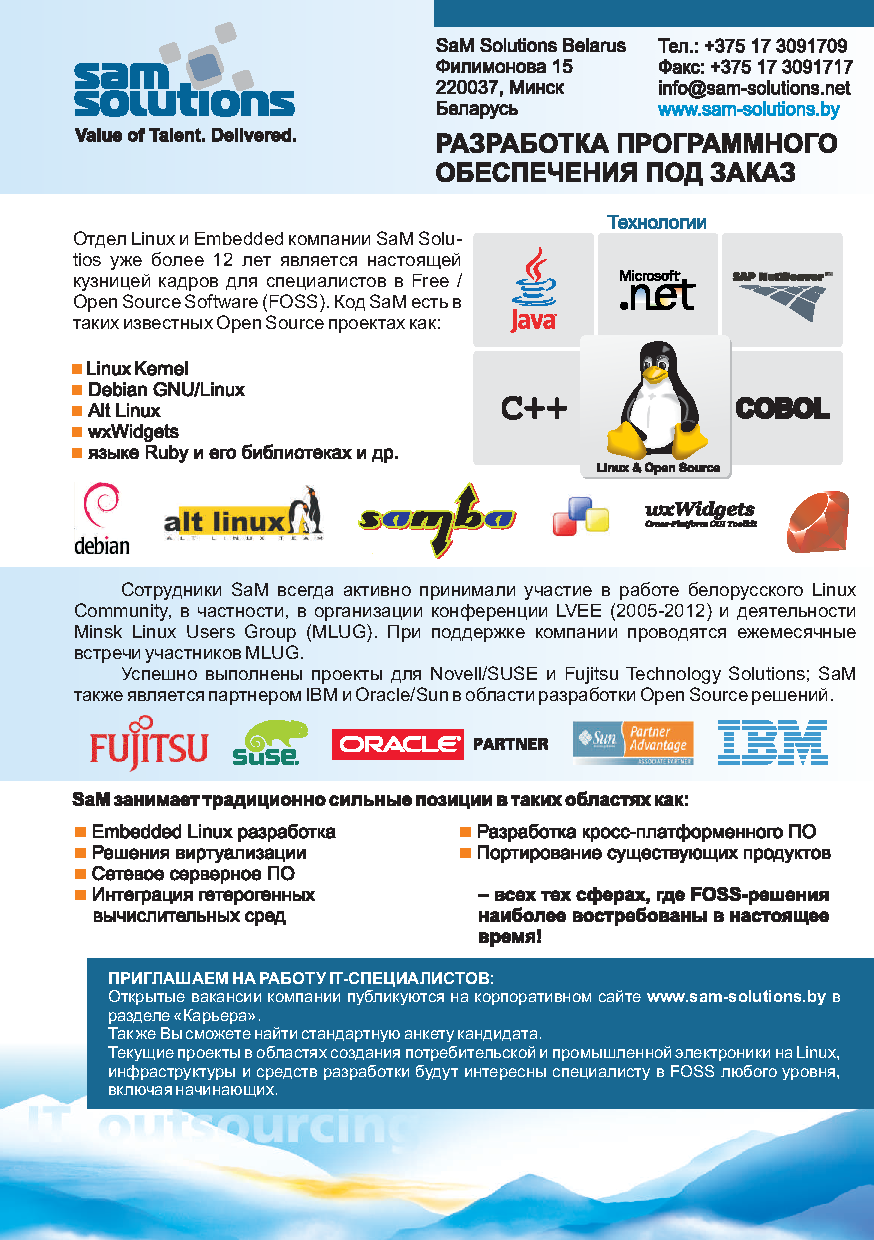
\includegraphics[height=11.8cm]{48_spons_sams.pdf}
\end{figure}
\end{document}



\documentclass[10pt, a5paper]{article}
\usepackage{pdfpages}
\usepackage{parallel}
\usepackage[T2A]{fontenc}
\usepackage{ucs}
\usepackage[utf8x]{inputenc}
\usepackage[polish,english,russian]{babel}
\usepackage{hyperref}
\usepackage{rotating}
\usepackage[inner=2cm,top=1.8cm,outer=2cm,bottom=2.3cm,nohead]{geometry}
\usepackage{listings}
\usepackage{graphicx}
\usepackage{wrapfig}
\usepackage{longtable}
\usepackage{indentfirst}
\usepackage{array}
\newcolumntype{P}[1]{>{\raggedright\arraybackslash}p{#1}}
\frenchspacing
\usepackage{fixltx2e} %text sub- and superscripts
\usepackage{icomma} % коскі ў матэматычным рэжыме
\PreloadUnicodePage{4}

\newcommand{\longpage}{\enlargethispage{\baselineskip}}
\newcommand{\shortpage}{\enlargethispage{-\baselineskip}}

\def\switchlang#1{\expandafter\csname switchlang#1\endcsname}
\def\switchlangbe{
\let\saverefname=\refname%
\def\refname{Літаратура}%
\def\figurename{Іл.}%
}
\def\switchlangen{
\let\saverefname=\refname%
\def\refname{References}%
\def\figurename{Fig.}%
}
\def\switchlangru{
\let\saverefname=\refname%
\let\savefigurename=\figurename%
\def\refname{Литература}%
\def\figurename{Рис.}%
}

\hyphenation{admi-ni-stra-tive}
\hyphenation{ex-pe-ri-ence}
\hyphenation{fle-xi-bi-li-ty}
\hyphenation{Py-thon}
\hyphenation{ma-the-ma-ti-cal}
\hyphenation{re-ported}
\hyphenation{imp-le-menta-tions}
\hyphenation{pro-vides}
\hyphenation{en-gi-neering}
\hyphenation{com-pa-ti-bi-li-ty}
\hyphenation{im-pos-sible}
\hyphenation{desk-top}
\hyphenation{elec-tro-nic}
\hyphenation{com-pa-ny}
\hyphenation{de-ve-lop-ment}
\hyphenation{de-ve-loping}
\hyphenation{de-ve-lop}
\hyphenation{da-ta-ba-se}
\hyphenation{plat-forms}
\hyphenation{or-ga-ni-za-tion}
\hyphenation{pro-gramming}
\hyphenation{in-stru-ments}
\hyphenation{Li-nux}
\hyphenation{sour-ce}
\hyphenation{en-vi-ron-ment}
\hyphenation{Te-le-pathy}
\hyphenation{Li-nux-ov-ka}
\hyphenation{Open-BSD}
\hyphenation{Free-BSD}
\hyphenation{men-ti-on-ed}
\hyphenation{app-li-ca-tion}

\def\progref!#1!{\texttt{#1}}
\renewcommand{\arraystretch}{2} %Іначай формулы ў матрыцы зліпаюцца з лініямі
\usepackage{array}

\def\interview #1 (#2), #3, #4, #5\par{

\section[#1, #3, #4]{#1 -- #3, #4}
\def\qname{LVEE}
\def\aname{#1}
\def\q ##1\par{{\noindent \bf \qname: ##1 }\par}
\def\a{{\noindent \bf \aname: } \def\qname{L}\def\aname{#2}}
}

\def\interview* #1 (#2), #3, #4, #5\par{

\section*{#1\\{\small\rm #3, #4. #5}}

\def\qname{LVEE}
\def\aname{#1}
\def\q ##1\par{{\noindent \bf \qname: ##1 }\par}
\def\a{{\noindent \bf \aname: } \def\qname{L}\def\aname{#2}}
}

\begin{document}
\title{Голос спонсора: EPAM Systems}
%\author{}
\date{}
\maketitle

Компания EPAM Systems не первый год является спонсором международной конференции разработчиков и пользователей свободного программного обеспечения LVEE (Linux Vacation / Eastern Europe). Этот год также не стал исключением. Пожалуй, LVEE является самым значимым событием для русскоязычных разработчиков и тестировщиков Open Source. Каждое лето здесь встречаются начинающие специалисты и «ветераны»"=разработчики из десятка стран для обмена опытом и общения на профессиональные темы. Наши специалисты также активно участвуют в данной конференции: в качестве докладчиков и организаторов/волонтёров. Это уникальная в своём роде конференция, и именно поэтому EPAM Systems очередной раз принимает участие в LVEE в качестве спонсора.


EPAM Systems "--- одна из крупнейших компаний"=поставщиков\linebreak услуг в области разработки программного обеспечения и решений на территории СНГ и Центральной и Восточной Европы. Созданная в 1993 году, сегодня она имеет представительства в 12 странах мира, в штате работают более 9 тыс. сотрудников, из которых более 3 тыс. "--- в Беларуси. Рост компании обеспечивается за счет собственных обучающих программ и передаче опыта от больших специалистов до начинающих разработчиков. Компания EPAM Systems выполняет проекты более чем в 30 странах мира. Основные направления деятельности: разработка, тестирование, сопровождение и поддержка заказного программного обеспечения и бизнес"=приложений, а также ИТ"=консалтинг с учетом отраслевой специфики бизнеса.

Наша компания участвует в проектах с такими крупными, хорошо известными заказчиками как Google, Novell, Infoblox, Parallels, 10Gen и др., так и с небольшими, в том числе и с начинающими свой путь в софтверном бизнесе.


К примеру, для Infoblox была реализована связка между WebUI с BIND и DHCP. Для этого был разработан комплекс решений под управлением Shell и Python скриптов, а также механизм позволяющий вносить правки в BIND и DHCP на языке C. Также был разработан развернутый функционал, автоматизирующий инсталляцию новых устройств и их эксплуатацию, что позволяет значительно упростить управление данными. Встроенный Web"=интерфейс позволяет разворачивать, управлять сервисами DNS, DNSSEC, DHCP, IPAM, устанавливать новые версии ПО, архивировать и восстанавливать из архивов необходимые данные, восстанавливать их после аварии, проводить мониторинг сети и создавать отчеты без необходимости обращения к командной строке.


Еще одним решением, реализованным для компании Infoblox, являлся программный продукт, позволяющий контролировать сетевые изменения, таким образом, облегчая идентификацию трудноуловимых проблем конфигурации и соответствие требованиям. Вместо того чтобы просто регистрировать изменения, система использует внесенную информацию для проверки, анализа и автоматической обработки сетевых изменений. Благодаря инновационной, квалифицированной, глубокой технике логического анализа, программа изолирует проблемы исправности и конфигурации до того, как они могут вызвать более серьезные сбои.


Разработанная для анализа сложных сетей система изучает сеть, собирает ключевую информацию, применяет встроенную технику логического анализа и создает оценку исправности сети и список проблем, требующих принятие мер для улучшения качества работы сети.


Правильное использование свободного ПО в разработках сокращает и расходы на покупку лицензионных программ, и трудозатраты при создании коммерческого ПО. Немалую роль для достижения превосходного результата играет привлечение к разработке опытных специалистов. LVEE способствует появлению таких специалистов, развитию их навыков и расширению кругозора. Хотелось бы пожелать участникам конференции интересных проектов и максимум пользы от участия в LVEE.


\end{document}



\documentclass[10pt, a5paper]{article}
\usepackage{pdfpages}
\usepackage{parallel}
\usepackage[T2A]{fontenc}
\usepackage{ucs}
\usepackage[utf8x]{inputenc}
\usepackage[polish,english,russian]{babel}
\usepackage{hyperref}
\usepackage{rotating}
\usepackage[inner=2cm,top=1.8cm,outer=2cm,bottom=2.3cm,nohead]{geometry}
\usepackage{listings}
\usepackage{graphicx}
\usepackage{wrapfig}
\usepackage{longtable}
\usepackage{indentfirst}
\usepackage{array}
\newcolumntype{P}[1]{>{\raggedright\arraybackslash}p{#1}}
\frenchspacing
\usepackage{fixltx2e} %text sub- and superscripts
\usepackage{icomma} % коскі ў матэматычным рэжыме
\PreloadUnicodePage{4}

\newcommand{\longpage}{\enlargethispage{\baselineskip}}
\newcommand{\shortpage}{\enlargethispage{-\baselineskip}}

\def\switchlang#1{\expandafter\csname switchlang#1\endcsname}
\def\switchlangbe{
\let\saverefname=\refname%
\def\refname{Літаратура}%
\def\figurename{Іл.}%
}
\def\switchlangen{
\let\saverefname=\refname%
\def\refname{References}%
\def\figurename{Fig.}%
}
\def\switchlangru{
\let\saverefname=\refname%
\let\savefigurename=\figurename%
\def\refname{Литература}%
\def\figurename{Рис.}%
}

\hyphenation{admi-ni-stra-tive}
\hyphenation{ex-pe-ri-ence}
\hyphenation{fle-xi-bi-li-ty}
\hyphenation{Py-thon}
\hyphenation{ma-the-ma-ti-cal}
\hyphenation{re-ported}
\hyphenation{imp-le-menta-tions}
\hyphenation{pro-vides}
\hyphenation{en-gi-neering}
\hyphenation{com-pa-ti-bi-li-ty}
\hyphenation{im-pos-sible}
\hyphenation{desk-top}
\hyphenation{elec-tro-nic}
\hyphenation{com-pa-ny}
\hyphenation{de-ve-lop-ment}
\hyphenation{de-ve-loping}
\hyphenation{de-ve-lop}
\hyphenation{da-ta-ba-se}
\hyphenation{plat-forms}
\hyphenation{or-ga-ni-za-tion}
\hyphenation{pro-gramming}
\hyphenation{in-stru-ments}
\hyphenation{Li-nux}
\hyphenation{sour-ce}
\hyphenation{en-vi-ron-ment}
\hyphenation{Te-le-pathy}
\hyphenation{Li-nux-ov-ka}
\hyphenation{Open-BSD}
\hyphenation{Free-BSD}
\hyphenation{men-ti-on-ed}
\hyphenation{app-li-ca-tion}

\def\progref!#1!{\texttt{#1}}
\renewcommand{\arraystretch}{2} %Іначай формулы ў матрыцы зліпаюцца з лініямі
\usepackage{array}

\def\interview #1 (#2), #3, #4, #5\par{

\section[#1, #3, #4]{#1 -- #3, #4}
\def\qname{LVEE}
\def\aname{#1}
\def\q ##1\par{{\noindent \bf \qname: ##1 }\par}
\def\a{{\noindent \bf \aname: } \def\qname{L}\def\aname{#2}}
}

\def\interview* #1 (#2), #3, #4, #5\par{

\section*{#1\\{\small\rm #3, #4. #5}}

\def\qname{LVEE}
\def\aname{#1}
\def\q ##1\par{{\noindent \bf \qname: ##1 }\par}
\def\a{{\noindent \bf \aname: } \def\qname{L}\def\aname{#2}}
}

%\frenchspacing
\begin{document}
\title{Голос спонсора: ITS Partner}
%\author{}
\date{}
\maketitle%

~

\end{document}



\documentclass[10pt, a5paper]{article}
\usepackage{pdfpages}
\usepackage{parallel}
\usepackage[T2A]{fontenc}
\usepackage{ucs}
\usepackage[utf8x]{inputenc}
\usepackage[polish,english,russian]{babel}
\usepackage{hyperref}
\usepackage{rotating}
\usepackage[inner=2cm,top=1.8cm,outer=2cm,bottom=2.3cm,nohead]{geometry}
\usepackage{listings}
\usepackage{graphicx}
\usepackage{wrapfig}
\usepackage{longtable}
\usepackage{indentfirst}
\usepackage{array}
\newcolumntype{P}[1]{>{\raggedright\arraybackslash}p{#1}}
\frenchspacing
\usepackage{fixltx2e} %text sub- and superscripts
\usepackage{icomma} % коскі ў матэматычным рэжыме
\PreloadUnicodePage{4}

\newcommand{\longpage}{\enlargethispage{\baselineskip}}
\newcommand{\shortpage}{\enlargethispage{-\baselineskip}}

\def\switchlang#1{\expandafter\csname switchlang#1\endcsname}
\def\switchlangbe{
\let\saverefname=\refname%
\def\refname{Літаратура}%
\def\figurename{Іл.}%
}
\def\switchlangen{
\let\saverefname=\refname%
\def\refname{References}%
\def\figurename{Fig.}%
}
\def\switchlangru{
\let\saverefname=\refname%
\let\savefigurename=\figurename%
\def\refname{Литература}%
\def\figurename{Рис.}%
}

\hyphenation{admi-ni-stra-tive}
\hyphenation{ex-pe-ri-ence}
\hyphenation{fle-xi-bi-li-ty}
\hyphenation{Py-thon}
\hyphenation{ma-the-ma-ti-cal}
\hyphenation{re-ported}
\hyphenation{imp-le-menta-tions}
\hyphenation{pro-vides}
\hyphenation{en-gi-neering}
\hyphenation{com-pa-ti-bi-li-ty}
\hyphenation{im-pos-sible}
\hyphenation{desk-top}
\hyphenation{elec-tro-nic}
\hyphenation{com-pa-ny}
\hyphenation{de-ve-lop-ment}
\hyphenation{de-ve-loping}
\hyphenation{de-ve-lop}
\hyphenation{da-ta-ba-se}
\hyphenation{plat-forms}
\hyphenation{or-ga-ni-za-tion}
\hyphenation{pro-gramming}
\hyphenation{in-stru-ments}
\hyphenation{Li-nux}
\hyphenation{sour-ce}
\hyphenation{en-vi-ron-ment}
\hyphenation{Te-le-pathy}
\hyphenation{Li-nux-ov-ka}
\hyphenation{Open-BSD}
\hyphenation{Free-BSD}
\hyphenation{men-ti-on-ed}
\hyphenation{app-li-ca-tion}

\def\progref!#1!{\texttt{#1}}
\renewcommand{\arraystretch}{2} %Іначай формулы ў матрыцы зліпаюцца з лініямі
\usepackage{array}

\def\interview #1 (#2), #3, #4, #5\par{

\section[#1, #3, #4]{#1 -- #3, #4}
\def\qname{LVEE}
\def\aname{#1}
\def\q ##1\par{{\noindent \bf \qname: ##1 }\par}
\def\a{{\noindent \bf \aname: } \def\qname{L}\def\aname{#2}}
}

\def\interview* #1 (#2), #3, #4, #5\par{

\section*{#1\\{\small\rm #3, #4. #5}}

\def\qname{LVEE}
\def\aname{#1}
\def\q ##1\par{{\noindent \bf \qname: ##1 }\par}
\def\a{{\noindent \bf \aname: } \def\qname{L}\def\aname{#2}}
}

\begin{document}
\title{Голос спонсора: World of Tanks team}
%\author{}
\date{}
\maketitle

\subsection*{О проекте}

World of Tanks (Мир танков) "--- первый ММО проект ААА класса, созданный
белоруской командой. Разработчиками игра позиционируется как MMO"=экшн с
элементами ролевой игры, шутера и стратегии. Концепция <<World of Tanks>>
базируется на массовых командных танковых сражениях в режиме PvP. Онлайн
релиз русской версии игры состоялся 12 августа 2010 года, в марте 2011 года
состоялся <<китайский>> релиз, а в апреле 2011 года проект успешно вышел на
территории США и Европы.

Успех проекта World of Tanks можно оценить по целому ряду показателей:
количество активных игроков более 2 миллионов, рекордная цифра одновременной
игры "--- более 150.000 игроков на российском игровом кластере! В книгу
рекордов Гиннеса мы вошли 23 января 2011 года с показателем 91 311 игроков
он"=лайн. 

Дважды подряд в 2010 и 2011 году на Конференции Разработчиков Компьютерных
Игр (Москва) наш проект был признан Лучшей клиентской он"=лайн игрой (КРИ
2010) и Лучшей игрой (КРИ 2011).

В 2010 году по результатам международной выставки E3 (Лос"=Анжелес)
крупнейший ММО"=портал Massivly назвал наш проект New Concept 2010. В
настоящий момент определяются победители E3 2011. Мы сможем рассказать о
наших успехах уже при личной встрече на конференции LVEE 2011.

\subsection*{Подробности о проекте}

Игровые кластеры проекта находятся в дата"=центрах России, Германии, США и
Китая. Общее количество серверов в настоящий момент порядка 500, к концу
года мы планируем удвоить их количество.

Как игровые, так и прочие инфраструктурные сервера функционируют на базе
операционной системы CentOS.

Осенью 2010 года пики онлайна на российском игровом кластере достигали 30
тыс. В настоящий момент за счет высокотехнологичных решений наших
специалистов (включающих в себя оптимизацию сетевой инфраструктуры,
оптимизацию работы с базами данных, оптимизацию нашего серверного ПО) пик
он-лайна вырос до 150 тыс.

Высокая производительность достигается в т.~ч. за счет использования
free and open source software  как технологической основы для работы
серверной части самой масштабной ММО"=игры, а именно: CentOS,
MySQL, nginx, zabbix, nagios, cacti, python, django и т.~д.

\subsection*{О нас}

Над созданием проекта работает СООО <<Гейм Стрим>> "--- основной центр разработки
компании \url{Wargaming.net}. История компании "--- это 12"=летний опыт создания игр,
более 15 выпущенных проектов, среди которых <<Операция Багратион>>, а так же
<<Order of War>>, изданная Square Enix. В 2007 году мы объединились с минской
студией Arise. В 2010 из разработчика превратились в издателя "--- мы сами
осуществляем оперирование проекта World of Tanks. 

Наши награды на Конференции Разработчиков Компьютерных Игр (Москва): лучшая стратегическая игра КРИ"=2008 (проект <<Операция Багратион>>),
приз от прессы КРИ"=2009, лучшая компания"=разработчик КРИ"=2009 и КРИ"=2010, приз от индустрии КРИ 2011, приз зрительских симпатий КРИ 2011.

Сейчас в студии работает более 200 человек. Мы готовимся к запуску в
производство новых проектов и будем рады знакомству с талантливыми
специалистами. 

Нашим будущим сотрудникам мы предлагаем уникальную возможность работать над
онлайн"=проектами ААА класса, с применением передовых технологических
решений; реализовать себя, работая над сложными задачами; учиться у ведущих
специалистов отрасли. Со своей стороны мы создаём для этого все условия:
комфортный офис, современное техническое обеспечение рабочих мест, все
социальные гарантии, высокие белые зарплаты, обучение и т.~д. А ещё у нас
работают замечательные люди.

Наш контактный e-mail:  \url{rabota@wargaming.net}
Присоединяйтесь к команде World of Tanks!

\end{document}



\documentclass[10pt, a5paper]{article}
\usepackage{pdfpages}
\usepackage{parallel}
\usepackage[T2A]{fontenc}
\usepackage{ucs}
\usepackage[utf8x]{inputenc}
\usepackage[polish,english,russian]{babel}
\usepackage{hyperref}
\usepackage{rotating}
\usepackage[inner=2cm,top=1.8cm,outer=2cm,bottom=2.3cm,nohead]{geometry}
\usepackage{listings}
\usepackage{graphicx}
\usepackage{wrapfig}
\usepackage{longtable}
\usepackage{indentfirst}
\usepackage{array}
\newcolumntype{P}[1]{>{\raggedright\arraybackslash}p{#1}}
\frenchspacing
\usepackage{fixltx2e} %text sub- and superscripts
\usepackage{icomma} % коскі ў матэматычным рэжыме
\PreloadUnicodePage{4}

\newcommand{\longpage}{\enlargethispage{\baselineskip}}
\newcommand{\shortpage}{\enlargethispage{-\baselineskip}}

\def\switchlang#1{\expandafter\csname switchlang#1\endcsname}
\def\switchlangbe{
\let\saverefname=\refname%
\def\refname{Літаратура}%
\def\figurename{Іл.}%
}
\def\switchlangen{
\let\saverefname=\refname%
\def\refname{References}%
\def\figurename{Fig.}%
}
\def\switchlangru{
\let\saverefname=\refname%
\let\savefigurename=\figurename%
\def\refname{Литература}%
\def\figurename{Рис.}%
}

\hyphenation{admi-ni-stra-tive}
\hyphenation{ex-pe-ri-ence}
\hyphenation{fle-xi-bi-li-ty}
\hyphenation{Py-thon}
\hyphenation{ma-the-ma-ti-cal}
\hyphenation{re-ported}
\hyphenation{imp-le-menta-tions}
\hyphenation{pro-vides}
\hyphenation{en-gi-neering}
\hyphenation{com-pa-ti-bi-li-ty}
\hyphenation{im-pos-sible}
\hyphenation{desk-top}
\hyphenation{elec-tro-nic}
\hyphenation{com-pa-ny}
\hyphenation{de-ve-lop-ment}
\hyphenation{de-ve-loping}
\hyphenation{de-ve-lop}
\hyphenation{da-ta-ba-se}
\hyphenation{plat-forms}
\hyphenation{or-ga-ni-za-tion}
\hyphenation{pro-gramming}
\hyphenation{in-stru-ments}
\hyphenation{Li-nux}
\hyphenation{sour-ce}
\hyphenation{en-vi-ron-ment}
\hyphenation{Te-le-pathy}
\hyphenation{Li-nux-ov-ka}
\hyphenation{Open-BSD}
\hyphenation{Free-BSD}
\hyphenation{men-ti-on-ed}
\hyphenation{app-li-ca-tion}

\def\progref!#1!{\texttt{#1}}
\renewcommand{\arraystretch}{2} %Іначай формулы ў матрыцы зліпаюцца з лініямі
\usepackage{array}

\def\interview #1 (#2), #3, #4, #5\par{

\section[#1, #3, #4]{#1 -- #3, #4}
\def\qname{LVEE}
\def\aname{#1}
\def\q ##1\par{{\noindent \bf \qname: ##1 }\par}
\def\a{{\noindent \bf \aname: } \def\qname{L}\def\aname{#2}}
}

\def\interview* #1 (#2), #3, #4, #5\par{

\section*{#1\\{\small\rm #3, #4. #5}}

\def\qname{LVEE}
\def\aname{#1}
\def\q ##1\par{{\noindent \bf \qname: ##1 }\par}
\def\a{{\noindent \bf \aname: } \def\qname{L}\def\aname{#2}}
}

\begin{document}
\title{Голос спонсора: Promwad}
%\author{}
\date{}
\maketitle
%\begin{wrapfigure}{l}{0.3\textwidth}

\begin{figure}[h!]
\centering

\includegraphics[width=10cm]{53_spons_promwad.png}
\end{figure}

{\bf Инновационная компания Promwad} реализует полный цикл разработки электроники: создание концепции продукта, промышленный дизайн и конструирование, проектирование аппаратных \linebreak платформ, разработка встроенного и прикладного ПО, тестирование ПО и контроль качества, сертификация, изготовление опытных образцов, постановка и сопровождение массового производства.

Promwad предлагает услуги аутсорсинга разработки электронных устройств в различных отраслях рынка электроники: телекоммуникации, автомобильная электроника, автоматизация, потребительская электроника, медиа и развлечения и другие. 

Разработка встроенного ПО "--- одна из основных услуг и направлений развития Promwad. Мы разрабатываем ПО для микропроцессоров, систем-на-кристалле, цифровых сигнальных процессоров и микроконтроллеров.

Наши разработчики работают с:
\begin{itemize}
\item Операционными системами "--- GNU/Linux, Android, FreeRTOS, RTEMS и другие специализированные RTOS
\item Языками программирования "--- C (user-space, kernel-space),\linebreak ARM Assembler, C++, Unix shell, Lua, Python, Javascript
\item Графическими библиотеками "--- QT+QML, SDL, OpenGL
\item Linux подсистемами "--- network drivers, USB, PCI, UART, SPI, I2C, GPIO, IRQs, Real time scheduling, cryptography, DMA, PMIC, ALSA, touchscreen, sensors, framebuffer, v4l2
\item Базами данных "--- MySQL, sqlite
\item Средствами сборки "--- make, Automake/Autotools, Cmake, \linebreak Qmak
\item Сборочными системами, фреймворками "--- Buildroot, \linebreak OpenEmbedded, Yocto, Openwrt, rpm/rpmbuild, deb/debuild, uClinux, STAPI
\item Отладками "--- jtag, openocd, valgrind, gdb
\item Системами контроля версий "--- SVN, GIT
\end{itemize}

В компании всегда открыт набор специалистов- разработчиков Linux Embedded, имеющих опыт работы  на языке программирования С/С++  в сфере Embedded не менее двух лет.

Сегодня Promwad "--- это успешная компания на рынке электроники и IT, резидент Парка высоких технологий (ПВТ), участник партнерских программ ведущих мировых производителей электронных компонентов, таких как Texas Instruments, STMicroelectronics, Analog Devices, Marvell и Fujitsu. 

Как современная компания мы уделяем внимание внутренним ценностям: обучение, развитие сотрудников, активный отдых, спонсорство и участие в тематических конференциях и тп. (с 2007 года Promwad постоянный спонсор конференций LVEE, а с 2009 года проводит собственный Форум разработчиков цифровой электроники "--- DEDF).

Как социально ответственная компания мы являемся партнером и титульным спонсором Кубка приключенческих гонок "--- ПромвадТур, который объединяет неравнодушных к активному досугу и приключениям единомышленников различных профессий. 

Описание услуг  компании, портфолио выполненных проектов, текущие вакансии и другую полезную информацию смотрите на корпоративном сайте Promwad: \url{www.promwad.com}.

{\bf Мы любим то, что делаем, и работаем на результат! Если ты разделяешь нашу позицию "--- будем рады принять в команду!}

\documentclass[10pt, a5paper]{article}
\usepackage{ucs}
\usepackage[utf8]{inputenc}
\usepackage[T2A]{fontenc}
\usepackage[english, russian]{babel}
\usepackage{hyperref}
\usepackage{geometry}
\usepackage{graphicx}
\frenchspacing
\begin{document}
\title{Голос спонсора: Ciklum}
%\author{}
\date{}
\maketitle
\begin{figure}[ht]
\centering{
\includegraphics[width=12cm]{51_spons_ciklum1}}
%\label{pic:fl1}
%\caption{Схема инфракрасного приемника}
\end{figure}

Ciklum is a Danish innovative IT outsourcing company specializing in nearshore software development. 
Established in 2002, Ciklum employs more than 1200+ IT specialists worldwide with more than 130+ current clients own development teams. Ciklum has pioneered a unique business model in Ukraine where employees have direct communication with the client and are equal to clients` home-based colleagues. In Ciklum we are working on the development of different kind of projects: from cross-platform end-user applications to multifunctional B2B scalable solutions.

What Ciklum offers to developers?
\begin{itemize}
\item Variety of knowledge sharing and training opportunities within Ciklum Knowledge Exchange community
\item A lot of various technical seminars
\item Unique working environment where you communicate and work directly with international businesses
\item Possibility to work in a big and successful company
\item Competitive salary
\item Career and professional growth 
\item Long-term employment with 20 working-days paid vacation and other social benefits 
\item State of the art, cool, centrally located offices with warm atmosphere which creates really good working conditions
\end{itemize}

Ciklum has four development offices in the four largest cities in Ukraine \& Belarus (Kyiv, Minsk, Kharkiv, Dnipropetrovsk, Donetsk) and two development offices in Pakistan (Lahore, Islamabad), as well as representative offices in Denmark, Sweden, United Kingdom, Switzerland, Germany and the Netherlands. 

Join Ciklum and «Cross the Borders» together with us!

\begin{figure}[hb]
\centering{
\includegraphics[width=12cm]{51_spons_ciklum2}}
%\label{pic:fl1}
%\caption{Схема инфракрасного приемника}
\end{figure}

\end{document}



\documentclass[10pt, a5paper]{article}
\usepackage{pdfpages}
\usepackage{parallel}
\usepackage[T2A]{fontenc}
\usepackage{ucs}
\usepackage[utf8x]{inputenc}
\usepackage[polish,english,russian]{babel}
\usepackage{hyperref}
\usepackage{rotating}
\usepackage[inner=2cm,top=1.8cm,outer=2cm,bottom=2.3cm,nohead]{geometry}
\usepackage{listings}
\usepackage{graphicx}
\usepackage{wrapfig}
\usepackage{longtable}
\usepackage{indentfirst}
\usepackage{array}
\newcolumntype{P}[1]{>{\raggedright\arraybackslash}p{#1}}
\frenchspacing
\usepackage{fixltx2e} %text sub- and superscripts
\usepackage{icomma} % коскі ў матэматычным рэжыме
\PreloadUnicodePage{4}

\newcommand{\longpage}{\enlargethispage{\baselineskip}}
\newcommand{\shortpage}{\enlargethispage{-\baselineskip}}

\def\switchlang#1{\expandafter\csname switchlang#1\endcsname}
\def\switchlangbe{
\let\saverefname=\refname%
\def\refname{Літаратура}%
\def\figurename{Іл.}%
}
\def\switchlangen{
\let\saverefname=\refname%
\def\refname{References}%
\def\figurename{Fig.}%
}
\def\switchlangru{
\let\saverefname=\refname%
\let\savefigurename=\figurename%
\def\refname{Литература}%
\def\figurename{Рис.}%
}

\hyphenation{admi-ni-stra-tive}
\hyphenation{ex-pe-ri-ence}
\hyphenation{fle-xi-bi-li-ty}
\hyphenation{Py-thon}
\hyphenation{ma-the-ma-ti-cal}
\hyphenation{re-ported}
\hyphenation{imp-le-menta-tions}
\hyphenation{pro-vides}
\hyphenation{en-gi-neering}
\hyphenation{com-pa-ti-bi-li-ty}
\hyphenation{im-pos-sible}
\hyphenation{desk-top}
\hyphenation{elec-tro-nic}
\hyphenation{com-pa-ny}
\hyphenation{de-ve-lop-ment}
\hyphenation{de-ve-loping}
\hyphenation{de-ve-lop}
\hyphenation{da-ta-ba-se}
\hyphenation{plat-forms}
\hyphenation{or-ga-ni-za-tion}
\hyphenation{pro-gramming}
\hyphenation{in-stru-ments}
\hyphenation{Li-nux}
\hyphenation{sour-ce}
\hyphenation{en-vi-ron-ment}
\hyphenation{Te-le-pathy}
\hyphenation{Li-nux-ov-ka}
\hyphenation{Open-BSD}
\hyphenation{Free-BSD}
\hyphenation{men-ti-on-ed}
\hyphenation{app-li-ca-tion}

\def\progref!#1!{\texttt{#1}}
\renewcommand{\arraystretch}{2} %Іначай формулы ў матрыцы зліпаюцца з лініямі
\usepackage{array}

\def\interview #1 (#2), #3, #4, #5\par{

\section[#1, #3, #4]{#1 -- #3, #4}
\def\qname{LVEE}
\def\aname{#1}
\def\q ##1\par{{\noindent \bf \qname: ##1 }\par}
\def\a{{\noindent \bf \aname: } \def\qname{L}\def\aname{#2}}
}

\def\interview* #1 (#2), #3, #4, #5\par{

\section*{#1\\{\small\rm #3, #4. #5}}

\def\qname{LVEE}
\def\aname{#1}
\def\q ##1\par{{\noindent \bf \qname: ##1 }\par}
\def\a{{\noindent \bf \aname: } \def\qname{L}\def\aname{#2}}
}

\begin{document}
\title{Интервью с участниками}
%\author{}
\date{}
\maketitle

По сложившейся традиции в сборник материалов включены интервью, взятые представителями оргкомитета у участников сразу после предыдущей летней конференции. Участники рассказывают о себе и своей работе, делятся планами, высказывают мнения по актуальным вопросам, волнующим сообщество. 

\interview Алексей Новодворский (А.~Н.), Москва, РФ, заместитель генерального директора компании Альт Линукс

\q Для начала традиционный вопрос всех интервью на Linux Vacation: как у вас возник интерес к свободному ПО?

\a  Была такая питерская фирма Урбансофт, основанная Джоном Росмэном. Они занимались популяризацией свободного софта, и я как-то купил их диск-сборку. Кое-что из свободных систем я и до этого видел, например FreeBSD, но вообще было очень интересно, я купил их диск и мы с сыном установили его дома каждый на свой компьютер. У меня был по"=мощнее, и я установил RedHat,  у него был менее мощный, и он установил Debian. С тех пор так и получилось, что  я развивал направление  RPM, а сын стал Debian"=девелопером, хотя следует отметить, что у нас никогда не было по этому поводу какого-то противостояния :)  Но тем не менее, кто первый что установил "--- тому то и понравилось. 

\q ALT Linux "--- самый известный русскоязычный дистрибутив пост"=советского пространства, поэтому вопрос, который в принципе нельзя не задать: а как вообще рождаются национальные дистрибутивы? По крайней мере, как это получилось у вас?

\a Начиналось все с такой группы IPLabs Linux Team, которая ставила своей целью популяризацию Linux-софта. Вначале это для нас далеко не было основным занятием, мы готовили к изданию различные дистрибутивы, писали статьи о них и о развитии свободного софта, я в частности раз в неделю писал какие-то обзоры. Со временем стали обращать внимание на интернационализацию "--- не локализацию, не переводы, потому что тогда были проблемы большие именно с  интернационализацией. А потом уже вокруг этой группы  IPLabs Linux Team\ldots К нам приходили люди, заинтересованные в разработке, и мы стали заниматься разработкой. Сначала мы много работали с другими командами "--- в частности, делали базовую интернационализацию для SuSE, ездили в Нюрнберг, подружились с разработчиками\ldots Мы пробовали ввозить на продажу их коробочные версии, но это оказалось очень сложно из"=за всяких таможенных хитростей. Познакомились с Дювалем [\emph{Гаэль Дюваль "--- создатель дистрибутива, известного сейчас как Mandriva}], и появился с его благословения Mandrake Russian Edition. А дальше "--- у команды, которая сформировалась вокруг этого проекта, были свои представления о том, как нужно жить, куда двигаться дальше, что разрабатывать. В частности, это касалось вопросов безопасности, потому что среди нас были очень серьезные специалисты в этой области, и в меньшей степени интернационализации (хотя там тоже возникали проблемы),  состава пакетов дистрибутива и так далее. Короче говоря, когда выяснилось, что несмотря на прекрасные отношения, мы не можем сколько-нибудь серьезно влиять на политику коллег, мы решили попробовать сами. Главное в этом деле "--- определение стратегии развития и наличие сильной команды. Команда у нас сформировалась очень сильная, и в 2001 году мы организовали фирму Альт Линукс, на основе  IPLabs Linux Team и команды LRN, был тогда такой проект. В рамках второго проекта возникли такие интересные общественные начинания, как LinuxFest. Фирма Альт Линукс от дистрибутивостроения довольно быстро перешла к решению более на наш взгляд интересных задач, которые были связаны с построением инфраструктуры, и постепенно мы перешли к проблемам построения платформы как продукта. 

\q Получается, сначала было принято решение сделать собственный дистрибутив? Не было такого, что в один прекрасный момент вы посмотрели на свои наработки и подумали, что это больше похоже на\ldots

\a Нет, Сначала был  Mandrake Russian Edition 6.0, потом 7.0, а потом, когда образовался Альт Линукс, был уже готов практически и вышел сразу же Mandrake RE Spring 2001, который на самом деле был вполне самостоятельным дистрибутивом, но мы договорились с Дювалем, что в последний раз выступаем под их именем, потому что там было очень много все"=таки от проекта Mandriva. 

И мне, и Алексею Смирнову [\emph{генеральный директор Альт Линукс}]  больше всего нравилась именно идея свободной разработки, доступной для всеобщего развития: то, что мы могли править код, и то, что мы выпускали код, который могли править другие. Мы тогда не особо задумывались, как вокруг этого организовать бизнес. Проект  IPLabs Linux Team не преследовал изначально какие"=то коммерческие цели. У нас была  совершенно другая работа, мы тогда занимались наукой, логикой, но нам это было очень близко по духу, и мы хотели рассказать об этом широкому кругу своих знакомых "--- и незнакомых. А дальше уже, я думаю, практически как со всеми, кто занимается свободным софтом\ldots Это стало отнимать все больше времени, потому что было интересно, и мы стали думать: а как на развитие всех этих совершенно замечательных идей, на написание новых продуктов и модификацию старых, как на это находить деньги. Бизнес изначально был ориентирован на то, как сделать, чтоб и нам было что поесть, и разработчику, которого мы могли бы пригласить. 

\q И переходя к современности: в условиях, когда информационное сообщество становится более однородным, а локализация  достаточно хороша в базовой версии — как вам видится в этой ситуации роль или будущее направление развития для национальных дистрибутивов как таковых?

\a Честно говоря, ALT Linux мы не позиционировали никогда как национальный дистрибутив\ldots

\q \ldots Но все окружающее его так позиционировали.

\a Ну, я думаю, что, во"=первых, не все\ldots А, во"=вторых, как я уже говорил, мы сделали интернационализацию приличную, но не это было нашим основным преимуществом. И пока в сообществе была атмосфера "--- не желание озолотиться, а желание построить такой бизнес, который позволил бы развивать свое, всеми любимое "--- было очень хорошо и интересно.

Вопрос пиара на международном рынке стоит, конечно, остро, это действительно вопрос сложный. Но есть еще один момент: несмотря на то, что у нас в списке рассылки разработчиков английский язык разрешен, все предпочитают говорить на русском. Периодически появляются разработчики не из стран, в которых знают русский язык, но тем не менее их не становится достаточно много, мы общаемся только по отдельным проектам. У нас с ними идет интенсивный диалог, но не в основных списках рассылки. 

Я думаю, сейчас никакого будущего у национальных дистрибутивов нет, но весь вопрос в том, что такое «национальный». Дистрибутив, который умышленно себя позиционирует для русских, украинцев, Южной Африки — кого угодно — это несерьезно. Другое дело — влияние таких вот продуктовых фирм, которые развивают свободное программное обеспечение, на собственно атмосферу IT"=индустрии внутри страны. И вот это "--- вопрос очень серьезный, он примыкает к вопросу продуктовых фирм. Потому что страны, которые представлены, в частности, на LVEE — они могут похвастаться тем, что существуют мощные фирмы, которые занимаются оффшорным программированием, и в которых сотрудники хорошо зарабатывают. Это очень хорошо и на здоровье, но при этом  продуктовые фирмы все — даже не в Европе в основном. И это связано с другим вопросом: а согласны ли мы на такое международное разделение труда, когда не мы определяем направление развития? Мы хоть и хорошо зарабатывающие — но исполнители, которых привлекают, когда что"=то нужно. Или все"=таки нам интересно (просто интересно, никаких геополитических намерений) делать здесь какой"=то может быть небольшой, но все"=таки свой центр разработки, который тоже как"=то влиял бы на то, что происходит. Этот же вопрос был перед нами, когда мы создавали Альт Линукс: а можем мы создать такой проект, который нам тоже будет интересен, и который мы сможем развивать? И вот эта проблема "--- она проблема очень серьезная. К сожалению, в этой проблеме сейчас есть изрядное количество политики, причем не столько внешней, сколько внутренней: много лоббистов крупных фирм, которые хотят устроить такое разделение труда. Это неплохо, может быть так и нужно\ldots Но мне кажется, что как и нам в 2001 году, так и многим из нас здесь было бы интереснее делать свои продукты, пытаться выйти с ними на международный рынок, и может быть очень небольшую пока свою роль играть и показывать свою точку зрения. Тем более, что она есть. 

\interview Сергей Васильев (С.~В.), Таллин, Эстония, SQA"=инженер в компании Symantec, музыкант и энтузиаст свободного ПО из Таллина

\q Как получилось, что ты заинтересовался open source?

\a Рассказ будет неполным без некоторой предыстории. Рассказать надо не почему я заинтересовался open source, а почему я ушел от Windows. Все началось с операционной системы OS/2 от IBM. В 99 году благодаря преподавателю по операционным системам мой мир полностью изменился. OS/2 продержалась недолго, потому что пришло сознание, что это тоже проприетарная система, но я понял, что есть что"=то другое, нежели Windows. Потом пришла FreeBSD. Пришла, когда я начал заниматься Ethernet"=провайдингом, в начале 2000"=х. Тогда домашние сети процветали и надо было на чем"=то делать роутеры, потому что железных еще не было. Несколько лет я усиленно изучал FreeBSD.

\q А как вообще переход с OS/2 на FreeBSD?

\a Тяжел. Тяжел. Я тогда был молодой, глупый, а отсутствие, простите, дисков C и D "--- это было суровое потрясение :). Шучу конечно, это довольно быстро прошло. Стереотипы действительно пришлось ломать, но переход состоялся. А с Linux вообще проблем не возникло.

\q Сколько дней заняла установка FreeBSD, самая первая?

\a Полчаса установка и где"=то три часа компиляция ядра нового, потому что не было файрвола по умолчанию. 

\q А говоришь, прошло тяжело.

\a Нет, тяжело не установка прошла, а потом – когда надо было с ней работать.

\q То есть она установила себя сама, а потом пришлось с этим работать, и тут"=то начались проблемы? :)

\a Нет, проблем не было, все было нормально :) Потом Linux, потому что мне дали заказ написать систему биллинга для интернет"=кафе на основе LTSP (Linux Terminal Server Project). Я сначала написал биллинговую систему, потом человек, который все это поддерживал, ушел, и все осталось на мне. Мне пришлось разбираться в Linux, и все пошло"=поехало. Потом стали появляться другие проекты, потом я в итоге перешел в компанию, в которой сейчас работаю и занимаюсь тестингом наших проектов на Linux, HP"=UX, Solaris, AIX и всем остальном.

\q У вас достаточно универсальный Unix"=софт?

\a Он не только Unix, просто я работаю в Unix"=team, и мы плотно работаем также с Linux.

\q А интерес к музыке?

\a Интерес к музыке "--- он был всегда. Окончена «музыкалка», потом несколько забросил, потом лет в 20 стал играть в группах, потом подзабросил, потом снова стал играть в группах, сейчас снова подзабросил. В основном играю для себя. А когда стал увлекаться Linux, в 2005--2006 году, стал пробовать смотреть, как вообще можно open source использовать для музыки. В 2005 это было тяжело, очень неудобно. Сейчас намного проще. 

\q За прошедшие 4--5 лет все сильно изменилось?

\a Все сильно изменилось и продолжает изменяться в лучшую сторону. Как я раньше упоминал в докладе [на LVEE 2011] "--- рассказывайте своим знакомым музыкантам, пусть знакомятся со свободным софтом, пишут баги, давят на разработчиков, и тогда софт будет еще лучше. Потому что сейчас некоторые вещи еще не очень.

\q А вообще — музыкальный софт под Linux пишут видимо в основном те, кто им пользуется?

\a Нет. Музыкальный софт для Linux пишут не профессионалы"=музыканты, и в этом самая главная проблема софта. Музыкальный софт для Linux пишут музыканты"=энтузиасты, т.~е. программисты, которые владеют еще какими"=то музыкальными инструментами.

\q Например, закончили когда"=то музыкальную школу и раз в пять лет участвуют в какой"=то музыкальной группе?

\a Например, но не обязательно. Суть в том, что поэтому софт "--- он немного неюзабельный. А юзабилити у него страдает, потому что над коммерческим софтом работает в том числе много консультантов из профессиональных музыкантов, а под Linux он делается энтузиастами. Человек делает, как он видит, и не консультируется, или у него нет возможности проконсультироваться. И это "--- основная проблема музыкального софта под Linux.

\q А профессионального софта для создания музыки под Linux нету?

\a Смотря что понимать под словами «профессиональный софт». Это софт, который используется профессионалами? А кто есть профессионалы? Те люди, которые зарабатывают этим на жизнь, делают на этом деньги. В этом смысле профессионального софта под Linux нет, потому что музыканту удобнее взять MacBook или еще что"=то, где есть все и работает из коробки. А если попытаться кому"=то объяснить, что вот, тебе надо еще включить realtime"=ядро, немножко подпилить Jack, потом еще что"=нибудь сделать "--- у музыканта начинает нервно дергаться глаз, он открывает свой MacBook и забывает про Linux. То есть пока "--- нет, профессионалы не будут переходить. 

\q А дистрибутивы, ориентированные на музыкантов "--- они тоже имеют примерно такой уровень требований?

\a Они проще. Но все равно там есть некие проблемы. Есть конечно софт, который может вполне использоваться профессионалами "--- например, Ardour. Это супер"=крутая многодорожечная студия, и многие ее используют. Еще точно знаю, что используют: я был на концерте одного сэмпл"=гитариста, он использует Super Looper (есть под Linux, лицензия GPL). И он сказал, что это лучший Looper, который он только  видел вообще, потому что проприетарный софт не такой удобный. Вот, кстати, пример успешного использования профессионалами.

\q Теперь понятно, что ты имеешь в виду, когда говоришь, что ситуация меняется.

\a Меняется. И может быть есть что"=то еще. Я ведь говорю только то, что видел лично, о своем опыте, своем круге общения.

\q А если обобщить: Open Source и Эстония? Какова ситуация?

\a Смотря в каких сферах. По ощущениям "--- очень плотно. За последние годы стало много людей, которые разбираются в Linux, я стал замечать много людей, у кого на компьютерах появляется та же самая Ubuntu. Потому что это удобно, и в отличие от Windows, там очень много плюсов, а минусов не так много. В последнее время Linux стал дружелюбнее. Если говорить об Эстонии "--- я уже упоминал, что обслуживал сеть Интернет"=кафе, и все они были построены на LTSP. Очень много сетей было построено на использовании старого железа, для него это вторая жизнь. 

\q То есть технология использования тонких клиентов была популярна?

\a Да, была. Она популярна и сейчас. Еще open source естественно использовался на полную катушку во время бума интернет"=провайдинга и домашних сетей. А еще могу сказать, что в библиотеках везде он используется. В национальной библиотеке стоит что"=то Ubuntu"=based, в образовательных учреждениях\ldots

\q Если коротко назвать несколько основных преимуществ, за которые Linux, все ту же Ubuntu, начинают использовать простые пользователи?

\a Попытаюсь сформулировать. Я немножко не совсем простой пользователь. Но по ощущениям, мне кажется, некоторые начинают именно по идеологическим мотивам использовать. У меня есть такие знакомые.

\q Не айтишники?

\a Не айтишники, да, которые используют по идеологическим мотивам. Еще есть люди, которые используют, потому что это не требует лицензии, т.~е. бесплатный софт. Есть люди, которых привлекает то, что не требуется антивирус. И есть люди, которым нравится, что не надо искать и качать никакой дополнительный софт. И еще ситуация с драйверами: народу очень нравится ситуация с драйверами, потому что на большом количестве железа все работает из коробки, не надо ничего искать, обновлять, система все делает сама. Но это только в последнее время, еще 5 лет назад все было не так радужно.

\q А в чем идеология? Если это не айтишники?

\a Есть люди, которые понимают, что такое open source\ldots а есть люди, которые не хотят быть как все. 

\q Спасибо. Будем надеяться, что скоро это уже не будет поводом выделиться :)

\interview Лукаш Сверчевский (Л.~С.), Ломжа, Польша, студент Колледжа компьютерных наук и делового администрирования, Ломжа, Польша

\q Расскажи немного о себе, пожалуйста.

\a Начинаем с простых вопросов, да? Я из города Ломжа, это в 72 км на запад от Белостока, студент последнего курса бакалавриата, изучаю системы программирования,  по специальности Computer Engineering, операционные системы. 

\q Т.~е. специализируешься в области системного программирования?

\a Ну, с программированием я столкнулся раньше. До университета я получил еще диплом техника по информационным технологиям. Там было немного программирования, но меня тогда оно мало привлекало. А уже на первом курсе вдруг оказалось, что я совсем неплох в этом. Увлекся математикой, алгоритмами\ldots

\q Что было твоим первым опытом с open source?

\a Первый случай, когда я всерьез имел дело со свободным ПО "--- это система BOINC (Berkeley Open Infrastructure for Network Computing). 

\q Пару слов об этой системе?

\a Это система для распределенных вычислений, разработанная в Университете Беркли, в Калифорнии. Так вышло, что когда я начал программировать, то почти сразу столкнулся с достаточно сложной задачей из области дискретной математики, теории чисел\ldots получение простых чисел, это связано с криптографией. Требовалось выполнить как можно больше вычислений за как можно меньшее время, и я заинтересовался платформой BOINC, потому что она позволяет распределить задания на большое число компьютеров, подключенных к Интернет. Два года назад на конференции во Львове у меня был доклад об этой платформе "--- и пожалуй это был для меня первый серьезный случай.

\q А до этого тебе доводилось использовать какой"=либо дистрибутив Linux или что"=нибудь еще, как простому пользователю? Или ты начал сразу со специального программного обеспечения для вычислений?

\a Признаться, в этом я достаточно старомодный :) Еще несколько лет назад пользовался Windows. Позже нашел в Интернет "--- так, из любопытства "--- что если зарегистрироваться на сайте, то тебе вышлют дистрибутивы Ubuntu. Подумал: <<Ладно, зарегистрируюсь. Если действительно пришлют "--- установлю ее>>. И правда, через три месяца пришла посылка, кажется из Голландии, так и установил свой первый Linux. С тех пор программирую только на Linux "--- окружение там гораздо лучше подходит. Компилятор, свободная интегрированная среда "--- я пользуюсь Code::Blocks, достаточно широко известная IDE, доступна и на Windows. Но часто ограничиваюсь каким"=нибудь простым редактором, типа gedit, и компиляцией в консоли. Я привязан к консоли, потому что когда пользуюсь удаленным входом через ssh "--- например, из университета "--- то у меня есть только консоль, и я делаю все через нее. Не пользуюсь NetBeans или какими"=то другими «навороченными» инструментами. Ищу более простых и быстрых решений.

\q Расскажи немного о своем вузе?

\noindent Это высшее учебное заведение в городе Ломжа, очень молодое, существует около восьми лет. 

\q Какое"=нибудь свободное ПО у вас используется?

\a Должен сказать, не слишком много. Только на компьютерах в библиотеки есть Linux. А в лабораториях и учебных классах "--- Windows. Студентов учат на старой среде программирования под С++, которая уже некоторое время не развивается. В других вузах Польши "--- например, в университете Марии Склодовской"=Кюри в Люблине "--- там можно найти на компьютерах установленные и Windows и Linux, и пользователь может выбрать, что загружать. У нас в Ломже, однако, до этого еще не дошло.

\q Может через какое"=то время доля свободного ПО на компьютерах увеличится. А какова причина использования Ubuntu или какого"=то другого дистрибутива Linux в библиотеке?

\a Хороший вопрос! По"=моему просто для снижения стоимости компьютеров в библиотечных залах, чтобы не покупать лицензии на Windows. Туда приходят студенты с первого курса "--- не только с информатики, есть ведь и другие направления "--- бизнес, уход, какие"=то основы медицины тоже изучаются "--- и у них бывают некоторые проблемы. Они пользовались только Windows 7, а тут совсем другое окружение, Linux. Удивляются, конечно "--- просто тому, что\ldots оказывается, есть что"=то другое. 

\q У них бывают серьезные сложности?

\a Не могу сказать, я вообще"=то не вращаюсь в этой среде. Но мне доводилось помогать с подготовкой дипломных работ студентам"=инженерам "--- не с информатики, а с других специальностей. У них проблемы с оформлением работы в Word, что уже говорить о TeX. И с Linux у них тоже проблемы. Но это не из"=за того, что Linux неинтуитивен. Вообще, проводилось даже такое исследование: было взято какое"=то число детей, которых обучили Windows, и какое"=то, которых обучали Linux, а позже их поменяли местами. Те, что учились Linux, начали пользоваться Windows, а тех, что пользовались Windows, пересадили на Linux. Обе группы имели одинаковые проблемы. Так что проблемы наших студентов "--- просто это оттого, что дома у них Windows. 

\q И последнее: как в Польше обстоит дело с мероприятиями, посвященными свободному ПО?

\a Есть вообще"=то несколько конференций, которые можно считать связанными со свободным ПО, в частности с программированием под свободные платформы. Не знаю почему, но был дважды на Украине, потом здесь, а в Польше ни на одной свободной конференции не был. Собирался выбраться на студенческий фестиваль информатики "--- но не сложилось по срокам. А так, есть еще несколько отдельных мероприятий по Питону, PHP. То есть более узкой тематики.

\end{document}



\newpage

\makeatletter
\let\enddocument\@lvee@enddoc
\let\input\@lvee@input
\makeatother

\eof


